\documentclass[12pt,a4paper]{article}

\usepackage{xeCJK}
\usepackage{amsmath,amsthm,amssymb}
\usepackage{hyperref}
\usepackage{graphicx}
\usepackage{tikz}
\usepackage{xcolor}
\usepackage{float}
\usepackage{makeidx}
\usepackage{listings} 
\usepackage[numbers,sort&compress]{natbib}
\usepackage[level]{datetime}
\usepackage[top=1.5cm, bottom=2cm, outer=1.5cm, inner=1.5cm, heightrounded, marginparwidth=0cm, marginparsep=0cm]{geometry}
%\usepackage{showframe}

\renewcommand{\today}{\number\year 年 \number\month 月 \number\day 日}
\renewcommand{\refname}{参考文献}
\renewcommand{\tablename}{表}
\renewcommand{\contentsname}{目录}

\newcommand{\upcite}[1]{\textsuperscript{\textsuperscript{\cite{#1}}}}
\newcommand{\tabincell}[2]{\begin{tabular}{@{}#1@{}}#2\end{tabular}}

\definecolor{dkgreen}{rgb}{0,0.6,0}
\definecolor{gray}{rgb}{0.5,0.5,0.5}
\definecolor{mauve}{rgb}{0.58,0,0.82}
\lstset{
  language=c++, 
  basicstyle=\footnotesize,  
  % numbers=left,      
  numberstyle=\tiny\color{gray}, 
  stepnumber=2, 
  numbersep=5pt,
  backgroundcolor={},
  showspaces=false,   
  showstringspaces=false,
  showtabs=false,         
  frame=single,                   % frame around code [single, shadowbox]
  rulecolor=\color{black}, 
  tabsize=2,                     
  captionpos=b,                   % caption-position bottom
  breaklines=true,                % automatic line breaking
  breakatwhitespace=false, 
  % title=\lstname,               % filename included with \lstinputlisting;
  keywordstyle=\color{blue},     
  commentstyle=\color{dkgreen}, 
  stringstyle=\color{mauve},     
  escapeinside={\%*}{*)},         % if want to add LaTeX within your code
  morekeywords={*,...}            % if want to add more keywords to the set
}

\title{第四节课习题}
\author{高洪臣}
\date{2019年7月12日}

\begin{document}

\maketitle

\section*{第一题} 

\begin{figure}[htbp] 
	\centering
	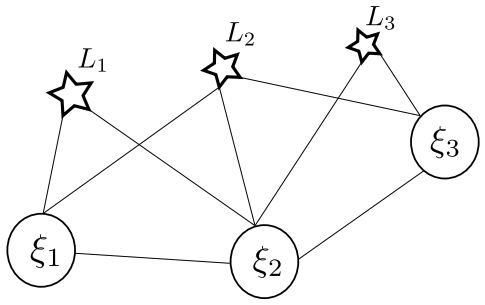
\includegraphics[width=12cm]{bayers_01.png}
\end{figure} 

\begin{enumerate}

\item 绘制系统的信息矩阵 $\Lambda$

\begin{figure}[!h]
  \centering
  
\definecolor{c80b3ff}{RGB}{128,179,255}
\definecolor{cffffff}{RGB}{255,255,255}


\begin{tikzpicture}[y=0.80pt, x=0.80pt, yscale=-1.000000, xscale=1.000000, inner sep=0pt, outer sep=0pt]
  \path[draw=black,fill=c80b3ff,miter limit=4.00,line width=1.500pt,rounded
    corners=0.0000cm] (215.9988,190.6416) rectangle (265.8080,237.5937);
  \path[draw=black,fill=c80b3ff,miter limit=4.00,line width=1.500pt,rounded
    corners=0.0000cm] (265.8080,190.6416) rectangle (315.6172,237.5937);
  \path[draw=black,miter limit=4.00,line width=1.500pt,rounded corners=0.0000cm]
    (315.6172,190.6416) rectangle (365.4264,237.5937);
  \path[draw=black,fill=c80b3ff,miter limit=4.00,line width=1.500pt,rounded
    corners=0.0000cm] (365.4264,190.6416) rectangle (415.2356,237.5937);
  \path[draw=black,fill=c80b3ff,miter limit=4.00,line width=1.500pt,rounded
    corners=0.0000cm] (415.2356,190.6416) rectangle (465.0448,237.5937);
  \path[draw=black,fill=c80b3ff,miter limit=4.00,line width=1.500pt,rounded
    corners=0.0000cm] (215.9988,237.5937) rectangle (265.8080,284.5458);
  \path[draw=black,fill=c80b3ff,miter limit=4.00,line width=1.500pt,rounded
    corners=0.0000cm] (265.8080,237.5937) rectangle (315.6172,284.5458);
  \path[draw=black,fill=c80b3ff,miter limit=4.00,line width=1.500pt,rounded
    corners=0.0000cm] (315.6172,237.5937) rectangle (365.4264,284.5458);
  \path[draw=black,fill=c80b3ff,miter limit=4.00,line width=1.500pt,rounded
    corners=0.0000cm] (365.4264,237.5937) rectangle (415.2356,284.5458);
  \path[draw=black,fill=c80b3ff,miter limit=4.00,line width=1.500pt,rounded
    corners=0.0000cm] (415.2356,237.5937) rectangle (465.0448,284.5458);
  \path[draw=black,miter limit=4.00,line width=1.500pt,rounded corners=0.0000cm]
    (215.9988,284.5458) rectangle (265.8080,331.4979);
  \path[draw=black,fill=c80b3ff,miter limit=4.00,line width=1.500pt,rounded
    corners=0.0000cm] (265.8080,284.5458) rectangle (315.6172,331.4979);
  \path[draw=black,fill=c80b3ff,miter limit=4.00,line width=1.500pt,rounded
    corners=0.0000cm] (315.6172,284.5458) rectangle (365.4264,331.4979);
  \path[draw=black,miter limit=4.00,line width=1.500pt,rounded corners=0.0000cm]
    (365.4264,284.5458) rectangle (415.2356,331.4979);
  \path[draw=black,fill=c80b3ff,miter limit=4.00,line width=1.500pt,rounded
    corners=0.0000cm] (415.2356,284.5458) rectangle (465.0448,331.4979);
  \path[draw=black,fill=c80b3ff,miter limit=4.00,line width=1.500pt,rounded
    corners=0.0000cm] (215.9988,331.4978) rectangle (265.8080,378.4499);
  \path[draw=black,fill=c80b3ff,miter limit=4.00,line width=1.500pt,rounded
    corners=0.0000cm] (265.8080,331.4978) rectangle (315.6172,378.4499);
  \path[draw=black,miter limit=4.00,line width=1.500pt,rounded corners=0.0000cm]
    (315.6172,331.4978) rectangle (365.4264,378.4499);
  \path[draw=black,fill=c80b3ff,miter limit=4.00,line width=1.500pt,rounded
    corners=0.0000cm] (365.4264,331.4978) rectangle (415.2356,378.4499);
  \path[draw=black,fill=cffffff,miter limit=4.00,line width=1.500pt,rounded
    corners=0.0000cm] (415.2356,331.4978) rectangle (465.0448,378.4499);
  \path[draw=black,fill=c80b3ff,miter limit=4.00,line width=1.500pt,rounded
    corners=0.0000cm] (215.9988,378.4500) rectangle (265.8080,425.4020);
  \path[draw=black,fill=c80b3ff,miter limit=4.00,line width=1.500pt,rounded
    corners=0.0000cm] (265.8080,378.4500) rectangle (315.6172,425.4020);
  \path[draw=black,fill=c80b3ff,miter limit=4.00,line width=1.500pt,rounded
    corners=0.0000cm] (315.6172,378.4500) rectangle (365.4264,425.4020);
  \path[draw=black,miter limit=4.00,line width=1.500pt,rounded corners=0.0000cm]
    (365.4264,378.4500) rectangle (415.2356,425.4020);
  \path[draw=black,fill=c80b3ff,miter limit=4.00,line width=1.500pt,rounded
    corners=0.0000cm] (415.2356,378.4500) rectangle (465.0448,425.4020);
  \path[draw=black,miter limit=4.00,line width=1.500pt,rounded corners=0.0000cm]
    (465.0448,190.6416) rectangle (514.8540,237.5937);
  \path[draw=black,fill=c80b3ff,miter limit=4.00,line width=1.500pt,rounded
    corners=0.0000cm] (465.0448,237.5937) rectangle (514.8540,284.5458);
  \path[draw=black,fill=c80b3ff,miter limit=4.00,line width=1.500pt,rounded
    corners=0.0000cm] (465.0448,284.5458) rectangle (514.8540,331.4979);
  \path[draw=black,miter limit=4.00,line width=1.500pt,rounded corners=0.0000cm]
    (465.0448,331.4978) rectangle (514.8540,378.4499);
  \path[draw=black,miter limit=4.00,line width=1.500pt,rounded corners=0.0000cm]
    (465.0448,378.4500) rectangle (514.8540,425.4020);
  \path[draw=black,miter limit=4.00,line width=1.500pt,rounded corners=0.0000cm]
    (215.9988,425.4020) rectangle (265.8080,472.3541);
  \path[draw=black,fill=c80b3ff,miter limit=4.00,line width=1.500pt,rounded
    corners=0.0000cm] (265.8080,425.4020) rectangle (315.6172,472.3541);
  \path[draw=black,fill=c80b3ff,miter limit=4.00,line width=1.500pt,rounded
    corners=0.0000cm] (315.6172,425.4020) rectangle (365.4264,472.3541);
  \path[draw=black,miter limit=4.00,line width=1.500pt,rounded corners=0.0000cm]
    (365.4264,425.4020) rectangle (415.2356,472.3541);
  \path[draw=black,fill=cffffff,miter limit=4.00,line width=1.500pt,rounded
    corners=0.0000cm] (415.2356,425.4020) rectangle (465.0448,472.3541);
  \path[draw=black,fill=c80b3ff,miter limit=4.00,line width=1.500pt,rounded
    corners=0.0000cm] (465.0448,425.4020) rectangle (514.8540,472.3541);
  \begin{scope}[cm={{3.15675,0.0,0.0,-3.15462,(-242.22059,2411.3992)}},draw=black,line join=miter,line cap=butt,miter limit=10.43,even odd rule]
    \path[draw,fill=black,line width=0.000pt] (150.2400,710.1800) --
      (150.1400,710.1100) -- (150.0500,710.0400) -- (149.9600,709.9700) --
      (149.8800,709.9000) -- (149.8000,709.8300) -- (149.7200,709.7500) --
      (149.6500,709.6800) -- (149.5800,709.6100) -- (149.5200,709.5400) --
      (149.4600,709.4600) -- (149.4100,709.3900) -- (149.3600,709.3200) --
      (149.3100,709.2500) -- (149.2700,709.1700) -- (149.2300,709.1000) --
      (149.1900,709.0300) -- (149.1600,708.9600) -- (149.1200,708.9000) --
      (149.1000,708.8300) -- (149.0700,708.7700) -- (149.0500,708.7000) --
      (149.0300,708.6400) -- (149.0100,708.5800) -- (149.0000,708.5300) --
      (148.9800,708.4700) -- (148.9700,708.4200) -- (148.9600,708.3700) --
      (148.9600,708.3200) -- (148.9500,708.2800) -- (148.9500,708.2300) --
      (148.9500,708.2000) -- (148.9500,708.1600) .. controls (148.9500,707.6900) and
      (149.2100,707.4100) .. (149.2300,707.3800) .. controls (149.5400,707.0500) and
      (149.6300,707.0000) .. (150.3800,706.7400) -- (151.5900,706.2700) .. controls
      (151.7300,706.1900) and (151.9300,706.1300) .. (151.9300,705.8300) .. controls
      (151.9300,705.6100) and (151.7600,705.3200) .. (151.4500,705.3200) .. controls
      (151.0100,705.3200) and (150.6800,705.5500) .. (150.5700,705.6300) .. controls
      (150.5100,705.6800) and (150.4900,705.6800) .. (150.4600,705.6800) .. controls
      (150.3800,705.6800) and (150.3700,705.6100) .. (150.3700,705.5700) .. controls
      (150.3700,705.4600) and (150.8800,705.1000) .. (151.4500,705.1000) .. controls
      (152.0500,705.1000) and (152.4800,705.6800) .. (152.4800,706.1600) .. controls
      (152.4800,706.6300) and (152.1000,706.8200) .. (151.9900,706.8600) .. controls
      (151.8700,706.9100) and (151.5200,707.0300) .. (151.4000,707.0800) .. controls
      (151.2000,707.1800) and (150.9900,707.2500) .. (150.7900,707.3200) --
      (150.2000,707.5500) .. controls (149.7400,707.7400) and (149.4500,708.0200) ..
      (149.4500,708.4400) .. controls (149.4500,708.8500) and (149.8400,709.7100) ..
      (150.6600,710.1300) .. controls (151.0400,710.0000) and (151.3400,710.0000) ..
      (151.5400,710.0000) .. controls (151.8400,710.0000) and (152.4600,710.0000) ..
      (152.4600,710.3000) .. controls (152.4600,710.5500) and (152.0400,710.5800) ..
      (151.6500,710.5800) -- (151.6500,710.3600) .. controls (151.9900,710.3600) and
      (152.0200,710.3500) .. (152.2100,710.3000) .. controls (152.1300,710.2500) and
      (152.0200,710.2200) .. (151.5700,710.2200) .. controls (151.3400,710.2200) and
      (151.2600,710.2200) .. (151.0700,710.3000) -- (151.0700,710.3000) .. controls
      (151.3000,710.3600) and (151.5200,710.3600) .. (151.6500,710.3600) --
      (151.6500,710.5800) .. controls (151.4800,710.5800) and (151.1800,710.5800) ..
      (150.8000,710.4600) .. controls (150.5500,710.7200) and (150.5200,711.0300) ..
      (150.5200,711.2400) .. controls (150.5200,711.7800) and (150.8800,712.5500) ..
      (151.6200,712.9300) .. controls (151.8000,712.7100) and (152.0200,712.7100) ..
      (152.2600,712.7100) .. controls (152.5100,712.7100) and (153.1500,712.7100) ..
      (153.1500,713.0000) .. controls (153.1500,713.2700) and (152.7100,713.2800) ..
      (152.3200,713.2800) -- (152.3200,713.0700) .. controls (152.6600,713.0700) and
      (152.7100,713.0500) .. (152.8800,713.0000) .. controls (152.8000,712.9700) and
      (152.7100,712.9300) .. (152.2700,712.9300) .. controls (152.0900,712.9300) and
      (151.9600,712.9300) .. (151.8500,713.0000) -- (151.8500,713.0000) .. controls
      (152.0100,713.0700) and (152.2100,713.0700) .. (152.3200,713.0700) --
      (152.3200,713.2800) .. controls (152.2000,713.2800) and (151.9500,713.2800) ..
      (151.6800,713.2200) .. controls (151.6600,713.3200) and (151.6500,713.4000) ..
      (151.6500,713.5500) .. controls (151.6500,713.6900) and (151.7000,713.9100) ..
      (151.7000,713.9300) .. controls (151.7000,714.0000) and (151.6500,714.0500) ..
      (151.5700,714.0500) .. controls (151.4000,714.0500) and (151.4000,713.6000) ..
      (151.4000,713.5700) .. controls (151.4000,713.3600) and (151.4500,713.2200) ..
      (151.4500,713.1800) .. controls (150.4000,712.8800) and (149.7300,712.0800) ..
      (149.7300,711.3200) .. controls (149.7300,710.9600) and (149.9000,710.5300) ..
      (150.3700,710.2700) -- cycle;
    \path[draw,fill=black,line width=0.000pt] (155.4300,710.1000) --
      (155.4300,710.1100) -- (155.4300,710.1200) -- (155.4300,710.1200) --
      (155.4300,710.1300) -- (155.4300,710.1400) -- (155.4300,710.1500) --
      (155.4300,710.1500) -- (155.4300,710.1600) -- (155.4300,710.1700) --
      (155.4300,710.1700) -- (155.4300,710.1900) -- (155.4300,710.2000) --
      (155.4200,710.2100) -- (155.4200,710.2200) -- (155.4200,710.2300) --
      (155.4200,710.2400) -- (155.4100,710.2400) -- (155.4100,710.2500) --
      (155.4100,710.2600) -- (155.4000,710.2600) -- (155.4000,710.2700) --
      (155.3900,710.2700) -- (155.3800,710.2800) -- (155.3800,710.2800) --
      (155.3700,710.2900) -- (155.3600,710.2900) -- (155.3500,710.2900) --
      (155.3400,710.2900) -- (155.3400,710.2900) -- (155.3300,710.3000) --
      (155.3300,710.3000) -- (155.3200,710.3000) -- (155.3100,710.3000) --
      (155.3100,710.3000) -- (155.3000,710.3000) -- (155.2900,710.3000) --
      (155.2900,710.3000) -- (155.2800,710.3000) -- (155.2700,710.3000) --
      (155.2600,710.3000) -- (155.2600,710.3000) -- (155.2500,710.3000) --
      (155.2400,710.3000) -- (155.2300,710.3000) -- (155.2200,710.3000) --
      (155.2100,710.3000) .. controls (154.7600,709.8500) and (154.1200,709.8500) ..
      (153.8400,709.8500) -- (153.8400,709.6000) .. controls (154.0100,709.6000) and
      (154.4800,709.6000) .. (154.8500,709.7800) -- (154.8500,706.2100) .. controls
      (154.8500,705.9700) and (154.8500,705.8800) .. (154.1500,705.8800) --
      (153.8800,705.8800) -- (153.8800,705.6300) .. controls (154.0100,705.6300) and
      (154.8800,705.6600) .. (155.1300,705.6600) .. controls (155.3500,705.6600) and
      (156.2400,705.6300) .. (156.4000,705.6300) -- (156.4000,705.8800) --
      (156.1300,705.8800) .. controls (155.4300,705.8800) and (155.4300,705.9700) ..
      (155.4300,706.2100) -- cycle;
  \end{scope}
  \begin{scope}[cm={{3.15675,0.0,0.0,-3.15462,(-193.56943,2411.3985)}},draw=black,line join=miter,line cap=butt,miter limit=10.43,even odd rule]
    \path[draw=black,fill=black,line width=0.000pt] (150.2400,710.1800) --
      (150.1400,710.1100) -- (150.0500,710.0400) -- (149.9600,709.9700) --
      (149.8800,709.9000) -- (149.8000,709.8300) -- (149.7200,709.7500) --
      (149.6500,709.6800) -- (149.5800,709.6100) -- (149.5200,709.5400) --
      (149.4600,709.4600) -- (149.4100,709.3900) -- (149.3600,709.3200) --
      (149.3100,709.2500) -- (149.2700,709.1700) -- (149.2300,709.1000) --
      (149.1900,709.0300) -- (149.1600,708.9600) -- (149.1200,708.9000) --
      (149.1000,708.8300) -- (149.0700,708.7700) -- (149.0500,708.7000) --
      (149.0300,708.6400) -- (149.0100,708.5800) -- (149.0000,708.5300) --
      (148.9800,708.4700) -- (148.9700,708.4200) -- (148.9600,708.3700) --
      (148.9600,708.3200) -- (148.9500,708.2800) -- (148.9500,708.2300) --
      (148.9500,708.2000) -- (148.9500,708.1600) .. controls (148.9500,707.6900) and
      (149.2100,707.4100) .. (149.2300,707.3800) .. controls (149.5400,707.0500) and
      (149.6300,707.0000) .. (150.3800,706.7400) -- (151.5900,706.2700) .. controls
      (151.7300,706.1900) and (151.9300,706.1300) .. (151.9300,705.8300) .. controls
      (151.9300,705.6100) and (151.7600,705.3200) .. (151.4500,705.3200) .. controls
      (151.0100,705.3200) and (150.6800,705.5500) .. (150.5700,705.6300) .. controls
      (150.5100,705.6800) and (150.4900,705.6800) .. (150.4600,705.6800) .. controls
      (150.3800,705.6800) and (150.3700,705.6100) .. (150.3700,705.5700) .. controls
      (150.3700,705.4600) and (150.8800,705.1000) .. (151.4500,705.1000) .. controls
      (152.0500,705.1000) and (152.4800,705.6800) .. (152.4800,706.1600) .. controls
      (152.4800,706.6300) and (152.1000,706.8200) .. (151.9900,706.8600) .. controls
      (151.8700,706.9100) and (151.5200,707.0300) .. (151.4000,707.0800) .. controls
      (151.2000,707.1800) and (150.9900,707.2500) .. (150.7900,707.3200) --
      (150.2000,707.5500) .. controls (149.7400,707.7400) and (149.4500,708.0200) ..
      (149.4500,708.4400) .. controls (149.4500,708.8500) and (149.8400,709.7100) ..
      (150.6600,710.1300) .. controls (151.0400,710.0000) and (151.3400,710.0000) ..
      (151.5400,710.0000) .. controls (151.8400,710.0000) and (152.4600,710.0000) ..
      (152.4600,710.3000) .. controls (152.4600,710.5500) and (152.0400,710.5800) ..
      (151.6500,710.5800) -- (151.6500,710.3600) .. controls (151.9900,710.3600) and
      (152.0200,710.3500) .. (152.2100,710.3000) .. controls (152.1300,710.2500) and
      (152.0200,710.2200) .. (151.5700,710.2200) .. controls (151.3400,710.2200) and
      (151.2600,710.2200) .. (151.0700,710.3000) -- (151.0700,710.3000) .. controls
      (151.3000,710.3600) and (151.5200,710.3600) .. (151.6500,710.3600) --
      (151.6500,710.5800) .. controls (151.4800,710.5800) and (151.1800,710.5800) ..
      (150.8000,710.4600) .. controls (150.5500,710.7200) and (150.5200,711.0300) ..
      (150.5200,711.2400) .. controls (150.5200,711.7800) and (150.8800,712.5500) ..
      (151.6200,712.9300) .. controls (151.8000,712.7100) and (152.0200,712.7100) ..
      (152.2600,712.7100) .. controls (152.5100,712.7100) and (153.1500,712.7100) ..
      (153.1500,713.0000) .. controls (153.1500,713.2700) and (152.7100,713.2800) ..
      (152.3200,713.2800) -- (152.3200,713.0700) .. controls (152.6600,713.0700) and
      (152.7100,713.0500) .. (152.8800,713.0000) .. controls (152.8000,712.9700) and
      (152.7100,712.9300) .. (152.2700,712.9300) .. controls (152.0900,712.9300) and
      (151.9600,712.9300) .. (151.8500,713.0000) -- (151.8500,713.0000) .. controls
      (152.0100,713.0700) and (152.2100,713.0700) .. (152.3200,713.0700) --
      (152.3200,713.2800) .. controls (152.2000,713.2800) and (151.9500,713.2800) ..
      (151.6800,713.2200) .. controls (151.6600,713.3200) and (151.6500,713.4000) ..
      (151.6500,713.5500) .. controls (151.6500,713.6900) and (151.7000,713.9100) ..
      (151.7000,713.9300) .. controls (151.7000,714.0000) and (151.6500,714.0500) ..
      (151.5700,714.0500) .. controls (151.4000,714.0500) and (151.4000,713.6000) ..
      (151.4000,713.5700) .. controls (151.4000,713.3600) and (151.4500,713.2200) ..
      (151.4500,713.1800) .. controls (150.4000,712.8800) and (149.7300,712.0800) ..
      (149.7300,711.3200) .. controls (149.7300,710.9600) and (149.9000,710.5300) ..
      (150.3700,710.2700) -- cycle;
    \path[draw=black,fill=black,line width=0.000pt] (156.6200,706.9100) --
      (156.3800,706.9100) .. controls (156.3700,706.7500) and (156.2900,706.3300) ..
      (156.2000,706.2700) .. controls (156.1500,706.2200) and (155.6000,706.2200) ..
      (155.5100,706.2200) -- (154.2100,706.2200) .. controls (154.9500,706.8800) and
      (155.2000,707.0800) .. (155.6200,707.4100) .. controls (156.1300,707.8200) and
      (156.6200,708.2500) .. (156.6200,708.9300) .. controls (156.6200,709.7700) and
      (155.8800,710.3000) .. (154.9800,710.3000) .. controls (154.1000,710.3000) and
      (153.5100,709.6900) .. (153.5100,709.0300) .. controls (153.5100,708.6800) and
      (153.8200,708.6500) .. (153.8800,708.6500) .. controls (154.0500,708.6500) and
      (154.2600,708.7700) .. (154.2600,709.0200) .. controls (154.2600,709.1500) and
      (154.2100,709.4000) .. (153.8400,709.4000) .. controls (154.0500,709.9000) and
      (154.5400,710.0500) .. (154.8700,710.0500) .. controls (155.5700,710.0500) and
      (155.9500,709.4900) .. (155.9500,708.9300) .. controls (155.9500,708.3200) and
      (155.5100,707.8300) .. (155.2700,707.5800) -- (153.5900,705.9100) .. controls
      (153.5100,705.8300) and (153.5100,705.8300) .. (153.5100,705.6300) --
      (156.4100,705.6300) -- cycle;
  \end{scope}
  \begin{scope}[cm={{3.15675,0.0,0.0,-3.15462,(-144.13673,2411.3985)}},draw=black,line join=miter,line cap=butt,miter limit=10.43,even odd rule]
    \path[draw=black,fill=black,line width=0.000pt] (150.2400,710.1800) --
      (150.1400,710.1100) -- (150.0500,710.0400) -- (149.9600,709.9700) --
      (149.8800,709.9000) -- (149.8000,709.8300) -- (149.7200,709.7500) --
      (149.6500,709.6800) -- (149.5800,709.6100) -- (149.5200,709.5400) --
      (149.4600,709.4600) -- (149.4100,709.3900) -- (149.3600,709.3200) --
      (149.3100,709.2500) -- (149.2700,709.1700) -- (149.2300,709.1000) --
      (149.1900,709.0300) -- (149.1600,708.9600) -- (149.1200,708.9000) --
      (149.1000,708.8300) -- (149.0700,708.7700) -- (149.0500,708.7000) --
      (149.0300,708.6400) -- (149.0100,708.5800) -- (149.0000,708.5300) --
      (148.9800,708.4700) -- (148.9700,708.4200) -- (148.9600,708.3700) --
      (148.9600,708.3200) -- (148.9500,708.2800) -- (148.9500,708.2300) --
      (148.9500,708.2000) -- (148.9500,708.1600) .. controls (148.9500,707.6900) and
      (149.2100,707.4100) .. (149.2300,707.3800) .. controls (149.5400,707.0500) and
      (149.6300,707.0000) .. (150.3800,706.7400) -- (151.5900,706.2700) .. controls
      (151.7300,706.1900) and (151.9300,706.1300) .. (151.9300,705.8300) .. controls
      (151.9300,705.6100) and (151.7600,705.3200) .. (151.4500,705.3200) .. controls
      (151.0100,705.3200) and (150.6800,705.5500) .. (150.5700,705.6300) .. controls
      (150.5100,705.6800) and (150.4900,705.6800) .. (150.4600,705.6800) .. controls
      (150.3800,705.6800) and (150.3700,705.6100) .. (150.3700,705.5700) .. controls
      (150.3700,705.4600) and (150.8800,705.1000) .. (151.4500,705.1000) .. controls
      (152.0500,705.1000) and (152.4800,705.6800) .. (152.4800,706.1600) .. controls
      (152.4800,706.6300) and (152.1000,706.8200) .. (151.9900,706.8600) .. controls
      (151.8700,706.9100) and (151.5200,707.0300) .. (151.4000,707.0800) .. controls
      (151.2000,707.1800) and (150.9900,707.2500) .. (150.7900,707.3200) --
      (150.2000,707.5500) .. controls (149.7400,707.7400) and (149.4500,708.0200) ..
      (149.4500,708.4400) .. controls (149.4500,708.8500) and (149.8400,709.7100) ..
      (150.6600,710.1300) .. controls (151.0400,710.0000) and (151.3400,710.0000) ..
      (151.5400,710.0000) .. controls (151.8400,710.0000) and (152.4600,710.0000) ..
      (152.4600,710.3000) .. controls (152.4600,710.5500) and (152.0400,710.5800) ..
      (151.6500,710.5800) -- (151.6500,710.3600) .. controls (151.9900,710.3600) and
      (152.0200,710.3500) .. (152.2100,710.3000) .. controls (152.1300,710.2500) and
      (152.0200,710.2200) .. (151.5700,710.2200) .. controls (151.3400,710.2200) and
      (151.2600,710.2200) .. (151.0700,710.3000) -- (151.0700,710.3000) .. controls
      (151.3000,710.3600) and (151.5200,710.3600) .. (151.6500,710.3600) --
      (151.6500,710.5800) .. controls (151.4800,710.5800) and (151.1800,710.5800) ..
      (150.8000,710.4600) .. controls (150.5500,710.7200) and (150.5200,711.0300) ..
      (150.5200,711.2400) .. controls (150.5200,711.7800) and (150.8800,712.5500) ..
      (151.6200,712.9300) .. controls (151.8000,712.7100) and (152.0200,712.7100) ..
      (152.2600,712.7100) .. controls (152.5100,712.7100) and (153.1500,712.7100) ..
      (153.1500,713.0000) .. controls (153.1500,713.2700) and (152.7100,713.2800) ..
      (152.3200,713.2800) -- (152.3200,713.0700) .. controls (152.6600,713.0700) and
      (152.7100,713.0500) .. (152.8800,713.0000) .. controls (152.8000,712.9700) and
      (152.7100,712.9300) .. (152.2700,712.9300) .. controls (152.0900,712.9300) and
      (151.9600,712.9300) .. (151.8500,713.0000) -- (151.8500,713.0000) .. controls
      (152.0100,713.0700) and (152.2100,713.0700) .. (152.3200,713.0700) --
      (152.3200,713.2800) .. controls (152.2000,713.2800) and (151.9500,713.2800) ..
      (151.6800,713.2200) .. controls (151.6600,713.3200) and (151.6500,713.4000) ..
      (151.6500,713.5500) .. controls (151.6500,713.6900) and (151.7000,713.9100) ..
      (151.7000,713.9300) .. controls (151.7000,714.0000) and (151.6500,714.0500) ..
      (151.5700,714.0500) .. controls (151.4000,714.0500) and (151.4000,713.6000) ..
      (151.4000,713.5700) .. controls (151.4000,713.3600) and (151.4500,713.2200) ..
      (151.4500,713.1800) .. controls (150.4000,712.8800) and (149.7300,712.0800) ..
      (149.7300,711.3200) .. controls (149.7300,710.9600) and (149.9000,710.5300) ..
      (150.3700,710.2700) -- cycle;
    \path[draw=black,fill=black,line width=0.000pt] (154.9900,707.9700) --
      (155.0400,707.9700) -- (155.0900,707.9700) -- (155.1400,707.9600) --
      (155.1900,707.9600) -- (155.2400,707.9500) -- (155.2800,707.9300) --
      (155.3300,707.9200) -- (155.3700,707.9000) -- (155.4100,707.8800) --
      (155.4500,707.8600) -- (155.4900,707.8400) -- (155.5300,707.8100) --
      (155.5700,707.7900) -- (155.6000,707.7600) -- (155.6300,707.7300) --
      (155.6700,707.6900) -- (155.7000,707.6600) -- (155.7300,707.6200) --
      (155.7500,707.5800) -- (155.7800,707.5300) -- (155.8000,707.4900) --
      (155.8200,707.4400) -- (155.8400,707.3900) -- (155.8600,707.3400) --
      (155.8800,707.2900) -- (155.8900,707.2300) -- (155.9000,707.1700) --
      (155.9100,707.1100) -- (155.9200,707.0500) -- (155.9300,706.9800) --
      (155.9300,706.9200) -- (155.9300,706.8500) .. controls (155.9300,705.9700) and
      (155.4300,705.7100) .. (155.0200,705.7100) .. controls (154.7400,705.7100) and
      (154.1200,705.7800) .. (153.8200,706.2100) .. controls (154.1500,706.2200) and
      (154.2300,706.4600) .. (154.2300,706.6000) .. controls (154.2300,706.8200) and
      (154.0500,706.9900) .. (153.8400,706.9900) .. controls (153.6500,706.9900) and
      (153.4500,706.8600) .. (153.4500,706.5800) .. controls (153.4500,705.9100) and
      (154.1800,705.4900) .. (155.0400,705.4900) .. controls (156.0100,705.4900) and
      (156.6800,706.1500) .. (156.6800,706.8500) .. controls (156.6800,707.4000) and
      (156.2300,707.9400) .. (155.4600,708.1000) .. controls (156.2000,708.3600) and
      (156.4600,708.9000) .. (156.4600,709.3300) .. controls (156.4600,709.8800) and
      (155.8200,710.3000) .. (155.0400,710.3000) .. controls (154.2600,710.3000) and
      (153.6600,709.9100) .. (153.6600,709.3500) .. controls (153.6600,709.1100) and
      (153.8200,708.9900) .. (154.0400,708.9900) .. controls (154.2600,708.9900) and
      (154.4000,709.1500) .. (154.4000,709.3500) .. controls (154.4000,709.5500) and
      (154.2600,709.6900) .. (154.0400,709.7100) .. controls (154.2700,710.0200) and
      (154.7600,710.1000) .. (155.0200,710.1000) .. controls (155.3400,710.1000) and
      (155.7900,709.9400) .. (155.7900,709.3300) .. controls (155.7900,709.0300) and
      (155.6800,708.7100) .. (155.5100,708.4900) .. controls (155.2700,708.2200) and
      (155.0700,708.2100) .. (154.7300,708.1900) .. controls (154.5400,708.1800) and
      (154.5400,708.1800) .. (154.4900,708.1600) .. controls (154.4800,708.1600) and
      (154.4300,708.1600) .. (154.4300,708.0800) .. controls (154.4300,707.9700) and
      (154.4900,707.9700) .. (154.6200,707.9700) -- cycle;
  \end{scope}
  \begin{scope}[cm={{3.15675,0.0,0.0,-3.15462,(-96.40147,2413.0704)}},draw=black,line join=miter,line cap=butt,miter limit=10.43,even odd rule]
    \path[draw=black,fill=black,line width=0.000pt] (152.4300,713.1500) --
      (152.4400,713.1800) -- (152.4400,713.2100) -- (152.4500,713.2400) --
      (152.4600,713.2700) -- (152.4700,713.3000) -- (152.4800,713.3200) --
      (152.4800,713.3500) -- (152.4900,713.3700) -- (152.5100,713.3900) --
      (152.5200,713.4100) -- (152.5300,713.4300) -- (152.5500,713.4500) --
      (152.5700,713.4700) -- (152.5900,713.4800) -- (152.6100,713.5000) --
      (152.6300,713.5100) -- (152.6600,713.5300) -- (152.6900,713.5400) --
      (152.7200,713.5500) -- (152.7500,713.5600) -- (152.7700,713.5600) --
      (152.7900,713.5700) -- (152.8100,713.5700) -- (152.8300,713.5800) --
      (152.8600,713.5800) -- (152.8800,713.5800) -- (152.9000,713.5900) --
      (152.9300,713.5900) -- (152.9500,713.5900) -- (152.9800,713.6000) --
      (153.0100,713.6000) -- (153.0400,713.6000) -- (153.0700,713.6000) --
      (153.1000,713.6000) -- (153.1300,713.6100) -- (153.1700,713.6100) --
      (153.2000,713.6100) -- (153.2400,713.6100) -- (153.2700,713.6100) --
      (153.3100,713.6100) -- (153.3500,713.6100) -- (153.3900,713.6100) --
      (153.4300,713.6100) -- (153.4800,713.6100) .. controls (153.7700,713.6100) and
      (153.8500,713.6100) .. (153.8500,713.8000) .. controls (153.8500,713.9100) and
      (153.7400,713.9100) .. (153.7000,713.9100) .. controls (153.3700,713.9100) and
      (152.5500,713.8800) .. (152.2300,713.8800) .. controls (151.9300,713.8800) and
      (151.2100,713.9100) .. (150.9100,713.9100) .. controls (150.8400,713.9100) and
      (150.7100,713.9100) .. (150.7100,713.7200) .. controls (150.7100,713.6100) and
      (150.8000,713.6100) .. (150.9900,713.6100) .. controls (151.0100,713.6100) and
      (151.2100,713.6100) .. (151.3700,713.5800) .. controls (151.5500,713.5700) and
      (151.6500,713.5500) .. (151.6500,713.4300) .. controls (151.6500,713.4000) and
      (151.6300,713.3600) .. (151.6000,713.2400) -- (150.2700,707.9100) .. controls
      (150.1600,707.5200) and (150.1500,707.4400) .. (149.3700,707.4400) .. controls
      (149.2000,707.4400) and (149.1000,707.4400) .. (149.1000,707.2400) .. controls
      (149.1000,707.1300) and (149.2000,707.1300) .. (149.3700,707.1300) --
      (153.9600,707.1300) .. controls (154.2100,707.1300) and (154.2100,707.1300) ..
      (154.2700,707.3000) -- (155.0500,709.4400) .. controls (155.1000,709.5500) and
      (155.1000,709.5700) .. (155.1000,709.5800) .. controls (155.1000,709.6300) and
      (155.0700,709.6900) .. (154.9800,709.6900) .. controls (154.8800,709.6900) and
      (154.8800,709.6500) .. (154.8000,709.4900) .. controls (154.4800,708.5700) and
      (154.0400,707.4400) .. (152.3200,707.4400) -- (151.3800,707.4400) .. controls
      (151.2400,707.4400) and (151.2300,707.4400) .. (151.1600,707.4400) .. controls
      (151.0700,707.4600) and (151.0400,707.4700) .. (151.0400,707.5500) .. controls
      (151.0400,707.5800) and (151.0400,707.6000) .. (151.0900,707.7700) -- cycle;
    \path[draw=black,fill=black,line width=0.000pt] (157.8500,710.1000) --
      (157.8500,710.1100) -- (157.8500,710.1200) -- (157.8500,710.1200) --
      (157.8500,710.1300) -- (157.8500,710.1400) -- (157.8500,710.1500) --
      (157.8500,710.1500) -- (157.8500,710.1600) -- (157.8500,710.1700) --
      (157.8500,710.1700) -- (157.8500,710.1900) -- (157.8400,710.2000) --
      (157.8400,710.2100) -- (157.8400,710.2200) -- (157.8400,710.2300) --
      (157.8400,710.2400) -- (157.8300,710.2400) -- (157.8300,710.2500) --
      (157.8200,710.2600) -- (157.8200,710.2600) -- (157.8100,710.2700) --
      (157.8100,710.2700) -- (157.8000,710.2800) -- (157.8000,710.2800) --
      (157.7900,710.2900) -- (157.7800,710.2900) -- (157.7700,710.2900) --
      (157.7600,710.2900) -- (157.7500,710.2900) -- (157.7500,710.3000) --
      (157.7400,710.3000) -- (157.7400,710.3000) -- (157.7300,710.3000) --
      (157.7200,710.3000) -- (157.7200,710.3000) -- (157.7100,710.3000) --
      (157.7000,710.3000) -- (157.7000,710.3000) -- (157.6900,710.3000) --
      (157.6800,710.3000) -- (157.6700,710.3000) -- (157.6600,710.3000) --
      (157.6600,710.3000) -- (157.6500,710.3000) -- (157.6400,710.3000) --
      (157.6300,710.3000) .. controls (157.1800,709.8500) and (156.5400,709.8500) ..
      (156.2500,709.8500) -- (156.2500,709.6000) .. controls (156.4300,709.6000) and
      (156.9000,709.6000) .. (157.2700,709.7800) -- (157.2700,706.2100) .. controls
      (157.2700,705.9700) and (157.2700,705.8800) .. (156.5700,705.8800) --
      (156.3000,705.8800) -- (156.3000,705.6300) .. controls (156.4300,705.6300) and
      (157.3000,705.6600) .. (157.5500,705.6600) .. controls (157.7700,705.6600) and
      (158.6600,705.6300) .. (158.8200,705.6300) -- (158.8200,705.8800) --
      (158.5500,705.8800) .. controls (157.8500,705.8800) and (157.8500,705.9700) ..
      (157.8500,706.2100) -- cycle;
  \end{scope}
  \begin{scope}[cm={{3.15675,0.0,0.0,-3.15462,(-48.0052,2413.0704)}},draw=black,line join=miter,line cap=butt,miter limit=10.43,even odd rule]
    \path[draw=black,fill=black,line width=0.000pt] (152.4300,713.1500) --
      (152.4400,713.1800) -- (152.4400,713.2100) -- (152.4500,713.2400) --
      (152.4600,713.2700) -- (152.4700,713.3000) -- (152.4800,713.3200) --
      (152.4800,713.3500) -- (152.4900,713.3700) -- (152.5100,713.3900) --
      (152.5200,713.4100) -- (152.5300,713.4300) -- (152.5500,713.4500) --
      (152.5700,713.4700) -- (152.5900,713.4800) -- (152.6100,713.5000) --
      (152.6300,713.5100) -- (152.6600,713.5300) -- (152.6900,713.5400) --
      (152.7200,713.5500) -- (152.7500,713.5600) -- (152.7700,713.5600) --
      (152.7900,713.5700) -- (152.8100,713.5700) -- (152.8300,713.5800) --
      (152.8600,713.5800) -- (152.8800,713.5800) -- (152.9000,713.5900) --
      (152.9300,713.5900) -- (152.9500,713.5900) -- (152.9800,713.6000) --
      (153.0100,713.6000) -- (153.0400,713.6000) -- (153.0700,713.6000) --
      (153.1000,713.6000) -- (153.1300,713.6100) -- (153.1700,713.6100) --
      (153.2000,713.6100) -- (153.2400,713.6100) -- (153.2700,713.6100) --
      (153.3100,713.6100) -- (153.3500,713.6100) -- (153.3900,713.6100) --
      (153.4300,713.6100) -- (153.4800,713.6100) .. controls (153.7700,713.6100) and
      (153.8500,713.6100) .. (153.8500,713.8000) .. controls (153.8500,713.9100) and
      (153.7400,713.9100) .. (153.7000,713.9100) .. controls (153.3700,713.9100) and
      (152.5500,713.8800) .. (152.2300,713.8800) .. controls (151.9300,713.8800) and
      (151.2100,713.9100) .. (150.9100,713.9100) .. controls (150.8400,713.9100) and
      (150.7100,713.9100) .. (150.7100,713.7200) .. controls (150.7100,713.6100) and
      (150.8000,713.6100) .. (150.9900,713.6100) .. controls (151.0100,713.6100) and
      (151.2100,713.6100) .. (151.3700,713.5800) .. controls (151.5500,713.5700) and
      (151.6500,713.5500) .. (151.6500,713.4300) .. controls (151.6500,713.4000) and
      (151.6300,713.3600) .. (151.6000,713.2400) -- (150.2700,707.9100) .. controls
      (150.1600,707.5200) and (150.1500,707.4400) .. (149.3700,707.4400) .. controls
      (149.2000,707.4400) and (149.1000,707.4400) .. (149.1000,707.2400) .. controls
      (149.1000,707.1300) and (149.2000,707.1300) .. (149.3700,707.1300) --
      (153.9600,707.1300) .. controls (154.2100,707.1300) and (154.2100,707.1300) ..
      (154.2700,707.3000) -- (155.0500,709.4400) .. controls (155.1000,709.5500) and
      (155.1000,709.5700) .. (155.1000,709.5800) .. controls (155.1000,709.6300) and
      (155.0700,709.6900) .. (154.9800,709.6900) .. controls (154.8800,709.6900) and
      (154.8800,709.6500) .. (154.8000,709.4900) .. controls (154.4800,708.5700) and
      (154.0400,707.4400) .. (152.3200,707.4400) -- (151.3800,707.4400) .. controls
      (151.2400,707.4400) and (151.2300,707.4400) .. (151.1600,707.4400) .. controls
      (151.0700,707.4600) and (151.0400,707.4700) .. (151.0400,707.5500) .. controls
      (151.0400,707.5800) and (151.0400,707.6000) .. (151.0900,707.7700) -- cycle;
    \path[draw=black,fill=black,line width=0.000pt] (159.0400,706.9100) --
      (158.8000,706.9100) .. controls (158.7900,706.7500) and (158.7100,706.3300) ..
      (158.6100,706.2700) .. controls (158.5700,706.2200) and (158.0200,706.2200) ..
      (157.9300,706.2200) -- (156.6300,706.2200) .. controls (157.3600,706.8800) and
      (157.6100,707.0800) .. (158.0400,707.4100) .. controls (158.5500,707.8200) and
      (159.0400,708.2500) .. (159.0400,708.9300) .. controls (159.0400,709.7700) and
      (158.3000,710.3000) .. (157.4000,710.3000) .. controls (156.5200,710.3000) and
      (155.9300,709.6900) .. (155.9300,709.0300) .. controls (155.9300,708.6800) and
      (156.2400,708.6500) .. (156.3000,708.6500) .. controls (156.4700,708.6500) and
      (156.6800,708.7700) .. (156.6800,709.0200) .. controls (156.6800,709.1500) and
      (156.6300,709.4000) .. (156.2500,709.4000) .. controls (156.4700,709.9000) and
      (156.9600,710.0500) .. (157.2900,710.0500) .. controls (157.9900,710.0500) and
      (158.3600,709.4900) .. (158.3600,708.9300) .. controls (158.3600,708.3200) and
      (157.9300,707.8300) .. (157.6900,707.5800) -- (156.0000,705.9100) .. controls
      (155.9300,705.8300) and (155.9300,705.8300) .. (155.9300,705.6300) --
      (158.8300,705.6300) -- cycle;
  \end{scope}
  \begin{scope}[cm={{3.15675,0.0,0.0,-3.15462,(2.23995,2412.6288)}},draw=black,line join=miter,line cap=butt,miter limit=10.43,even odd rule]
    \path[draw=black,fill=black,line width=0.000pt] (152.4300,713.1500) --
      (152.4400,713.1800) -- (152.4400,713.2100) -- (152.4500,713.2400) --
      (152.4600,713.2700) -- (152.4700,713.3000) -- (152.4800,713.3200) --
      (152.4800,713.3500) -- (152.4900,713.3700) -- (152.5100,713.3900) --
      (152.5200,713.4100) -- (152.5300,713.4300) -- (152.5500,713.4500) --
      (152.5700,713.4700) -- (152.5900,713.4800) -- (152.6100,713.5000) --
      (152.6300,713.5100) -- (152.6600,713.5300) -- (152.6900,713.5400) --
      (152.7200,713.5500) -- (152.7500,713.5600) -- (152.7700,713.5600) --
      (152.7900,713.5700) -- (152.8100,713.5700) -- (152.8300,713.5800) --
      (152.8600,713.5800) -- (152.8800,713.5800) -- (152.9000,713.5900) --
      (152.9300,713.5900) -- (152.9500,713.5900) -- (152.9800,713.6000) --
      (153.0100,713.6000) -- (153.0400,713.6000) -- (153.0700,713.6000) --
      (153.1000,713.6000) -- (153.1300,713.6100) -- (153.1700,713.6100) --
      (153.2000,713.6100) -- (153.2400,713.6100) -- (153.2700,713.6100) --
      (153.3100,713.6100) -- (153.3500,713.6100) -- (153.3900,713.6100) --
      (153.4300,713.6100) -- (153.4800,713.6100) .. controls (153.7700,713.6100) and
      (153.8500,713.6100) .. (153.8500,713.8000) .. controls (153.8500,713.9100) and
      (153.7400,713.9100) .. (153.7000,713.9100) .. controls (153.3700,713.9100) and
      (152.5500,713.8800) .. (152.2300,713.8800) .. controls (151.9300,713.8800) and
      (151.2100,713.9100) .. (150.9100,713.9100) .. controls (150.8400,713.9100) and
      (150.7100,713.9100) .. (150.7100,713.7200) .. controls (150.7100,713.6100) and
      (150.8000,713.6100) .. (150.9900,713.6100) .. controls (151.0100,713.6100) and
      (151.2100,713.6100) .. (151.3700,713.5800) .. controls (151.5500,713.5700) and
      (151.6500,713.5500) .. (151.6500,713.4300) .. controls (151.6500,713.4000) and
      (151.6300,713.3600) .. (151.6000,713.2400) -- (150.2700,707.9100) .. controls
      (150.1600,707.5200) and (150.1500,707.4400) .. (149.3700,707.4400) .. controls
      (149.2000,707.4400) and (149.1000,707.4400) .. (149.1000,707.2400) .. controls
      (149.1000,707.1300) and (149.2000,707.1300) .. (149.3700,707.1300) --
      (153.9600,707.1300) .. controls (154.2100,707.1300) and (154.2100,707.1300) ..
      (154.2700,707.3000) -- (155.0500,709.4400) .. controls (155.1000,709.5500) and
      (155.1000,709.5700) .. (155.1000,709.5800) .. controls (155.1000,709.6300) and
      (155.0700,709.6900) .. (154.9800,709.6900) .. controls (154.8800,709.6900) and
      (154.8800,709.6500) .. (154.8000,709.4900) .. controls (154.4800,708.5700) and
      (154.0400,707.4400) .. (152.3200,707.4400) -- (151.3800,707.4400) .. controls
      (151.2400,707.4400) and (151.2300,707.4400) .. (151.1600,707.4400) .. controls
      (151.0700,707.4600) and (151.0400,707.4700) .. (151.0400,707.5500) .. controls
      (151.0400,707.5800) and (151.0400,707.6000) .. (151.0900,707.7700) -- cycle;
    \path[draw=black,fill=black,line width=0.000pt] (157.4100,707.9700) --
      (157.4600,707.9700) -- (157.5100,707.9700) -- (157.5600,707.9600) --
      (157.6100,707.9600) -- (157.6500,707.9500) -- (157.7000,707.9300) --
      (157.7400,707.9200) -- (157.7900,707.9000) -- (157.8300,707.8800) --
      (157.8700,707.8600) -- (157.9100,707.8400) -- (157.9500,707.8100) --
      (157.9800,707.7900) -- (158.0200,707.7600) -- (158.0500,707.7300) --
      (158.0800,707.6900) -- (158.1100,707.6600) -- (158.1400,707.6200) --
      (158.1700,707.5800) -- (158.2000,707.5300) -- (158.2200,707.4900) --
      (158.2400,707.4400) -- (158.2600,707.3900) -- (158.2800,707.3400) --
      (158.2900,707.2900) -- (158.3100,707.2300) -- (158.3200,707.1700) --
      (158.3300,707.1100) -- (158.3400,707.0500) -- (158.3400,706.9800) --
      (158.3500,706.9200) -- (158.3500,706.8500) .. controls (158.3500,705.9700) and
      (157.8500,705.7100) .. (157.4400,705.7100) .. controls (157.1600,705.7100) and
      (156.5400,705.7800) .. (156.2400,706.2100) .. controls (156.5700,706.2200) and
      (156.6500,706.4600) .. (156.6500,706.6000) .. controls (156.6500,706.8200) and
      (156.4700,706.9900) .. (156.2500,706.9900) .. controls (156.0700,706.9900) and
      (155.8600,706.8600) .. (155.8600,706.5800) .. controls (155.8600,705.9100) and
      (156.6000,705.4900) .. (157.4600,705.4900) .. controls (158.4300,705.4900) and
      (159.1000,706.1500) .. (159.1000,706.8500) .. controls (159.1000,707.4000) and
      (158.6500,707.9400) .. (157.8800,708.1000) .. controls (158.6100,708.3600) and
      (158.8800,708.9000) .. (158.8800,709.3300) .. controls (158.8800,709.8800) and
      (158.2400,710.3000) .. (157.4600,710.3000) .. controls (156.6800,710.3000) and
      (156.0800,709.9100) .. (156.0800,709.3500) .. controls (156.0800,709.1100) and
      (156.2400,708.9900) .. (156.4600,708.9900) .. controls (156.6800,708.9900) and
      (156.8200,709.1500) .. (156.8200,709.3500) .. controls (156.8200,709.5500) and
      (156.6800,709.6900) .. (156.4600,709.7100) .. controls (156.6900,710.0200) and
      (157.1800,710.1000) .. (157.4400,710.1000) .. controls (157.7500,710.1000) and
      (158.2100,709.9400) .. (158.2100,709.3300) .. controls (158.2100,709.0300) and
      (158.1000,708.7100) .. (157.9300,708.4900) .. controls (157.6900,708.2200) and
      (157.4900,708.2100) .. (157.1500,708.1900) .. controls (156.9600,708.1800) and
      (156.9600,708.1800) .. (156.9100,708.1600) .. controls (156.9000,708.1600) and
      (156.8500,708.1600) .. (156.8500,708.0800) .. controls (156.8500,707.9700) and
      (156.9100,707.9700) .. (157.0400,707.9700) -- cycle;
  \end{scope}
  \begin{scope}[cm={{3.15675,0.0,0.0,-3.15462,(-284.0101,2453.3448)}},draw=black,line join=miter,line cap=butt,miter limit=10.43,even odd rule]
    \path[draw,fill=black,line width=0.000pt] (150.2400,710.1800) --
      (150.1400,710.1100) -- (150.0500,710.0400) -- (149.9600,709.9700) --
      (149.8800,709.9000) -- (149.8000,709.8300) -- (149.7200,709.7500) --
      (149.6500,709.6800) -- (149.5800,709.6100) -- (149.5200,709.5400) --
      (149.4600,709.4600) -- (149.4100,709.3900) -- (149.3600,709.3200) --
      (149.3100,709.2500) -- (149.2700,709.1700) -- (149.2300,709.1000) --
      (149.1900,709.0300) -- (149.1600,708.9600) -- (149.1200,708.9000) --
      (149.1000,708.8300) -- (149.0700,708.7700) -- (149.0500,708.7000) --
      (149.0300,708.6400) -- (149.0100,708.5800) -- (149.0000,708.5300) --
      (148.9800,708.4700) -- (148.9700,708.4200) -- (148.9600,708.3700) --
      (148.9600,708.3200) -- (148.9500,708.2800) -- (148.9500,708.2300) --
      (148.9500,708.2000) -- (148.9500,708.1600) .. controls (148.9500,707.6900) and
      (149.2100,707.4100) .. (149.2300,707.3800) .. controls (149.5400,707.0500) and
      (149.6300,707.0000) .. (150.3800,706.7400) -- (151.5900,706.2700) .. controls
      (151.7300,706.1900) and (151.9300,706.1300) .. (151.9300,705.8300) .. controls
      (151.9300,705.6100) and (151.7600,705.3200) .. (151.4500,705.3200) .. controls
      (151.0100,705.3200) and (150.6800,705.5500) .. (150.5700,705.6300) .. controls
      (150.5100,705.6800) and (150.4900,705.6800) .. (150.4600,705.6800) .. controls
      (150.3800,705.6800) and (150.3700,705.6100) .. (150.3700,705.5700) .. controls
      (150.3700,705.4600) and (150.8800,705.1000) .. (151.4500,705.1000) .. controls
      (152.0500,705.1000) and (152.4800,705.6800) .. (152.4800,706.1600) .. controls
      (152.4800,706.6300) and (152.1000,706.8200) .. (151.9900,706.8600) .. controls
      (151.8700,706.9100) and (151.5200,707.0300) .. (151.4000,707.0800) .. controls
      (151.2000,707.1800) and (150.9900,707.2500) .. (150.7900,707.3200) --
      (150.2000,707.5500) .. controls (149.7400,707.7400) and (149.4500,708.0200) ..
      (149.4500,708.4400) .. controls (149.4500,708.8500) and (149.8400,709.7100) ..
      (150.6600,710.1300) .. controls (151.0400,710.0000) and (151.3400,710.0000) ..
      (151.5400,710.0000) .. controls (151.8400,710.0000) and (152.4600,710.0000) ..
      (152.4600,710.3000) .. controls (152.4600,710.5500) and (152.0400,710.5800) ..
      (151.6500,710.5800) -- (151.6500,710.3600) .. controls (151.9900,710.3600) and
      (152.0200,710.3500) .. (152.2100,710.3000) .. controls (152.1300,710.2500) and
      (152.0200,710.2200) .. (151.5700,710.2200) .. controls (151.3400,710.2200) and
      (151.2600,710.2200) .. (151.0700,710.3000) -- (151.0700,710.3000) .. controls
      (151.3000,710.3600) and (151.5200,710.3600) .. (151.6500,710.3600) --
      (151.6500,710.5800) .. controls (151.4800,710.5800) and (151.1800,710.5800) ..
      (150.8000,710.4600) .. controls (150.5500,710.7200) and (150.5200,711.0300) ..
      (150.5200,711.2400) .. controls (150.5200,711.7800) and (150.8800,712.5500) ..
      (151.6200,712.9300) .. controls (151.8000,712.7100) and (152.0200,712.7100) ..
      (152.2600,712.7100) .. controls (152.5100,712.7100) and (153.1500,712.7100) ..
      (153.1500,713.0000) .. controls (153.1500,713.2700) and (152.7100,713.2800) ..
      (152.3200,713.2800) -- (152.3200,713.0700) .. controls (152.6600,713.0700) and
      (152.7100,713.0500) .. (152.8800,713.0000) .. controls (152.8000,712.9700) and
      (152.7100,712.9300) .. (152.2700,712.9300) .. controls (152.0900,712.9300) and
      (151.9600,712.9300) .. (151.8500,713.0000) -- (151.8500,713.0000) .. controls
      (152.0100,713.0700) and (152.2100,713.0700) .. (152.3200,713.0700) --
      (152.3200,713.2800) .. controls (152.2000,713.2800) and (151.9500,713.2800) ..
      (151.6800,713.2200) .. controls (151.6600,713.3200) and (151.6500,713.4000) ..
      (151.6500,713.5500) .. controls (151.6500,713.6900) and (151.7000,713.9100) ..
      (151.7000,713.9300) .. controls (151.7000,714.0000) and (151.6500,714.0500) ..
      (151.5700,714.0500) .. controls (151.4000,714.0500) and (151.4000,713.6000) ..
      (151.4000,713.5700) .. controls (151.4000,713.3600) and (151.4500,713.2200) ..
      (151.4500,713.1800) .. controls (150.4000,712.8800) and (149.7300,712.0800) ..
      (149.7300,711.3200) .. controls (149.7300,710.9600) and (149.9000,710.5300) ..
      (150.3700,710.2700) -- cycle;
    \path[draw,fill=black,line width=0.000pt] (155.4300,710.1000) --
      (155.4300,710.1100) -- (155.4300,710.1200) -- (155.4300,710.1200) --
      (155.4300,710.1300) -- (155.4300,710.1400) -- (155.4300,710.1500) --
      (155.4300,710.1500) -- (155.4300,710.1600) -- (155.4300,710.1700) --
      (155.4300,710.1700) -- (155.4300,710.1900) -- (155.4300,710.2000) --
      (155.4200,710.2100) -- (155.4200,710.2200) -- (155.4200,710.2300) --
      (155.4200,710.2400) -- (155.4100,710.2400) -- (155.4100,710.2500) --
      (155.4100,710.2600) -- (155.4000,710.2600) -- (155.4000,710.2700) --
      (155.3900,710.2700) -- (155.3800,710.2800) -- (155.3800,710.2800) --
      (155.3700,710.2900) -- (155.3600,710.2900) -- (155.3500,710.2900) --
      (155.3400,710.2900) -- (155.3400,710.2900) -- (155.3300,710.3000) --
      (155.3300,710.3000) -- (155.3200,710.3000) -- (155.3100,710.3000) --
      (155.3100,710.3000) -- (155.3000,710.3000) -- (155.2900,710.3000) --
      (155.2900,710.3000) -- (155.2800,710.3000) -- (155.2700,710.3000) --
      (155.2600,710.3000) -- (155.2600,710.3000) -- (155.2500,710.3000) --
      (155.2400,710.3000) -- (155.2300,710.3000) -- (155.2200,710.3000) --
      (155.2100,710.3000) .. controls (154.7600,709.8500) and (154.1200,709.8500) ..
      (153.8400,709.8500) -- (153.8400,709.6000) .. controls (154.0100,709.6000) and
      (154.4800,709.6000) .. (154.8500,709.7800) -- (154.8500,706.2100) .. controls
      (154.8500,705.9700) and (154.8500,705.8800) .. (154.1500,705.8800) --
      (153.8800,705.8800) -- (153.8800,705.6300) .. controls (154.0100,705.6300) and
      (154.8800,705.6600) .. (155.1300,705.6600) .. controls (155.3500,705.6600) and
      (156.2400,705.6300) .. (156.4000,705.6300) -- (156.4000,705.8800) --
      (156.1300,705.8800) .. controls (155.4300,705.8800) and (155.4300,705.9700) ..
      (155.4300,706.2100) -- cycle;
  \end{scope}
  \begin{scope}[cm={{3.15675,0.0,0.0,-3.15462,(-284.00983,2499.1477)}},draw=black,line join=miter,line cap=butt,miter limit=10.43,even odd rule]
    \path[draw=black,fill=black,line width=0.000pt] (150.2400,710.1800) --
      (150.1400,710.1100) -- (150.0500,710.0400) -- (149.9600,709.9700) --
      (149.8800,709.9000) -- (149.8000,709.8300) -- (149.7200,709.7500) --
      (149.6500,709.6800) -- (149.5800,709.6100) -- (149.5200,709.5400) --
      (149.4600,709.4600) -- (149.4100,709.3900) -- (149.3600,709.3200) --
      (149.3100,709.2500) -- (149.2700,709.1700) -- (149.2300,709.1000) --
      (149.1900,709.0300) -- (149.1600,708.9600) -- (149.1200,708.9000) --
      (149.1000,708.8300) -- (149.0700,708.7700) -- (149.0500,708.7000) --
      (149.0300,708.6400) -- (149.0100,708.5800) -- (149.0000,708.5300) --
      (148.9800,708.4700) -- (148.9700,708.4200) -- (148.9600,708.3700) --
      (148.9600,708.3200) -- (148.9500,708.2800) -- (148.9500,708.2300) --
      (148.9500,708.2000) -- (148.9500,708.1600) .. controls (148.9500,707.6900) and
      (149.2100,707.4100) .. (149.2300,707.3800) .. controls (149.5400,707.0500) and
      (149.6300,707.0000) .. (150.3800,706.7400) -- (151.5900,706.2700) .. controls
      (151.7300,706.1900) and (151.9300,706.1300) .. (151.9300,705.8300) .. controls
      (151.9300,705.6100) and (151.7600,705.3200) .. (151.4500,705.3200) .. controls
      (151.0100,705.3200) and (150.6800,705.5500) .. (150.5700,705.6300) .. controls
      (150.5100,705.6800) and (150.4900,705.6800) .. (150.4600,705.6800) .. controls
      (150.3800,705.6800) and (150.3700,705.6100) .. (150.3700,705.5700) .. controls
      (150.3700,705.4600) and (150.8800,705.1000) .. (151.4500,705.1000) .. controls
      (152.0500,705.1000) and (152.4800,705.6800) .. (152.4800,706.1600) .. controls
      (152.4800,706.6300) and (152.1000,706.8200) .. (151.9900,706.8600) .. controls
      (151.8700,706.9100) and (151.5200,707.0300) .. (151.4000,707.0800) .. controls
      (151.2000,707.1800) and (150.9900,707.2500) .. (150.7900,707.3200) --
      (150.2000,707.5500) .. controls (149.7400,707.7400) and (149.4500,708.0200) ..
      (149.4500,708.4400) .. controls (149.4500,708.8500) and (149.8400,709.7100) ..
      (150.6600,710.1300) .. controls (151.0400,710.0000) and (151.3400,710.0000) ..
      (151.5400,710.0000) .. controls (151.8400,710.0000) and (152.4600,710.0000) ..
      (152.4600,710.3000) .. controls (152.4600,710.5500) and (152.0400,710.5800) ..
      (151.6500,710.5800) -- (151.6500,710.3600) .. controls (151.9900,710.3600) and
      (152.0200,710.3500) .. (152.2100,710.3000) .. controls (152.1300,710.2500) and
      (152.0200,710.2200) .. (151.5700,710.2200) .. controls (151.3400,710.2200) and
      (151.2600,710.2200) .. (151.0700,710.3000) -- (151.0700,710.3000) .. controls
      (151.3000,710.3600) and (151.5200,710.3600) .. (151.6500,710.3600) --
      (151.6500,710.5800) .. controls (151.4800,710.5800) and (151.1800,710.5800) ..
      (150.8000,710.4600) .. controls (150.5500,710.7200) and (150.5200,711.0300) ..
      (150.5200,711.2400) .. controls (150.5200,711.7800) and (150.8800,712.5500) ..
      (151.6200,712.9300) .. controls (151.8000,712.7100) and (152.0200,712.7100) ..
      (152.2600,712.7100) .. controls (152.5100,712.7100) and (153.1500,712.7100) ..
      (153.1500,713.0000) .. controls (153.1500,713.2700) and (152.7100,713.2800) ..
      (152.3200,713.2800) -- (152.3200,713.0700) .. controls (152.6600,713.0700) and
      (152.7100,713.0500) .. (152.8800,713.0000) .. controls (152.8000,712.9700) and
      (152.7100,712.9300) .. (152.2700,712.9300) .. controls (152.0900,712.9300) and
      (151.9600,712.9300) .. (151.8500,713.0000) -- (151.8500,713.0000) .. controls
      (152.0100,713.0700) and (152.2100,713.0700) .. (152.3200,713.0700) --
      (152.3200,713.2800) .. controls (152.2000,713.2800) and (151.9500,713.2800) ..
      (151.6800,713.2200) .. controls (151.6600,713.3200) and (151.6500,713.4000) ..
      (151.6500,713.5500) .. controls (151.6500,713.6900) and (151.7000,713.9100) ..
      (151.7000,713.9300) .. controls (151.7000,714.0000) and (151.6500,714.0500) ..
      (151.5700,714.0500) .. controls (151.4000,714.0500) and (151.4000,713.6000) ..
      (151.4000,713.5700) .. controls (151.4000,713.3600) and (151.4500,713.2200) ..
      (151.4500,713.1800) .. controls (150.4000,712.8800) and (149.7300,712.0800) ..
      (149.7300,711.3200) .. controls (149.7300,710.9600) and (149.9000,710.5300) ..
      (150.3700,710.2700) -- cycle;
    \path[draw=black,fill=black,line width=0.000pt] (156.6200,706.9100) --
      (156.3800,706.9100) .. controls (156.3700,706.7500) and (156.2900,706.3300) ..
      (156.2000,706.2700) .. controls (156.1500,706.2200) and (155.6000,706.2200) ..
      (155.5100,706.2200) -- (154.2100,706.2200) .. controls (154.9500,706.8800) and
      (155.2000,707.0800) .. (155.6200,707.4100) .. controls (156.1300,707.8200) and
      (156.6200,708.2500) .. (156.6200,708.9300) .. controls (156.6200,709.7700) and
      (155.8800,710.3000) .. (154.9800,710.3000) .. controls (154.1000,710.3000) and
      (153.5100,709.6900) .. (153.5100,709.0300) .. controls (153.5100,708.6800) and
      (153.8200,708.6500) .. (153.8800,708.6500) .. controls (154.0500,708.6500) and
      (154.2600,708.7700) .. (154.2600,709.0200) .. controls (154.2600,709.1500) and
      (154.2100,709.4000) .. (153.8400,709.4000) .. controls (154.0500,709.9000) and
      (154.5400,710.0500) .. (154.8700,710.0500) .. controls (155.5700,710.0500) and
      (155.9500,709.4900) .. (155.9500,708.9300) .. controls (155.9500,708.3200) and
      (155.5100,707.8300) .. (155.2700,707.5800) -- (153.5900,705.9100) .. controls
      (153.5100,705.8300) and (153.5100,705.8300) .. (153.5100,705.6300) --
      (156.4100,705.6300) -- cycle;
  \end{scope}
  \begin{scope}[cm={{3.15675,0.0,0.0,-3.15462,(-284.00983,2546.4245)}},draw=black,line join=miter,line cap=butt,miter limit=10.43,even odd rule]
    \path[draw=black,fill=black,line width=0.000pt] (150.2400,710.1800) --
      (150.1400,710.1100) -- (150.0500,710.0400) -- (149.9600,709.9700) --
      (149.8800,709.9000) -- (149.8000,709.8300) -- (149.7200,709.7500) --
      (149.6500,709.6800) -- (149.5800,709.6100) -- (149.5200,709.5400) --
      (149.4600,709.4600) -- (149.4100,709.3900) -- (149.3600,709.3200) --
      (149.3100,709.2500) -- (149.2700,709.1700) -- (149.2300,709.1000) --
      (149.1900,709.0300) -- (149.1600,708.9600) -- (149.1200,708.9000) --
      (149.1000,708.8300) -- (149.0700,708.7700) -- (149.0500,708.7000) --
      (149.0300,708.6400) -- (149.0100,708.5800) -- (149.0000,708.5300) --
      (148.9800,708.4700) -- (148.9700,708.4200) -- (148.9600,708.3700) --
      (148.9600,708.3200) -- (148.9500,708.2800) -- (148.9500,708.2300) --
      (148.9500,708.2000) -- (148.9500,708.1600) .. controls (148.9500,707.6900) and
      (149.2100,707.4100) .. (149.2300,707.3800) .. controls (149.5400,707.0500) and
      (149.6300,707.0000) .. (150.3800,706.7400) -- (151.5900,706.2700) .. controls
      (151.7300,706.1900) and (151.9300,706.1300) .. (151.9300,705.8300) .. controls
      (151.9300,705.6100) and (151.7600,705.3200) .. (151.4500,705.3200) .. controls
      (151.0100,705.3200) and (150.6800,705.5500) .. (150.5700,705.6300) .. controls
      (150.5100,705.6800) and (150.4900,705.6800) .. (150.4600,705.6800) .. controls
      (150.3800,705.6800) and (150.3700,705.6100) .. (150.3700,705.5700) .. controls
      (150.3700,705.4600) and (150.8800,705.1000) .. (151.4500,705.1000) .. controls
      (152.0500,705.1000) and (152.4800,705.6800) .. (152.4800,706.1600) .. controls
      (152.4800,706.6300) and (152.1000,706.8200) .. (151.9900,706.8600) .. controls
      (151.8700,706.9100) and (151.5200,707.0300) .. (151.4000,707.0800) .. controls
      (151.2000,707.1800) and (150.9900,707.2500) .. (150.7900,707.3200) --
      (150.2000,707.5500) .. controls (149.7400,707.7400) and (149.4500,708.0200) ..
      (149.4500,708.4400) .. controls (149.4500,708.8500) and (149.8400,709.7100) ..
      (150.6600,710.1300) .. controls (151.0400,710.0000) and (151.3400,710.0000) ..
      (151.5400,710.0000) .. controls (151.8400,710.0000) and (152.4600,710.0000) ..
      (152.4600,710.3000) .. controls (152.4600,710.5500) and (152.0400,710.5800) ..
      (151.6500,710.5800) -- (151.6500,710.3600) .. controls (151.9900,710.3600) and
      (152.0200,710.3500) .. (152.2100,710.3000) .. controls (152.1300,710.2500) and
      (152.0200,710.2200) .. (151.5700,710.2200) .. controls (151.3400,710.2200) and
      (151.2600,710.2200) .. (151.0700,710.3000) -- (151.0700,710.3000) .. controls
      (151.3000,710.3600) and (151.5200,710.3600) .. (151.6500,710.3600) --
      (151.6500,710.5800) .. controls (151.4800,710.5800) and (151.1800,710.5800) ..
      (150.8000,710.4600) .. controls (150.5500,710.7200) and (150.5200,711.0300) ..
      (150.5200,711.2400) .. controls (150.5200,711.7800) and (150.8800,712.5500) ..
      (151.6200,712.9300) .. controls (151.8000,712.7100) and (152.0200,712.7100) ..
      (152.2600,712.7100) .. controls (152.5100,712.7100) and (153.1500,712.7100) ..
      (153.1500,713.0000) .. controls (153.1500,713.2700) and (152.7100,713.2800) ..
      (152.3200,713.2800) -- (152.3200,713.0700) .. controls (152.6600,713.0700) and
      (152.7100,713.0500) .. (152.8800,713.0000) .. controls (152.8000,712.9700) and
      (152.7100,712.9300) .. (152.2700,712.9300) .. controls (152.0900,712.9300) and
      (151.9600,712.9300) .. (151.8500,713.0000) -- (151.8500,713.0000) .. controls
      (152.0100,713.0700) and (152.2100,713.0700) .. (152.3200,713.0700) --
      (152.3200,713.2800) .. controls (152.2000,713.2800) and (151.9500,713.2800) ..
      (151.6800,713.2200) .. controls (151.6600,713.3200) and (151.6500,713.4000) ..
      (151.6500,713.5500) .. controls (151.6500,713.6900) and (151.7000,713.9100) ..
      (151.7000,713.9300) .. controls (151.7000,714.0000) and (151.6500,714.0500) ..
      (151.5700,714.0500) .. controls (151.4000,714.0500) and (151.4000,713.6000) ..
      (151.4000,713.5700) .. controls (151.4000,713.3600) and (151.4500,713.2200) ..
      (151.4500,713.1800) .. controls (150.4000,712.8800) and (149.7300,712.0800) ..
      (149.7300,711.3200) .. controls (149.7300,710.9600) and (149.9000,710.5300) ..
      (150.3700,710.2700) -- cycle;
    \path[draw=black,fill=black,line width=0.000pt] (154.9900,707.9700) --
      (155.0400,707.9700) -- (155.0900,707.9700) -- (155.1400,707.9600) --
      (155.1900,707.9600) -- (155.2400,707.9500) -- (155.2800,707.9300) --
      (155.3300,707.9200) -- (155.3700,707.9000) -- (155.4100,707.8800) --
      (155.4500,707.8600) -- (155.4900,707.8400) -- (155.5300,707.8100) --
      (155.5700,707.7900) -- (155.6000,707.7600) -- (155.6300,707.7300) --
      (155.6700,707.6900) -- (155.7000,707.6600) -- (155.7300,707.6200) --
      (155.7500,707.5800) -- (155.7800,707.5300) -- (155.8000,707.4900) --
      (155.8200,707.4400) -- (155.8400,707.3900) -- (155.8600,707.3400) --
      (155.8800,707.2900) -- (155.8900,707.2300) -- (155.9000,707.1700) --
      (155.9100,707.1100) -- (155.9200,707.0500) -- (155.9300,706.9800) --
      (155.9300,706.9200) -- (155.9300,706.8500) .. controls (155.9300,705.9700) and
      (155.4300,705.7100) .. (155.0200,705.7100) .. controls (154.7400,705.7100) and
      (154.1200,705.7800) .. (153.8200,706.2100) .. controls (154.1500,706.2200) and
      (154.2300,706.4600) .. (154.2300,706.6000) .. controls (154.2300,706.8200) and
      (154.0500,706.9900) .. (153.8400,706.9900) .. controls (153.6500,706.9900) and
      (153.4500,706.8600) .. (153.4500,706.5800) .. controls (153.4500,705.9100) and
      (154.1800,705.4900) .. (155.0400,705.4900) .. controls (156.0100,705.4900) and
      (156.6800,706.1500) .. (156.6800,706.8500) .. controls (156.6800,707.4000) and
      (156.2300,707.9400) .. (155.4600,708.1000) .. controls (156.2000,708.3600) and
      (156.4600,708.9000) .. (156.4600,709.3300) .. controls (156.4600,709.8800) and
      (155.8200,710.3000) .. (155.0400,710.3000) .. controls (154.2600,710.3000) and
      (153.6600,709.9100) .. (153.6600,709.3500) .. controls (153.6600,709.1100) and
      (153.8200,708.9900) .. (154.0400,708.9900) .. controls (154.2600,708.9900) and
      (154.4000,709.1500) .. (154.4000,709.3500) .. controls (154.4000,709.5500) and
      (154.2600,709.6900) .. (154.0400,709.7100) .. controls (154.2700,710.0200) and
      (154.7600,710.1000) .. (155.0200,710.1000) .. controls (155.3400,710.1000) and
      (155.7900,709.9400) .. (155.7900,709.3300) .. controls (155.7900,709.0300) and
      (155.6800,708.7100) .. (155.5100,708.4900) .. controls (155.2700,708.2200) and
      (155.0700,708.2100) .. (154.7300,708.1900) .. controls (154.5400,708.1800) and
      (154.5400,708.1800) .. (154.4900,708.1600) .. controls (154.4800,708.1600) and
      (154.4300,708.1600) .. (154.4300,708.0800) .. controls (154.4300,707.9700) and
      (154.4900,707.9700) .. (154.6200,707.9700) -- cycle;
  \end{scope}
  \begin{scope}[cm={{3.15675,0.0,0.0,-3.15462,(-290.10834,2595.2539)}},draw=black,line join=miter,line cap=butt,miter limit=10.43,even odd rule]
    \path[draw=black,fill=black,line width=0.000pt] (152.4300,713.1500) --
      (152.4400,713.1800) -- (152.4400,713.2100) -- (152.4500,713.2400) --
      (152.4600,713.2700) -- (152.4700,713.3000) -- (152.4800,713.3200) --
      (152.4800,713.3500) -- (152.4900,713.3700) -- (152.5100,713.3900) --
      (152.5200,713.4100) -- (152.5300,713.4300) -- (152.5500,713.4500) --
      (152.5700,713.4700) -- (152.5900,713.4800) -- (152.6100,713.5000) --
      (152.6300,713.5100) -- (152.6600,713.5300) -- (152.6900,713.5400) --
      (152.7200,713.5500) -- (152.7500,713.5600) -- (152.7700,713.5600) --
      (152.7900,713.5700) -- (152.8100,713.5700) -- (152.8300,713.5800) --
      (152.8600,713.5800) -- (152.8800,713.5800) -- (152.9000,713.5900) --
      (152.9300,713.5900) -- (152.9500,713.5900) -- (152.9800,713.6000) --
      (153.0100,713.6000) -- (153.0400,713.6000) -- (153.0700,713.6000) --
      (153.1000,713.6000) -- (153.1300,713.6100) -- (153.1700,713.6100) --
      (153.2000,713.6100) -- (153.2400,713.6100) -- (153.2700,713.6100) --
      (153.3100,713.6100) -- (153.3500,713.6100) -- (153.3900,713.6100) --
      (153.4300,713.6100) -- (153.4800,713.6100) .. controls (153.7700,713.6100) and
      (153.8500,713.6100) .. (153.8500,713.8000) .. controls (153.8500,713.9100) and
      (153.7400,713.9100) .. (153.7000,713.9100) .. controls (153.3700,713.9100) and
      (152.5500,713.8800) .. (152.2300,713.8800) .. controls (151.9300,713.8800) and
      (151.2100,713.9100) .. (150.9100,713.9100) .. controls (150.8400,713.9100) and
      (150.7100,713.9100) .. (150.7100,713.7200) .. controls (150.7100,713.6100) and
      (150.8000,713.6100) .. (150.9900,713.6100) .. controls (151.0100,713.6100) and
      (151.2100,713.6100) .. (151.3700,713.5800) .. controls (151.5500,713.5700) and
      (151.6500,713.5500) .. (151.6500,713.4300) .. controls (151.6500,713.4000) and
      (151.6300,713.3600) .. (151.6000,713.2400) -- (150.2700,707.9100) .. controls
      (150.1600,707.5200) and (150.1500,707.4400) .. (149.3700,707.4400) .. controls
      (149.2000,707.4400) and (149.1000,707.4400) .. (149.1000,707.2400) .. controls
      (149.1000,707.1300) and (149.2000,707.1300) .. (149.3700,707.1300) --
      (153.9600,707.1300) .. controls (154.2100,707.1300) and (154.2100,707.1300) ..
      (154.2700,707.3000) -- (155.0500,709.4400) .. controls (155.1000,709.5500) and
      (155.1000,709.5700) .. (155.1000,709.5800) .. controls (155.1000,709.6300) and
      (155.0700,709.6900) .. (154.9800,709.6900) .. controls (154.8800,709.6900) and
      (154.8800,709.6500) .. (154.8000,709.4900) .. controls (154.4800,708.5700) and
      (154.0400,707.4400) .. (152.3200,707.4400) -- (151.3800,707.4400) .. controls
      (151.2400,707.4400) and (151.2300,707.4400) .. (151.1600,707.4400) .. controls
      (151.0700,707.4600) and (151.0400,707.4700) .. (151.0400,707.5500) .. controls
      (151.0400,707.5800) and (151.0400,707.6000) .. (151.0900,707.7700) -- cycle;
    \path[draw=black,fill=black,line width=0.000pt] (157.8500,710.1000) --
      (157.8500,710.1100) -- (157.8500,710.1200) -- (157.8500,710.1200) --
      (157.8500,710.1300) -- (157.8500,710.1400) -- (157.8500,710.1500) --
      (157.8500,710.1500) -- (157.8500,710.1600) -- (157.8500,710.1700) --
      (157.8500,710.1700) -- (157.8500,710.1900) -- (157.8400,710.2000) --
      (157.8400,710.2100) -- (157.8400,710.2200) -- (157.8400,710.2300) --
      (157.8400,710.2400) -- (157.8300,710.2400) -- (157.8300,710.2500) --
      (157.8200,710.2600) -- (157.8200,710.2600) -- (157.8100,710.2700) --
      (157.8100,710.2700) -- (157.8000,710.2800) -- (157.8000,710.2800) --
      (157.7900,710.2900) -- (157.7800,710.2900) -- (157.7700,710.2900) --
      (157.7600,710.2900) -- (157.7500,710.2900) -- (157.7500,710.3000) --
      (157.7400,710.3000) -- (157.7400,710.3000) -- (157.7300,710.3000) --
      (157.7200,710.3000) -- (157.7200,710.3000) -- (157.7100,710.3000) --
      (157.7000,710.3000) -- (157.7000,710.3000) -- (157.6900,710.3000) --
      (157.6800,710.3000) -- (157.6700,710.3000) -- (157.6600,710.3000) --
      (157.6600,710.3000) -- (157.6500,710.3000) -- (157.6400,710.3000) --
      (157.6300,710.3000) .. controls (157.1800,709.8500) and (156.5400,709.8500) ..
      (156.2500,709.8500) -- (156.2500,709.6000) .. controls (156.4300,709.6000) and
      (156.9000,709.6000) .. (157.2700,709.7800) -- (157.2700,706.2100) .. controls
      (157.2700,705.9700) and (157.2700,705.8800) .. (156.5700,705.8800) --
      (156.3000,705.8800) -- (156.3000,705.6300) .. controls (156.4300,705.6300) and
      (157.3000,705.6600) .. (157.5500,705.6600) .. controls (157.7700,705.6600) and
      (158.6600,705.6300) .. (158.8200,705.6300) -- (158.8200,705.8800) --
      (158.5500,705.8800) .. controls (157.8500,705.8800) and (157.8500,705.9700) ..
      (157.8500,706.2100) -- cycle;
  \end{scope}
  \begin{scope}[cm={{3.15675,0.0,0.0,-3.15462,(-290.10834,2640.12)}},draw=black,line join=miter,line cap=butt,miter limit=10.43,even odd rule]
    \path[draw=black,fill=black,line width=0.000pt] (152.4300,713.1500) --
      (152.4400,713.1800) -- (152.4400,713.2100) -- (152.4500,713.2400) --
      (152.4600,713.2700) -- (152.4700,713.3000) -- (152.4800,713.3200) --
      (152.4800,713.3500) -- (152.4900,713.3700) -- (152.5100,713.3900) --
      (152.5200,713.4100) -- (152.5300,713.4300) -- (152.5500,713.4500) --
      (152.5700,713.4700) -- (152.5900,713.4800) -- (152.6100,713.5000) --
      (152.6300,713.5100) -- (152.6600,713.5300) -- (152.6900,713.5400) --
      (152.7200,713.5500) -- (152.7500,713.5600) -- (152.7700,713.5600) --
      (152.7900,713.5700) -- (152.8100,713.5700) -- (152.8300,713.5800) --
      (152.8600,713.5800) -- (152.8800,713.5800) -- (152.9000,713.5900) --
      (152.9300,713.5900) -- (152.9500,713.5900) -- (152.9800,713.6000) --
      (153.0100,713.6000) -- (153.0400,713.6000) -- (153.0700,713.6000) --
      (153.1000,713.6000) -- (153.1300,713.6100) -- (153.1700,713.6100) --
      (153.2000,713.6100) -- (153.2400,713.6100) -- (153.2700,713.6100) --
      (153.3100,713.6100) -- (153.3500,713.6100) -- (153.3900,713.6100) --
      (153.4300,713.6100) -- (153.4800,713.6100) .. controls (153.7700,713.6100) and
      (153.8500,713.6100) .. (153.8500,713.8000) .. controls (153.8500,713.9100) and
      (153.7400,713.9100) .. (153.7000,713.9100) .. controls (153.3700,713.9100) and
      (152.5500,713.8800) .. (152.2300,713.8800) .. controls (151.9300,713.8800) and
      (151.2100,713.9100) .. (150.9100,713.9100) .. controls (150.8400,713.9100) and
      (150.7100,713.9100) .. (150.7100,713.7200) .. controls (150.7100,713.6100) and
      (150.8000,713.6100) .. (150.9900,713.6100) .. controls (151.0100,713.6100) and
      (151.2100,713.6100) .. (151.3700,713.5800) .. controls (151.5500,713.5700) and
      (151.6500,713.5500) .. (151.6500,713.4300) .. controls (151.6500,713.4000) and
      (151.6300,713.3600) .. (151.6000,713.2400) -- (150.2700,707.9100) .. controls
      (150.1600,707.5200) and (150.1500,707.4400) .. (149.3700,707.4400) .. controls
      (149.2000,707.4400) and (149.1000,707.4400) .. (149.1000,707.2400) .. controls
      (149.1000,707.1300) and (149.2000,707.1300) .. (149.3700,707.1300) --
      (153.9600,707.1300) .. controls (154.2100,707.1300) and (154.2100,707.1300) ..
      (154.2700,707.3000) -- (155.0500,709.4400) .. controls (155.1000,709.5500) and
      (155.1000,709.5700) .. (155.1000,709.5800) .. controls (155.1000,709.6300) and
      (155.0700,709.6900) .. (154.9800,709.6900) .. controls (154.8800,709.6900) and
      (154.8800,709.6500) .. (154.8000,709.4900) .. controls (154.4800,708.5700) and
      (154.0400,707.4400) .. (152.3200,707.4400) -- (151.3800,707.4400) .. controls
      (151.2400,707.4400) and (151.2300,707.4400) .. (151.1600,707.4400) .. controls
      (151.0700,707.4600) and (151.0400,707.4700) .. (151.0400,707.5500) .. controls
      (151.0400,707.5800) and (151.0400,707.6000) .. (151.0900,707.7700) -- cycle;
    \path[draw=black,fill=black,line width=0.000pt] (159.0400,706.9100) --
      (158.8000,706.9100) .. controls (158.7900,706.7500) and (158.7100,706.3300) ..
      (158.6100,706.2700) .. controls (158.5700,706.2200) and (158.0200,706.2200) ..
      (157.9300,706.2200) -- (156.6300,706.2200) .. controls (157.3600,706.8800) and
      (157.6100,707.0800) .. (158.0400,707.4100) .. controls (158.5500,707.8200) and
      (159.0400,708.2500) .. (159.0400,708.9300) .. controls (159.0400,709.7700) and
      (158.3000,710.3000) .. (157.4000,710.3000) .. controls (156.5200,710.3000) and
      (155.9300,709.6900) .. (155.9300,709.0300) .. controls (155.9300,708.6800) and
      (156.2400,708.6500) .. (156.3000,708.6500) .. controls (156.4700,708.6500) and
      (156.6800,708.7700) .. (156.6800,709.0200) .. controls (156.6800,709.1500) and
      (156.6300,709.4000) .. (156.2500,709.4000) .. controls (156.4700,709.9000) and
      (156.9600,710.0500) .. (157.2900,710.0500) .. controls (157.9900,710.0500) and
      (158.3600,709.4900) .. (158.3600,708.9300) .. controls (158.3600,708.3200) and
      (157.9300,707.8300) .. (157.6900,707.5800) -- (156.0000,705.9100) .. controls
      (155.9300,705.8300) and (155.9300,705.8300) .. (155.9300,705.6300) --
      (158.8300,705.6300) -- cycle;
  \end{scope}
  \begin{scope}[cm={{3.15675,0.0,0.0,-3.15462,(-290.10834,2687.3099)}},draw=black,line join=miter,line cap=butt,miter limit=10.43,even odd rule]
    \path[draw=black,fill=black,line width=0.000pt] (152.4300,713.1500) --
      (152.4400,713.1800) -- (152.4400,713.2100) -- (152.4500,713.2400) --
      (152.4600,713.2700) -- (152.4700,713.3000) -- (152.4800,713.3200) --
      (152.4800,713.3500) -- (152.4900,713.3700) -- (152.5100,713.3900) --
      (152.5200,713.4100) -- (152.5300,713.4300) -- (152.5500,713.4500) --
      (152.5700,713.4700) -- (152.5900,713.4800) -- (152.6100,713.5000) --
      (152.6300,713.5100) -- (152.6600,713.5300) -- (152.6900,713.5400) --
      (152.7200,713.5500) -- (152.7500,713.5600) -- (152.7700,713.5600) --
      (152.7900,713.5700) -- (152.8100,713.5700) -- (152.8300,713.5800) --
      (152.8600,713.5800) -- (152.8800,713.5800) -- (152.9000,713.5900) --
      (152.9300,713.5900) -- (152.9500,713.5900) -- (152.9800,713.6000) --
      (153.0100,713.6000) -- (153.0400,713.6000) -- (153.0700,713.6000) --
      (153.1000,713.6000) -- (153.1300,713.6100) -- (153.1700,713.6100) --
      (153.2000,713.6100) -- (153.2400,713.6100) -- (153.2700,713.6100) --
      (153.3100,713.6100) -- (153.3500,713.6100) -- (153.3900,713.6100) --
      (153.4300,713.6100) -- (153.4800,713.6100) .. controls (153.7700,713.6100) and
      (153.8500,713.6100) .. (153.8500,713.8000) .. controls (153.8500,713.9100) and
      (153.7400,713.9100) .. (153.7000,713.9100) .. controls (153.3700,713.9100) and
      (152.5500,713.8800) .. (152.2300,713.8800) .. controls (151.9300,713.8800) and
      (151.2100,713.9100) .. (150.9100,713.9100) .. controls (150.8400,713.9100) and
      (150.7100,713.9100) .. (150.7100,713.7200) .. controls (150.7100,713.6100) and
      (150.8000,713.6100) .. (150.9900,713.6100) .. controls (151.0100,713.6100) and
      (151.2100,713.6100) .. (151.3700,713.5800) .. controls (151.5500,713.5700) and
      (151.6500,713.5500) .. (151.6500,713.4300) .. controls (151.6500,713.4000) and
      (151.6300,713.3600) .. (151.6000,713.2400) -- (150.2700,707.9100) .. controls
      (150.1600,707.5200) and (150.1500,707.4400) .. (149.3700,707.4400) .. controls
      (149.2000,707.4400) and (149.1000,707.4400) .. (149.1000,707.2400) .. controls
      (149.1000,707.1300) and (149.2000,707.1300) .. (149.3700,707.1300) --
      (153.9600,707.1300) .. controls (154.2100,707.1300) and (154.2100,707.1300) ..
      (154.2700,707.3000) -- (155.0500,709.4400) .. controls (155.1000,709.5500) and
      (155.1000,709.5700) .. (155.1000,709.5800) .. controls (155.1000,709.6300) and
      (155.0700,709.6900) .. (154.9800,709.6900) .. controls (154.8800,709.6900) and
      (154.8800,709.6500) .. (154.8000,709.4900) .. controls (154.4800,708.5700) and
      (154.0400,707.4400) .. (152.3200,707.4400) -- (151.3800,707.4400) .. controls
      (151.2400,707.4400) and (151.2300,707.4400) .. (151.1600,707.4400) .. controls
      (151.0700,707.4600) and (151.0400,707.4700) .. (151.0400,707.5500) .. controls
      (151.0400,707.5800) and (151.0400,707.6000) .. (151.0900,707.7700) -- cycle;
    \path[draw=black,fill=black,line width=0.000pt] (157.4100,707.9700) --
      (157.4600,707.9700) -- (157.5100,707.9700) -- (157.5600,707.9600) --
      (157.6100,707.9600) -- (157.6500,707.9500) -- (157.7000,707.9300) --
      (157.7400,707.9200) -- (157.7900,707.9000) -- (157.8300,707.8800) --
      (157.8700,707.8600) -- (157.9100,707.8400) -- (157.9500,707.8100) --
      (157.9800,707.7900) -- (158.0200,707.7600) -- (158.0500,707.7300) --
      (158.0800,707.6900) -- (158.1100,707.6600) -- (158.1400,707.6200) --
      (158.1700,707.5800) -- (158.2000,707.5300) -- (158.2200,707.4900) --
      (158.2400,707.4400) -- (158.2600,707.3900) -- (158.2800,707.3400) --
      (158.2900,707.2900) -- (158.3100,707.2300) -- (158.3200,707.1700) --
      (158.3300,707.1100) -- (158.3400,707.0500) -- (158.3400,706.9800) --
      (158.3500,706.9200) -- (158.3500,706.8500) .. controls (158.3500,705.9700) and
      (157.8500,705.7100) .. (157.4400,705.7100) .. controls (157.1600,705.7100) and
      (156.5400,705.7800) .. (156.2400,706.2100) .. controls (156.5700,706.2200) and
      (156.6500,706.4600) .. (156.6500,706.6000) .. controls (156.6500,706.8200) and
      (156.4700,706.9900) .. (156.2500,706.9900) .. controls (156.0700,706.9900) and
      (155.8600,706.8600) .. (155.8600,706.5800) .. controls (155.8600,705.9100) and
      (156.6000,705.4900) .. (157.4600,705.4900) .. controls (158.4300,705.4900) and
      (159.1000,706.1500) .. (159.1000,706.8500) .. controls (159.1000,707.4000) and
      (158.6500,707.9400) .. (157.8800,708.1000) .. controls (158.6100,708.3600) and
      (158.8800,708.9000) .. (158.8800,709.3300) .. controls (158.8800,709.8800) and
      (158.2400,710.3000) .. (157.4600,710.3000) .. controls (156.6800,710.3000) and
      (156.0800,709.9100) .. (156.0800,709.3500) .. controls (156.0800,709.1100) and
      (156.2400,708.9900) .. (156.4600,708.9900) .. controls (156.6800,708.9900) and
      (156.8200,709.1500) .. (156.8200,709.3500) .. controls (156.8200,709.5500) and
      (156.6800,709.6900) .. (156.4600,709.7100) .. controls (156.6900,710.0200) and
      (157.1800,710.1000) .. (157.4400,710.1000) .. controls (157.7500,710.1000) and
      (158.2100,709.9400) .. (158.2100,709.3300) .. controls (158.2100,709.0300) and
      (158.1000,708.7100) .. (157.9300,708.4900) .. controls (157.6900,708.2200) and
      (157.4900,708.2100) .. (157.1500,708.1900) .. controls (156.9600,708.1800) and
      (156.9600,708.1800) .. (156.9100,708.1600) .. controls (156.9000,708.1600) and
      (156.8500,708.1600) .. (156.8500,708.0800) .. controls (156.8500,707.9700) and
      (156.9100,707.9700) .. (157.0400,707.9700) -- cycle;
  \end{scope}

\end{tikzpicture}

\end{figure}

\newpage

\item 绘制相机$\xi_1$被marg以后的信息矩阵 $\Lambda^{\prime}$

\begin{figure}[!h]
  \centering
  
\definecolor{c80b3ff}{RGB}{128,179,255}
\definecolor{cffffff}{RGB}{255,255,255}


\begin{tikzpicture}[y=0.80pt, x=0.80pt, yscale=-1.000000, xscale=1.000000, inner sep=0pt, outer sep=0pt]
    \path[draw=black,fill=c80b3ff,miter limit=4.00,line width=0.341pt,rounded
      corners=0.0000cm] (62.4989,185.2345) rectangle (77.7403,200.4759);
    \path[draw=black,fill=c80b3ff,miter limit=4.00,line width=0.341pt,rounded
      corners=0.0000cm] (62.4989,200.4760) rectangle (77.7403,215.7174);
    \path[draw=black,fill=c80b3ff,miter limit=4.00,line width=0.341pt,rounded
      corners=0.0000cm] (77.7403,200.4760) rectangle (92.9817,215.7174);
    \path[draw=black,fill=c80b3ff,miter limit=4.00,line width=0.341pt,rounded
      corners=0.0000cm] (92.9817,200.4760) rectangle (108.2231,215.7174);
    \path[draw=black,fill=c80b3ff,miter limit=4.00,line width=0.341pt,rounded
      corners=0.0000cm] (108.2231,200.4760) rectangle (123.4645,215.7174);
    \path[draw=black,fill=c80b3ff,miter limit=4.00,line width=0.341pt,rounded
      corners=0.0000cm] (123.4646,200.4760) rectangle (138.7060,215.7174);
    \path[draw=black,miter limit=4.00,line width=0.341pt,rounded corners=0.0000cm]
      (62.4989,215.7174) rectangle (77.7403,230.9588);
    \path[draw=black,fill=c80b3ff,miter limit=4.00,line width=0.341pt,rounded
      corners=0.0000cm] (77.7403,215.7174) rectangle (92.9817,230.9588);
    \path[draw=black,fill=c80b3ff,miter limit=4.00,line width=0.341pt,rounded
      corners=0.0000cm] (92.9817,215.7174) rectangle (108.2231,230.9588);
    \path[draw=black,miter limit=4.00,line width=0.341pt,rounded corners=0.0000cm]
      (108.2231,215.7174) rectangle (123.4645,230.9588);
    \path[draw=black,fill=c80b3ff,miter limit=4.00,line width=0.341pt,rounded
      corners=0.0000cm] (123.4646,215.7174) rectangle (138.7060,230.9588);
    \path[draw=black,fill=c80b3ff,miter limit=4.00,line width=0.341pt,rounded
      corners=0.0000cm] (62.4989,230.9588) rectangle (77.7403,246.2002);
    \path[draw=black,fill=c80b3ff,miter limit=4.00,line width=0.341pt,rounded
      corners=0.0000cm] (77.7403,230.9588) rectangle (92.9817,246.2002);
    \path[draw=black,miter limit=4.00,line width=0.341pt,rounded corners=0.0000cm]
      (92.9817,230.9588) rectangle (108.2231,246.2002);
    \path[draw=black,fill=c80b3ff,miter limit=4.00,line width=0.341pt,rounded
      corners=0.0000cm] (108.2231,230.9588) rectangle (123.4645,246.2002);
    \path[draw=black,fill=cffffff,miter limit=4.00,line width=0.341pt,rounded
      corners=0.0000cm] (123.4646,230.9588) rectangle (138.7060,246.2002);
    \path[draw=black,fill=c80b3ff,miter limit=4.00,line width=0.341pt,rounded
      corners=0.0000cm] (62.4989,246.2002) rectangle (77.7403,261.4416);
    \path[draw=black,fill=c80b3ff,miter limit=4.00,line width=0.341pt,rounded
      corners=0.0000cm] (77.7403,246.2002) rectangle (92.9817,261.4416);
    \path[draw=black,fill=c80b3ff,miter limit=4.00,line width=0.341pt,rounded
      corners=0.0000cm] (92.9817,246.2002) rectangle (108.2231,261.4416);
    \path[draw=black,miter limit=4.00,line width=0.341pt,rounded corners=0.0000cm]
      (108.2231,246.2002) rectangle (123.4645,261.4416);
    \path[draw=black,fill=c80b3ff,miter limit=4.00,line width=0.341pt,rounded
      corners=0.0000cm] (123.4646,246.2002) rectangle (138.7060,261.4416);
    \path[draw=black,fill=c80b3ff,miter limit=4.00,line width=0.341pt,rounded
      corners=0.0000cm] (77.7403,185.2345) rectangle (92.9817,200.4759);
    \path[draw=black,miter limit=4.00,line width=0.341pt,rounded corners=0.0000cm]
      (92.9817,185.2345) rectangle (108.2231,200.4759);
    \path[draw=black,fill=c80b3ff,miter limit=4.00,line width=0.341pt,rounded
      corners=0.0000cm] (108.2231,185.2345) rectangle (123.4645,200.4759);
    \path[draw=black,fill=c80b3ff,miter limit=4.00,line width=0.341pt,rounded
      corners=0.0000cm] (123.4646,185.2345) rectangle (138.7060,200.4759);
    \path[draw=black,miter limit=4.00,line width=0.341pt,rounded corners=0.0000cm]
      (138.7059,185.2345) rectangle (153.9473,200.4759);
    \path[draw=black,fill=c80b3ff,miter limit=4.00,line width=0.341pt,rounded
      corners=0.0000cm] (138.7059,200.4760) rectangle (153.9473,215.7174);
    \path[draw=black,fill=c80b3ff,miter limit=4.00,line width=0.341pt,rounded
      corners=0.0000cm] (138.7059,215.7174) rectangle (153.9473,230.9588);
    \path[draw=black,miter limit=4.00,line width=0.341pt,rounded corners=0.0000cm]
      (138.7059,230.9588) rectangle (153.9473,246.2002);
    \path[draw=black,miter limit=4.00,line width=0.341pt,rounded corners=0.0000cm]
      (138.7059,246.2002) rectangle (153.9473,261.4416);
    \path[draw=black,miter limit=4.00,line width=0.341pt,rounded corners=0.0000cm]
      (62.4989,261.4416) rectangle (77.7403,276.6830);
    \path[draw=black,fill=c80b3ff,miter limit=4.00,line width=0.341pt,rounded
      corners=0.0000cm] (77.7403,261.4416) rectangle (92.9817,276.6830);
    \path[draw=black,fill=c80b3ff,miter limit=4.00,line width=0.341pt,rounded
      corners=0.0000cm] (92.9817,261.4416) rectangle (108.2231,276.6830);
    \path[draw=black,miter limit=4.00,line width=0.341pt,rounded corners=0.0000cm]
      (108.2231,261.4416) rectangle (123.4645,276.6830);
    \path[draw=black,fill=cffffff,miter limit=4.00,line width=0.341pt,rounded
      corners=0.0000cm] (123.4646,261.4416) rectangle (138.7060,276.6830);
    \path[draw=black,fill=c80b3ff,miter limit=4.00,line width=0.341pt,rounded
      corners=0.0000cm] (138.7059,261.4416) rectangle (153.9473,276.6830);
    \begin{scope}[cm={{0.97179,0.0,0.0,-1.03551,(-78.55973,913.17417)}},draw=black,line join=miter,line cap=butt,miter limit=10.43,even odd rule]
      \path[draw,fill=black,line width=0.000pt] (150.2400,710.1800) --
        (150.1400,710.1100) -- (150.0500,710.0400) -- (149.9600,709.9700) --
        (149.8800,709.9000) -- (149.8000,709.8300) -- (149.7200,709.7500) --
        (149.6500,709.6800) -- (149.5800,709.6100) -- (149.5200,709.5400) --
        (149.4600,709.4600) -- (149.4100,709.3900) -- (149.3600,709.3200) --
        (149.3100,709.2500) -- (149.2700,709.1700) -- (149.2300,709.1000) --
        (149.1900,709.0300) -- (149.1600,708.9600) -- (149.1200,708.9000) --
        (149.1000,708.8300) -- (149.0700,708.7700) -- (149.0500,708.7000) --
        (149.0300,708.6400) -- (149.0100,708.5800) -- (149.0000,708.5300) --
        (148.9800,708.4700) -- (148.9700,708.4200) -- (148.9600,708.3700) --
        (148.9600,708.3200) -- (148.9500,708.2800) -- (148.9500,708.2300) --
        (148.9500,708.2000) -- (148.9500,708.1600) .. controls (148.9500,707.6900) and
        (149.2100,707.4100) .. (149.2300,707.3800) .. controls (149.5400,707.0500) and
        (149.6300,707.0000) .. (150.3800,706.7400) -- (151.5900,706.2700) .. controls
        (151.7300,706.1900) and (151.9300,706.1300) .. (151.9300,705.8300) .. controls
        (151.9300,705.6100) and (151.7600,705.3200) .. (151.4500,705.3200) .. controls
        (151.0100,705.3200) and (150.6800,705.5500) .. (150.5700,705.6300) .. controls
        (150.5100,705.6800) and (150.4900,705.6800) .. (150.4600,705.6800) .. controls
        (150.3800,705.6800) and (150.3700,705.6100) .. (150.3700,705.5700) .. controls
        (150.3700,705.4600) and (150.8800,705.1000) .. (151.4500,705.1000) .. controls
        (152.0500,705.1000) and (152.4800,705.6800) .. (152.4800,706.1600) .. controls
        (152.4800,706.6300) and (152.1000,706.8200) .. (151.9900,706.8600) .. controls
        (151.8700,706.9100) and (151.5200,707.0300) .. (151.4000,707.0800) .. controls
        (151.2000,707.1800) and (150.9900,707.2500) .. (150.7900,707.3200) --
        (150.2000,707.5500) .. controls (149.7400,707.7400) and (149.4500,708.0200) ..
        (149.4500,708.4400) .. controls (149.4500,708.8500) and (149.8400,709.7100) ..
        (150.6600,710.1300) .. controls (151.0400,710.0000) and (151.3400,710.0000) ..
        (151.5400,710.0000) .. controls (151.8400,710.0000) and (152.4600,710.0000) ..
        (152.4600,710.3000) .. controls (152.4600,710.5500) and (152.0400,710.5800) ..
        (151.6500,710.5800) -- (151.6500,710.3600) .. controls (151.9900,710.3600) and
        (152.0200,710.3500) .. (152.2100,710.3000) .. controls (152.1300,710.2500) and
        (152.0200,710.2200) .. (151.5700,710.2200) .. controls (151.3400,710.2200) and
        (151.2600,710.2200) .. (151.0700,710.3000) -- (151.0700,710.3000) .. controls
        (151.3000,710.3600) and (151.5200,710.3600) .. (151.6500,710.3600) --
        (151.6500,710.5800) .. controls (151.4800,710.5800) and (151.1800,710.5800) ..
        (150.8000,710.4600) .. controls (150.5500,710.7200) and (150.5200,711.0300) ..
        (150.5200,711.2400) .. controls (150.5200,711.7800) and (150.8800,712.5500) ..
        (151.6200,712.9300) .. controls (151.8000,712.7100) and (152.0200,712.7100) ..
        (152.2600,712.7100) .. controls (152.5100,712.7100) and (153.1500,712.7100) ..
        (153.1500,713.0000) .. controls (153.1500,713.2700) and (152.7100,713.2800) ..
        (152.3200,713.2800) -- (152.3200,713.0700) .. controls (152.6600,713.0700) and
        (152.7100,713.0500) .. (152.8800,713.0000) .. controls (152.8000,712.9700) and
        (152.7100,712.9300) .. (152.2700,712.9300) .. controls (152.0900,712.9300) and
        (151.9600,712.9300) .. (151.8500,713.0000) -- (151.8500,713.0000) .. controls
        (152.0100,713.0700) and (152.2100,713.0700) .. (152.3200,713.0700) --
        (152.3200,713.2800) .. controls (152.2000,713.2800) and (151.9500,713.2800) ..
        (151.6800,713.2200) .. controls (151.6600,713.3200) and (151.6500,713.4000) ..
        (151.6500,713.5500) .. controls (151.6500,713.6900) and (151.7000,713.9100) ..
        (151.7000,713.9300) .. controls (151.7000,714.0000) and (151.6500,714.0500) ..
        (151.5700,714.0500) .. controls (151.4000,714.0500) and (151.4000,713.6000) ..
        (151.4000,713.5700) .. controls (151.4000,713.3600) and (151.4500,713.2200) ..
        (151.4500,713.1800) .. controls (150.4000,712.8800) and (149.7300,712.0800) ..
        (149.7300,711.3200) .. controls (149.7300,710.9600) and (149.9000,710.5300) ..
        (150.3700,710.2700) -- cycle;
      \path[draw,fill=black,line width=0.000pt] (155.4300,710.1000) --
        (155.4300,710.1100) -- (155.4300,710.1200) -- (155.4300,710.1200) --
        (155.4300,710.1300) -- (155.4300,710.1400) -- (155.4300,710.1500) --
        (155.4300,710.1500) -- (155.4300,710.1600) -- (155.4300,710.1700) --
        (155.4300,710.1700) -- (155.4300,710.1900) -- (155.4300,710.2000) --
        (155.4200,710.2100) -- (155.4200,710.2200) -- (155.4200,710.2300) --
        (155.4200,710.2400) -- (155.4100,710.2400) -- (155.4100,710.2500) --
        (155.4100,710.2600) -- (155.4000,710.2600) -- (155.4000,710.2700) --
        (155.3900,710.2700) -- (155.3800,710.2800) -- (155.3800,710.2800) --
        (155.3700,710.2900) -- (155.3600,710.2900) -- (155.3500,710.2900) --
        (155.3400,710.2900) -- (155.3400,710.2900) -- (155.3300,710.3000) --
        (155.3300,710.3000) -- (155.3200,710.3000) -- (155.3100,710.3000) --
        (155.3100,710.3000) -- (155.3000,710.3000) -- (155.2900,710.3000) --
        (155.2900,710.3000) -- (155.2800,710.3000) -- (155.2700,710.3000) --
        (155.2600,710.3000) -- (155.2600,710.3000) -- (155.2500,710.3000) --
        (155.2400,710.3000) -- (155.2300,710.3000) -- (155.2200,710.3000) --
        (155.2100,710.3000) .. controls (154.7600,709.8500) and (154.1200,709.8500) ..
        (153.8400,709.8500) -- (153.8400,709.6000) .. controls (154.0100,709.6000) and
        (154.4800,709.6000) .. (154.8500,709.7800) -- (154.8500,706.2100) .. controls
        (154.8500,705.9700) and (154.8500,705.8800) .. (154.1500,705.8800) --
        (153.8800,705.8800) -- (153.8800,705.6300) .. controls (154.0100,705.6300) and
        (154.8800,705.6600) .. (155.1300,705.6600) .. controls (155.3500,705.6600) and
        (156.2400,705.6300) .. (156.4000,705.6300) -- (156.4000,705.8800) --
        (156.1300,705.8800) .. controls (155.4300,705.8800) and (155.4300,705.9700) ..
        (155.4300,706.2100) -- cycle;
    \end{scope}
    \begin{scope}[cm={{0.97179,0.0,0.0,-1.03551,(-63.58273,913.174)}},draw=black,line join=miter,line cap=butt,miter limit=10.43,even odd rule]
      \path[draw=black,fill=black,line width=0.000pt] (150.2400,710.1800) --
        (150.1400,710.1100) -- (150.0500,710.0400) -- (149.9600,709.9700) --
        (149.8800,709.9000) -- (149.8000,709.8300) -- (149.7200,709.7500) --
        (149.6500,709.6800) -- (149.5800,709.6100) -- (149.5200,709.5400) --
        (149.4600,709.4600) -- (149.4100,709.3900) -- (149.3600,709.3200) --
        (149.3100,709.2500) -- (149.2700,709.1700) -- (149.2300,709.1000) --
        (149.1900,709.0300) -- (149.1600,708.9600) -- (149.1200,708.9000) --
        (149.1000,708.8300) -- (149.0700,708.7700) -- (149.0500,708.7000) --
        (149.0300,708.6400) -- (149.0100,708.5800) -- (149.0000,708.5300) --
        (148.9800,708.4700) -- (148.9700,708.4200) -- (148.9600,708.3700) --
        (148.9600,708.3200) -- (148.9500,708.2800) -- (148.9500,708.2300) --
        (148.9500,708.2000) -- (148.9500,708.1600) .. controls (148.9500,707.6900) and
        (149.2100,707.4100) .. (149.2300,707.3800) .. controls (149.5400,707.0500) and
        (149.6300,707.0000) .. (150.3800,706.7400) -- (151.5900,706.2700) .. controls
        (151.7300,706.1900) and (151.9300,706.1300) .. (151.9300,705.8300) .. controls
        (151.9300,705.6100) and (151.7600,705.3200) .. (151.4500,705.3200) .. controls
        (151.0100,705.3200) and (150.6800,705.5500) .. (150.5700,705.6300) .. controls
        (150.5100,705.6800) and (150.4900,705.6800) .. (150.4600,705.6800) .. controls
        (150.3800,705.6800) and (150.3700,705.6100) .. (150.3700,705.5700) .. controls
        (150.3700,705.4600) and (150.8800,705.1000) .. (151.4500,705.1000) .. controls
        (152.0500,705.1000) and (152.4800,705.6800) .. (152.4800,706.1600) .. controls
        (152.4800,706.6300) and (152.1000,706.8200) .. (151.9900,706.8600) .. controls
        (151.8700,706.9100) and (151.5200,707.0300) .. (151.4000,707.0800) .. controls
        (151.2000,707.1800) and (150.9900,707.2500) .. (150.7900,707.3200) --
        (150.2000,707.5500) .. controls (149.7400,707.7400) and (149.4500,708.0200) ..
        (149.4500,708.4400) .. controls (149.4500,708.8500) and (149.8400,709.7100) ..
        (150.6600,710.1300) .. controls (151.0400,710.0000) and (151.3400,710.0000) ..
        (151.5400,710.0000) .. controls (151.8400,710.0000) and (152.4600,710.0000) ..
        (152.4600,710.3000) .. controls (152.4600,710.5500) and (152.0400,710.5800) ..
        (151.6500,710.5800) -- (151.6500,710.3600) .. controls (151.9900,710.3600) and
        (152.0200,710.3500) .. (152.2100,710.3000) .. controls (152.1300,710.2500) and
        (152.0200,710.2200) .. (151.5700,710.2200) .. controls (151.3400,710.2200) and
        (151.2600,710.2200) .. (151.0700,710.3000) -- (151.0700,710.3000) .. controls
        (151.3000,710.3600) and (151.5200,710.3600) .. (151.6500,710.3600) --
        (151.6500,710.5800) .. controls (151.4800,710.5800) and (151.1800,710.5800) ..
        (150.8000,710.4600) .. controls (150.5500,710.7200) and (150.5200,711.0300) ..
        (150.5200,711.2400) .. controls (150.5200,711.7800) and (150.8800,712.5500) ..
        (151.6200,712.9300) .. controls (151.8000,712.7100) and (152.0200,712.7100) ..
        (152.2600,712.7100) .. controls (152.5100,712.7100) and (153.1500,712.7100) ..
        (153.1500,713.0000) .. controls (153.1500,713.2700) and (152.7100,713.2800) ..
        (152.3200,713.2800) -- (152.3200,713.0700) .. controls (152.6600,713.0700) and
        (152.7100,713.0500) .. (152.8800,713.0000) .. controls (152.8000,712.9700) and
        (152.7100,712.9300) .. (152.2700,712.9300) .. controls (152.0900,712.9300) and
        (151.9600,712.9300) .. (151.8500,713.0000) -- (151.8500,713.0000) .. controls
        (152.0100,713.0700) and (152.2100,713.0700) .. (152.3200,713.0700) --
        (152.3200,713.2800) .. controls (152.2000,713.2800) and (151.9500,713.2800) ..
        (151.6800,713.2200) .. controls (151.6600,713.3200) and (151.6500,713.4000) ..
        (151.6500,713.5500) .. controls (151.6500,713.6900) and (151.7000,713.9100) ..
        (151.7000,713.9300) .. controls (151.7000,714.0000) and (151.6500,714.0500) ..
        (151.5700,714.0500) .. controls (151.4000,714.0500) and (151.4000,713.6000) ..
        (151.4000,713.5700) .. controls (151.4000,713.3600) and (151.4500,713.2200) ..
        (151.4500,713.1800) .. controls (150.4000,712.8800) and (149.7300,712.0800) ..
        (149.7300,711.3200) .. controls (149.7300,710.9600) and (149.9000,710.5300) ..
        (150.3700,710.2700) -- cycle;
      \path[draw=black,fill=black,line width=0.000pt] (156.6200,706.9100) --
        (156.3800,706.9100) .. controls (156.3700,706.7500) and (156.2900,706.3300) ..
        (156.2000,706.2700) .. controls (156.1500,706.2200) and (155.6000,706.2200) ..
        (155.5100,706.2200) -- (154.2100,706.2200) .. controls (154.9500,706.8800) and
        (155.2000,707.0800) .. (155.6200,707.4100) .. controls (156.1300,707.8200) and
        (156.6200,708.2500) .. (156.6200,708.9300) .. controls (156.6200,709.7700) and
        (155.8800,710.3000) .. (154.9800,710.3000) .. controls (154.1000,710.3000) and
        (153.5100,709.6900) .. (153.5100,709.0300) .. controls (153.5100,708.6800) and
        (153.8200,708.6500) .. (153.8800,708.6500) .. controls (154.0500,708.6500) and
        (154.2600,708.7700) .. (154.2600,709.0200) .. controls (154.2600,709.1500) and
        (154.2100,709.4000) .. (153.8400,709.4000) .. controls (154.0500,709.9000) and
        (154.5400,710.0500) .. (154.8700,710.0500) .. controls (155.5700,710.0500) and
        (155.9500,709.4900) .. (155.9500,708.9300) .. controls (155.9500,708.3200) and
        (155.5100,707.8300) .. (155.2700,707.5800) -- (153.5900,705.9100) .. controls
        (153.5100,705.8300) and (153.5100,705.8300) .. (153.5100,705.6300) --
        (156.4100,705.6300) -- cycle;
    \end{scope}
    \begin{scope}[cm={{0.97179,0.0,0.0,-1.03551,(-48.36512,913.174)}},draw=black,line join=miter,line cap=butt,miter limit=10.43,even odd rule]
      \path[draw=black,fill=black,line width=0.000pt] (150.2400,710.1800) --
        (150.1400,710.1100) -- (150.0500,710.0400) -- (149.9600,709.9700) --
        (149.8800,709.9000) -- (149.8000,709.8300) -- (149.7200,709.7500) --
        (149.6500,709.6800) -- (149.5800,709.6100) -- (149.5200,709.5400) --
        (149.4600,709.4600) -- (149.4100,709.3900) -- (149.3600,709.3200) --
        (149.3100,709.2500) -- (149.2700,709.1700) -- (149.2300,709.1000) --
        (149.1900,709.0300) -- (149.1600,708.9600) -- (149.1200,708.9000) --
        (149.1000,708.8300) -- (149.0700,708.7700) -- (149.0500,708.7000) --
        (149.0300,708.6400) -- (149.0100,708.5800) -- (149.0000,708.5300) --
        (148.9800,708.4700) -- (148.9700,708.4200) -- (148.9600,708.3700) --
        (148.9600,708.3200) -- (148.9500,708.2800) -- (148.9500,708.2300) --
        (148.9500,708.2000) -- (148.9500,708.1600) .. controls (148.9500,707.6900) and
        (149.2100,707.4100) .. (149.2300,707.3800) .. controls (149.5400,707.0500) and
        (149.6300,707.0000) .. (150.3800,706.7400) -- (151.5900,706.2700) .. controls
        (151.7300,706.1900) and (151.9300,706.1300) .. (151.9300,705.8300) .. controls
        (151.9300,705.6100) and (151.7600,705.3200) .. (151.4500,705.3200) .. controls
        (151.0100,705.3200) and (150.6800,705.5500) .. (150.5700,705.6300) .. controls
        (150.5100,705.6800) and (150.4900,705.6800) .. (150.4600,705.6800) .. controls
        (150.3800,705.6800) and (150.3700,705.6100) .. (150.3700,705.5700) .. controls
        (150.3700,705.4600) and (150.8800,705.1000) .. (151.4500,705.1000) .. controls
        (152.0500,705.1000) and (152.4800,705.6800) .. (152.4800,706.1600) .. controls
        (152.4800,706.6300) and (152.1000,706.8200) .. (151.9900,706.8600) .. controls
        (151.8700,706.9100) and (151.5200,707.0300) .. (151.4000,707.0800) .. controls
        (151.2000,707.1800) and (150.9900,707.2500) .. (150.7900,707.3200) --
        (150.2000,707.5500) .. controls (149.7400,707.7400) and (149.4500,708.0200) ..
        (149.4500,708.4400) .. controls (149.4500,708.8500) and (149.8400,709.7100) ..
        (150.6600,710.1300) .. controls (151.0400,710.0000) and (151.3400,710.0000) ..
        (151.5400,710.0000) .. controls (151.8400,710.0000) and (152.4600,710.0000) ..
        (152.4600,710.3000) .. controls (152.4600,710.5500) and (152.0400,710.5800) ..
        (151.6500,710.5800) -- (151.6500,710.3600) .. controls (151.9900,710.3600) and
        (152.0200,710.3500) .. (152.2100,710.3000) .. controls (152.1300,710.2500) and
        (152.0200,710.2200) .. (151.5700,710.2200) .. controls (151.3400,710.2200) and
        (151.2600,710.2200) .. (151.0700,710.3000) -- (151.0700,710.3000) .. controls
        (151.3000,710.3600) and (151.5200,710.3600) .. (151.6500,710.3600) --
        (151.6500,710.5800) .. controls (151.4800,710.5800) and (151.1800,710.5800) ..
        (150.8000,710.4600) .. controls (150.5500,710.7200) and (150.5200,711.0300) ..
        (150.5200,711.2400) .. controls (150.5200,711.7800) and (150.8800,712.5500) ..
        (151.6200,712.9300) .. controls (151.8000,712.7100) and (152.0200,712.7100) ..
        (152.2600,712.7100) .. controls (152.5100,712.7100) and (153.1500,712.7100) ..
        (153.1500,713.0000) .. controls (153.1500,713.2700) and (152.7100,713.2800) ..
        (152.3200,713.2800) -- (152.3200,713.0700) .. controls (152.6600,713.0700) and
        (152.7100,713.0500) .. (152.8800,713.0000) .. controls (152.8000,712.9700) and
        (152.7100,712.9300) .. (152.2700,712.9300) .. controls (152.0900,712.9300) and
        (151.9600,712.9300) .. (151.8500,713.0000) -- (151.8500,713.0000) .. controls
        (152.0100,713.0700) and (152.2100,713.0700) .. (152.3200,713.0700) --
        (152.3200,713.2800) .. controls (152.2000,713.2800) and (151.9500,713.2800) ..
        (151.6800,713.2200) .. controls (151.6600,713.3200) and (151.6500,713.4000) ..
        (151.6500,713.5500) .. controls (151.6500,713.6900) and (151.7000,713.9100) ..
        (151.7000,713.9300) .. controls (151.7000,714.0000) and (151.6500,714.0500) ..
        (151.5700,714.0500) .. controls (151.4000,714.0500) and (151.4000,713.6000) ..
        (151.4000,713.5700) .. controls (151.4000,713.3600) and (151.4500,713.2200) ..
        (151.4500,713.1800) .. controls (150.4000,712.8800) and (149.7300,712.0800) ..
        (149.7300,711.3200) .. controls (149.7300,710.9600) and (149.9000,710.5300) ..
        (150.3700,710.2700) -- cycle;
      \path[draw=black,fill=black,line width=0.000pt] (154.9900,707.9700) --
        (155.0400,707.9700) -- (155.0900,707.9700) -- (155.1400,707.9600) --
        (155.1900,707.9600) -- (155.2400,707.9500) -- (155.2800,707.9300) --
        (155.3300,707.9200) -- (155.3700,707.9000) -- (155.4100,707.8800) --
        (155.4500,707.8600) -- (155.4900,707.8400) -- (155.5300,707.8100) --
        (155.5700,707.7900) -- (155.6000,707.7600) -- (155.6300,707.7300) --
        (155.6700,707.6900) -- (155.7000,707.6600) -- (155.7300,707.6200) --
        (155.7500,707.5800) -- (155.7800,707.5300) -- (155.8000,707.4900) --
        (155.8200,707.4400) -- (155.8400,707.3900) -- (155.8600,707.3400) --
        (155.8800,707.2900) -- (155.8900,707.2300) -- (155.9000,707.1700) --
        (155.9100,707.1100) -- (155.9200,707.0500) -- (155.9300,706.9800) --
        (155.9300,706.9200) -- (155.9300,706.8500) .. controls (155.9300,705.9700) and
        (155.4300,705.7100) .. (155.0200,705.7100) .. controls (154.7400,705.7100) and
        (154.1200,705.7800) .. (153.8200,706.2100) .. controls (154.1500,706.2200) and
        (154.2300,706.4600) .. (154.2300,706.6000) .. controls (154.2300,706.8200) and
        (154.0500,706.9900) .. (153.8400,706.9900) .. controls (153.6500,706.9900) and
        (153.4500,706.8600) .. (153.4500,706.5800) .. controls (153.4500,705.9100) and
        (154.1800,705.4900) .. (155.0400,705.4900) .. controls (156.0100,705.4900) and
        (156.6800,706.1500) .. (156.6800,706.8500) .. controls (156.6800,707.4000) and
        (156.2300,707.9400) .. (155.4600,708.1000) .. controls (156.2000,708.3600) and
        (156.4600,708.9000) .. (156.4600,709.3300) .. controls (156.4600,709.8800) and
        (155.8200,710.3000) .. (155.0400,710.3000) .. controls (154.2600,710.3000) and
        (153.6600,709.9100) .. (153.6600,709.3500) .. controls (153.6600,709.1100) and
        (153.8200,708.9900) .. (154.0400,708.9900) .. controls (154.2600,708.9900) and
        (154.4000,709.1500) .. (154.4000,709.3500) .. controls (154.4000,709.5500) and
        (154.2600,709.6900) .. (154.0400,709.7100) .. controls (154.2700,710.0200) and
        (154.7600,710.1000) .. (155.0200,710.1000) .. controls (155.3400,710.1000) and
        (155.7900,709.9400) .. (155.7900,709.3300) .. controls (155.7900,709.0300) and
        (155.6800,708.7100) .. (155.5100,708.4900) .. controls (155.2700,708.2200) and
        (155.0700,708.2100) .. (154.7300,708.1900) .. controls (154.5400,708.1800) and
        (154.5400,708.1800) .. (154.4900,708.1600) .. controls (154.4800,708.1600) and
        (154.4300,708.1600) .. (154.4300,708.0800) .. controls (154.4300,707.9700) and
        (154.4900,707.9700) .. (154.6200,707.9700) -- cycle;
    \end{scope}
    \begin{scope}[cm={{0.97179,0.0,0.0,-1.03551,(-33.67007,913.72278)}},draw=black,line join=miter,line cap=butt,miter limit=10.43,even odd rule]
      \path[draw=black,fill=black,line width=0.000pt] (152.4300,713.1500) --
        (152.4400,713.1800) -- (152.4400,713.2100) -- (152.4500,713.2400) --
        (152.4600,713.2700) -- (152.4700,713.3000) -- (152.4800,713.3200) --
        (152.4800,713.3500) -- (152.4900,713.3700) -- (152.5100,713.3900) --
        (152.5200,713.4100) -- (152.5300,713.4300) -- (152.5500,713.4500) --
        (152.5700,713.4700) -- (152.5900,713.4800) -- (152.6100,713.5000) --
        (152.6300,713.5100) -- (152.6600,713.5300) -- (152.6900,713.5400) --
        (152.7200,713.5500) -- (152.7500,713.5600) -- (152.7700,713.5600) --
        (152.7900,713.5700) -- (152.8100,713.5700) -- (152.8300,713.5800) --
        (152.8600,713.5800) -- (152.8800,713.5800) -- (152.9000,713.5900) --
        (152.9300,713.5900) -- (152.9500,713.5900) -- (152.9800,713.6000) --
        (153.0100,713.6000) -- (153.0400,713.6000) -- (153.0700,713.6000) --
        (153.1000,713.6000) -- (153.1300,713.6100) -- (153.1700,713.6100) --
        (153.2000,713.6100) -- (153.2400,713.6100) -- (153.2700,713.6100) --
        (153.3100,713.6100) -- (153.3500,713.6100) -- (153.3900,713.6100) --
        (153.4300,713.6100) -- (153.4800,713.6100) .. controls (153.7700,713.6100) and
        (153.8500,713.6100) .. (153.8500,713.8000) .. controls (153.8500,713.9100) and
        (153.7400,713.9100) .. (153.7000,713.9100) .. controls (153.3700,713.9100) and
        (152.5500,713.8800) .. (152.2300,713.8800) .. controls (151.9300,713.8800) and
        (151.2100,713.9100) .. (150.9100,713.9100) .. controls (150.8400,713.9100) and
        (150.7100,713.9100) .. (150.7100,713.7200) .. controls (150.7100,713.6100) and
        (150.8000,713.6100) .. (150.9900,713.6100) .. controls (151.0100,713.6100) and
        (151.2100,713.6100) .. (151.3700,713.5800) .. controls (151.5500,713.5700) and
        (151.6500,713.5500) .. (151.6500,713.4300) .. controls (151.6500,713.4000) and
        (151.6300,713.3600) .. (151.6000,713.2400) -- (150.2700,707.9100) .. controls
        (150.1600,707.5200) and (150.1500,707.4400) .. (149.3700,707.4400) .. controls
        (149.2000,707.4400) and (149.1000,707.4400) .. (149.1000,707.2400) .. controls
        (149.1000,707.1300) and (149.2000,707.1300) .. (149.3700,707.1300) --
        (153.9600,707.1300) .. controls (154.2100,707.1300) and (154.2100,707.1300) ..
        (154.2700,707.3000) -- (155.0500,709.4400) .. controls (155.1000,709.5500) and
        (155.1000,709.5700) .. (155.1000,709.5800) .. controls (155.1000,709.6300) and
        (155.0700,709.6900) .. (154.9800,709.6900) .. controls (154.8800,709.6900) and
        (154.8800,709.6500) .. (154.8000,709.4900) .. controls (154.4800,708.5700) and
        (154.0400,707.4400) .. (152.3200,707.4400) -- (151.3800,707.4400) .. controls
        (151.2400,707.4400) and (151.2300,707.4400) .. (151.1600,707.4400) .. controls
        (151.0700,707.4600) and (151.0400,707.4700) .. (151.0400,707.5500) .. controls
        (151.0400,707.5800) and (151.0400,707.6000) .. (151.0900,707.7700) -- cycle;
      \path[draw=black,fill=black,line width=0.000pt] (157.8500,710.1000) --
        (157.8500,710.1100) -- (157.8500,710.1200) -- (157.8500,710.1200) --
        (157.8500,710.1300) -- (157.8500,710.1400) -- (157.8500,710.1500) --
        (157.8500,710.1500) -- (157.8500,710.1600) -- (157.8500,710.1700) --
        (157.8500,710.1700) -- (157.8500,710.1900) -- (157.8400,710.2000) --
        (157.8400,710.2100) -- (157.8400,710.2200) -- (157.8400,710.2300) --
        (157.8400,710.2400) -- (157.8300,710.2400) -- (157.8300,710.2500) --
        (157.8200,710.2600) -- (157.8200,710.2600) -- (157.8100,710.2700) --
        (157.8100,710.2700) -- (157.8000,710.2800) -- (157.8000,710.2800) --
        (157.7900,710.2900) -- (157.7800,710.2900) -- (157.7700,710.2900) --
        (157.7600,710.2900) -- (157.7500,710.2900) -- (157.7500,710.3000) --
        (157.7400,710.3000) -- (157.7400,710.3000) -- (157.7300,710.3000) --
        (157.7200,710.3000) -- (157.7200,710.3000) -- (157.7100,710.3000) --
        (157.7000,710.3000) -- (157.7000,710.3000) -- (157.6900,710.3000) --
        (157.6800,710.3000) -- (157.6700,710.3000) -- (157.6600,710.3000) --
        (157.6600,710.3000) -- (157.6500,710.3000) -- (157.6400,710.3000) --
        (157.6300,710.3000) .. controls (157.1800,709.8500) and (156.5400,709.8500) ..
        (156.2500,709.8500) -- (156.2500,709.6000) .. controls (156.4300,709.6000) and
        (156.9000,709.6000) .. (157.2700,709.7800) -- (157.2700,706.2100) .. controls
        (157.2700,705.9700) and (157.2700,705.8800) .. (156.5700,705.8800) --
        (156.3000,705.8800) -- (156.3000,705.6300) .. controls (156.4300,705.6300) and
        (157.3000,705.6600) .. (157.5500,705.6600) .. controls (157.7700,705.6600) and
        (158.6600,705.6300) .. (158.8200,705.6300) -- (158.8200,705.8800) --
        (158.5500,705.8800) .. controls (157.8500,705.8800) and (157.8500,705.9700) ..
        (157.8500,706.2100) -- cycle;
    \end{scope}
    \begin{scope}[cm={{0.97179,0.0,0.0,-1.03551,(-18.77152,913.72278)}},draw=black,line join=miter,line cap=butt,miter limit=10.43,even odd rule]
      \path[draw=black,fill=black,line width=0.000pt] (152.4300,713.1500) --
        (152.4400,713.1800) -- (152.4400,713.2100) -- (152.4500,713.2400) --
        (152.4600,713.2700) -- (152.4700,713.3000) -- (152.4800,713.3200) --
        (152.4800,713.3500) -- (152.4900,713.3700) -- (152.5100,713.3900) --
        (152.5200,713.4100) -- (152.5300,713.4300) -- (152.5500,713.4500) --
        (152.5700,713.4700) -- (152.5900,713.4800) -- (152.6100,713.5000) --
        (152.6300,713.5100) -- (152.6600,713.5300) -- (152.6900,713.5400) --
        (152.7200,713.5500) -- (152.7500,713.5600) -- (152.7700,713.5600) --
        (152.7900,713.5700) -- (152.8100,713.5700) -- (152.8300,713.5800) --
        (152.8600,713.5800) -- (152.8800,713.5800) -- (152.9000,713.5900) --
        (152.9300,713.5900) -- (152.9500,713.5900) -- (152.9800,713.6000) --
        (153.0100,713.6000) -- (153.0400,713.6000) -- (153.0700,713.6000) --
        (153.1000,713.6000) -- (153.1300,713.6100) -- (153.1700,713.6100) --
        (153.2000,713.6100) -- (153.2400,713.6100) -- (153.2700,713.6100) --
        (153.3100,713.6100) -- (153.3500,713.6100) -- (153.3900,713.6100) --
        (153.4300,713.6100) -- (153.4800,713.6100) .. controls (153.7700,713.6100) and
        (153.8500,713.6100) .. (153.8500,713.8000) .. controls (153.8500,713.9100) and
        (153.7400,713.9100) .. (153.7000,713.9100) .. controls (153.3700,713.9100) and
        (152.5500,713.8800) .. (152.2300,713.8800) .. controls (151.9300,713.8800) and
        (151.2100,713.9100) .. (150.9100,713.9100) .. controls (150.8400,713.9100) and
        (150.7100,713.9100) .. (150.7100,713.7200) .. controls (150.7100,713.6100) and
        (150.8000,713.6100) .. (150.9900,713.6100) .. controls (151.0100,713.6100) and
        (151.2100,713.6100) .. (151.3700,713.5800) .. controls (151.5500,713.5700) and
        (151.6500,713.5500) .. (151.6500,713.4300) .. controls (151.6500,713.4000) and
        (151.6300,713.3600) .. (151.6000,713.2400) -- (150.2700,707.9100) .. controls
        (150.1600,707.5200) and (150.1500,707.4400) .. (149.3700,707.4400) .. controls
        (149.2000,707.4400) and (149.1000,707.4400) .. (149.1000,707.2400) .. controls
        (149.1000,707.1300) and (149.2000,707.1300) .. (149.3700,707.1300) --
        (153.9600,707.1300) .. controls (154.2100,707.1300) and (154.2100,707.1300) ..
        (154.2700,707.3000) -- (155.0500,709.4400) .. controls (155.1000,709.5500) and
        (155.1000,709.5700) .. (155.1000,709.5800) .. controls (155.1000,709.6300) and
        (155.0700,709.6900) .. (154.9800,709.6900) .. controls (154.8800,709.6900) and
        (154.8800,709.6500) .. (154.8000,709.4900) .. controls (154.4800,708.5700) and
        (154.0400,707.4400) .. (152.3200,707.4400) -- (151.3800,707.4400) .. controls
        (151.2400,707.4400) and (151.2300,707.4400) .. (151.1600,707.4400) .. controls
        (151.0700,707.4600) and (151.0400,707.4700) .. (151.0400,707.5500) .. controls
        (151.0400,707.5800) and (151.0400,707.6000) .. (151.0900,707.7700) -- cycle;
      \path[draw=black,fill=black,line width=0.000pt] (159.0400,706.9100) --
        (158.8000,706.9100) .. controls (158.7900,706.7500) and (158.7100,706.3300) ..
        (158.6100,706.2700) .. controls (158.5700,706.2200) and (158.0200,706.2200) ..
        (157.9300,706.2200) -- (156.6300,706.2200) .. controls (157.3600,706.8800) and
        (157.6100,707.0800) .. (158.0400,707.4100) .. controls (158.5500,707.8200) and
        (159.0400,708.2500) .. (159.0400,708.9300) .. controls (159.0400,709.7700) and
        (158.3000,710.3000) .. (157.4000,710.3000) .. controls (156.5200,710.3000) and
        (155.9300,709.6900) .. (155.9300,709.0300) .. controls (155.9300,708.6800) and
        (156.2400,708.6500) .. (156.3000,708.6500) .. controls (156.4700,708.6500) and
        (156.6800,708.7700) .. (156.6800,709.0200) .. controls (156.6800,709.1500) and
        (156.6300,709.4000) .. (156.2500,709.4000) .. controls (156.4700,709.9000) and
        (156.9600,710.0500) .. (157.2900,710.0500) .. controls (157.9900,710.0500) and
        (158.3600,709.4900) .. (158.3600,708.9300) .. controls (158.3600,708.3200) and
        (157.9300,707.8300) .. (157.6900,707.5800) -- (156.0000,705.9100) .. controls
        (155.9300,705.8300) and (155.9300,705.8300) .. (155.9300,705.6300) --
        (158.8300,705.6300) -- cycle;
    \end{scope}
    \begin{scope}[cm={{0.97179,0.0,0.0,-1.03551,(-3.30382,913.57792)}},draw=black,line join=miter,line cap=butt,miter limit=10.43,even odd rule]
      \path[draw=black,fill=black,line width=0.000pt] (152.4300,713.1500) --
        (152.4400,713.1800) -- (152.4400,713.2100) -- (152.4500,713.2400) --
        (152.4600,713.2700) -- (152.4700,713.3000) -- (152.4800,713.3200) --
        (152.4800,713.3500) -- (152.4900,713.3700) -- (152.5100,713.3900) --
        (152.5200,713.4100) -- (152.5300,713.4300) -- (152.5500,713.4500) --
        (152.5700,713.4700) -- (152.5900,713.4800) -- (152.6100,713.5000) --
        (152.6300,713.5100) -- (152.6600,713.5300) -- (152.6900,713.5400) --
        (152.7200,713.5500) -- (152.7500,713.5600) -- (152.7700,713.5600) --
        (152.7900,713.5700) -- (152.8100,713.5700) -- (152.8300,713.5800) --
        (152.8600,713.5800) -- (152.8800,713.5800) -- (152.9000,713.5900) --
        (152.9300,713.5900) -- (152.9500,713.5900) -- (152.9800,713.6000) --
        (153.0100,713.6000) -- (153.0400,713.6000) -- (153.0700,713.6000) --
        (153.1000,713.6000) -- (153.1300,713.6100) -- (153.1700,713.6100) --
        (153.2000,713.6100) -- (153.2400,713.6100) -- (153.2700,713.6100) --
        (153.3100,713.6100) -- (153.3500,713.6100) -- (153.3900,713.6100) --
        (153.4300,713.6100) -- (153.4800,713.6100) .. controls (153.7700,713.6100) and
        (153.8500,713.6100) .. (153.8500,713.8000) .. controls (153.8500,713.9100) and
        (153.7400,713.9100) .. (153.7000,713.9100) .. controls (153.3700,713.9100) and
        (152.5500,713.8800) .. (152.2300,713.8800) .. controls (151.9300,713.8800) and
        (151.2100,713.9100) .. (150.9100,713.9100) .. controls (150.8400,713.9100) and
        (150.7100,713.9100) .. (150.7100,713.7200) .. controls (150.7100,713.6100) and
        (150.8000,713.6100) .. (150.9900,713.6100) .. controls (151.0100,713.6100) and
        (151.2100,713.6100) .. (151.3700,713.5800) .. controls (151.5500,713.5700) and
        (151.6500,713.5500) .. (151.6500,713.4300) .. controls (151.6500,713.4000) and
        (151.6300,713.3600) .. (151.6000,713.2400) -- (150.2700,707.9100) .. controls
        (150.1600,707.5200) and (150.1500,707.4400) .. (149.3700,707.4400) .. controls
        (149.2000,707.4400) and (149.1000,707.4400) .. (149.1000,707.2400) .. controls
        (149.1000,707.1300) and (149.2000,707.1300) .. (149.3700,707.1300) --
        (153.9600,707.1300) .. controls (154.2100,707.1300) and (154.2100,707.1300) ..
        (154.2700,707.3000) -- (155.0500,709.4400) .. controls (155.1000,709.5500) and
        (155.1000,709.5700) .. (155.1000,709.5800) .. controls (155.1000,709.6300) and
        (155.0700,709.6900) .. (154.9800,709.6900) .. controls (154.8800,709.6900) and
        (154.8800,709.6500) .. (154.8000,709.4900) .. controls (154.4800,708.5700) and
        (154.0400,707.4400) .. (152.3200,707.4400) -- (151.3800,707.4400) .. controls
        (151.2400,707.4400) and (151.2300,707.4400) .. (151.1600,707.4400) .. controls
        (151.0700,707.4600) and (151.0400,707.4700) .. (151.0400,707.5500) .. controls
        (151.0400,707.5800) and (151.0400,707.6000) .. (151.0900,707.7700) -- cycle;
      \path[draw=black,fill=black,line width=0.000pt] (157.4100,707.9700) --
        (157.4600,707.9700) -- (157.5100,707.9700) -- (157.5600,707.9600) --
        (157.6100,707.9600) -- (157.6500,707.9500) -- (157.7000,707.9300) --
        (157.7400,707.9200) -- (157.7900,707.9000) -- (157.8300,707.8800) --
        (157.8700,707.8600) -- (157.9100,707.8400) -- (157.9500,707.8100) --
        (157.9800,707.7900) -- (158.0200,707.7600) -- (158.0500,707.7300) --
        (158.0800,707.6900) -- (158.1100,707.6600) -- (158.1400,707.6200) --
        (158.1700,707.5800) -- (158.2000,707.5300) -- (158.2200,707.4900) --
        (158.2400,707.4400) -- (158.2600,707.3900) -- (158.2800,707.3400) --
        (158.2900,707.2900) -- (158.3100,707.2300) -- (158.3200,707.1700) --
        (158.3300,707.1100) -- (158.3400,707.0500) -- (158.3400,706.9800) --
        (158.3500,706.9200) -- (158.3500,706.8500) .. controls (158.3500,705.9700) and
        (157.8500,705.7100) .. (157.4400,705.7100) .. controls (157.1600,705.7100) and
        (156.5400,705.7800) .. (156.2400,706.2100) .. controls (156.5700,706.2200) and
        (156.6500,706.4600) .. (156.6500,706.6000) .. controls (156.6500,706.8200) and
        (156.4700,706.9900) .. (156.2500,706.9900) .. controls (156.0700,706.9900) and
        (155.8600,706.8600) .. (155.8600,706.5800) .. controls (155.8600,705.9100) and
        (156.6000,705.4900) .. (157.4600,705.4900) .. controls (158.4300,705.4900) and
        (159.1000,706.1500) .. (159.1000,706.8500) .. controls (159.1000,707.4000) and
        (158.6500,707.9400) .. (157.8800,708.1000) .. controls (158.6100,708.3600) and
        (158.8800,708.9000) .. (158.8800,709.3300) .. controls (158.8800,709.8800) and
        (158.2400,710.3000) .. (157.4600,710.3000) .. controls (156.6800,710.3000) and
        (156.0800,709.9100) .. (156.0800,709.3500) .. controls (156.0800,709.1100) and
        (156.2400,708.9900) .. (156.4600,708.9900) .. controls (156.6800,708.9900) and
        (156.8200,709.1500) .. (156.8200,709.3500) .. controls (156.8200,709.5500) and
        (156.6800,709.6900) .. (156.4600,709.7100) .. controls (156.6900,710.0200) and
        (157.1800,710.1000) .. (157.4400,710.1000) .. controls (157.7500,710.1000) and
        (158.2100,709.9400) .. (158.2100,709.3300) .. controls (158.2100,709.0300) and
        (158.1000,708.7100) .. (157.9300,708.4900) .. controls (157.6900,708.2200) and
        (157.4900,708.2100) .. (157.1500,708.1900) .. controls (156.9600,708.1800) and
        (156.9600,708.1800) .. (156.9100,708.1600) .. controls (156.9000,708.1600) and
        (156.8500,708.1600) .. (156.8500,708.0800) .. controls (156.8500,707.9700) and
        (156.9100,707.9700) .. (157.0400,707.9700) -- cycle;
    \end{scope}
    \begin{scope}[cm={{0.97179,0.0,0.0,-1.03551,(-91.42442,926.94292)}},draw=black,line join=miter,line cap=butt,miter limit=10.43,even odd rule]
      \path[draw,fill=black,line width=0.000pt] (150.2400,710.1800) --
        (150.1400,710.1100) -- (150.0500,710.0400) -- (149.9600,709.9700) --
        (149.8800,709.9000) -- (149.8000,709.8300) -- (149.7200,709.7500) --
        (149.6500,709.6800) -- (149.5800,709.6100) -- (149.5200,709.5400) --
        (149.4600,709.4600) -- (149.4100,709.3900) -- (149.3600,709.3200) --
        (149.3100,709.2500) -- (149.2700,709.1700) -- (149.2300,709.1000) --
        (149.1900,709.0300) -- (149.1600,708.9600) -- (149.1200,708.9000) --
        (149.1000,708.8300) -- (149.0700,708.7700) -- (149.0500,708.7000) --
        (149.0300,708.6400) -- (149.0100,708.5800) -- (149.0000,708.5300) --
        (148.9800,708.4700) -- (148.9700,708.4200) -- (148.9600,708.3700) --
        (148.9600,708.3200) -- (148.9500,708.2800) -- (148.9500,708.2300) --
        (148.9500,708.2000) -- (148.9500,708.1600) .. controls (148.9500,707.6900) and
        (149.2100,707.4100) .. (149.2300,707.3800) .. controls (149.5400,707.0500) and
        (149.6300,707.0000) .. (150.3800,706.7400) -- (151.5900,706.2700) .. controls
        (151.7300,706.1900) and (151.9300,706.1300) .. (151.9300,705.8300) .. controls
        (151.9300,705.6100) and (151.7600,705.3200) .. (151.4500,705.3200) .. controls
        (151.0100,705.3200) and (150.6800,705.5500) .. (150.5700,705.6300) .. controls
        (150.5100,705.6800) and (150.4900,705.6800) .. (150.4600,705.6800) .. controls
        (150.3800,705.6800) and (150.3700,705.6100) .. (150.3700,705.5700) .. controls
        (150.3700,705.4600) and (150.8800,705.1000) .. (151.4500,705.1000) .. controls
        (152.0500,705.1000) and (152.4800,705.6800) .. (152.4800,706.1600) .. controls
        (152.4800,706.6300) and (152.1000,706.8200) .. (151.9900,706.8600) .. controls
        (151.8700,706.9100) and (151.5200,707.0300) .. (151.4000,707.0800) .. controls
        (151.2000,707.1800) and (150.9900,707.2500) .. (150.7900,707.3200) --
        (150.2000,707.5500) .. controls (149.7400,707.7400) and (149.4500,708.0200) ..
        (149.4500,708.4400) .. controls (149.4500,708.8500) and (149.8400,709.7100) ..
        (150.6600,710.1300) .. controls (151.0400,710.0000) and (151.3400,710.0000) ..
        (151.5400,710.0000) .. controls (151.8400,710.0000) and (152.4600,710.0000) ..
        (152.4600,710.3000) .. controls (152.4600,710.5500) and (152.0400,710.5800) ..
        (151.6500,710.5800) -- (151.6500,710.3600) .. controls (151.9900,710.3600) and
        (152.0200,710.3500) .. (152.2100,710.3000) .. controls (152.1300,710.2500) and
        (152.0200,710.2200) .. (151.5700,710.2200) .. controls (151.3400,710.2200) and
        (151.2600,710.2200) .. (151.0700,710.3000) -- (151.0700,710.3000) .. controls
        (151.3000,710.3600) and (151.5200,710.3600) .. (151.6500,710.3600) --
        (151.6500,710.5800) .. controls (151.4800,710.5800) and (151.1800,710.5800) ..
        (150.8000,710.4600) .. controls (150.5500,710.7200) and (150.5200,711.0300) ..
        (150.5200,711.2400) .. controls (150.5200,711.7800) and (150.8800,712.5500) ..
        (151.6200,712.9300) .. controls (151.8000,712.7100) and (152.0200,712.7100) ..
        (152.2600,712.7100) .. controls (152.5100,712.7100) and (153.1500,712.7100) ..
        (153.1500,713.0000) .. controls (153.1500,713.2700) and (152.7100,713.2800) ..
        (152.3200,713.2800) -- (152.3200,713.0700) .. controls (152.6600,713.0700) and
        (152.7100,713.0500) .. (152.8800,713.0000) .. controls (152.8000,712.9700) and
        (152.7100,712.9300) .. (152.2700,712.9300) .. controls (152.0900,712.9300) and
        (151.9600,712.9300) .. (151.8500,713.0000) -- (151.8500,713.0000) .. controls
        (152.0100,713.0700) and (152.2100,713.0700) .. (152.3200,713.0700) --
        (152.3200,713.2800) .. controls (152.2000,713.2800) and (151.9500,713.2800) ..
        (151.6800,713.2200) .. controls (151.6600,713.3200) and (151.6500,713.4000) ..
        (151.6500,713.5500) .. controls (151.6500,713.6900) and (151.7000,713.9100) ..
        (151.7000,713.9300) .. controls (151.7000,714.0000) and (151.6500,714.0500) ..
        (151.5700,714.0500) .. controls (151.4000,714.0500) and (151.4000,713.6000) ..
        (151.4000,713.5700) .. controls (151.4000,713.3600) and (151.4500,713.2200) ..
        (151.4500,713.1800) .. controls (150.4000,712.8800) and (149.7300,712.0800) ..
        (149.7300,711.3200) .. controls (149.7300,710.9600) and (149.9000,710.5300) ..
        (150.3700,710.2700) -- cycle;
      \path[draw,fill=black,line width=0.000pt] (155.4300,710.1000) --
        (155.4300,710.1100) -- (155.4300,710.1200) -- (155.4300,710.1200) --
        (155.4300,710.1300) -- (155.4300,710.1400) -- (155.4300,710.1500) --
        (155.4300,710.1500) -- (155.4300,710.1600) -- (155.4300,710.1700) --
        (155.4300,710.1700) -- (155.4300,710.1900) -- (155.4300,710.2000) --
        (155.4200,710.2100) -- (155.4200,710.2200) -- (155.4200,710.2300) --
        (155.4200,710.2400) -- (155.4100,710.2400) -- (155.4100,710.2500) --
        (155.4100,710.2600) -- (155.4000,710.2600) -- (155.4000,710.2700) --
        (155.3900,710.2700) -- (155.3800,710.2800) -- (155.3800,710.2800) --
        (155.3700,710.2900) -- (155.3600,710.2900) -- (155.3500,710.2900) --
        (155.3400,710.2900) -- (155.3400,710.2900) -- (155.3300,710.3000) --
        (155.3300,710.3000) -- (155.3200,710.3000) -- (155.3100,710.3000) --
        (155.3100,710.3000) -- (155.3000,710.3000) -- (155.2900,710.3000) --
        (155.2900,710.3000) -- (155.2800,710.3000) -- (155.2700,710.3000) --
        (155.2600,710.3000) -- (155.2600,710.3000) -- (155.2500,710.3000) --
        (155.2400,710.3000) -- (155.2300,710.3000) -- (155.2200,710.3000) --
        (155.2100,710.3000) .. controls (154.7600,709.8500) and (154.1200,709.8500) ..
        (153.8400,709.8500) -- (153.8400,709.6000) .. controls (154.0100,709.6000) and
        (154.4800,709.6000) .. (154.8500,709.7800) -- (154.8500,706.2100) .. controls
        (154.8500,705.9700) and (154.8500,705.8800) .. (154.1500,705.8800) --
        (153.8800,705.8800) -- (153.8800,705.6300) .. controls (154.0100,705.6300) and
        (154.8800,705.6600) .. (155.1300,705.6600) .. controls (155.3500,705.6600) and
        (156.2400,705.6300) .. (156.4000,705.6300) -- (156.4000,705.8800) --
        (156.1300,705.8800) .. controls (155.4300,705.8800) and (155.4300,705.9700) ..
        (155.4300,706.2100) -- cycle;
    \end{scope}
    \begin{scope}[cm={{0.97179,0.0,0.0,-1.03551,(-91.42434,941.97782)}},draw=black,line join=miter,line cap=butt,miter limit=10.43,even odd rule]
      \path[draw=black,fill=black,line width=0.000pt] (150.2400,710.1800) --
        (150.1400,710.1100) -- (150.0500,710.0400) -- (149.9600,709.9700) --
        (149.8800,709.9000) -- (149.8000,709.8300) -- (149.7200,709.7500) --
        (149.6500,709.6800) -- (149.5800,709.6100) -- (149.5200,709.5400) --
        (149.4600,709.4600) -- (149.4100,709.3900) -- (149.3600,709.3200) --
        (149.3100,709.2500) -- (149.2700,709.1700) -- (149.2300,709.1000) --
        (149.1900,709.0300) -- (149.1600,708.9600) -- (149.1200,708.9000) --
        (149.1000,708.8300) -- (149.0700,708.7700) -- (149.0500,708.7000) --
        (149.0300,708.6400) -- (149.0100,708.5800) -- (149.0000,708.5300) --
        (148.9800,708.4700) -- (148.9700,708.4200) -- (148.9600,708.3700) --
        (148.9600,708.3200) -- (148.9500,708.2800) -- (148.9500,708.2300) --
        (148.9500,708.2000) -- (148.9500,708.1600) .. controls (148.9500,707.6900) and
        (149.2100,707.4100) .. (149.2300,707.3800) .. controls (149.5400,707.0500) and
        (149.6300,707.0000) .. (150.3800,706.7400) -- (151.5900,706.2700) .. controls
        (151.7300,706.1900) and (151.9300,706.1300) .. (151.9300,705.8300) .. controls
        (151.9300,705.6100) and (151.7600,705.3200) .. (151.4500,705.3200) .. controls
        (151.0100,705.3200) and (150.6800,705.5500) .. (150.5700,705.6300) .. controls
        (150.5100,705.6800) and (150.4900,705.6800) .. (150.4600,705.6800) .. controls
        (150.3800,705.6800) and (150.3700,705.6100) .. (150.3700,705.5700) .. controls
        (150.3700,705.4600) and (150.8800,705.1000) .. (151.4500,705.1000) .. controls
        (152.0500,705.1000) and (152.4800,705.6800) .. (152.4800,706.1600) .. controls
        (152.4800,706.6300) and (152.1000,706.8200) .. (151.9900,706.8600) .. controls
        (151.8700,706.9100) and (151.5200,707.0300) .. (151.4000,707.0800) .. controls
        (151.2000,707.1800) and (150.9900,707.2500) .. (150.7900,707.3200) --
        (150.2000,707.5500) .. controls (149.7400,707.7400) and (149.4500,708.0200) ..
        (149.4500,708.4400) .. controls (149.4500,708.8500) and (149.8400,709.7100) ..
        (150.6600,710.1300) .. controls (151.0400,710.0000) and (151.3400,710.0000) ..
        (151.5400,710.0000) .. controls (151.8400,710.0000) and (152.4600,710.0000) ..
        (152.4600,710.3000) .. controls (152.4600,710.5500) and (152.0400,710.5800) ..
        (151.6500,710.5800) -- (151.6500,710.3600) .. controls (151.9900,710.3600) and
        (152.0200,710.3500) .. (152.2100,710.3000) .. controls (152.1300,710.2500) and
        (152.0200,710.2200) .. (151.5700,710.2200) .. controls (151.3400,710.2200) and
        (151.2600,710.2200) .. (151.0700,710.3000) -- (151.0700,710.3000) .. controls
        (151.3000,710.3600) and (151.5200,710.3600) .. (151.6500,710.3600) --
        (151.6500,710.5800) .. controls (151.4800,710.5800) and (151.1800,710.5800) ..
        (150.8000,710.4600) .. controls (150.5500,710.7200) and (150.5200,711.0300) ..
        (150.5200,711.2400) .. controls (150.5200,711.7800) and (150.8800,712.5500) ..
        (151.6200,712.9300) .. controls (151.8000,712.7100) and (152.0200,712.7100) ..
        (152.2600,712.7100) .. controls (152.5100,712.7100) and (153.1500,712.7100) ..
        (153.1500,713.0000) .. controls (153.1500,713.2700) and (152.7100,713.2800) ..
        (152.3200,713.2800) -- (152.3200,713.0700) .. controls (152.6600,713.0700) and
        (152.7100,713.0500) .. (152.8800,713.0000) .. controls (152.8000,712.9700) and
        (152.7100,712.9300) .. (152.2700,712.9300) .. controls (152.0900,712.9300) and
        (151.9600,712.9300) .. (151.8500,713.0000) -- (151.8500,713.0000) .. controls
        (152.0100,713.0700) and (152.2100,713.0700) .. (152.3200,713.0700) --
        (152.3200,713.2800) .. controls (152.2000,713.2800) and (151.9500,713.2800) ..
        (151.6800,713.2200) .. controls (151.6600,713.3200) and (151.6500,713.4000) ..
        (151.6500,713.5500) .. controls (151.6500,713.6900) and (151.7000,713.9100) ..
        (151.7000,713.9300) .. controls (151.7000,714.0000) and (151.6500,714.0500) ..
        (151.5700,714.0500) .. controls (151.4000,714.0500) and (151.4000,713.6000) ..
        (151.4000,713.5700) .. controls (151.4000,713.3600) and (151.4500,713.2200) ..
        (151.4500,713.1800) .. controls (150.4000,712.8800) and (149.7300,712.0800) ..
        (149.7300,711.3200) .. controls (149.7300,710.9600) and (149.9000,710.5300) ..
        (150.3700,710.2700) -- cycle;
      \path[draw=black,fill=black,line width=0.000pt] (156.6200,706.9100) --
        (156.3800,706.9100) .. controls (156.3700,706.7500) and (156.2900,706.3300) ..
        (156.2000,706.2700) .. controls (156.1500,706.2200) and (155.6000,706.2200) ..
        (155.5100,706.2200) -- (154.2100,706.2200) .. controls (154.9500,706.8800) and
        (155.2000,707.0800) .. (155.6200,707.4100) .. controls (156.1300,707.8200) and
        (156.6200,708.2500) .. (156.6200,708.9300) .. controls (156.6200,709.7700) and
        (155.8800,710.3000) .. (154.9800,710.3000) .. controls (154.1000,710.3000) and
        (153.5100,709.6900) .. (153.5100,709.0300) .. controls (153.5100,708.6800) and
        (153.8200,708.6500) .. (153.8800,708.6500) .. controls (154.0500,708.6500) and
        (154.2600,708.7700) .. (154.2600,709.0200) .. controls (154.2600,709.1500) and
        (154.2100,709.4000) .. (153.8400,709.4000) .. controls (154.0500,709.9000) and
        (154.5400,710.0500) .. (154.8700,710.0500) .. controls (155.5700,710.0500) and
        (155.9500,709.4900) .. (155.9500,708.9300) .. controls (155.9500,708.3200) and
        (155.5100,707.8300) .. (155.2700,707.5800) -- (153.5900,705.9100) .. controls
        (153.5100,705.8300) and (153.5100,705.8300) .. (153.5100,705.6300) --
        (156.4100,705.6300) -- cycle;
    \end{scope}
    \begin{scope}[cm={{0.97179,0.0,0.0,-1.03551,(-91.42434,957.49643)}},draw=black,line join=miter,line cap=butt,miter limit=10.43,even odd rule]
      \path[draw=black,fill=black,line width=0.000pt] (150.2400,710.1800) --
        (150.1400,710.1100) -- (150.0500,710.0400) -- (149.9600,709.9700) --
        (149.8800,709.9000) -- (149.8000,709.8300) -- (149.7200,709.7500) --
        (149.6500,709.6800) -- (149.5800,709.6100) -- (149.5200,709.5400) --
        (149.4600,709.4600) -- (149.4100,709.3900) -- (149.3600,709.3200) --
        (149.3100,709.2500) -- (149.2700,709.1700) -- (149.2300,709.1000) --
        (149.1900,709.0300) -- (149.1600,708.9600) -- (149.1200,708.9000) --
        (149.1000,708.8300) -- (149.0700,708.7700) -- (149.0500,708.7000) --
        (149.0300,708.6400) -- (149.0100,708.5800) -- (149.0000,708.5300) --
        (148.9800,708.4700) -- (148.9700,708.4200) -- (148.9600,708.3700) --
        (148.9600,708.3200) -- (148.9500,708.2800) -- (148.9500,708.2300) --
        (148.9500,708.2000) -- (148.9500,708.1600) .. controls (148.9500,707.6900) and
        (149.2100,707.4100) .. (149.2300,707.3800) .. controls (149.5400,707.0500) and
        (149.6300,707.0000) .. (150.3800,706.7400) -- (151.5900,706.2700) .. controls
        (151.7300,706.1900) and (151.9300,706.1300) .. (151.9300,705.8300) .. controls
        (151.9300,705.6100) and (151.7600,705.3200) .. (151.4500,705.3200) .. controls
        (151.0100,705.3200) and (150.6800,705.5500) .. (150.5700,705.6300) .. controls
        (150.5100,705.6800) and (150.4900,705.6800) .. (150.4600,705.6800) .. controls
        (150.3800,705.6800) and (150.3700,705.6100) .. (150.3700,705.5700) .. controls
        (150.3700,705.4600) and (150.8800,705.1000) .. (151.4500,705.1000) .. controls
        (152.0500,705.1000) and (152.4800,705.6800) .. (152.4800,706.1600) .. controls
        (152.4800,706.6300) and (152.1000,706.8200) .. (151.9900,706.8600) .. controls
        (151.8700,706.9100) and (151.5200,707.0300) .. (151.4000,707.0800) .. controls
        (151.2000,707.1800) and (150.9900,707.2500) .. (150.7900,707.3200) --
        (150.2000,707.5500) .. controls (149.7400,707.7400) and (149.4500,708.0200) ..
        (149.4500,708.4400) .. controls (149.4500,708.8500) and (149.8400,709.7100) ..
        (150.6600,710.1300) .. controls (151.0400,710.0000) and (151.3400,710.0000) ..
        (151.5400,710.0000) .. controls (151.8400,710.0000) and (152.4600,710.0000) ..
        (152.4600,710.3000) .. controls (152.4600,710.5500) and (152.0400,710.5800) ..
        (151.6500,710.5800) -- (151.6500,710.3600) .. controls (151.9900,710.3600) and
        (152.0200,710.3500) .. (152.2100,710.3000) .. controls (152.1300,710.2500) and
        (152.0200,710.2200) .. (151.5700,710.2200) .. controls (151.3400,710.2200) and
        (151.2600,710.2200) .. (151.0700,710.3000) -- (151.0700,710.3000) .. controls
        (151.3000,710.3600) and (151.5200,710.3600) .. (151.6500,710.3600) --
        (151.6500,710.5800) .. controls (151.4800,710.5800) and (151.1800,710.5800) ..
        (150.8000,710.4600) .. controls (150.5500,710.7200) and (150.5200,711.0300) ..
        (150.5200,711.2400) .. controls (150.5200,711.7800) and (150.8800,712.5500) ..
        (151.6200,712.9300) .. controls (151.8000,712.7100) and (152.0200,712.7100) ..
        (152.2600,712.7100) .. controls (152.5100,712.7100) and (153.1500,712.7100) ..
        (153.1500,713.0000) .. controls (153.1500,713.2700) and (152.7100,713.2800) ..
        (152.3200,713.2800) -- (152.3200,713.0700) .. controls (152.6600,713.0700) and
        (152.7100,713.0500) .. (152.8800,713.0000) .. controls (152.8000,712.9700) and
        (152.7100,712.9300) .. (152.2700,712.9300) .. controls (152.0900,712.9300) and
        (151.9600,712.9300) .. (151.8500,713.0000) -- (151.8500,713.0000) .. controls
        (152.0100,713.0700) and (152.2100,713.0700) .. (152.3200,713.0700) --
        (152.3200,713.2800) .. controls (152.2000,713.2800) and (151.9500,713.2800) ..
        (151.6800,713.2200) .. controls (151.6600,713.3200) and (151.6500,713.4000) ..
        (151.6500,713.5500) .. controls (151.6500,713.6900) and (151.7000,713.9100) ..
        (151.7000,713.9300) .. controls (151.7000,714.0000) and (151.6500,714.0500) ..
        (151.5700,714.0500) .. controls (151.4000,714.0500) and (151.4000,713.6000) ..
        (151.4000,713.5700) .. controls (151.4000,713.3600) and (151.4500,713.2200) ..
        (151.4500,713.1800) .. controls (150.4000,712.8800) and (149.7300,712.0800) ..
        (149.7300,711.3200) .. controls (149.7300,710.9600) and (149.9000,710.5300) ..
        (150.3700,710.2700) -- cycle;
      \path[draw=black,fill=black,line width=0.000pt] (154.9900,707.9700) --
        (155.0400,707.9700) -- (155.0900,707.9700) -- (155.1400,707.9600) --
        (155.1900,707.9600) -- (155.2400,707.9500) -- (155.2800,707.9300) --
        (155.3300,707.9200) -- (155.3700,707.9000) -- (155.4100,707.8800) --
        (155.4500,707.8600) -- (155.4900,707.8400) -- (155.5300,707.8100) --
        (155.5700,707.7900) -- (155.6000,707.7600) -- (155.6300,707.7300) --
        (155.6700,707.6900) -- (155.7000,707.6600) -- (155.7300,707.6200) --
        (155.7500,707.5800) -- (155.7800,707.5300) -- (155.8000,707.4900) --
        (155.8200,707.4400) -- (155.8400,707.3900) -- (155.8600,707.3400) --
        (155.8800,707.2900) -- (155.8900,707.2300) -- (155.9000,707.1700) --
        (155.9100,707.1100) -- (155.9200,707.0500) -- (155.9300,706.9800) --
        (155.9300,706.9200) -- (155.9300,706.8500) .. controls (155.9300,705.9700) and
        (155.4300,705.7100) .. (155.0200,705.7100) .. controls (154.7400,705.7100) and
        (154.1200,705.7800) .. (153.8200,706.2100) .. controls (154.1500,706.2200) and
        (154.2300,706.4600) .. (154.2300,706.6000) .. controls (154.2300,706.8200) and
        (154.0500,706.9900) .. (153.8400,706.9900) .. controls (153.6500,706.9900) and
        (153.4500,706.8600) .. (153.4500,706.5800) .. controls (153.4500,705.9100) and
        (154.1800,705.4900) .. (155.0400,705.4900) .. controls (156.0100,705.4900) and
        (156.6800,706.1500) .. (156.6800,706.8500) .. controls (156.6800,707.4000) and
        (156.2300,707.9400) .. (155.4600,708.1000) .. controls (156.2000,708.3600) and
        (156.4600,708.9000) .. (156.4600,709.3300) .. controls (156.4600,709.8800) and
        (155.8200,710.3000) .. (155.0400,710.3000) .. controls (154.2600,710.3000) and
        (153.6600,709.9100) .. (153.6600,709.3500) .. controls (153.6600,709.1100) and
        (153.8200,708.9900) .. (154.0400,708.9900) .. controls (154.2600,708.9900) and
        (154.4000,709.1500) .. (154.4000,709.3500) .. controls (154.4000,709.5500) and
        (154.2600,709.6900) .. (154.0400,709.7100) .. controls (154.2700,710.0200) and
        (154.7600,710.1000) .. (155.0200,710.1000) .. controls (155.3400,710.1000) and
        (155.7900,709.9400) .. (155.7900,709.3300) .. controls (155.7900,709.0300) and
        (155.6800,708.7100) .. (155.5100,708.4900) .. controls (155.2700,708.2200) and
        (155.0700,708.2100) .. (154.7300,708.1900) .. controls (154.5400,708.1800) and
        (154.5400,708.1800) .. (154.4900,708.1600) .. controls (154.4800,708.1600) and
        (154.4300,708.1600) .. (154.4300,708.0800) .. controls (154.4300,707.9700) and
        (154.4900,707.9700) .. (154.6200,707.9700) -- cycle;
    \end{scope}
    \begin{scope}[cm={{0.97179,0.0,0.0,-1.03551,(-93.30174,973.52472)}},draw=black,line join=miter,line cap=butt,miter limit=10.43,even odd rule]
      \path[draw=black,fill=black,line width=0.000pt] (152.4300,713.1500) --
        (152.4400,713.1800) -- (152.4400,713.2100) -- (152.4500,713.2400) --
        (152.4600,713.2700) -- (152.4700,713.3000) -- (152.4800,713.3200) --
        (152.4800,713.3500) -- (152.4900,713.3700) -- (152.5100,713.3900) --
        (152.5200,713.4100) -- (152.5300,713.4300) -- (152.5500,713.4500) --
        (152.5700,713.4700) -- (152.5900,713.4800) -- (152.6100,713.5000) --
        (152.6300,713.5100) -- (152.6600,713.5300) -- (152.6900,713.5400) --
        (152.7200,713.5500) -- (152.7500,713.5600) -- (152.7700,713.5600) --
        (152.7900,713.5700) -- (152.8100,713.5700) -- (152.8300,713.5800) --
        (152.8600,713.5800) -- (152.8800,713.5800) -- (152.9000,713.5900) --
        (152.9300,713.5900) -- (152.9500,713.5900) -- (152.9800,713.6000) --
        (153.0100,713.6000) -- (153.0400,713.6000) -- (153.0700,713.6000) --
        (153.1000,713.6000) -- (153.1300,713.6100) -- (153.1700,713.6100) --
        (153.2000,713.6100) -- (153.2400,713.6100) -- (153.2700,713.6100) --
        (153.3100,713.6100) -- (153.3500,713.6100) -- (153.3900,713.6100) --
        (153.4300,713.6100) -- (153.4800,713.6100) .. controls (153.7700,713.6100) and
        (153.8500,713.6100) .. (153.8500,713.8000) .. controls (153.8500,713.9100) and
        (153.7400,713.9100) .. (153.7000,713.9100) .. controls (153.3700,713.9100) and
        (152.5500,713.8800) .. (152.2300,713.8800) .. controls (151.9300,713.8800) and
        (151.2100,713.9100) .. (150.9100,713.9100) .. controls (150.8400,713.9100) and
        (150.7100,713.9100) .. (150.7100,713.7200) .. controls (150.7100,713.6100) and
        (150.8000,713.6100) .. (150.9900,713.6100) .. controls (151.0100,713.6100) and
        (151.2100,713.6100) .. (151.3700,713.5800) .. controls (151.5500,713.5700) and
        (151.6500,713.5500) .. (151.6500,713.4300) .. controls (151.6500,713.4000) and
        (151.6300,713.3600) .. (151.6000,713.2400) -- (150.2700,707.9100) .. controls
        (150.1600,707.5200) and (150.1500,707.4400) .. (149.3700,707.4400) .. controls
        (149.2000,707.4400) and (149.1000,707.4400) .. (149.1000,707.2400) .. controls
        (149.1000,707.1300) and (149.2000,707.1300) .. (149.3700,707.1300) --
        (153.9600,707.1300) .. controls (154.2100,707.1300) and (154.2100,707.1300) ..
        (154.2700,707.3000) -- (155.0500,709.4400) .. controls (155.1000,709.5500) and
        (155.1000,709.5700) .. (155.1000,709.5800) .. controls (155.1000,709.6300) and
        (155.0700,709.6900) .. (154.9800,709.6900) .. controls (154.8800,709.6900) and
        (154.8800,709.6500) .. (154.8000,709.4900) .. controls (154.4800,708.5700) and
        (154.0400,707.4400) .. (152.3200,707.4400) -- (151.3800,707.4400) .. controls
        (151.2400,707.4400) and (151.2300,707.4400) .. (151.1600,707.4400) .. controls
        (151.0700,707.4600) and (151.0400,707.4700) .. (151.0400,707.5500) .. controls
        (151.0400,707.5800) and (151.0400,707.6000) .. (151.0900,707.7700) -- cycle;
      \path[draw=black,fill=black,line width=0.000pt] (157.8500,710.1000) --
        (157.8500,710.1100) -- (157.8500,710.1200) -- (157.8500,710.1200) --
        (157.8500,710.1300) -- (157.8500,710.1400) -- (157.8500,710.1500) --
        (157.8500,710.1500) -- (157.8500,710.1600) -- (157.8500,710.1700) --
        (157.8500,710.1700) -- (157.8500,710.1900) -- (157.8400,710.2000) --
        (157.8400,710.2100) -- (157.8400,710.2200) -- (157.8400,710.2300) --
        (157.8400,710.2400) -- (157.8300,710.2400) -- (157.8300,710.2500) --
        (157.8200,710.2600) -- (157.8200,710.2600) -- (157.8100,710.2700) --
        (157.8100,710.2700) -- (157.8000,710.2800) -- (157.8000,710.2800) --
        (157.7900,710.2900) -- (157.7800,710.2900) -- (157.7700,710.2900) --
        (157.7600,710.2900) -- (157.7500,710.2900) -- (157.7500,710.3000) --
        (157.7400,710.3000) -- (157.7400,710.3000) -- (157.7300,710.3000) --
        (157.7200,710.3000) -- (157.7200,710.3000) -- (157.7100,710.3000) --
        (157.7000,710.3000) -- (157.7000,710.3000) -- (157.6900,710.3000) --
        (157.6800,710.3000) -- (157.6700,710.3000) -- (157.6600,710.3000) --
        (157.6600,710.3000) -- (157.6500,710.3000) -- (157.6400,710.3000) --
        (157.6300,710.3000) .. controls (157.1800,709.8500) and (156.5400,709.8500) ..
        (156.2500,709.8500) -- (156.2500,709.6000) .. controls (156.4300,709.6000) and
        (156.9000,709.6000) .. (157.2700,709.7800) -- (157.2700,706.2100) .. controls
        (157.2700,705.9700) and (157.2700,705.8800) .. (156.5700,705.8800) --
        (156.3000,705.8800) -- (156.3000,705.6300) .. controls (156.4300,705.6300) and
        (157.3000,705.6600) .. (157.5500,705.6600) .. controls (157.7700,705.6600) and
        (158.6600,705.6300) .. (158.8200,705.6300) -- (158.8200,705.8800) --
        (158.5500,705.8800) .. controls (157.8500,705.8800) and (157.8500,705.9700) ..
        (157.8500,706.2100) -- cycle;
    \end{scope}
    \begin{scope}[cm={{0.97179,0.0,0.0,-1.03551,(-93.30174,988.25209)}},draw=black,line join=miter,line cap=butt,miter limit=10.43,even odd rule]
      \path[draw=black,fill=black,line width=0.000pt] (152.4300,713.1500) --
        (152.4400,713.1800) -- (152.4400,713.2100) -- (152.4500,713.2400) --
        (152.4600,713.2700) -- (152.4700,713.3000) -- (152.4800,713.3200) --
        (152.4800,713.3500) -- (152.4900,713.3700) -- (152.5100,713.3900) --
        (152.5200,713.4100) -- (152.5300,713.4300) -- (152.5500,713.4500) --
        (152.5700,713.4700) -- (152.5900,713.4800) -- (152.6100,713.5000) --
        (152.6300,713.5100) -- (152.6600,713.5300) -- (152.6900,713.5400) --
        (152.7200,713.5500) -- (152.7500,713.5600) -- (152.7700,713.5600) --
        (152.7900,713.5700) -- (152.8100,713.5700) -- (152.8300,713.5800) --
        (152.8600,713.5800) -- (152.8800,713.5800) -- (152.9000,713.5900) --
        (152.9300,713.5900) -- (152.9500,713.5900) -- (152.9800,713.6000) --
        (153.0100,713.6000) -- (153.0400,713.6000) -- (153.0700,713.6000) --
        (153.1000,713.6000) -- (153.1300,713.6100) -- (153.1700,713.6100) --
        (153.2000,713.6100) -- (153.2400,713.6100) -- (153.2700,713.6100) --
        (153.3100,713.6100) -- (153.3500,713.6100) -- (153.3900,713.6100) --
        (153.4300,713.6100) -- (153.4800,713.6100) .. controls (153.7700,713.6100) and
        (153.8500,713.6100) .. (153.8500,713.8000) .. controls (153.8500,713.9100) and
        (153.7400,713.9100) .. (153.7000,713.9100) .. controls (153.3700,713.9100) and
        (152.5500,713.8800) .. (152.2300,713.8800) .. controls (151.9300,713.8800) and
        (151.2100,713.9100) .. (150.9100,713.9100) .. controls (150.8400,713.9100) and
        (150.7100,713.9100) .. (150.7100,713.7200) .. controls (150.7100,713.6100) and
        (150.8000,713.6100) .. (150.9900,713.6100) .. controls (151.0100,713.6100) and
        (151.2100,713.6100) .. (151.3700,713.5800) .. controls (151.5500,713.5700) and
        (151.6500,713.5500) .. (151.6500,713.4300) .. controls (151.6500,713.4000) and
        (151.6300,713.3600) .. (151.6000,713.2400) -- (150.2700,707.9100) .. controls
        (150.1600,707.5200) and (150.1500,707.4400) .. (149.3700,707.4400) .. controls
        (149.2000,707.4400) and (149.1000,707.4400) .. (149.1000,707.2400) .. controls
        (149.1000,707.1300) and (149.2000,707.1300) .. (149.3700,707.1300) --
        (153.9600,707.1300) .. controls (154.2100,707.1300) and (154.2100,707.1300) ..
        (154.2700,707.3000) -- (155.0500,709.4400) .. controls (155.1000,709.5500) and
        (155.1000,709.5700) .. (155.1000,709.5800) .. controls (155.1000,709.6300) and
        (155.0700,709.6900) .. (154.9800,709.6900) .. controls (154.8800,709.6900) and
        (154.8800,709.6500) .. (154.8000,709.4900) .. controls (154.4800,708.5700) and
        (154.0400,707.4400) .. (152.3200,707.4400) -- (151.3800,707.4400) .. controls
        (151.2400,707.4400) and (151.2300,707.4400) .. (151.1600,707.4400) .. controls
        (151.0700,707.4600) and (151.0400,707.4700) .. (151.0400,707.5500) .. controls
        (151.0400,707.5800) and (151.0400,707.6000) .. (151.0900,707.7700) -- cycle;
      \path[draw=black,fill=black,line width=0.000pt] (159.0400,706.9100) --
        (158.8000,706.9100) .. controls (158.7900,706.7500) and (158.7100,706.3300) ..
        (158.6100,706.2700) .. controls (158.5700,706.2200) and (158.0200,706.2200) ..
        (157.9300,706.2200) -- (156.6300,706.2200) .. controls (157.3600,706.8800) and
        (157.6100,707.0800) .. (158.0400,707.4100) .. controls (158.5500,707.8200) and
        (159.0400,708.2500) .. (159.0400,708.9300) .. controls (159.0400,709.7700) and
        (158.3000,710.3000) .. (157.4000,710.3000) .. controls (156.5200,710.3000) and
        (155.9300,709.6900) .. (155.9300,709.0300) .. controls (155.9300,708.6800) and
        (156.2400,708.6500) .. (156.3000,708.6500) .. controls (156.4700,708.6500) and
        (156.6800,708.7700) .. (156.6800,709.0200) .. controls (156.6800,709.1500) and
        (156.6300,709.4000) .. (156.2500,709.4000) .. controls (156.4700,709.9000) and
        (156.9600,710.0500) .. (157.2900,710.0500) .. controls (157.9900,710.0500) and
        (158.3600,709.4900) .. (158.3600,708.9300) .. controls (158.3600,708.3200) and
        (157.9300,707.8300) .. (157.6900,707.5800) -- (156.0000,705.9100) .. controls
        (155.9300,705.8300) and (155.9300,705.8300) .. (155.9300,705.6300) --
        (158.8300,705.6300) -- cycle;
    \end{scope}
    \begin{scope}[cm={{0.97179,0.0,0.0,-1.03551,(-93.30174,1003.7422)}},draw=black,line join=miter,line cap=butt,miter limit=10.43,even odd rule]
      \path[draw=black,fill=black,line width=0.000pt] (152.4300,713.1500) --
        (152.4400,713.1800) -- (152.4400,713.2100) -- (152.4500,713.2400) --
        (152.4600,713.2700) -- (152.4700,713.3000) -- (152.4800,713.3200) --
        (152.4800,713.3500) -- (152.4900,713.3700) -- (152.5100,713.3900) --
        (152.5200,713.4100) -- (152.5300,713.4300) -- (152.5500,713.4500) --
        (152.5700,713.4700) -- (152.5900,713.4800) -- (152.6100,713.5000) --
        (152.6300,713.5100) -- (152.6600,713.5300) -- (152.6900,713.5400) --
        (152.7200,713.5500) -- (152.7500,713.5600) -- (152.7700,713.5600) --
        (152.7900,713.5700) -- (152.8100,713.5700) -- (152.8300,713.5800) --
        (152.8600,713.5800) -- (152.8800,713.5800) -- (152.9000,713.5900) --
        (152.9300,713.5900) -- (152.9500,713.5900) -- (152.9800,713.6000) --
        (153.0100,713.6000) -- (153.0400,713.6000) -- (153.0700,713.6000) --
        (153.1000,713.6000) -- (153.1300,713.6100) -- (153.1700,713.6100) --
        (153.2000,713.6100) -- (153.2400,713.6100) -- (153.2700,713.6100) --
        (153.3100,713.6100) -- (153.3500,713.6100) -- (153.3900,713.6100) --
        (153.4300,713.6100) -- (153.4800,713.6100) .. controls (153.7700,713.6100) and
        (153.8500,713.6100) .. (153.8500,713.8000) .. controls (153.8500,713.9100) and
        (153.7400,713.9100) .. (153.7000,713.9100) .. controls (153.3700,713.9100) and
        (152.5500,713.8800) .. (152.2300,713.8800) .. controls (151.9300,713.8800) and
        (151.2100,713.9100) .. (150.9100,713.9100) .. controls (150.8400,713.9100) and
        (150.7100,713.9100) .. (150.7100,713.7200) .. controls (150.7100,713.6100) and
        (150.8000,713.6100) .. (150.9900,713.6100) .. controls (151.0100,713.6100) and
        (151.2100,713.6100) .. (151.3700,713.5800) .. controls (151.5500,713.5700) and
        (151.6500,713.5500) .. (151.6500,713.4300) .. controls (151.6500,713.4000) and
        (151.6300,713.3600) .. (151.6000,713.2400) -- (150.2700,707.9100) .. controls
        (150.1600,707.5200) and (150.1500,707.4400) .. (149.3700,707.4400) .. controls
        (149.2000,707.4400) and (149.1000,707.4400) .. (149.1000,707.2400) .. controls
        (149.1000,707.1300) and (149.2000,707.1300) .. (149.3700,707.1300) --
        (153.9600,707.1300) .. controls (154.2100,707.1300) and (154.2100,707.1300) ..
        (154.2700,707.3000) -- (155.0500,709.4400) .. controls (155.1000,709.5500) and
        (155.1000,709.5700) .. (155.1000,709.5800) .. controls (155.1000,709.6300) and
        (155.0700,709.6900) .. (154.9800,709.6900) .. controls (154.8800,709.6900) and
        (154.8800,709.6500) .. (154.8000,709.4900) .. controls (154.4800,708.5700) and
        (154.0400,707.4400) .. (152.3200,707.4400) -- (151.3800,707.4400) .. controls
        (151.2400,707.4400) and (151.2300,707.4400) .. (151.1600,707.4400) .. controls
        (151.0700,707.4600) and (151.0400,707.4700) .. (151.0400,707.5500) .. controls
        (151.0400,707.5800) and (151.0400,707.6000) .. (151.0900,707.7700) -- cycle;
      \path[draw=black,fill=black,line width=0.000pt] (157.4100,707.9700) --
        (157.4600,707.9700) -- (157.5100,707.9700) -- (157.5600,707.9600) --
        (157.6100,707.9600) -- (157.6500,707.9500) -- (157.7000,707.9300) --
        (157.7400,707.9200) -- (157.7900,707.9000) -- (157.8300,707.8800) --
        (157.8700,707.8600) -- (157.9100,707.8400) -- (157.9500,707.8100) --
        (157.9800,707.7900) -- (158.0200,707.7600) -- (158.0500,707.7300) --
        (158.0800,707.6900) -- (158.1100,707.6600) -- (158.1400,707.6200) --
        (158.1700,707.5800) -- (158.2000,707.5300) -- (158.2200,707.4900) --
        (158.2400,707.4400) -- (158.2600,707.3900) -- (158.2800,707.3400) --
        (158.2900,707.2900) -- (158.3100,707.2300) -- (158.3200,707.1700) --
        (158.3300,707.1100) -- (158.3400,707.0500) -- (158.3400,706.9800) --
        (158.3500,706.9200) -- (158.3500,706.8500) .. controls (158.3500,705.9700) and
        (157.8500,705.7100) .. (157.4400,705.7100) .. controls (157.1600,705.7100) and
        (156.5400,705.7800) .. (156.2400,706.2100) .. controls (156.5700,706.2200) and
        (156.6500,706.4600) .. (156.6500,706.6000) .. controls (156.6500,706.8200) and
        (156.4700,706.9900) .. (156.2500,706.9900) .. controls (156.0700,706.9900) and
        (155.8600,706.8600) .. (155.8600,706.5800) .. controls (155.8600,705.9100) and
        (156.6000,705.4900) .. (157.4600,705.4900) .. controls (158.4300,705.4900) and
        (159.1000,706.1500) .. (159.1000,706.8500) .. controls (159.1000,707.4000) and
        (158.6500,707.9400) .. (157.8800,708.1000) .. controls (158.6100,708.3600) and
        (158.8800,708.9000) .. (158.8800,709.3300) .. controls (158.8800,709.8800) and
        (158.2400,710.3000) .. (157.4600,710.3000) .. controls (156.6800,710.3000) and
        (156.0800,709.9100) .. (156.0800,709.3500) .. controls (156.0800,709.1100) and
        (156.2400,708.9900) .. (156.4600,708.9900) .. controls (156.6800,708.9900) and
        (156.8200,709.1500) .. (156.8200,709.3500) .. controls (156.8200,709.5500) and
        (156.6800,709.6900) .. (156.4600,709.7100) .. controls (156.6900,710.0200) and
        (157.1800,710.1000) .. (157.4400,710.1000) .. controls (157.7500,710.1000) and
        (158.2100,709.9400) .. (158.2100,709.3300) .. controls (158.2100,709.0300) and
        (158.1000,708.7100) .. (157.9300,708.4900) .. controls (157.6900,708.2200) and
        (157.4900,708.2100) .. (157.1500,708.1900) .. controls (156.9600,708.1800) and
        (156.9600,708.1800) .. (156.9100,708.1600) .. controls (156.9000,708.1600) and
        (156.8500,708.1600) .. (156.8500,708.0800) .. controls (156.8500,707.9700) and
        (156.9100,707.9700) .. (157.0400,707.9700) -- cycle;
    \end{scope}
    \path[draw=black,fill=c80b3ff,miter limit=4.00,line width=0.341pt,rounded
      corners=0.0000cm] (447.9187,193.7170) rectangle (463.1601,208.9584);
    \path[draw=black,fill=c80b3ff,miter limit=4.00,line width=0.341pt,rounded
      corners=0.0000cm] (302.3429,195.2855) rectangle (317.5843,210.5269);
    \path[draw=black,fill=c80b3ff,miter limit=4.00,line width=0.341pt,rounded
      corners=0.0000cm] (317.5843,195.2855) rectangle (332.8257,210.5269);
    \path[draw=black,fill=c80b3ff,miter limit=4.00,line width=0.341pt,rounded
      corners=0.0000cm] (332.8257,195.2855) rectangle (348.0671,210.5269);
    \path[draw=black,fill=c80b3ff,miter limit=4.00,line width=0.341pt,rounded
      corners=0.0000cm] (348.0672,195.2855) rectangle (363.3086,210.5269);
    \path[draw=black,fill=c80b3ff,miter limit=4.00,line width=0.341pt,rounded
      corners=0.0000cm] (302.3429,210.5269) rectangle (317.5843,225.7683);
    \path[draw=black,fill=c80b3ff,miter limit=4.00,line width=0.341pt,rounded
      corners=0.0000cm] (317.5843,210.5269) rectangle (332.8257,225.7683);
    \path[draw=black,miter limit=4.00,line width=0.341pt,rounded corners=0.0000cm]
      (332.8257,210.5269) rectangle (348.0671,225.7683);
    \path[draw=black,fill=c80b3ff,miter limit=4.00,line width=0.341pt,rounded
      corners=0.0000cm] (348.0672,210.5269) rectangle (363.3086,225.7683);
    \path[draw=black,fill=c80b3ff,miter limit=4.00,line width=0.341pt,rounded
      corners=0.0000cm] (302.3429,225.7683) rectangle (317.5843,241.0097);
    \path[draw=black,miter limit=4.00,line width=0.341pt,rounded corners=0.0000cm]
      (317.5843,225.7683) rectangle (332.8257,241.0097);
    \path[draw=black,fill=c80b3ff,miter limit=4.00,line width=0.341pt,rounded
      corners=0.0000cm] (332.8257,225.7683) rectangle (348.0671,241.0097);
    \path[draw=black,fill=cffffff,miter limit=4.00,line width=0.341pt,rounded
      corners=0.0000cm] (348.0672,225.7683) rectangle (363.3086,241.0097);
    \path[draw=black,fill=c80b3ff,miter limit=4.00,line width=0.341pt,rounded
      corners=0.0000cm] (302.3429,241.0097) rectangle (317.5843,256.2511);
    \path[draw=black,fill=c80b3ff,miter limit=4.00,line width=0.341pt,rounded
      corners=0.0000cm] (317.5843,241.0097) rectangle (332.8257,256.2511);
    \path[draw=black,miter limit=4.00,line width=0.341pt,rounded corners=0.0000cm]
      (332.8257,241.0097) rectangle (348.0671,256.2511);
    \path[draw=black,fill=c80b3ff,miter limit=4.00,line width=0.341pt,rounded
      corners=0.0000cm] (348.0672,241.0097) rectangle (363.3086,256.2511);
    \path[draw=black,fill=c80b3ff,miter limit=4.00,line width=0.341pt,rounded
      corners=0.0000cm] (363.3085,195.2855) rectangle (378.5499,210.5269);
    \path[draw=black,fill=c80b3ff,miter limit=4.00,line width=0.341pt,rounded
      corners=0.0000cm] (363.3085,210.5269) rectangle (378.5499,225.7683);
    \path[draw=black,miter limit=4.00,line width=0.341pt,rounded corners=0.0000cm]
      (363.3085,225.7683) rectangle (378.5499,241.0097);
    \path[draw=black,miter limit=4.00,line width=0.341pt,rounded corners=0.0000cm]
      (363.3085,241.0097) rectangle (378.5499,256.2511);
    \path[draw=black,fill=c80b3ff,miter limit=4.00,line width=0.341pt,rounded
      corners=0.0000cm] (302.3429,256.2511) rectangle (317.5843,271.4925);
    \path[draw=black,fill=c80b3ff,miter limit=4.00,line width=0.341pt,rounded
      corners=0.0000cm] (317.5843,256.2511) rectangle (332.8257,271.4925);
    \path[draw=black,miter limit=4.00,line width=0.341pt,rounded corners=0.0000cm]
      (332.8257,256.2511) rectangle (348.0671,271.4925);
    \path[draw=black,fill=cffffff,miter limit=4.00,line width=0.341pt,rounded
      corners=0.0000cm] (348.0672,256.2511) rectangle (363.3086,271.4925);
    \path[draw=black,fill=c80b3ff,miter limit=4.00,line width=0.341pt,rounded
      corners=0.0000cm] (363.3085,256.2511) rectangle (378.5499,271.4925);
    \begin{scope}[cm={{0.97179,0.0,0.0,-1.03551,(148.55573,937.60583)}},draw=black,line join=miter,line cap=butt,miter limit=10.43,even odd rule]
      \path[draw=black,fill=black,line width=0.000pt] (150.2400,710.1800) --
        (150.1400,710.1100) -- (150.0500,710.0400) -- (149.9600,709.9700) --
        (149.8800,709.9000) -- (149.8000,709.8300) -- (149.7200,709.7500) --
        (149.6500,709.6800) -- (149.5800,709.6100) -- (149.5200,709.5400) --
        (149.4600,709.4600) -- (149.4100,709.3900) -- (149.3600,709.3200) --
        (149.3100,709.2500) -- (149.2700,709.1700) -- (149.2300,709.1000) --
        (149.1900,709.0300) -- (149.1600,708.9600) -- (149.1200,708.9000) --
        (149.1000,708.8300) -- (149.0700,708.7700) -- (149.0500,708.7000) --
        (149.0300,708.6400) -- (149.0100,708.5800) -- (149.0000,708.5300) --
        (148.9800,708.4700) -- (148.9700,708.4200) -- (148.9600,708.3700) --
        (148.9600,708.3200) -- (148.9500,708.2800) -- (148.9500,708.2300) --
        (148.9500,708.2000) -- (148.9500,708.1600) .. controls (148.9500,707.6900) and
        (149.2100,707.4100) .. (149.2300,707.3800) .. controls (149.5400,707.0500) and
        (149.6300,707.0000) .. (150.3800,706.7400) -- (151.5900,706.2700) .. controls
        (151.7300,706.1900) and (151.9300,706.1300) .. (151.9300,705.8300) .. controls
        (151.9300,705.6100) and (151.7600,705.3200) .. (151.4500,705.3200) .. controls
        (151.0100,705.3200) and (150.6800,705.5500) .. (150.5700,705.6300) .. controls
        (150.5100,705.6800) and (150.4900,705.6800) .. (150.4600,705.6800) .. controls
        (150.3800,705.6800) and (150.3700,705.6100) .. (150.3700,705.5700) .. controls
        (150.3700,705.4600) and (150.8800,705.1000) .. (151.4500,705.1000) .. controls
        (152.0500,705.1000) and (152.4800,705.6800) .. (152.4800,706.1600) .. controls
        (152.4800,706.6300) and (152.1000,706.8200) .. (151.9900,706.8600) .. controls
        (151.8700,706.9100) and (151.5200,707.0300) .. (151.4000,707.0800) .. controls
        (151.2000,707.1800) and (150.9900,707.2500) .. (150.7900,707.3200) --
        (150.2000,707.5500) .. controls (149.7400,707.7400) and (149.4500,708.0200) ..
        (149.4500,708.4400) .. controls (149.4500,708.8500) and (149.8400,709.7100) ..
        (150.6600,710.1300) .. controls (151.0400,710.0000) and (151.3400,710.0000) ..
        (151.5400,710.0000) .. controls (151.8400,710.0000) and (152.4600,710.0000) ..
        (152.4600,710.3000) .. controls (152.4600,710.5500) and (152.0400,710.5800) ..
        (151.6500,710.5800) -- (151.6500,710.3600) .. controls (151.9900,710.3600) and
        (152.0200,710.3500) .. (152.2100,710.3000) .. controls (152.1300,710.2500) and
        (152.0200,710.2200) .. (151.5700,710.2200) .. controls (151.3400,710.2200) and
        (151.2600,710.2200) .. (151.0700,710.3000) -- (151.0700,710.3000) .. controls
        (151.3000,710.3600) and (151.5200,710.3600) .. (151.6500,710.3600) --
        (151.6500,710.5800) .. controls (151.4800,710.5800) and (151.1800,710.5800) ..
        (150.8000,710.4600) .. controls (150.5500,710.7200) and (150.5200,711.0300) ..
        (150.5200,711.2400) .. controls (150.5200,711.7800) and (150.8800,712.5500) ..
        (151.6200,712.9300) .. controls (151.8000,712.7100) and (152.0200,712.7100) ..
        (152.2600,712.7100) .. controls (152.5100,712.7100) and (153.1500,712.7100) ..
        (153.1500,713.0000) .. controls (153.1500,713.2700) and (152.7100,713.2800) ..
        (152.3200,713.2800) -- (152.3200,713.0700) .. controls (152.6600,713.0700) and
        (152.7100,713.0500) .. (152.8800,713.0000) .. controls (152.8000,712.9700) and
        (152.7100,712.9300) .. (152.2700,712.9300) .. controls (152.0900,712.9300) and
        (151.9600,712.9300) .. (151.8500,713.0000) -- (151.8500,713.0000) .. controls
        (152.0100,713.0700) and (152.2100,713.0700) .. (152.3200,713.0700) --
        (152.3200,713.2800) .. controls (152.2000,713.2800) and (151.9500,713.2800) ..
        (151.6800,713.2200) .. controls (151.6600,713.3200) and (151.6500,713.4000) ..
        (151.6500,713.5500) .. controls (151.6500,713.6900) and (151.7000,713.9100) ..
        (151.7000,713.9300) .. controls (151.7000,714.0000) and (151.6500,714.0500) ..
        (151.5700,714.0500) .. controls (151.4000,714.0500) and (151.4000,713.6000) ..
        (151.4000,713.5700) .. controls (151.4000,713.3600) and (151.4500,713.2200) ..
        (151.4500,713.1800) .. controls (150.4000,712.8800) and (149.7300,712.0800) ..
        (149.7300,711.3200) .. controls (149.7300,710.9600) and (149.9000,710.5300) ..
        (150.3700,710.2700) -- cycle;
      \path[draw=black,fill=black,line width=0.000pt] (156.6200,706.9100) --
        (156.3800,706.9100) .. controls (156.3700,706.7500) and (156.2900,706.3300) ..
        (156.2000,706.2700) .. controls (156.1500,706.2200) and (155.6000,706.2200) ..
        (155.5100,706.2200) -- (154.2100,706.2200) .. controls (154.9500,706.8800) and
        (155.2000,707.0800) .. (155.6200,707.4100) .. controls (156.1300,707.8200) and
        (156.6200,708.2500) .. (156.6200,708.9300) .. controls (156.6200,709.7700) and
        (155.8800,710.3000) .. (154.9800,710.3000) .. controls (154.1000,710.3000) and
        (153.5100,709.6900) .. (153.5100,709.0300) .. controls (153.5100,708.6800) and
        (153.8200,708.6500) .. (153.8800,708.6500) .. controls (154.0500,708.6500) and
        (154.2600,708.7700) .. (154.2600,709.0200) .. controls (154.2600,709.1500) and
        (154.2100,709.4000) .. (153.8400,709.4000) .. controls (154.0500,709.9000) and
        (154.5400,710.0500) .. (154.8700,710.0500) .. controls (155.5700,710.0500) and
        (155.9500,709.4900) .. (155.9500,708.9300) .. controls (155.9500,708.3200) and
        (155.5100,707.8300) .. (155.2700,707.5800) -- (153.5900,705.9100) .. controls
        (153.5100,705.8300) and (153.5100,705.8300) .. (153.5100,705.6300) --
        (156.4100,705.6300) -- cycle;
    \end{scope}
    \begin{scope}[cm={{0.97179,0.0,0.0,-1.03551,(148.55573,953.12445)}},draw=black,line join=miter,line cap=butt,miter limit=10.43,even odd rule]
      \path[draw=black,fill=black,line width=0.000pt] (150.2400,710.1800) --
        (150.1400,710.1100) -- (150.0500,710.0400) -- (149.9600,709.9700) --
        (149.8800,709.9000) -- (149.8000,709.8300) -- (149.7200,709.7500) --
        (149.6500,709.6800) -- (149.5800,709.6100) -- (149.5200,709.5400) --
        (149.4600,709.4600) -- (149.4100,709.3900) -- (149.3600,709.3200) --
        (149.3100,709.2500) -- (149.2700,709.1700) -- (149.2300,709.1000) --
        (149.1900,709.0300) -- (149.1600,708.9600) -- (149.1200,708.9000) --
        (149.1000,708.8300) -- (149.0700,708.7700) -- (149.0500,708.7000) --
        (149.0300,708.6400) -- (149.0100,708.5800) -- (149.0000,708.5300) --
        (148.9800,708.4700) -- (148.9700,708.4200) -- (148.9600,708.3700) --
        (148.9600,708.3200) -- (148.9500,708.2800) -- (148.9500,708.2300) --
        (148.9500,708.2000) -- (148.9500,708.1600) .. controls (148.9500,707.6900) and
        (149.2100,707.4100) .. (149.2300,707.3800) .. controls (149.5400,707.0500) and
        (149.6300,707.0000) .. (150.3800,706.7400) -- (151.5900,706.2700) .. controls
        (151.7300,706.1900) and (151.9300,706.1300) .. (151.9300,705.8300) .. controls
        (151.9300,705.6100) and (151.7600,705.3200) .. (151.4500,705.3200) .. controls
        (151.0100,705.3200) and (150.6800,705.5500) .. (150.5700,705.6300) .. controls
        (150.5100,705.6800) and (150.4900,705.6800) .. (150.4600,705.6800) .. controls
        (150.3800,705.6800) and (150.3700,705.6100) .. (150.3700,705.5700) .. controls
        (150.3700,705.4600) and (150.8800,705.1000) .. (151.4500,705.1000) .. controls
        (152.0500,705.1000) and (152.4800,705.6800) .. (152.4800,706.1600) .. controls
        (152.4800,706.6300) and (152.1000,706.8200) .. (151.9900,706.8600) .. controls
        (151.8700,706.9100) and (151.5200,707.0300) .. (151.4000,707.0800) .. controls
        (151.2000,707.1800) and (150.9900,707.2500) .. (150.7900,707.3200) --
        (150.2000,707.5500) .. controls (149.7400,707.7400) and (149.4500,708.0200) ..
        (149.4500,708.4400) .. controls (149.4500,708.8500) and (149.8400,709.7100) ..
        (150.6600,710.1300) .. controls (151.0400,710.0000) and (151.3400,710.0000) ..
        (151.5400,710.0000) .. controls (151.8400,710.0000) and (152.4600,710.0000) ..
        (152.4600,710.3000) .. controls (152.4600,710.5500) and (152.0400,710.5800) ..
        (151.6500,710.5800) -- (151.6500,710.3600) .. controls (151.9900,710.3600) and
        (152.0200,710.3500) .. (152.2100,710.3000) .. controls (152.1300,710.2500) and
        (152.0200,710.2200) .. (151.5700,710.2200) .. controls (151.3400,710.2200) and
        (151.2600,710.2200) .. (151.0700,710.3000) -- (151.0700,710.3000) .. controls
        (151.3000,710.3600) and (151.5200,710.3600) .. (151.6500,710.3600) --
        (151.6500,710.5800) .. controls (151.4800,710.5800) and (151.1800,710.5800) ..
        (150.8000,710.4600) .. controls (150.5500,710.7200) and (150.5200,711.0300) ..
        (150.5200,711.2400) .. controls (150.5200,711.7800) and (150.8800,712.5500) ..
        (151.6200,712.9300) .. controls (151.8000,712.7100) and (152.0200,712.7100) ..
        (152.2600,712.7100) .. controls (152.5100,712.7100) and (153.1500,712.7100) ..
        (153.1500,713.0000) .. controls (153.1500,713.2700) and (152.7100,713.2800) ..
        (152.3200,713.2800) -- (152.3200,713.0700) .. controls (152.6600,713.0700) and
        (152.7100,713.0500) .. (152.8800,713.0000) .. controls (152.8000,712.9700) and
        (152.7100,712.9300) .. (152.2700,712.9300) .. controls (152.0900,712.9300) and
        (151.9600,712.9300) .. (151.8500,713.0000) -- (151.8500,713.0000) .. controls
        (152.0100,713.0700) and (152.2100,713.0700) .. (152.3200,713.0700) --
        (152.3200,713.2800) .. controls (152.2000,713.2800) and (151.9500,713.2800) ..
        (151.6800,713.2200) .. controls (151.6600,713.3200) and (151.6500,713.4000) ..
        (151.6500,713.5500) .. controls (151.6500,713.6900) and (151.7000,713.9100) ..
        (151.7000,713.9300) .. controls (151.7000,714.0000) and (151.6500,714.0500) ..
        (151.5700,714.0500) .. controls (151.4000,714.0500) and (151.4000,713.6000) ..
        (151.4000,713.5700) .. controls (151.4000,713.3600) and (151.4500,713.2200) ..
        (151.4500,713.1800) .. controls (150.4000,712.8800) and (149.7300,712.0800) ..
        (149.7300,711.3200) .. controls (149.7300,710.9600) and (149.9000,710.5300) ..
        (150.3700,710.2700) -- cycle;
      \path[draw=black,fill=black,line width=0.000pt] (154.9900,707.9700) --
        (155.0400,707.9700) -- (155.0900,707.9700) -- (155.1400,707.9600) --
        (155.1900,707.9600) -- (155.2400,707.9500) -- (155.2800,707.9300) --
        (155.3300,707.9200) -- (155.3700,707.9000) -- (155.4100,707.8800) --
        (155.4500,707.8600) -- (155.4900,707.8400) -- (155.5300,707.8100) --
        (155.5700,707.7900) -- (155.6000,707.7600) -- (155.6300,707.7300) --
        (155.6700,707.6900) -- (155.7000,707.6600) -- (155.7300,707.6200) --
        (155.7500,707.5800) -- (155.7800,707.5300) -- (155.8000,707.4900) --
        (155.8200,707.4400) -- (155.8400,707.3900) -- (155.8600,707.3400) --
        (155.8800,707.2900) -- (155.8900,707.2300) -- (155.9000,707.1700) --
        (155.9100,707.1100) -- (155.9200,707.0500) -- (155.9300,706.9800) --
        (155.9300,706.9200) -- (155.9300,706.8500) .. controls (155.9300,705.9700) and
        (155.4300,705.7100) .. (155.0200,705.7100) .. controls (154.7400,705.7100) and
        (154.1200,705.7800) .. (153.8200,706.2100) .. controls (154.1500,706.2200) and
        (154.2300,706.4600) .. (154.2300,706.6000) .. controls (154.2300,706.8200) and
        (154.0500,706.9900) .. (153.8400,706.9900) .. controls (153.6500,706.9900) and
        (153.4500,706.8600) .. (153.4500,706.5800) .. controls (153.4500,705.9100) and
        (154.1800,705.4900) .. (155.0400,705.4900) .. controls (156.0100,705.4900) and
        (156.6800,706.1500) .. (156.6800,706.8500) .. controls (156.6800,707.4000) and
        (156.2300,707.9400) .. (155.4600,708.1000) .. controls (156.2000,708.3600) and
        (156.4600,708.9000) .. (156.4600,709.3300) .. controls (156.4600,709.8800) and
        (155.8200,710.3000) .. (155.0400,710.3000) .. controls (154.2600,710.3000) and
        (153.6600,709.9100) .. (153.6600,709.3500) .. controls (153.6600,709.1100) and
        (153.8200,708.9900) .. (154.0400,708.9900) .. controls (154.2600,708.9900) and
        (154.4000,709.1500) .. (154.4000,709.3500) .. controls (154.4000,709.5500) and
        (154.2600,709.6900) .. (154.0400,709.7100) .. controls (154.2700,710.0200) and
        (154.7600,710.1000) .. (155.0200,710.1000) .. controls (155.3400,710.1000) and
        (155.7900,709.9400) .. (155.7900,709.3300) .. controls (155.7900,709.0300) and
        (155.6800,708.7100) .. (155.5100,708.4900) .. controls (155.2700,708.2200) and
        (155.0700,708.2100) .. (154.7300,708.1900) .. controls (154.5400,708.1800) and
        (154.5400,708.1800) .. (154.4900,708.1600) .. controls (154.4800,708.1600) and
        (154.4300,708.1600) .. (154.4300,708.0800) .. controls (154.4300,707.9700) and
        (154.4900,707.9700) .. (154.6200,707.9700) -- cycle;
    \end{scope}
    \begin{scope}[cm={{0.97179,0.0,0.0,-1.03551,(146.67834,969.1527)}},draw=black,line join=miter,line cap=butt,miter limit=10.43,even odd rule]
      \path[draw=black,fill=black,line width=0.000pt] (152.4300,713.1500) --
        (152.4400,713.1800) -- (152.4400,713.2100) -- (152.4500,713.2400) --
        (152.4600,713.2700) -- (152.4700,713.3000) -- (152.4800,713.3200) --
        (152.4800,713.3500) -- (152.4900,713.3700) -- (152.5100,713.3900) --
        (152.5200,713.4100) -- (152.5300,713.4300) -- (152.5500,713.4500) --
        (152.5700,713.4700) -- (152.5900,713.4800) -- (152.6100,713.5000) --
        (152.6300,713.5100) -- (152.6600,713.5300) -- (152.6900,713.5400) --
        (152.7200,713.5500) -- (152.7500,713.5600) -- (152.7700,713.5600) --
        (152.7900,713.5700) -- (152.8100,713.5700) -- (152.8300,713.5800) --
        (152.8600,713.5800) -- (152.8800,713.5800) -- (152.9000,713.5900) --
        (152.9300,713.5900) -- (152.9500,713.5900) -- (152.9800,713.6000) --
        (153.0100,713.6000) -- (153.0400,713.6000) -- (153.0700,713.6000) --
        (153.1000,713.6000) -- (153.1300,713.6100) -- (153.1700,713.6100) --
        (153.2000,713.6100) -- (153.2400,713.6100) -- (153.2700,713.6100) --
        (153.3100,713.6100) -- (153.3500,713.6100) -- (153.3900,713.6100) --
        (153.4300,713.6100) -- (153.4800,713.6100) .. controls (153.7700,713.6100) and
        (153.8500,713.6100) .. (153.8500,713.8000) .. controls (153.8500,713.9100) and
        (153.7400,713.9100) .. (153.7000,713.9100) .. controls (153.3700,713.9100) and
        (152.5500,713.8800) .. (152.2300,713.8800) .. controls (151.9300,713.8800) and
        (151.2100,713.9100) .. (150.9100,713.9100) .. controls (150.8400,713.9100) and
        (150.7100,713.9100) .. (150.7100,713.7200) .. controls (150.7100,713.6100) and
        (150.8000,713.6100) .. (150.9900,713.6100) .. controls (151.0100,713.6100) and
        (151.2100,713.6100) .. (151.3700,713.5800) .. controls (151.5500,713.5700) and
        (151.6500,713.5500) .. (151.6500,713.4300) .. controls (151.6500,713.4000) and
        (151.6300,713.3600) .. (151.6000,713.2400) -- (150.2700,707.9100) .. controls
        (150.1600,707.5200) and (150.1500,707.4400) .. (149.3700,707.4400) .. controls
        (149.2000,707.4400) and (149.1000,707.4400) .. (149.1000,707.2400) .. controls
        (149.1000,707.1300) and (149.2000,707.1300) .. (149.3700,707.1300) --
        (153.9600,707.1300) .. controls (154.2100,707.1300) and (154.2100,707.1300) ..
        (154.2700,707.3000) -- (155.0500,709.4400) .. controls (155.1000,709.5500) and
        (155.1000,709.5700) .. (155.1000,709.5800) .. controls (155.1000,709.6300) and
        (155.0700,709.6900) .. (154.9800,709.6900) .. controls (154.8800,709.6900) and
        (154.8800,709.6500) .. (154.8000,709.4900) .. controls (154.4800,708.5700) and
        (154.0400,707.4400) .. (152.3200,707.4400) -- (151.3800,707.4400) .. controls
        (151.2400,707.4400) and (151.2300,707.4400) .. (151.1600,707.4400) .. controls
        (151.0700,707.4600) and (151.0400,707.4700) .. (151.0400,707.5500) .. controls
        (151.0400,707.5800) and (151.0400,707.6000) .. (151.0900,707.7700) -- cycle;
      \path[draw=black,fill=black,line width=0.000pt] (157.8500,710.1000) --
        (157.8500,710.1100) -- (157.8500,710.1200) -- (157.8500,710.1200) --
        (157.8500,710.1300) -- (157.8500,710.1400) -- (157.8500,710.1500) --
        (157.8500,710.1500) -- (157.8500,710.1600) -- (157.8500,710.1700) --
        (157.8500,710.1700) -- (157.8500,710.1900) -- (157.8400,710.2000) --
        (157.8400,710.2100) -- (157.8400,710.2200) -- (157.8400,710.2300) --
        (157.8400,710.2400) -- (157.8300,710.2400) -- (157.8300,710.2500) --
        (157.8200,710.2600) -- (157.8200,710.2600) -- (157.8100,710.2700) --
        (157.8100,710.2700) -- (157.8000,710.2800) -- (157.8000,710.2800) --
        (157.7900,710.2900) -- (157.7800,710.2900) -- (157.7700,710.2900) --
        (157.7600,710.2900) -- (157.7500,710.2900) -- (157.7500,710.3000) --
        (157.7400,710.3000) -- (157.7400,710.3000) -- (157.7300,710.3000) --
        (157.7200,710.3000) -- (157.7200,710.3000) -- (157.7100,710.3000) --
        (157.7000,710.3000) -- (157.7000,710.3000) -- (157.6900,710.3000) --
        (157.6800,710.3000) -- (157.6700,710.3000) -- (157.6600,710.3000) --
        (157.6600,710.3000) -- (157.6500,710.3000) -- (157.6400,710.3000) --
        (157.6300,710.3000) .. controls (157.1800,709.8500) and (156.5400,709.8500) ..
        (156.2500,709.8500) -- (156.2500,709.6000) .. controls (156.4300,709.6000) and
        (156.9000,709.6000) .. (157.2700,709.7800) -- (157.2700,706.2100) .. controls
        (157.2700,705.9700) and (157.2700,705.8800) .. (156.5700,705.8800) --
        (156.3000,705.8800) -- (156.3000,705.6300) .. controls (156.4300,705.6300) and
        (157.3000,705.6600) .. (157.5500,705.6600) .. controls (157.7700,705.6600) and
        (158.6600,705.6300) .. (158.8200,705.6300) -- (158.8200,705.8800) --
        (158.5500,705.8800) .. controls (157.8500,705.8800) and (157.8500,705.9700) ..
        (157.8500,706.2100) -- cycle;
    \end{scope}
    \begin{scope}[cm={{0.97179,0.0,0.0,-1.03551,(146.67834,983.88008)}},draw=black,line join=miter,line cap=butt,miter limit=10.43,even odd rule]
      \path[draw=black,fill=black,line width=0.000pt] (152.4300,713.1500) --
        (152.4400,713.1800) -- (152.4400,713.2100) -- (152.4500,713.2400) --
        (152.4600,713.2700) -- (152.4700,713.3000) -- (152.4800,713.3200) --
        (152.4800,713.3500) -- (152.4900,713.3700) -- (152.5100,713.3900) --
        (152.5200,713.4100) -- (152.5300,713.4300) -- (152.5500,713.4500) --
        (152.5700,713.4700) -- (152.5900,713.4800) -- (152.6100,713.5000) --
        (152.6300,713.5100) -- (152.6600,713.5300) -- (152.6900,713.5400) --
        (152.7200,713.5500) -- (152.7500,713.5600) -- (152.7700,713.5600) --
        (152.7900,713.5700) -- (152.8100,713.5700) -- (152.8300,713.5800) --
        (152.8600,713.5800) -- (152.8800,713.5800) -- (152.9000,713.5900) --
        (152.9300,713.5900) -- (152.9500,713.5900) -- (152.9800,713.6000) --
        (153.0100,713.6000) -- (153.0400,713.6000) -- (153.0700,713.6000) --
        (153.1000,713.6000) -- (153.1300,713.6100) -- (153.1700,713.6100) --
        (153.2000,713.6100) -- (153.2400,713.6100) -- (153.2700,713.6100) --
        (153.3100,713.6100) -- (153.3500,713.6100) -- (153.3900,713.6100) --
        (153.4300,713.6100) -- (153.4800,713.6100) .. controls (153.7700,713.6100) and
        (153.8500,713.6100) .. (153.8500,713.8000) .. controls (153.8500,713.9100) and
        (153.7400,713.9100) .. (153.7000,713.9100) .. controls (153.3700,713.9100) and
        (152.5500,713.8800) .. (152.2300,713.8800) .. controls (151.9300,713.8800) and
        (151.2100,713.9100) .. (150.9100,713.9100) .. controls (150.8400,713.9100) and
        (150.7100,713.9100) .. (150.7100,713.7200) .. controls (150.7100,713.6100) and
        (150.8000,713.6100) .. (150.9900,713.6100) .. controls (151.0100,713.6100) and
        (151.2100,713.6100) .. (151.3700,713.5800) .. controls (151.5500,713.5700) and
        (151.6500,713.5500) .. (151.6500,713.4300) .. controls (151.6500,713.4000) and
        (151.6300,713.3600) .. (151.6000,713.2400) -- (150.2700,707.9100) .. controls
        (150.1600,707.5200) and (150.1500,707.4400) .. (149.3700,707.4400) .. controls
        (149.2000,707.4400) and (149.1000,707.4400) .. (149.1000,707.2400) .. controls
        (149.1000,707.1300) and (149.2000,707.1300) .. (149.3700,707.1300) --
        (153.9600,707.1300) .. controls (154.2100,707.1300) and (154.2100,707.1300) ..
        (154.2700,707.3000) -- (155.0500,709.4400) .. controls (155.1000,709.5500) and
        (155.1000,709.5700) .. (155.1000,709.5800) .. controls (155.1000,709.6300) and
        (155.0700,709.6900) .. (154.9800,709.6900) .. controls (154.8800,709.6900) and
        (154.8800,709.6500) .. (154.8000,709.4900) .. controls (154.4800,708.5700) and
        (154.0400,707.4400) .. (152.3200,707.4400) -- (151.3800,707.4400) .. controls
        (151.2400,707.4400) and (151.2300,707.4400) .. (151.1600,707.4400) .. controls
        (151.0700,707.4600) and (151.0400,707.4700) .. (151.0400,707.5500) .. controls
        (151.0400,707.5800) and (151.0400,707.6000) .. (151.0900,707.7700) -- cycle;
      \path[draw=black,fill=black,line width=0.000pt] (159.0400,706.9100) --
        (158.8000,706.9100) .. controls (158.7900,706.7500) and (158.7100,706.3300) ..
        (158.6100,706.2700) .. controls (158.5700,706.2200) and (158.0200,706.2200) ..
        (157.9300,706.2200) -- (156.6300,706.2200) .. controls (157.3600,706.8800) and
        (157.6100,707.0800) .. (158.0400,707.4100) .. controls (158.5500,707.8200) and
        (159.0400,708.2500) .. (159.0400,708.9300) .. controls (159.0400,709.7700) and
        (158.3000,710.3000) .. (157.4000,710.3000) .. controls (156.5200,710.3000) and
        (155.9300,709.6900) .. (155.9300,709.0300) .. controls (155.9300,708.6800) and
        (156.2400,708.6500) .. (156.3000,708.6500) .. controls (156.4700,708.6500) and
        (156.6800,708.7700) .. (156.6800,709.0200) .. controls (156.6800,709.1500) and
        (156.6300,709.4000) .. (156.2500,709.4000) .. controls (156.4700,709.9000) and
        (156.9600,710.0500) .. (157.2900,710.0500) .. controls (157.9900,710.0500) and
        (158.3600,709.4900) .. (158.3600,708.9300) .. controls (158.3600,708.3200) and
        (157.9300,707.8300) .. (157.6900,707.5800) -- (156.0000,705.9100) .. controls
        (155.9300,705.8300) and (155.9300,705.8300) .. (155.9300,705.6300) --
        (158.8300,705.6300) -- cycle;
    \end{scope}
    \begin{scope}[cm={{0.97179,0.0,0.0,-1.03551,(146.67834,999.3702)}},draw=black,line join=miter,line cap=butt,miter limit=10.43,even odd rule]
      \path[draw=black,fill=black,line width=0.000pt] (152.4300,713.1500) --
        (152.4400,713.1800) -- (152.4400,713.2100) -- (152.4500,713.2400) --
        (152.4600,713.2700) -- (152.4700,713.3000) -- (152.4800,713.3200) --
        (152.4800,713.3500) -- (152.4900,713.3700) -- (152.5100,713.3900) --
        (152.5200,713.4100) -- (152.5300,713.4300) -- (152.5500,713.4500) --
        (152.5700,713.4700) -- (152.5900,713.4800) -- (152.6100,713.5000) --
        (152.6300,713.5100) -- (152.6600,713.5300) -- (152.6900,713.5400) --
        (152.7200,713.5500) -- (152.7500,713.5600) -- (152.7700,713.5600) --
        (152.7900,713.5700) -- (152.8100,713.5700) -- (152.8300,713.5800) --
        (152.8600,713.5800) -- (152.8800,713.5800) -- (152.9000,713.5900) --
        (152.9300,713.5900) -- (152.9500,713.5900) -- (152.9800,713.6000) --
        (153.0100,713.6000) -- (153.0400,713.6000) -- (153.0700,713.6000) --
        (153.1000,713.6000) -- (153.1300,713.6100) -- (153.1700,713.6100) --
        (153.2000,713.6100) -- (153.2400,713.6100) -- (153.2700,713.6100) --
        (153.3100,713.6100) -- (153.3500,713.6100) -- (153.3900,713.6100) --
        (153.4300,713.6100) -- (153.4800,713.6100) .. controls (153.7700,713.6100) and
        (153.8500,713.6100) .. (153.8500,713.8000) .. controls (153.8500,713.9100) and
        (153.7400,713.9100) .. (153.7000,713.9100) .. controls (153.3700,713.9100) and
        (152.5500,713.8800) .. (152.2300,713.8800) .. controls (151.9300,713.8800) and
        (151.2100,713.9100) .. (150.9100,713.9100) .. controls (150.8400,713.9100) and
        (150.7100,713.9100) .. (150.7100,713.7200) .. controls (150.7100,713.6100) and
        (150.8000,713.6100) .. (150.9900,713.6100) .. controls (151.0100,713.6100) and
        (151.2100,713.6100) .. (151.3700,713.5800) .. controls (151.5500,713.5700) and
        (151.6500,713.5500) .. (151.6500,713.4300) .. controls (151.6500,713.4000) and
        (151.6300,713.3600) .. (151.6000,713.2400) -- (150.2700,707.9100) .. controls
        (150.1600,707.5200) and (150.1500,707.4400) .. (149.3700,707.4400) .. controls
        (149.2000,707.4400) and (149.1000,707.4400) .. (149.1000,707.2400) .. controls
        (149.1000,707.1300) and (149.2000,707.1300) .. (149.3700,707.1300) --
        (153.9600,707.1300) .. controls (154.2100,707.1300) and (154.2100,707.1300) ..
        (154.2700,707.3000) -- (155.0500,709.4400) .. controls (155.1000,709.5500) and
        (155.1000,709.5700) .. (155.1000,709.5800) .. controls (155.1000,709.6300) and
        (155.0700,709.6900) .. (154.9800,709.6900) .. controls (154.8800,709.6900) and
        (154.8800,709.6500) .. (154.8000,709.4900) .. controls (154.4800,708.5700) and
        (154.0400,707.4400) .. (152.3200,707.4400) -- (151.3800,707.4400) .. controls
        (151.2400,707.4400) and (151.2300,707.4400) .. (151.1600,707.4400) .. controls
        (151.0700,707.4600) and (151.0400,707.4700) .. (151.0400,707.5500) .. controls
        (151.0400,707.5800) and (151.0400,707.6000) .. (151.0900,707.7700) -- cycle;
      \path[draw=black,fill=black,line width=0.000pt] (157.4100,707.9700) --
        (157.4600,707.9700) -- (157.5100,707.9700) -- (157.5600,707.9600) --
        (157.6100,707.9600) -- (157.6500,707.9500) -- (157.7000,707.9300) --
        (157.7400,707.9200) -- (157.7900,707.9000) -- (157.8300,707.8800) --
        (157.8700,707.8600) -- (157.9100,707.8400) -- (157.9500,707.8100) --
        (157.9800,707.7900) -- (158.0200,707.7600) -- (158.0500,707.7300) --
        (158.0800,707.6900) -- (158.1100,707.6600) -- (158.1400,707.6200) --
        (158.1700,707.5800) -- (158.2000,707.5300) -- (158.2200,707.4900) --
        (158.2400,707.4400) -- (158.2600,707.3900) -- (158.2800,707.3400) --
        (158.2900,707.2900) -- (158.3100,707.2300) -- (158.3200,707.1700) --
        (158.3300,707.1100) -- (158.3400,707.0500) -- (158.3400,706.9800) --
        (158.3500,706.9200) -- (158.3500,706.8500) .. controls (158.3500,705.9700) and
        (157.8500,705.7100) .. (157.4400,705.7100) .. controls (157.1600,705.7100) and
        (156.5400,705.7800) .. (156.2400,706.2100) .. controls (156.5700,706.2200) and
        (156.6500,706.4600) .. (156.6500,706.6000) .. controls (156.6500,706.8200) and
        (156.4700,706.9900) .. (156.2500,706.9900) .. controls (156.0700,706.9900) and
        (155.8600,706.8600) .. (155.8600,706.5800) .. controls (155.8600,705.9100) and
        (156.6000,705.4900) .. (157.4600,705.4900) .. controls (158.4300,705.4900) and
        (159.1000,706.1500) .. (159.1000,706.8500) .. controls (159.1000,707.4000) and
        (158.6500,707.9400) .. (157.8800,708.1000) .. controls (158.6100,708.3600) and
        (158.8800,708.9000) .. (158.8800,709.3300) .. controls (158.8800,709.8800) and
        (158.2400,710.3000) .. (157.4600,710.3000) .. controls (156.6800,710.3000) and
        (156.0800,709.9100) .. (156.0800,709.3500) .. controls (156.0800,709.1100) and
        (156.2400,708.9900) .. (156.4600,708.9900) .. controls (156.6800,708.9900) and
        (156.8200,709.1500) .. (156.8200,709.3500) .. controls (156.8200,709.5500) and
        (156.6800,709.6900) .. (156.4600,709.7100) .. controls (156.6900,710.0200) and
        (157.1800,710.1000) .. (157.4400,710.1000) .. controls (157.7500,710.1000) and
        (158.2100,709.9400) .. (158.2100,709.3300) .. controls (158.2100,709.0300) and
        (158.1000,708.7100) .. (157.9300,708.4900) .. controls (157.6900,708.2200) and
        (157.4900,708.2100) .. (157.1500,708.1900) .. controls (156.9600,708.1800) and
        (156.9600,708.1800) .. (156.9100,708.1600) .. controls (156.9000,708.1600) and
        (156.8500,708.1600) .. (156.8500,708.0800) .. controls (156.8500,707.9700) and
        (156.9100,707.9700) .. (157.0400,707.9700) -- cycle;
    \end{scope}
    \begin{scope}[cm={{0.97179,0.0,0.0,-1.03551,(159.72013,923.32173)}},draw=black,line join=miter,line cap=butt,miter limit=10.43,even odd rule]
      \path[draw=black,fill=black,line width=0.000pt] (150.2400,710.1800) --
        (150.1400,710.1100) -- (150.0500,710.0400) -- (149.9600,709.9700) --
        (149.8800,709.9000) -- (149.8000,709.8300) -- (149.7200,709.7500) --
        (149.6500,709.6800) -- (149.5800,709.6100) -- (149.5200,709.5400) --
        (149.4600,709.4600) -- (149.4100,709.3900) -- (149.3600,709.3200) --
        (149.3100,709.2500) -- (149.2700,709.1700) -- (149.2300,709.1000) --
        (149.1900,709.0300) -- (149.1600,708.9600) -- (149.1200,708.9000) --
        (149.1000,708.8300) -- (149.0700,708.7700) -- (149.0500,708.7000) --
        (149.0300,708.6400) -- (149.0100,708.5800) -- (149.0000,708.5300) --
        (148.9800,708.4700) -- (148.9700,708.4200) -- (148.9600,708.3700) --
        (148.9600,708.3200) -- (148.9500,708.2800) -- (148.9500,708.2300) --
        (148.9500,708.2000) -- (148.9500,708.1600) .. controls (148.9500,707.6900) and
        (149.2100,707.4100) .. (149.2300,707.3800) .. controls (149.5400,707.0500) and
        (149.6300,707.0000) .. (150.3800,706.7400) -- (151.5900,706.2700) .. controls
        (151.7300,706.1900) and (151.9300,706.1300) .. (151.9300,705.8300) .. controls
        (151.9300,705.6100) and (151.7600,705.3200) .. (151.4500,705.3200) .. controls
        (151.0100,705.3200) and (150.6800,705.5500) .. (150.5700,705.6300) .. controls
        (150.5100,705.6800) and (150.4900,705.6800) .. (150.4600,705.6800) .. controls
        (150.3800,705.6800) and (150.3700,705.6100) .. (150.3700,705.5700) .. controls
        (150.3700,705.4600) and (150.8800,705.1000) .. (151.4500,705.1000) .. controls
        (152.0500,705.1000) and (152.4800,705.6800) .. (152.4800,706.1600) .. controls
        (152.4800,706.6300) and (152.1000,706.8200) .. (151.9900,706.8600) .. controls
        (151.8700,706.9100) and (151.5200,707.0300) .. (151.4000,707.0800) .. controls
        (151.2000,707.1800) and (150.9900,707.2500) .. (150.7900,707.3200) --
        (150.2000,707.5500) .. controls (149.7400,707.7400) and (149.4500,708.0200) ..
        (149.4500,708.4400) .. controls (149.4500,708.8500) and (149.8400,709.7100) ..
        (150.6600,710.1300) .. controls (151.0400,710.0000) and (151.3400,710.0000) ..
        (151.5400,710.0000) .. controls (151.8400,710.0000) and (152.4600,710.0000) ..
        (152.4600,710.3000) .. controls (152.4600,710.5500) and (152.0400,710.5800) ..
        (151.6500,710.5800) -- (151.6500,710.3600) .. controls (151.9900,710.3600) and
        (152.0200,710.3500) .. (152.2100,710.3000) .. controls (152.1300,710.2500) and
        (152.0200,710.2200) .. (151.5700,710.2200) .. controls (151.3400,710.2200) and
        (151.2600,710.2200) .. (151.0700,710.3000) -- (151.0700,710.3000) .. controls
        (151.3000,710.3600) and (151.5200,710.3600) .. (151.6500,710.3600) --
        (151.6500,710.5800) .. controls (151.4800,710.5800) and (151.1800,710.5800) ..
        (150.8000,710.4600) .. controls (150.5500,710.7200) and (150.5200,711.0300) ..
        (150.5200,711.2400) .. controls (150.5200,711.7800) and (150.8800,712.5500) ..
        (151.6200,712.9300) .. controls (151.8000,712.7100) and (152.0200,712.7100) ..
        (152.2600,712.7100) .. controls (152.5100,712.7100) and (153.1500,712.7100) ..
        (153.1500,713.0000) .. controls (153.1500,713.2700) and (152.7100,713.2800) ..
        (152.3200,713.2800) -- (152.3200,713.0700) .. controls (152.6600,713.0700) and
        (152.7100,713.0500) .. (152.8800,713.0000) .. controls (152.8000,712.9700) and
        (152.7100,712.9300) .. (152.2700,712.9300) .. controls (152.0900,712.9300) and
        (151.9600,712.9300) .. (151.8500,713.0000) -- (151.8500,713.0000) .. controls
        (152.0100,713.0700) and (152.2100,713.0700) .. (152.3200,713.0700) --
        (152.3200,713.2800) .. controls (152.2000,713.2800) and (151.9500,713.2800) ..
        (151.6800,713.2200) .. controls (151.6600,713.3200) and (151.6500,713.4000) ..
        (151.6500,713.5500) .. controls (151.6500,713.6900) and (151.7000,713.9100) ..
        (151.7000,713.9300) .. controls (151.7000,714.0000) and (151.6500,714.0500) ..
        (151.5700,714.0500) .. controls (151.4000,714.0500) and (151.4000,713.6000) ..
        (151.4000,713.5700) .. controls (151.4000,713.3600) and (151.4500,713.2200) ..
        (151.4500,713.1800) .. controls (150.4000,712.8800) and (149.7300,712.0800) ..
        (149.7300,711.3200) .. controls (149.7300,710.9600) and (149.9000,710.5300) ..
        (150.3700,710.2700) -- cycle;
      \path[draw=black,fill=black,line width=0.000pt] (156.6200,706.9100) --
        (156.3800,706.9100) .. controls (156.3700,706.7500) and (156.2900,706.3300) ..
        (156.2000,706.2700) .. controls (156.1500,706.2200) and (155.6000,706.2200) ..
        (155.5100,706.2200) -- (154.2100,706.2200) .. controls (154.9500,706.8800) and
        (155.2000,707.0800) .. (155.6200,707.4100) .. controls (156.1300,707.8200) and
        (156.6200,708.2500) .. (156.6200,708.9300) .. controls (156.6200,709.7700) and
        (155.8800,710.3000) .. (154.9800,710.3000) .. controls (154.1000,710.3000) and
        (153.5100,709.6900) .. (153.5100,709.0300) .. controls (153.5100,708.6800) and
        (153.8200,708.6500) .. (153.8800,708.6500) .. controls (154.0500,708.6500) and
        (154.2600,708.7700) .. (154.2600,709.0200) .. controls (154.2600,709.1500) and
        (154.2100,709.4000) .. (153.8400,709.4000) .. controls (154.0500,709.9000) and
        (154.5400,710.0500) .. (154.8700,710.0500) .. controls (155.5700,710.0500) and
        (155.9500,709.4900) .. (155.9500,708.9300) .. controls (155.9500,708.3200) and
        (155.5100,707.8300) .. (155.2700,707.5800) -- (153.5900,705.9100) .. controls
        (153.5100,705.8300) and (153.5100,705.8300) .. (153.5100,705.6300) --
        (156.4100,705.6300) -- cycle;
    \end{scope}
    \begin{scope}[cm={{0.97179,0.0,0.0,-1.03551,(174.93773,923.32173)}},draw=black,line join=miter,line cap=butt,miter limit=10.43,even odd rule]
      \path[draw=black,fill=black,line width=0.000pt] (150.2400,710.1800) --
        (150.1400,710.1100) -- (150.0500,710.0400) -- (149.9600,709.9700) --
        (149.8800,709.9000) -- (149.8000,709.8300) -- (149.7200,709.7500) --
        (149.6500,709.6800) -- (149.5800,709.6100) -- (149.5200,709.5400) --
        (149.4600,709.4600) -- (149.4100,709.3900) -- (149.3600,709.3200) --
        (149.3100,709.2500) -- (149.2700,709.1700) -- (149.2300,709.1000) --
        (149.1900,709.0300) -- (149.1600,708.9600) -- (149.1200,708.9000) --
        (149.1000,708.8300) -- (149.0700,708.7700) -- (149.0500,708.7000) --
        (149.0300,708.6400) -- (149.0100,708.5800) -- (149.0000,708.5300) --
        (148.9800,708.4700) -- (148.9700,708.4200) -- (148.9600,708.3700) --
        (148.9600,708.3200) -- (148.9500,708.2800) -- (148.9500,708.2300) --
        (148.9500,708.2000) -- (148.9500,708.1600) .. controls (148.9500,707.6900) and
        (149.2100,707.4100) .. (149.2300,707.3800) .. controls (149.5400,707.0500) and
        (149.6300,707.0000) .. (150.3800,706.7400) -- (151.5900,706.2700) .. controls
        (151.7300,706.1900) and (151.9300,706.1300) .. (151.9300,705.8300) .. controls
        (151.9300,705.6100) and (151.7600,705.3200) .. (151.4500,705.3200) .. controls
        (151.0100,705.3200) and (150.6800,705.5500) .. (150.5700,705.6300) .. controls
        (150.5100,705.6800) and (150.4900,705.6800) .. (150.4600,705.6800) .. controls
        (150.3800,705.6800) and (150.3700,705.6100) .. (150.3700,705.5700) .. controls
        (150.3700,705.4600) and (150.8800,705.1000) .. (151.4500,705.1000) .. controls
        (152.0500,705.1000) and (152.4800,705.6800) .. (152.4800,706.1600) .. controls
        (152.4800,706.6300) and (152.1000,706.8200) .. (151.9900,706.8600) .. controls
        (151.8700,706.9100) and (151.5200,707.0300) .. (151.4000,707.0800) .. controls
        (151.2000,707.1800) and (150.9900,707.2500) .. (150.7900,707.3200) --
        (150.2000,707.5500) .. controls (149.7400,707.7400) and (149.4500,708.0200) ..
        (149.4500,708.4400) .. controls (149.4500,708.8500) and (149.8400,709.7100) ..
        (150.6600,710.1300) .. controls (151.0400,710.0000) and (151.3400,710.0000) ..
        (151.5400,710.0000) .. controls (151.8400,710.0000) and (152.4600,710.0000) ..
        (152.4600,710.3000) .. controls (152.4600,710.5500) and (152.0400,710.5800) ..
        (151.6500,710.5800) -- (151.6500,710.3600) .. controls (151.9900,710.3600) and
        (152.0200,710.3500) .. (152.2100,710.3000) .. controls (152.1300,710.2500) and
        (152.0200,710.2200) .. (151.5700,710.2200) .. controls (151.3400,710.2200) and
        (151.2600,710.2200) .. (151.0700,710.3000) -- (151.0700,710.3000) .. controls
        (151.3000,710.3600) and (151.5200,710.3600) .. (151.6500,710.3600) --
        (151.6500,710.5800) .. controls (151.4800,710.5800) and (151.1800,710.5800) ..
        (150.8000,710.4600) .. controls (150.5500,710.7200) and (150.5200,711.0300) ..
        (150.5200,711.2400) .. controls (150.5200,711.7800) and (150.8800,712.5500) ..
        (151.6200,712.9300) .. controls (151.8000,712.7100) and (152.0200,712.7100) ..
        (152.2600,712.7100) .. controls (152.5100,712.7100) and (153.1500,712.7100) ..
        (153.1500,713.0000) .. controls (153.1500,713.2700) and (152.7100,713.2800) ..
        (152.3200,713.2800) -- (152.3200,713.0700) .. controls (152.6600,713.0700) and
        (152.7100,713.0500) .. (152.8800,713.0000) .. controls (152.8000,712.9700) and
        (152.7100,712.9300) .. (152.2700,712.9300) .. controls (152.0900,712.9300) and
        (151.9600,712.9300) .. (151.8500,713.0000) -- (151.8500,713.0000) .. controls
        (152.0100,713.0700) and (152.2100,713.0700) .. (152.3200,713.0700) --
        (152.3200,713.2800) .. controls (152.2000,713.2800) and (151.9500,713.2800) ..
        (151.6800,713.2200) .. controls (151.6600,713.3200) and (151.6500,713.4000) ..
        (151.6500,713.5500) .. controls (151.6500,713.6900) and (151.7000,713.9100) ..
        (151.7000,713.9300) .. controls (151.7000,714.0000) and (151.6500,714.0500) ..
        (151.5700,714.0500) .. controls (151.4000,714.0500) and (151.4000,713.6000) ..
        (151.4000,713.5700) .. controls (151.4000,713.3600) and (151.4500,713.2200) ..
        (151.4500,713.1800) .. controls (150.4000,712.8800) and (149.7300,712.0800) ..
        (149.7300,711.3200) .. controls (149.7300,710.9600) and (149.9000,710.5300) ..
        (150.3700,710.2700) -- cycle;
      \path[draw=black,fill=black,line width=0.000pt] (154.9900,707.9700) --
        (155.0400,707.9700) -- (155.0900,707.9700) -- (155.1400,707.9600) --
        (155.1900,707.9600) -- (155.2400,707.9500) -- (155.2800,707.9300) --
        (155.3300,707.9200) -- (155.3700,707.9000) -- (155.4100,707.8800) --
        (155.4500,707.8600) -- (155.4900,707.8400) -- (155.5300,707.8100) --
        (155.5700,707.7900) -- (155.6000,707.7600) -- (155.6300,707.7300) --
        (155.6700,707.6900) -- (155.7000,707.6600) -- (155.7300,707.6200) --
        (155.7500,707.5800) -- (155.7800,707.5300) -- (155.8000,707.4900) --
        (155.8200,707.4400) -- (155.8400,707.3900) -- (155.8600,707.3400) --
        (155.8800,707.2900) -- (155.8900,707.2300) -- (155.9000,707.1700) --
        (155.9100,707.1100) -- (155.9200,707.0500) -- (155.9300,706.9800) --
        (155.9300,706.9200) -- (155.9300,706.8500) .. controls (155.9300,705.9700) and
        (155.4300,705.7100) .. (155.0200,705.7100) .. controls (154.7400,705.7100) and
        (154.1200,705.7800) .. (153.8200,706.2100) .. controls (154.1500,706.2200) and
        (154.2300,706.4600) .. (154.2300,706.6000) .. controls (154.2300,706.8200) and
        (154.0500,706.9900) .. (153.8400,706.9900) .. controls (153.6500,706.9900) and
        (153.4500,706.8600) .. (153.4500,706.5800) .. controls (153.4500,705.9100) and
        (154.1800,705.4900) .. (155.0400,705.4900) .. controls (156.0100,705.4900) and
        (156.6800,706.1500) .. (156.6800,706.8500) .. controls (156.6800,707.4000) and
        (156.2300,707.9400) .. (155.4600,708.1000) .. controls (156.2000,708.3600) and
        (156.4600,708.9000) .. (156.4600,709.3300) .. controls (156.4600,709.8800) and
        (155.8200,710.3000) .. (155.0400,710.3000) .. controls (154.2600,710.3000) and
        (153.6600,709.9100) .. (153.6600,709.3500) .. controls (153.6600,709.1100) and
        (153.8200,708.9900) .. (154.0400,708.9900) .. controls (154.2600,708.9900) and
        (154.4000,709.1500) .. (154.4000,709.3500) .. controls (154.4000,709.5500) and
        (154.2600,709.6900) .. (154.0400,709.7100) .. controls (154.2700,710.0200) and
        (154.7600,710.1000) .. (155.0200,710.1000) .. controls (155.3400,710.1000) and
        (155.7900,709.9400) .. (155.7900,709.3300) .. controls (155.7900,709.0300) and
        (155.6800,708.7100) .. (155.5100,708.4900) .. controls (155.2700,708.2200) and
        (155.0700,708.2100) .. (154.7300,708.1900) .. controls (154.5400,708.1800) and
        (154.5400,708.1800) .. (154.4900,708.1600) .. controls (154.4800,708.1600) and
        (154.4300,708.1600) .. (154.4300,708.0800) .. controls (154.4300,707.9700) and
        (154.4900,707.9700) .. (154.6200,707.9700) -- cycle;
    \end{scope}
    \begin{scope}[cm={{0.97179,0.0,0.0,-1.03551,(189.63279,923.87051)}},draw=black,line join=miter,line cap=butt,miter limit=10.43,even odd rule]
      \path[draw=black,fill=black,line width=0.000pt] (152.4300,713.1500) --
        (152.4400,713.1800) -- (152.4400,713.2100) -- (152.4500,713.2400) --
        (152.4600,713.2700) -- (152.4700,713.3000) -- (152.4800,713.3200) --
        (152.4800,713.3500) -- (152.4900,713.3700) -- (152.5100,713.3900) --
        (152.5200,713.4100) -- (152.5300,713.4300) -- (152.5500,713.4500) --
        (152.5700,713.4700) -- (152.5900,713.4800) -- (152.6100,713.5000) --
        (152.6300,713.5100) -- (152.6600,713.5300) -- (152.6900,713.5400) --
        (152.7200,713.5500) -- (152.7500,713.5600) -- (152.7700,713.5600) --
        (152.7900,713.5700) -- (152.8100,713.5700) -- (152.8300,713.5800) --
        (152.8600,713.5800) -- (152.8800,713.5800) -- (152.9000,713.5900) --
        (152.9300,713.5900) -- (152.9500,713.5900) -- (152.9800,713.6000) --
        (153.0100,713.6000) -- (153.0400,713.6000) -- (153.0700,713.6000) --
        (153.1000,713.6000) -- (153.1300,713.6100) -- (153.1700,713.6100) --
        (153.2000,713.6100) -- (153.2400,713.6100) -- (153.2700,713.6100) --
        (153.3100,713.6100) -- (153.3500,713.6100) -- (153.3900,713.6100) --
        (153.4300,713.6100) -- (153.4800,713.6100) .. controls (153.7700,713.6100) and
        (153.8500,713.6100) .. (153.8500,713.8000) .. controls (153.8500,713.9100) and
        (153.7400,713.9100) .. (153.7000,713.9100) .. controls (153.3700,713.9100) and
        (152.5500,713.8800) .. (152.2300,713.8800) .. controls (151.9300,713.8800) and
        (151.2100,713.9100) .. (150.9100,713.9100) .. controls (150.8400,713.9100) and
        (150.7100,713.9100) .. (150.7100,713.7200) .. controls (150.7100,713.6100) and
        (150.8000,713.6100) .. (150.9900,713.6100) .. controls (151.0100,713.6100) and
        (151.2100,713.6100) .. (151.3700,713.5800) .. controls (151.5500,713.5700) and
        (151.6500,713.5500) .. (151.6500,713.4300) .. controls (151.6500,713.4000) and
        (151.6300,713.3600) .. (151.6000,713.2400) -- (150.2700,707.9100) .. controls
        (150.1600,707.5200) and (150.1500,707.4400) .. (149.3700,707.4400) .. controls
        (149.2000,707.4400) and (149.1000,707.4400) .. (149.1000,707.2400) .. controls
        (149.1000,707.1300) and (149.2000,707.1300) .. (149.3700,707.1300) --
        (153.9600,707.1300) .. controls (154.2100,707.1300) and (154.2100,707.1300) ..
        (154.2700,707.3000) -- (155.0500,709.4400) .. controls (155.1000,709.5500) and
        (155.1000,709.5700) .. (155.1000,709.5800) .. controls (155.1000,709.6300) and
        (155.0700,709.6900) .. (154.9800,709.6900) .. controls (154.8800,709.6900) and
        (154.8800,709.6500) .. (154.8000,709.4900) .. controls (154.4800,708.5700) and
        (154.0400,707.4400) .. (152.3200,707.4400) -- (151.3800,707.4400) .. controls
        (151.2400,707.4400) and (151.2300,707.4400) .. (151.1600,707.4400) .. controls
        (151.0700,707.4600) and (151.0400,707.4700) .. (151.0400,707.5500) .. controls
        (151.0400,707.5800) and (151.0400,707.6000) .. (151.0900,707.7700) -- cycle;
      \path[draw=black,fill=black,line width=0.000pt] (157.8500,710.1000) --
        (157.8500,710.1100) -- (157.8500,710.1200) -- (157.8500,710.1200) --
        (157.8500,710.1300) -- (157.8500,710.1400) -- (157.8500,710.1500) --
        (157.8500,710.1500) -- (157.8500,710.1600) -- (157.8500,710.1700) --
        (157.8500,710.1700) -- (157.8500,710.1900) -- (157.8400,710.2000) --
        (157.8400,710.2100) -- (157.8400,710.2200) -- (157.8400,710.2300) --
        (157.8400,710.2400) -- (157.8300,710.2400) -- (157.8300,710.2500) --
        (157.8200,710.2600) -- (157.8200,710.2600) -- (157.8100,710.2700) --
        (157.8100,710.2700) -- (157.8000,710.2800) -- (157.8000,710.2800) --
        (157.7900,710.2900) -- (157.7800,710.2900) -- (157.7700,710.2900) --
        (157.7600,710.2900) -- (157.7500,710.2900) -- (157.7500,710.3000) --
        (157.7400,710.3000) -- (157.7400,710.3000) -- (157.7300,710.3000) --
        (157.7200,710.3000) -- (157.7200,710.3000) -- (157.7100,710.3000) --
        (157.7000,710.3000) -- (157.7000,710.3000) -- (157.6900,710.3000) --
        (157.6800,710.3000) -- (157.6700,710.3000) -- (157.6600,710.3000) --
        (157.6600,710.3000) -- (157.6500,710.3000) -- (157.6400,710.3000) --
        (157.6300,710.3000) .. controls (157.1800,709.8500) and (156.5400,709.8500) ..
        (156.2500,709.8500) -- (156.2500,709.6000) .. controls (156.4300,709.6000) and
        (156.9000,709.6000) .. (157.2700,709.7800) -- (157.2700,706.2100) .. controls
        (157.2700,705.9700) and (157.2700,705.8800) .. (156.5700,705.8800) --
        (156.3000,705.8800) -- (156.3000,705.6300) .. controls (156.4300,705.6300) and
        (157.3000,705.6600) .. (157.5500,705.6600) .. controls (157.7700,705.6600) and
        (158.6600,705.6300) .. (158.8200,705.6300) -- (158.8200,705.8800) --
        (158.5500,705.8800) .. controls (157.8500,705.8800) and (157.8500,705.9700) ..
        (157.8500,706.2100) -- cycle;
    \end{scope}
    \begin{scope}[cm={{0.97179,0.0,0.0,-1.03551,(204.53133,923.87051)}},draw=black,line join=miter,line cap=butt,miter limit=10.43,even odd rule]
      \path[draw=black,fill=black,line width=0.000pt] (152.4300,713.1500) --
        (152.4400,713.1800) -- (152.4400,713.2100) -- (152.4500,713.2400) --
        (152.4600,713.2700) -- (152.4700,713.3000) -- (152.4800,713.3200) --
        (152.4800,713.3500) -- (152.4900,713.3700) -- (152.5100,713.3900) --
        (152.5200,713.4100) -- (152.5300,713.4300) -- (152.5500,713.4500) --
        (152.5700,713.4700) -- (152.5900,713.4800) -- (152.6100,713.5000) --
        (152.6300,713.5100) -- (152.6600,713.5300) -- (152.6900,713.5400) --
        (152.7200,713.5500) -- (152.7500,713.5600) -- (152.7700,713.5600) --
        (152.7900,713.5700) -- (152.8100,713.5700) -- (152.8300,713.5800) --
        (152.8600,713.5800) -- (152.8800,713.5800) -- (152.9000,713.5900) --
        (152.9300,713.5900) -- (152.9500,713.5900) -- (152.9800,713.6000) --
        (153.0100,713.6000) -- (153.0400,713.6000) -- (153.0700,713.6000) --
        (153.1000,713.6000) -- (153.1300,713.6100) -- (153.1700,713.6100) --
        (153.2000,713.6100) -- (153.2400,713.6100) -- (153.2700,713.6100) --
        (153.3100,713.6100) -- (153.3500,713.6100) -- (153.3900,713.6100) --
        (153.4300,713.6100) -- (153.4800,713.6100) .. controls (153.7700,713.6100) and
        (153.8500,713.6100) .. (153.8500,713.8000) .. controls (153.8500,713.9100) and
        (153.7400,713.9100) .. (153.7000,713.9100) .. controls (153.3700,713.9100) and
        (152.5500,713.8800) .. (152.2300,713.8800) .. controls (151.9300,713.8800) and
        (151.2100,713.9100) .. (150.9100,713.9100) .. controls (150.8400,713.9100) and
        (150.7100,713.9100) .. (150.7100,713.7200) .. controls (150.7100,713.6100) and
        (150.8000,713.6100) .. (150.9900,713.6100) .. controls (151.0100,713.6100) and
        (151.2100,713.6100) .. (151.3700,713.5800) .. controls (151.5500,713.5700) and
        (151.6500,713.5500) .. (151.6500,713.4300) .. controls (151.6500,713.4000) and
        (151.6300,713.3600) .. (151.6000,713.2400) -- (150.2700,707.9100) .. controls
        (150.1600,707.5200) and (150.1500,707.4400) .. (149.3700,707.4400) .. controls
        (149.2000,707.4400) and (149.1000,707.4400) .. (149.1000,707.2400) .. controls
        (149.1000,707.1300) and (149.2000,707.1300) .. (149.3700,707.1300) --
        (153.9600,707.1300) .. controls (154.2100,707.1300) and (154.2100,707.1300) ..
        (154.2700,707.3000) -- (155.0500,709.4400) .. controls (155.1000,709.5500) and
        (155.1000,709.5700) .. (155.1000,709.5800) .. controls (155.1000,709.6300) and
        (155.0700,709.6900) .. (154.9800,709.6900) .. controls (154.8800,709.6900) and
        (154.8800,709.6500) .. (154.8000,709.4900) .. controls (154.4800,708.5700) and
        (154.0400,707.4400) .. (152.3200,707.4400) -- (151.3800,707.4400) .. controls
        (151.2400,707.4400) and (151.2300,707.4400) .. (151.1600,707.4400) .. controls
        (151.0700,707.4600) and (151.0400,707.4700) .. (151.0400,707.5500) .. controls
        (151.0400,707.5800) and (151.0400,707.6000) .. (151.0900,707.7700) -- cycle;
      \path[draw=black,fill=black,line width=0.000pt] (159.0400,706.9100) --
        (158.8000,706.9100) .. controls (158.7900,706.7500) and (158.7100,706.3300) ..
        (158.6100,706.2700) .. controls (158.5700,706.2200) and (158.0200,706.2200) ..
        (157.9300,706.2200) -- (156.6300,706.2200) .. controls (157.3600,706.8800) and
        (157.6100,707.0800) .. (158.0400,707.4100) .. controls (158.5500,707.8200) and
        (159.0400,708.2500) .. (159.0400,708.9300) .. controls (159.0400,709.7700) and
        (158.3000,710.3000) .. (157.4000,710.3000) .. controls (156.5200,710.3000) and
        (155.9300,709.6900) .. (155.9300,709.0300) .. controls (155.9300,708.6800) and
        (156.2400,708.6500) .. (156.3000,708.6500) .. controls (156.4700,708.6500) and
        (156.6800,708.7700) .. (156.6800,709.0200) .. controls (156.6800,709.1500) and
        (156.6300,709.4000) .. (156.2500,709.4000) .. controls (156.4700,709.9000) and
        (156.9600,710.0500) .. (157.2900,710.0500) .. controls (157.9900,710.0500) and
        (158.3600,709.4900) .. (158.3600,708.9300) .. controls (158.3600,708.3200) and
        (157.9300,707.8300) .. (157.6900,707.5800) -- (156.0000,705.9100) .. controls
        (155.9300,705.8300) and (155.9300,705.8300) .. (155.9300,705.6300) --
        (158.8300,705.6300) -- cycle;
    \end{scope}
    \begin{scope}[cm={{0.97179,0.0,0.0,-1.03551,(219.99903,923.72565)}},draw=black,line join=miter,line cap=butt,miter limit=10.43,even odd rule]
      \path[draw=black,fill=black,line width=0.000pt] (152.4300,713.1500) --
        (152.4400,713.1800) -- (152.4400,713.2100) -- (152.4500,713.2400) --
        (152.4600,713.2700) -- (152.4700,713.3000) -- (152.4800,713.3200) --
        (152.4800,713.3500) -- (152.4900,713.3700) -- (152.5100,713.3900) --
        (152.5200,713.4100) -- (152.5300,713.4300) -- (152.5500,713.4500) --
        (152.5700,713.4700) -- (152.5900,713.4800) -- (152.6100,713.5000) --
        (152.6300,713.5100) -- (152.6600,713.5300) -- (152.6900,713.5400) --
        (152.7200,713.5500) -- (152.7500,713.5600) -- (152.7700,713.5600) --
        (152.7900,713.5700) -- (152.8100,713.5700) -- (152.8300,713.5800) --
        (152.8600,713.5800) -- (152.8800,713.5800) -- (152.9000,713.5900) --
        (152.9300,713.5900) -- (152.9500,713.5900) -- (152.9800,713.6000) --
        (153.0100,713.6000) -- (153.0400,713.6000) -- (153.0700,713.6000) --
        (153.1000,713.6000) -- (153.1300,713.6100) -- (153.1700,713.6100) --
        (153.2000,713.6100) -- (153.2400,713.6100) -- (153.2700,713.6100) --
        (153.3100,713.6100) -- (153.3500,713.6100) -- (153.3900,713.6100) --
        (153.4300,713.6100) -- (153.4800,713.6100) .. controls (153.7700,713.6100) and
        (153.8500,713.6100) .. (153.8500,713.8000) .. controls (153.8500,713.9100) and
        (153.7400,713.9100) .. (153.7000,713.9100) .. controls (153.3700,713.9100) and
        (152.5500,713.8800) .. (152.2300,713.8800) .. controls (151.9300,713.8800) and
        (151.2100,713.9100) .. (150.9100,713.9100) .. controls (150.8400,713.9100) and
        (150.7100,713.9100) .. (150.7100,713.7200) .. controls (150.7100,713.6100) and
        (150.8000,713.6100) .. (150.9900,713.6100) .. controls (151.0100,713.6100) and
        (151.2100,713.6100) .. (151.3700,713.5800) .. controls (151.5500,713.5700) and
        (151.6500,713.5500) .. (151.6500,713.4300) .. controls (151.6500,713.4000) and
        (151.6300,713.3600) .. (151.6000,713.2400) -- (150.2700,707.9100) .. controls
        (150.1600,707.5200) and (150.1500,707.4400) .. (149.3700,707.4400) .. controls
        (149.2000,707.4400) and (149.1000,707.4400) .. (149.1000,707.2400) .. controls
        (149.1000,707.1300) and (149.2000,707.1300) .. (149.3700,707.1300) --
        (153.9600,707.1300) .. controls (154.2100,707.1300) and (154.2100,707.1300) ..
        (154.2700,707.3000) -- (155.0500,709.4400) .. controls (155.1000,709.5500) and
        (155.1000,709.5700) .. (155.1000,709.5800) .. controls (155.1000,709.6300) and
        (155.0700,709.6900) .. (154.9800,709.6900) .. controls (154.8800,709.6900) and
        (154.8800,709.6500) .. (154.8000,709.4900) .. controls (154.4800,708.5700) and
        (154.0400,707.4400) .. (152.3200,707.4400) -- (151.3800,707.4400) .. controls
        (151.2400,707.4400) and (151.2300,707.4400) .. (151.1600,707.4400) .. controls
        (151.0700,707.4600) and (151.0400,707.4700) .. (151.0400,707.5500) .. controls
        (151.0400,707.5800) and (151.0400,707.6000) .. (151.0900,707.7700) -- cycle;
      \path[draw=black,fill=black,line width=0.000pt] (157.4100,707.9700) --
        (157.4600,707.9700) -- (157.5100,707.9700) -- (157.5600,707.9600) --
        (157.6100,707.9600) -- (157.6500,707.9500) -- (157.7000,707.9300) --
        (157.7400,707.9200) -- (157.7900,707.9000) -- (157.8300,707.8800) --
        (157.8700,707.8600) -- (157.9100,707.8400) -- (157.9500,707.8100) --
        (157.9800,707.7900) -- (158.0200,707.7600) -- (158.0500,707.7300) --
        (158.0800,707.6900) -- (158.1100,707.6600) -- (158.1400,707.6200) --
        (158.1700,707.5800) -- (158.2000,707.5300) -- (158.2200,707.4900) --
        (158.2400,707.4400) -- (158.2600,707.3900) -- (158.2800,707.3400) --
        (158.2900,707.2900) -- (158.3100,707.2300) -- (158.3200,707.1700) --
        (158.3300,707.1100) -- (158.3400,707.0500) -- (158.3400,706.9800) --
        (158.3500,706.9200) -- (158.3500,706.8500) .. controls (158.3500,705.9700) and
        (157.8500,705.7100) .. (157.4400,705.7100) .. controls (157.1600,705.7100) and
        (156.5400,705.7800) .. (156.2400,706.2100) .. controls (156.5700,706.2200) and
        (156.6500,706.4600) .. (156.6500,706.6000) .. controls (156.6500,706.8200) and
        (156.4700,706.9900) .. (156.2500,706.9900) .. controls (156.0700,706.9900) and
        (155.8600,706.8600) .. (155.8600,706.5800) .. controls (155.8600,705.9100) and
        (156.6000,705.4900) .. (157.4600,705.4900) .. controls (158.4300,705.4900) and
        (159.1000,706.1500) .. (159.1000,706.8500) .. controls (159.1000,707.4000) and
        (158.6500,707.9400) .. (157.8800,708.1000) .. controls (158.6100,708.3600) and
        (158.8800,708.9000) .. (158.8800,709.3300) .. controls (158.8800,709.8800) and
        (158.2400,710.3000) .. (157.4600,710.3000) .. controls (156.6800,710.3000) and
        (156.0800,709.9100) .. (156.0800,709.3500) .. controls (156.0800,709.1100) and
        (156.2400,708.9900) .. (156.4600,708.9900) .. controls (156.6800,708.9900) and
        (156.8200,709.1500) .. (156.8200,709.3500) .. controls (156.8200,709.5500) and
        (156.6800,709.6900) .. (156.4600,709.7100) .. controls (156.6900,710.0200) and
        (157.1800,710.1000) .. (157.4400,710.1000) .. controls (157.7500,710.1000) and
        (158.2100,709.9400) .. (158.2100,709.3300) .. controls (158.2100,709.0300) and
        (158.1000,708.7100) .. (157.9300,708.4900) .. controls (157.6900,708.2200) and
        (157.4900,708.2100) .. (157.1500,708.1900) .. controls (156.9600,708.1800) and
        (156.9600,708.1800) .. (156.9100,708.1600) .. controls (156.9000,708.1600) and
        (156.8500,708.1600) .. (156.8500,708.0800) .. controls (156.8500,707.9700) and
        (156.9100,707.9700) .. (157.0400,707.9700) -- cycle;
    \end{scope}
    \path[draw=black,fill=c80b3ff,miter limit=4.00,line width=0.341pt,rounded
      corners=0.0000cm] (423.2963,194.9593) rectangle (438.5377,210.2007);
    \path[draw=black,miter limit=4.00,line width=0.341pt,rounded corners=0.0000cm]
      (423.2963,210.2007) rectangle (438.5377,225.4421);
    \path[draw=black,fill=c80b3ff,miter limit=4.00,line width=0.341pt,rounded
      corners=0.0000cm] (423.2963,225.4421) rectangle (438.5377,240.6835);
    \path[draw=black,fill=c80b3ff,miter limit=4.00,line width=0.341pt,rounded
      corners=0.0000cm] (423.2963,240.6835) rectangle (438.5377,255.9249);
    \path[draw=black,miter limit=4.00,line width=0.341pt,rounded corners=0.0000cm]
      (423.2963,255.9249) rectangle (438.5377,271.1663);
    \begin{scope}[cm={{0.97179,0.0,0.0,-1.03551,(268.36303,937.13232)}},draw=black,line join=miter,line cap=butt,miter limit=10.43,even odd rule]
      \path[draw=black,fill=black,line width=0.000pt] (150.2400,710.1800) --
        (150.1400,710.1100) -- (150.0500,710.0400) -- (149.9600,709.9700) --
        (149.8800,709.9000) -- (149.8000,709.8300) -- (149.7200,709.7500) --
        (149.6500,709.6800) -- (149.5800,709.6100) -- (149.5200,709.5400) --
        (149.4600,709.4600) -- (149.4100,709.3900) -- (149.3600,709.3200) --
        (149.3100,709.2500) -- (149.2700,709.1700) -- (149.2300,709.1000) --
        (149.1900,709.0300) -- (149.1600,708.9600) -- (149.1200,708.9000) --
        (149.1000,708.8300) -- (149.0700,708.7700) -- (149.0500,708.7000) --
        (149.0300,708.6400) -- (149.0100,708.5800) -- (149.0000,708.5300) --
        (148.9800,708.4700) -- (148.9700,708.4200) -- (148.9600,708.3700) --
        (148.9600,708.3200) -- (148.9500,708.2800) -- (148.9500,708.2300) --
        (148.9500,708.2000) -- (148.9500,708.1600) .. controls (148.9500,707.6900) and
        (149.2100,707.4100) .. (149.2300,707.3800) .. controls (149.5400,707.0500) and
        (149.6300,707.0000) .. (150.3800,706.7400) -- (151.5900,706.2700) .. controls
        (151.7300,706.1900) and (151.9300,706.1300) .. (151.9300,705.8300) .. controls
        (151.9300,705.6100) and (151.7600,705.3200) .. (151.4500,705.3200) .. controls
        (151.0100,705.3200) and (150.6800,705.5500) .. (150.5700,705.6300) .. controls
        (150.5100,705.6800) and (150.4900,705.6800) .. (150.4600,705.6800) .. controls
        (150.3800,705.6800) and (150.3700,705.6100) .. (150.3700,705.5700) .. controls
        (150.3700,705.4600) and (150.8800,705.1000) .. (151.4500,705.1000) .. controls
        (152.0500,705.1000) and (152.4800,705.6800) .. (152.4800,706.1600) .. controls
        (152.4800,706.6300) and (152.1000,706.8200) .. (151.9900,706.8600) .. controls
        (151.8700,706.9100) and (151.5200,707.0300) .. (151.4000,707.0800) .. controls
        (151.2000,707.1800) and (150.9900,707.2500) .. (150.7900,707.3200) --
        (150.2000,707.5500) .. controls (149.7400,707.7400) and (149.4500,708.0200) ..
        (149.4500,708.4400) .. controls (149.4500,708.8500) and (149.8400,709.7100) ..
        (150.6600,710.1300) .. controls (151.0400,710.0000) and (151.3400,710.0000) ..
        (151.5400,710.0000) .. controls (151.8400,710.0000) and (152.4600,710.0000) ..
        (152.4600,710.3000) .. controls (152.4600,710.5500) and (152.0400,710.5800) ..
        (151.6500,710.5800) -- (151.6500,710.3600) .. controls (151.9900,710.3600) and
        (152.0200,710.3500) .. (152.2100,710.3000) .. controls (152.1300,710.2500) and
        (152.0200,710.2200) .. (151.5700,710.2200) .. controls (151.3400,710.2200) and
        (151.2600,710.2200) .. (151.0700,710.3000) -- (151.0700,710.3000) .. controls
        (151.3000,710.3600) and (151.5200,710.3600) .. (151.6500,710.3600) --
        (151.6500,710.5800) .. controls (151.4800,710.5800) and (151.1800,710.5800) ..
        (150.8000,710.4600) .. controls (150.5500,710.7200) and (150.5200,711.0300) ..
        (150.5200,711.2400) .. controls (150.5200,711.7800) and (150.8800,712.5500) ..
        (151.6200,712.9300) .. controls (151.8000,712.7100) and (152.0200,712.7100) ..
        (152.2600,712.7100) .. controls (152.5100,712.7100) and (153.1500,712.7100) ..
        (153.1500,713.0000) .. controls (153.1500,713.2700) and (152.7100,713.2800) ..
        (152.3200,713.2800) -- (152.3200,713.0700) .. controls (152.6600,713.0700) and
        (152.7100,713.0500) .. (152.8800,713.0000) .. controls (152.8000,712.9700) and
        (152.7100,712.9300) .. (152.2700,712.9300) .. controls (152.0900,712.9300) and
        (151.9600,712.9300) .. (151.8500,713.0000) -- (151.8500,713.0000) .. controls
        (152.0100,713.0700) and (152.2100,713.0700) .. (152.3200,713.0700) --
        (152.3200,713.2800) .. controls (152.2000,713.2800) and (151.9500,713.2800) ..
        (151.6800,713.2200) .. controls (151.6600,713.3200) and (151.6500,713.4000) ..
        (151.6500,713.5500) .. controls (151.6500,713.6900) and (151.7000,713.9100) ..
        (151.7000,713.9300) .. controls (151.7000,714.0000) and (151.6500,714.0500) ..
        (151.5700,714.0500) .. controls (151.4000,714.0500) and (151.4000,713.6000) ..
        (151.4000,713.5700) .. controls (151.4000,713.3600) and (151.4500,713.2200) ..
        (151.4500,713.1800) .. controls (150.4000,712.8800) and (149.7300,712.0800) ..
        (149.7300,711.3200) .. controls (149.7300,710.9600) and (149.9000,710.5300) ..
        (150.3700,710.2700) -- cycle;
      \path[draw=black,fill=black,line width=0.000pt] (156.6200,706.9100) --
        (156.3800,706.9100) .. controls (156.3700,706.7500) and (156.2900,706.3300) ..
        (156.2000,706.2700) .. controls (156.1500,706.2200) and (155.6000,706.2200) ..
        (155.5100,706.2200) -- (154.2100,706.2200) .. controls (154.9500,706.8800) and
        (155.2000,707.0800) .. (155.6200,707.4100) .. controls (156.1300,707.8200) and
        (156.6200,708.2500) .. (156.6200,708.9300) .. controls (156.6200,709.7700) and
        (155.8800,710.3000) .. (154.9800,710.3000) .. controls (154.1000,710.3000) and
        (153.5100,709.6900) .. (153.5100,709.0300) .. controls (153.5100,708.6800) and
        (153.8200,708.6500) .. (153.8800,708.6500) .. controls (154.0500,708.6500) and
        (154.2600,708.7700) .. (154.2600,709.0200) .. controls (154.2600,709.1500) and
        (154.2100,709.4000) .. (153.8400,709.4000) .. controls (154.0500,709.9000) and
        (154.5400,710.0500) .. (154.8700,710.0500) .. controls (155.5700,710.0500) and
        (155.9500,709.4900) .. (155.9500,708.9300) .. controls (155.9500,708.3200) and
        (155.5100,707.8300) .. (155.2700,707.5800) -- (153.5900,705.9100) .. controls
        (153.5100,705.8300) and (153.5100,705.8300) .. (153.5100,705.6300) --
        (156.4100,705.6300) -- cycle;
    \end{scope}
    \begin{scope}[cm={{0.97179,0.0,0.0,-1.03551,(268.36303,952.65093)}},draw=black,line join=miter,line cap=butt,miter limit=10.43,even odd rule]
      \path[draw=black,fill=black,line width=0.000pt] (150.2400,710.1800) --
        (150.1400,710.1100) -- (150.0500,710.0400) -- (149.9600,709.9700) --
        (149.8800,709.9000) -- (149.8000,709.8300) -- (149.7200,709.7500) --
        (149.6500,709.6800) -- (149.5800,709.6100) -- (149.5200,709.5400) --
        (149.4600,709.4600) -- (149.4100,709.3900) -- (149.3600,709.3200) --
        (149.3100,709.2500) -- (149.2700,709.1700) -- (149.2300,709.1000) --
        (149.1900,709.0300) -- (149.1600,708.9600) -- (149.1200,708.9000) --
        (149.1000,708.8300) -- (149.0700,708.7700) -- (149.0500,708.7000) --
        (149.0300,708.6400) -- (149.0100,708.5800) -- (149.0000,708.5300) --
        (148.9800,708.4700) -- (148.9700,708.4200) -- (148.9600,708.3700) --
        (148.9600,708.3200) -- (148.9500,708.2800) -- (148.9500,708.2300) --
        (148.9500,708.2000) -- (148.9500,708.1600) .. controls (148.9500,707.6900) and
        (149.2100,707.4100) .. (149.2300,707.3800) .. controls (149.5400,707.0500) and
        (149.6300,707.0000) .. (150.3800,706.7400) -- (151.5900,706.2700) .. controls
        (151.7300,706.1900) and (151.9300,706.1300) .. (151.9300,705.8300) .. controls
        (151.9300,705.6100) and (151.7600,705.3200) .. (151.4500,705.3200) .. controls
        (151.0100,705.3200) and (150.6800,705.5500) .. (150.5700,705.6300) .. controls
        (150.5100,705.6800) and (150.4900,705.6800) .. (150.4600,705.6800) .. controls
        (150.3800,705.6800) and (150.3700,705.6100) .. (150.3700,705.5700) .. controls
        (150.3700,705.4600) and (150.8800,705.1000) .. (151.4500,705.1000) .. controls
        (152.0500,705.1000) and (152.4800,705.6800) .. (152.4800,706.1600) .. controls
        (152.4800,706.6300) and (152.1000,706.8200) .. (151.9900,706.8600) .. controls
        (151.8700,706.9100) and (151.5200,707.0300) .. (151.4000,707.0800) .. controls
        (151.2000,707.1800) and (150.9900,707.2500) .. (150.7900,707.3200) --
        (150.2000,707.5500) .. controls (149.7400,707.7400) and (149.4500,708.0200) ..
        (149.4500,708.4400) .. controls (149.4500,708.8500) and (149.8400,709.7100) ..
        (150.6600,710.1300) .. controls (151.0400,710.0000) and (151.3400,710.0000) ..
        (151.5400,710.0000) .. controls (151.8400,710.0000) and (152.4600,710.0000) ..
        (152.4600,710.3000) .. controls (152.4600,710.5500) and (152.0400,710.5800) ..
        (151.6500,710.5800) -- (151.6500,710.3600) .. controls (151.9900,710.3600) and
        (152.0200,710.3500) .. (152.2100,710.3000) .. controls (152.1300,710.2500) and
        (152.0200,710.2200) .. (151.5700,710.2200) .. controls (151.3400,710.2200) and
        (151.2600,710.2200) .. (151.0700,710.3000) -- (151.0700,710.3000) .. controls
        (151.3000,710.3600) and (151.5200,710.3600) .. (151.6500,710.3600) --
        (151.6500,710.5800) .. controls (151.4800,710.5800) and (151.1800,710.5800) ..
        (150.8000,710.4600) .. controls (150.5500,710.7200) and (150.5200,711.0300) ..
        (150.5200,711.2400) .. controls (150.5200,711.7800) and (150.8800,712.5500) ..
        (151.6200,712.9300) .. controls (151.8000,712.7100) and (152.0200,712.7100) ..
        (152.2600,712.7100) .. controls (152.5100,712.7100) and (153.1500,712.7100) ..
        (153.1500,713.0000) .. controls (153.1500,713.2700) and (152.7100,713.2800) ..
        (152.3200,713.2800) -- (152.3200,713.0700) .. controls (152.6600,713.0700) and
        (152.7100,713.0500) .. (152.8800,713.0000) .. controls (152.8000,712.9700) and
        (152.7100,712.9300) .. (152.2700,712.9300) .. controls (152.0900,712.9300) and
        (151.9600,712.9300) .. (151.8500,713.0000) -- (151.8500,713.0000) .. controls
        (152.0100,713.0700) and (152.2100,713.0700) .. (152.3200,713.0700) --
        (152.3200,713.2800) .. controls (152.2000,713.2800) and (151.9500,713.2800) ..
        (151.6800,713.2200) .. controls (151.6600,713.3200) and (151.6500,713.4000) ..
        (151.6500,713.5500) .. controls (151.6500,713.6900) and (151.7000,713.9100) ..
        (151.7000,713.9300) .. controls (151.7000,714.0000) and (151.6500,714.0500) ..
        (151.5700,714.0500) .. controls (151.4000,714.0500) and (151.4000,713.6000) ..
        (151.4000,713.5700) .. controls (151.4000,713.3600) and (151.4500,713.2200) ..
        (151.4500,713.1800) .. controls (150.4000,712.8800) and (149.7300,712.0800) ..
        (149.7300,711.3200) .. controls (149.7300,710.9600) and (149.9000,710.5300) ..
        (150.3700,710.2700) -- cycle;
      \path[draw=black,fill=black,line width=0.000pt] (154.9900,707.9700) --
        (155.0400,707.9700) -- (155.0900,707.9700) -- (155.1400,707.9600) --
        (155.1900,707.9600) -- (155.2400,707.9500) -- (155.2800,707.9300) --
        (155.3300,707.9200) -- (155.3700,707.9000) -- (155.4100,707.8800) --
        (155.4500,707.8600) -- (155.4900,707.8400) -- (155.5300,707.8100) --
        (155.5700,707.7900) -- (155.6000,707.7600) -- (155.6300,707.7300) --
        (155.6700,707.6900) -- (155.7000,707.6600) -- (155.7300,707.6200) --
        (155.7500,707.5800) -- (155.7800,707.5300) -- (155.8000,707.4900) --
        (155.8200,707.4400) -- (155.8400,707.3900) -- (155.8600,707.3400) --
        (155.8800,707.2900) -- (155.8900,707.2300) -- (155.9000,707.1700) --
        (155.9100,707.1100) -- (155.9200,707.0500) -- (155.9300,706.9800) --
        (155.9300,706.9200) -- (155.9300,706.8500) .. controls (155.9300,705.9700) and
        (155.4300,705.7100) .. (155.0200,705.7100) .. controls (154.7400,705.7100) and
        (154.1200,705.7800) .. (153.8200,706.2100) .. controls (154.1500,706.2200) and
        (154.2300,706.4600) .. (154.2300,706.6000) .. controls (154.2300,706.8200) and
        (154.0500,706.9900) .. (153.8400,706.9900) .. controls (153.6500,706.9900) and
        (153.4500,706.8600) .. (153.4500,706.5800) .. controls (153.4500,705.9100) and
        (154.1800,705.4900) .. (155.0400,705.4900) .. controls (156.0100,705.4900) and
        (156.6800,706.1500) .. (156.6800,706.8500) .. controls (156.6800,707.4000) and
        (156.2300,707.9400) .. (155.4600,708.1000) .. controls (156.2000,708.3600) and
        (156.4600,708.9000) .. (156.4600,709.3300) .. controls (156.4600,709.8800) and
        (155.8200,710.3000) .. (155.0400,710.3000) .. controls (154.2600,710.3000) and
        (153.6600,709.9100) .. (153.6600,709.3500) .. controls (153.6600,709.1100) and
        (153.8200,708.9900) .. (154.0400,708.9900) .. controls (154.2600,708.9900) and
        (154.4000,709.1500) .. (154.4000,709.3500) .. controls (154.4000,709.5500) and
        (154.2600,709.6900) .. (154.0400,709.7100) .. controls (154.2700,710.0200) and
        (154.7600,710.1000) .. (155.0200,710.1000) .. controls (155.3400,710.1000) and
        (155.7900,709.9400) .. (155.7900,709.3300) .. controls (155.7900,709.0300) and
        (155.6800,708.7100) .. (155.5100,708.4900) .. controls (155.2700,708.2200) and
        (155.0700,708.2100) .. (154.7300,708.1900) .. controls (154.5400,708.1800) and
        (154.5400,708.1800) .. (154.4900,708.1600) .. controls (154.4800,708.1600) and
        (154.4300,708.1600) .. (154.4300,708.0800) .. controls (154.4300,707.9700) and
        (154.4900,707.9700) .. (154.6200,707.9700) -- cycle;
    \end{scope}
    \begin{scope}[cm={{0.97179,0.0,0.0,-1.03551,(266.48564,968.67918)}},draw=black,line join=miter,line cap=butt,miter limit=10.43,even odd rule]
      \path[draw=black,fill=black,line width=0.000pt] (152.4300,713.1500) --
        (152.4400,713.1800) -- (152.4400,713.2100) -- (152.4500,713.2400) --
        (152.4600,713.2700) -- (152.4700,713.3000) -- (152.4800,713.3200) --
        (152.4800,713.3500) -- (152.4900,713.3700) -- (152.5100,713.3900) --
        (152.5200,713.4100) -- (152.5300,713.4300) -- (152.5500,713.4500) --
        (152.5700,713.4700) -- (152.5900,713.4800) -- (152.6100,713.5000) --
        (152.6300,713.5100) -- (152.6600,713.5300) -- (152.6900,713.5400) --
        (152.7200,713.5500) -- (152.7500,713.5600) -- (152.7700,713.5600) --
        (152.7900,713.5700) -- (152.8100,713.5700) -- (152.8300,713.5800) --
        (152.8600,713.5800) -- (152.8800,713.5800) -- (152.9000,713.5900) --
        (152.9300,713.5900) -- (152.9500,713.5900) -- (152.9800,713.6000) --
        (153.0100,713.6000) -- (153.0400,713.6000) -- (153.0700,713.6000) --
        (153.1000,713.6000) -- (153.1300,713.6100) -- (153.1700,713.6100) --
        (153.2000,713.6100) -- (153.2400,713.6100) -- (153.2700,713.6100) --
        (153.3100,713.6100) -- (153.3500,713.6100) -- (153.3900,713.6100) --
        (153.4300,713.6100) -- (153.4800,713.6100) .. controls (153.7700,713.6100) and
        (153.8500,713.6100) .. (153.8500,713.8000) .. controls (153.8500,713.9100) and
        (153.7400,713.9100) .. (153.7000,713.9100) .. controls (153.3700,713.9100) and
        (152.5500,713.8800) .. (152.2300,713.8800) .. controls (151.9300,713.8800) and
        (151.2100,713.9100) .. (150.9100,713.9100) .. controls (150.8400,713.9100) and
        (150.7100,713.9100) .. (150.7100,713.7200) .. controls (150.7100,713.6100) and
        (150.8000,713.6100) .. (150.9900,713.6100) .. controls (151.0100,713.6100) and
        (151.2100,713.6100) .. (151.3700,713.5800) .. controls (151.5500,713.5700) and
        (151.6500,713.5500) .. (151.6500,713.4300) .. controls (151.6500,713.4000) and
        (151.6300,713.3600) .. (151.6000,713.2400) -- (150.2700,707.9100) .. controls
        (150.1600,707.5200) and (150.1500,707.4400) .. (149.3700,707.4400) .. controls
        (149.2000,707.4400) and (149.1000,707.4400) .. (149.1000,707.2400) .. controls
        (149.1000,707.1300) and (149.2000,707.1300) .. (149.3700,707.1300) --
        (153.9600,707.1300) .. controls (154.2100,707.1300) and (154.2100,707.1300) ..
        (154.2700,707.3000) -- (155.0500,709.4400) .. controls (155.1000,709.5500) and
        (155.1000,709.5700) .. (155.1000,709.5800) .. controls (155.1000,709.6300) and
        (155.0700,709.6900) .. (154.9800,709.6900) .. controls (154.8800,709.6900) and
        (154.8800,709.6500) .. (154.8000,709.4900) .. controls (154.4800,708.5700) and
        (154.0400,707.4400) .. (152.3200,707.4400) -- (151.3800,707.4400) .. controls
        (151.2400,707.4400) and (151.2300,707.4400) .. (151.1600,707.4400) .. controls
        (151.0700,707.4600) and (151.0400,707.4700) .. (151.0400,707.5500) .. controls
        (151.0400,707.5800) and (151.0400,707.6000) .. (151.0900,707.7700) -- cycle;
      \path[draw=black,fill=black,line width=0.000pt] (157.8500,710.1000) --
        (157.8500,710.1100) -- (157.8500,710.1200) -- (157.8500,710.1200) --
        (157.8500,710.1300) -- (157.8500,710.1400) -- (157.8500,710.1500) --
        (157.8500,710.1500) -- (157.8500,710.1600) -- (157.8500,710.1700) --
        (157.8500,710.1700) -- (157.8500,710.1900) -- (157.8400,710.2000) --
        (157.8400,710.2100) -- (157.8400,710.2200) -- (157.8400,710.2300) --
        (157.8400,710.2400) -- (157.8300,710.2400) -- (157.8300,710.2500) --
        (157.8200,710.2600) -- (157.8200,710.2600) -- (157.8100,710.2700) --
        (157.8100,710.2700) -- (157.8000,710.2800) -- (157.8000,710.2800) --
        (157.7900,710.2900) -- (157.7800,710.2900) -- (157.7700,710.2900) --
        (157.7600,710.2900) -- (157.7500,710.2900) -- (157.7500,710.3000) --
        (157.7400,710.3000) -- (157.7400,710.3000) -- (157.7300,710.3000) --
        (157.7200,710.3000) -- (157.7200,710.3000) -- (157.7100,710.3000) --
        (157.7000,710.3000) -- (157.7000,710.3000) -- (157.6900,710.3000) --
        (157.6800,710.3000) -- (157.6700,710.3000) -- (157.6600,710.3000) --
        (157.6600,710.3000) -- (157.6500,710.3000) -- (157.6400,710.3000) --
        (157.6300,710.3000) .. controls (157.1800,709.8500) and (156.5400,709.8500) ..
        (156.2500,709.8500) -- (156.2500,709.6000) .. controls (156.4300,709.6000) and
        (156.9000,709.6000) .. (157.2700,709.7800) -- (157.2700,706.2100) .. controls
        (157.2700,705.9700) and (157.2700,705.8800) .. (156.5700,705.8800) --
        (156.3000,705.8800) -- (156.3000,705.6300) .. controls (156.4300,705.6300) and
        (157.3000,705.6600) .. (157.5500,705.6600) .. controls (157.7700,705.6600) and
        (158.6600,705.6300) .. (158.8200,705.6300) -- (158.8200,705.8800) --
        (158.5500,705.8800) .. controls (157.8500,705.8800) and (157.8500,705.9700) ..
        (157.8500,706.2100) -- cycle;
    \end{scope}
    \begin{scope}[cm={{0.97179,0.0,0.0,-1.03551,(266.48564,983.40656)}},draw=black,line join=miter,line cap=butt,miter limit=10.43,even odd rule]
      \path[draw=black,fill=black,line width=0.000pt] (152.4300,713.1500) --
        (152.4400,713.1800) -- (152.4400,713.2100) -- (152.4500,713.2400) --
        (152.4600,713.2700) -- (152.4700,713.3000) -- (152.4800,713.3200) --
        (152.4800,713.3500) -- (152.4900,713.3700) -- (152.5100,713.3900) --
        (152.5200,713.4100) -- (152.5300,713.4300) -- (152.5500,713.4500) --
        (152.5700,713.4700) -- (152.5900,713.4800) -- (152.6100,713.5000) --
        (152.6300,713.5100) -- (152.6600,713.5300) -- (152.6900,713.5400) --
        (152.7200,713.5500) -- (152.7500,713.5600) -- (152.7700,713.5600) --
        (152.7900,713.5700) -- (152.8100,713.5700) -- (152.8300,713.5800) --
        (152.8600,713.5800) -- (152.8800,713.5800) -- (152.9000,713.5900) --
        (152.9300,713.5900) -- (152.9500,713.5900) -- (152.9800,713.6000) --
        (153.0100,713.6000) -- (153.0400,713.6000) -- (153.0700,713.6000) --
        (153.1000,713.6000) -- (153.1300,713.6100) -- (153.1700,713.6100) --
        (153.2000,713.6100) -- (153.2400,713.6100) -- (153.2700,713.6100) --
        (153.3100,713.6100) -- (153.3500,713.6100) -- (153.3900,713.6100) --
        (153.4300,713.6100) -- (153.4800,713.6100) .. controls (153.7700,713.6100) and
        (153.8500,713.6100) .. (153.8500,713.8000) .. controls (153.8500,713.9100) and
        (153.7400,713.9100) .. (153.7000,713.9100) .. controls (153.3700,713.9100) and
        (152.5500,713.8800) .. (152.2300,713.8800) .. controls (151.9300,713.8800) and
        (151.2100,713.9100) .. (150.9100,713.9100) .. controls (150.8400,713.9100) and
        (150.7100,713.9100) .. (150.7100,713.7200) .. controls (150.7100,713.6100) and
        (150.8000,713.6100) .. (150.9900,713.6100) .. controls (151.0100,713.6100) and
        (151.2100,713.6100) .. (151.3700,713.5800) .. controls (151.5500,713.5700) and
        (151.6500,713.5500) .. (151.6500,713.4300) .. controls (151.6500,713.4000) and
        (151.6300,713.3600) .. (151.6000,713.2400) -- (150.2700,707.9100) .. controls
        (150.1600,707.5200) and (150.1500,707.4400) .. (149.3700,707.4400) .. controls
        (149.2000,707.4400) and (149.1000,707.4400) .. (149.1000,707.2400) .. controls
        (149.1000,707.1300) and (149.2000,707.1300) .. (149.3700,707.1300) --
        (153.9600,707.1300) .. controls (154.2100,707.1300) and (154.2100,707.1300) ..
        (154.2700,707.3000) -- (155.0500,709.4400) .. controls (155.1000,709.5500) and
        (155.1000,709.5700) .. (155.1000,709.5800) .. controls (155.1000,709.6300) and
        (155.0700,709.6900) .. (154.9800,709.6900) .. controls (154.8800,709.6900) and
        (154.8800,709.6500) .. (154.8000,709.4900) .. controls (154.4800,708.5700) and
        (154.0400,707.4400) .. (152.3200,707.4400) -- (151.3800,707.4400) .. controls
        (151.2400,707.4400) and (151.2300,707.4400) .. (151.1600,707.4400) .. controls
        (151.0700,707.4600) and (151.0400,707.4700) .. (151.0400,707.5500) .. controls
        (151.0400,707.5800) and (151.0400,707.6000) .. (151.0900,707.7700) -- cycle;
      \path[draw=black,fill=black,line width=0.000pt] (159.0400,706.9100) --
        (158.8000,706.9100) .. controls (158.7900,706.7500) and (158.7100,706.3300) ..
        (158.6100,706.2700) .. controls (158.5700,706.2200) and (158.0200,706.2200) ..
        (157.9300,706.2200) -- (156.6300,706.2200) .. controls (157.3600,706.8800) and
        (157.6100,707.0800) .. (158.0400,707.4100) .. controls (158.5500,707.8200) and
        (159.0400,708.2500) .. (159.0400,708.9300) .. controls (159.0400,709.7700) and
        (158.3000,710.3000) .. (157.4000,710.3000) .. controls (156.5200,710.3000) and
        (155.9300,709.6900) .. (155.9300,709.0300) .. controls (155.9300,708.6800) and
        (156.2400,708.6500) .. (156.3000,708.6500) .. controls (156.4700,708.6500) and
        (156.6800,708.7700) .. (156.6800,709.0200) .. controls (156.6800,709.1500) and
        (156.6300,709.4000) .. (156.2500,709.4000) .. controls (156.4700,709.9000) and
        (156.9600,710.0500) .. (157.2900,710.0500) .. controls (157.9900,710.0500) and
        (158.3600,709.4900) .. (158.3600,708.9300) .. controls (158.3600,708.3200) and
        (157.9300,707.8300) .. (157.6900,707.5800) -- (156.0000,705.9100) .. controls
        (155.9300,705.8300) and (155.9300,705.8300) .. (155.9300,705.6300) --
        (158.8300,705.6300) -- cycle;
    \end{scope}
    \begin{scope}[cm={{0.97179,0.0,0.0,-1.03551,(266.48564,998.89668)}},draw=black,line join=miter,line cap=butt,miter limit=10.43,even odd rule]
      \path[draw=black,fill=black,line width=0.000pt] (152.4300,713.1500) --
        (152.4400,713.1800) -- (152.4400,713.2100) -- (152.4500,713.2400) --
        (152.4600,713.2700) -- (152.4700,713.3000) -- (152.4800,713.3200) --
        (152.4800,713.3500) -- (152.4900,713.3700) -- (152.5100,713.3900) --
        (152.5200,713.4100) -- (152.5300,713.4300) -- (152.5500,713.4500) --
        (152.5700,713.4700) -- (152.5900,713.4800) -- (152.6100,713.5000) --
        (152.6300,713.5100) -- (152.6600,713.5300) -- (152.6900,713.5400) --
        (152.7200,713.5500) -- (152.7500,713.5600) -- (152.7700,713.5600) --
        (152.7900,713.5700) -- (152.8100,713.5700) -- (152.8300,713.5800) --
        (152.8600,713.5800) -- (152.8800,713.5800) -- (152.9000,713.5900) --
        (152.9300,713.5900) -- (152.9500,713.5900) -- (152.9800,713.6000) --
        (153.0100,713.6000) -- (153.0400,713.6000) -- (153.0700,713.6000) --
        (153.1000,713.6000) -- (153.1300,713.6100) -- (153.1700,713.6100) --
        (153.2000,713.6100) -- (153.2400,713.6100) -- (153.2700,713.6100) --
        (153.3100,713.6100) -- (153.3500,713.6100) -- (153.3900,713.6100) --
        (153.4300,713.6100) -- (153.4800,713.6100) .. controls (153.7700,713.6100) and
        (153.8500,713.6100) .. (153.8500,713.8000) .. controls (153.8500,713.9100) and
        (153.7400,713.9100) .. (153.7000,713.9100) .. controls (153.3700,713.9100) and
        (152.5500,713.8800) .. (152.2300,713.8800) .. controls (151.9300,713.8800) and
        (151.2100,713.9100) .. (150.9100,713.9100) .. controls (150.8400,713.9100) and
        (150.7100,713.9100) .. (150.7100,713.7200) .. controls (150.7100,713.6100) and
        (150.8000,713.6100) .. (150.9900,713.6100) .. controls (151.0100,713.6100) and
        (151.2100,713.6100) .. (151.3700,713.5800) .. controls (151.5500,713.5700) and
        (151.6500,713.5500) .. (151.6500,713.4300) .. controls (151.6500,713.4000) and
        (151.6300,713.3600) .. (151.6000,713.2400) -- (150.2700,707.9100) .. controls
        (150.1600,707.5200) and (150.1500,707.4400) .. (149.3700,707.4400) .. controls
        (149.2000,707.4400) and (149.1000,707.4400) .. (149.1000,707.2400) .. controls
        (149.1000,707.1300) and (149.2000,707.1300) .. (149.3700,707.1300) --
        (153.9600,707.1300) .. controls (154.2100,707.1300) and (154.2100,707.1300) ..
        (154.2700,707.3000) -- (155.0500,709.4400) .. controls (155.1000,709.5500) and
        (155.1000,709.5700) .. (155.1000,709.5800) .. controls (155.1000,709.6300) and
        (155.0700,709.6900) .. (154.9800,709.6900) .. controls (154.8800,709.6900) and
        (154.8800,709.6500) .. (154.8000,709.4900) .. controls (154.4800,708.5700) and
        (154.0400,707.4400) .. (152.3200,707.4400) -- (151.3800,707.4400) .. controls
        (151.2400,707.4400) and (151.2300,707.4400) .. (151.1600,707.4400) .. controls
        (151.0700,707.4600) and (151.0400,707.4700) .. (151.0400,707.5500) .. controls
        (151.0400,707.5800) and (151.0400,707.6000) .. (151.0900,707.7700) -- cycle;
      \path[draw=black,fill=black,line width=0.000pt] (157.4100,707.9700) --
        (157.4600,707.9700) -- (157.5100,707.9700) -- (157.5600,707.9600) --
        (157.6100,707.9600) -- (157.6500,707.9500) -- (157.7000,707.9300) --
        (157.7400,707.9200) -- (157.7900,707.9000) -- (157.8300,707.8800) --
        (157.8700,707.8600) -- (157.9100,707.8400) -- (157.9500,707.8100) --
        (157.9800,707.7900) -- (158.0200,707.7600) -- (158.0500,707.7300) --
        (158.0800,707.6900) -- (158.1100,707.6600) -- (158.1400,707.6200) --
        (158.1700,707.5800) -- (158.2000,707.5300) -- (158.2200,707.4900) --
        (158.2400,707.4400) -- (158.2600,707.3900) -- (158.2800,707.3400) --
        (158.2900,707.2900) -- (158.3100,707.2300) -- (158.3200,707.1700) --
        (158.3300,707.1100) -- (158.3400,707.0500) -- (158.3400,706.9800) --
        (158.3500,706.9200) -- (158.3500,706.8500) .. controls (158.3500,705.9700) and
        (157.8500,705.7100) .. (157.4400,705.7100) .. controls (157.1600,705.7100) and
        (156.5400,705.7800) .. (156.2400,706.2100) .. controls (156.5700,706.2200) and
        (156.6500,706.4600) .. (156.6500,706.6000) .. controls (156.6500,706.8200) and
        (156.4700,706.9900) .. (156.2500,706.9900) .. controls (156.0700,706.9900) and
        (155.8600,706.8600) .. (155.8600,706.5800) .. controls (155.8600,705.9100) and
        (156.6000,705.4900) .. (157.4600,705.4900) .. controls (158.4300,705.4900) and
        (159.1000,706.1500) .. (159.1000,706.8500) .. controls (159.1000,707.4000) and
        (158.6500,707.9400) .. (157.8800,708.1000) .. controls (158.6100,708.3600) and
        (158.8800,708.9000) .. (158.8800,709.3300) .. controls (158.8800,709.8800) and
        (158.2400,710.3000) .. (157.4600,710.3000) .. controls (156.6800,710.3000) and
        (156.0800,709.9100) .. (156.0800,709.3500) .. controls (156.0800,709.1100) and
        (156.2400,708.9900) .. (156.4600,708.9900) .. controls (156.6800,708.9900) and
        (156.8200,709.1500) .. (156.8200,709.3500) .. controls (156.8200,709.5500) and
        (156.6800,709.6900) .. (156.4600,709.7100) .. controls (156.6900,710.0200) and
        (157.1800,710.1000) .. (157.4400,710.1000) .. controls (157.7500,710.1000) and
        (158.2100,709.9400) .. (158.2100,709.3300) .. controls (158.2100,709.0300) and
        (158.1000,708.7100) .. (157.9300,708.4900) .. controls (157.6900,708.2200) and
        (157.4900,708.2100) .. (157.1500,708.1900) .. controls (156.9600,708.1800) and
        (156.9600,708.1800) .. (156.9100,708.1600) .. controls (156.9000,708.1600) and
        (156.8500,708.1600) .. (156.8500,708.0800) .. controls (156.8500,707.9700) and
        (156.9100,707.9700) .. (157.0400,707.9700) -- cycle;
    \end{scope}
    \begin{scope}[cm={{0.97179,0.0,0.0,-1.03551,(282.53009,921.88235)}},draw=black,line join=miter,line cap=butt,miter limit=10.43,even odd rule]
      \path[draw,fill=black,line width=0.000pt] (150.2400,710.1800) --
        (150.1400,710.1100) -- (150.0500,710.0400) -- (149.9600,709.9700) --
        (149.8800,709.9000) -- (149.8000,709.8300) -- (149.7200,709.7500) --
        (149.6500,709.6800) -- (149.5800,709.6100) -- (149.5200,709.5400) --
        (149.4600,709.4600) -- (149.4100,709.3900) -- (149.3600,709.3200) --
        (149.3100,709.2500) -- (149.2700,709.1700) -- (149.2300,709.1000) --
        (149.1900,709.0300) -- (149.1600,708.9600) -- (149.1200,708.9000) --
        (149.1000,708.8300) -- (149.0700,708.7700) -- (149.0500,708.7000) --
        (149.0300,708.6400) -- (149.0100,708.5800) -- (149.0000,708.5300) --
        (148.9800,708.4700) -- (148.9700,708.4200) -- (148.9600,708.3700) --
        (148.9600,708.3200) -- (148.9500,708.2800) -- (148.9500,708.2300) --
        (148.9500,708.2000) -- (148.9500,708.1600) .. controls (148.9500,707.6900) and
        (149.2100,707.4100) .. (149.2300,707.3800) .. controls (149.5400,707.0500) and
        (149.6300,707.0000) .. (150.3800,706.7400) -- (151.5900,706.2700) .. controls
        (151.7300,706.1900) and (151.9300,706.1300) .. (151.9300,705.8300) .. controls
        (151.9300,705.6100) and (151.7600,705.3200) .. (151.4500,705.3200) .. controls
        (151.0100,705.3200) and (150.6800,705.5500) .. (150.5700,705.6300) .. controls
        (150.5100,705.6800) and (150.4900,705.6800) .. (150.4600,705.6800) .. controls
        (150.3800,705.6800) and (150.3700,705.6100) .. (150.3700,705.5700) .. controls
        (150.3700,705.4600) and (150.8800,705.1000) .. (151.4500,705.1000) .. controls
        (152.0500,705.1000) and (152.4800,705.6800) .. (152.4800,706.1600) .. controls
        (152.4800,706.6300) and (152.1000,706.8200) .. (151.9900,706.8600) .. controls
        (151.8700,706.9100) and (151.5200,707.0300) .. (151.4000,707.0800) .. controls
        (151.2000,707.1800) and (150.9900,707.2500) .. (150.7900,707.3200) --
        (150.2000,707.5500) .. controls (149.7400,707.7400) and (149.4500,708.0200) ..
        (149.4500,708.4400) .. controls (149.4500,708.8500) and (149.8400,709.7100) ..
        (150.6600,710.1300) .. controls (151.0400,710.0000) and (151.3400,710.0000) ..
        (151.5400,710.0000) .. controls (151.8400,710.0000) and (152.4600,710.0000) ..
        (152.4600,710.3000) .. controls (152.4600,710.5500) and (152.0400,710.5800) ..
        (151.6500,710.5800) -- (151.6500,710.3600) .. controls (151.9900,710.3600) and
        (152.0200,710.3500) .. (152.2100,710.3000) .. controls (152.1300,710.2500) and
        (152.0200,710.2200) .. (151.5700,710.2200) .. controls (151.3400,710.2200) and
        (151.2600,710.2200) .. (151.0700,710.3000) -- (151.0700,710.3000) .. controls
        (151.3000,710.3600) and (151.5200,710.3600) .. (151.6500,710.3600) --
        (151.6500,710.5800) .. controls (151.4800,710.5800) and (151.1800,710.5800) ..
        (150.8000,710.4600) .. controls (150.5500,710.7200) and (150.5200,711.0300) ..
        (150.5200,711.2400) .. controls (150.5200,711.7800) and (150.8800,712.5500) ..
        (151.6200,712.9300) .. controls (151.8000,712.7100) and (152.0200,712.7100) ..
        (152.2600,712.7100) .. controls (152.5100,712.7100) and (153.1500,712.7100) ..
        (153.1500,713.0000) .. controls (153.1500,713.2700) and (152.7100,713.2800) ..
        (152.3200,713.2800) -- (152.3200,713.0700) .. controls (152.6600,713.0700) and
        (152.7100,713.0500) .. (152.8800,713.0000) .. controls (152.8000,712.9700) and
        (152.7100,712.9300) .. (152.2700,712.9300) .. controls (152.0900,712.9300) and
        (151.9600,712.9300) .. (151.8500,713.0000) -- (151.8500,713.0000) .. controls
        (152.0100,713.0700) and (152.2100,713.0700) .. (152.3200,713.0700) --
        (152.3200,713.2800) .. controls (152.2000,713.2800) and (151.9500,713.2800) ..
        (151.6800,713.2200) .. controls (151.6600,713.3200) and (151.6500,713.4000) ..
        (151.6500,713.5500) .. controls (151.6500,713.6900) and (151.7000,713.9100) ..
        (151.7000,713.9300) .. controls (151.7000,714.0000) and (151.6500,714.0500) ..
        (151.5700,714.0500) .. controls (151.4000,714.0500) and (151.4000,713.6000) ..
        (151.4000,713.5700) .. controls (151.4000,713.3600) and (151.4500,713.2200) ..
        (151.4500,713.1800) .. controls (150.4000,712.8800) and (149.7300,712.0800) ..
        (149.7300,711.3200) .. controls (149.7300,710.9600) and (149.9000,710.5300) ..
        (150.3700,710.2700) -- cycle;
      \path[draw,fill=black,line width=0.000pt] (155.4300,710.1000) --
        (155.4300,710.1100) -- (155.4300,710.1200) -- (155.4300,710.1200) --
        (155.4300,710.1300) -- (155.4300,710.1400) -- (155.4300,710.1500) --
        (155.4300,710.1500) -- (155.4300,710.1600) -- (155.4300,710.1700) --
        (155.4300,710.1700) -- (155.4300,710.1900) -- (155.4300,710.2000) --
        (155.4200,710.2100) -- (155.4200,710.2200) -- (155.4200,710.2300) --
        (155.4200,710.2400) -- (155.4100,710.2400) -- (155.4100,710.2500) --
        (155.4100,710.2600) -- (155.4000,710.2600) -- (155.4000,710.2700) --
        (155.3900,710.2700) -- (155.3800,710.2800) -- (155.3800,710.2800) --
        (155.3700,710.2900) -- (155.3600,710.2900) -- (155.3500,710.2900) --
        (155.3400,710.2900) -- (155.3400,710.2900) -- (155.3300,710.3000) --
        (155.3300,710.3000) -- (155.3200,710.3000) -- (155.3100,710.3000) --
        (155.3100,710.3000) -- (155.3000,710.3000) -- (155.2900,710.3000) --
        (155.2900,710.3000) -- (155.2800,710.3000) -- (155.2700,710.3000) --
        (155.2600,710.3000) -- (155.2600,710.3000) -- (155.2500,710.3000) --
        (155.2400,710.3000) -- (155.2300,710.3000) -- (155.2200,710.3000) --
        (155.2100,710.3000) .. controls (154.7600,709.8500) and (154.1200,709.8500) ..
        (153.8400,709.8500) -- (153.8400,709.6000) .. controls (154.0100,709.6000) and
        (154.4800,709.6000) .. (154.8500,709.7800) -- (154.8500,706.2100) .. controls
        (154.8500,705.9700) and (154.8500,705.8800) .. (154.1500,705.8800) --
        (153.8800,705.8800) -- (153.8800,705.6300) .. controls (154.0100,705.6300) and
        (154.8800,705.6600) .. (155.1300,705.6600) .. controls (155.3500,705.6600) and
        (156.2400,705.6300) .. (156.4000,705.6300) -- (156.4000,705.8800) --
        (156.1300,705.8800) .. controls (155.4300,705.8800) and (155.4300,705.9700) ..
        (155.4300,706.2100) -- cycle;
    \end{scope}
    \path[draw=black,fill=c80b3ff,miter limit=4.00,line width=0.341pt,rounded
      corners=0.0000cm] (474.7305,193.2435) rectangle (489.9719,208.4849);
    \path[draw=black,miter limit=4.00,line width=0.341pt,rounded corners=0.0000cm]
      (489.9719,193.2435) rectangle (505.2133,208.4849);
    \path[draw=black,fill=c80b3ff,miter limit=4.00,line width=0.341pt,rounded
      corners=0.0000cm] (505.2133,193.2435) rectangle (520.4547,208.4849);
    \path[draw=black,fill=c80b3ff,miter limit=4.00,line width=0.341pt,rounded
      corners=0.0000cm] (520.4548,193.2435) rectangle (535.6962,208.4849);
    \path[draw=black,miter limit=4.00,line width=0.341pt,rounded corners=0.0000cm]
      (535.6962,193.2435) rectangle (550.9376,208.4849);
    \begin{scope}[cm={{0.97179,0.0,0.0,-1.03551,(332.77222,921.18501)}},draw=black,line join=miter,line cap=butt,miter limit=10.43,even odd rule]
      \path[draw=black,fill=black,line width=0.000pt] (150.2400,710.1800) --
        (150.1400,710.1100) -- (150.0500,710.0400) -- (149.9600,709.9700) --
        (149.8800,709.9000) -- (149.8000,709.8300) -- (149.7200,709.7500) --
        (149.6500,709.6800) -- (149.5800,709.6100) -- (149.5200,709.5400) --
        (149.4600,709.4600) -- (149.4100,709.3900) -- (149.3600,709.3200) --
        (149.3100,709.2500) -- (149.2700,709.1700) -- (149.2300,709.1000) --
        (149.1900,709.0300) -- (149.1600,708.9600) -- (149.1200,708.9000) --
        (149.1000,708.8300) -- (149.0700,708.7700) -- (149.0500,708.7000) --
        (149.0300,708.6400) -- (149.0100,708.5800) -- (149.0000,708.5300) --
        (148.9800,708.4700) -- (148.9700,708.4200) -- (148.9600,708.3700) --
        (148.9600,708.3200) -- (148.9500,708.2800) -- (148.9500,708.2300) --
        (148.9500,708.2000) -- (148.9500,708.1600) .. controls (148.9500,707.6900) and
        (149.2100,707.4100) .. (149.2300,707.3800) .. controls (149.5400,707.0500) and
        (149.6300,707.0000) .. (150.3800,706.7400) -- (151.5900,706.2700) .. controls
        (151.7300,706.1900) and (151.9300,706.1300) .. (151.9300,705.8300) .. controls
        (151.9300,705.6100) and (151.7600,705.3200) .. (151.4500,705.3200) .. controls
        (151.0100,705.3200) and (150.6800,705.5500) .. (150.5700,705.6300) .. controls
        (150.5100,705.6800) and (150.4900,705.6800) .. (150.4600,705.6800) .. controls
        (150.3800,705.6800) and (150.3700,705.6100) .. (150.3700,705.5700) .. controls
        (150.3700,705.4600) and (150.8800,705.1000) .. (151.4500,705.1000) .. controls
        (152.0500,705.1000) and (152.4800,705.6800) .. (152.4800,706.1600) .. controls
        (152.4800,706.6300) and (152.1000,706.8200) .. (151.9900,706.8600) .. controls
        (151.8700,706.9100) and (151.5200,707.0300) .. (151.4000,707.0800) .. controls
        (151.2000,707.1800) and (150.9900,707.2500) .. (150.7900,707.3200) --
        (150.2000,707.5500) .. controls (149.7400,707.7400) and (149.4500,708.0200) ..
        (149.4500,708.4400) .. controls (149.4500,708.8500) and (149.8400,709.7100) ..
        (150.6600,710.1300) .. controls (151.0400,710.0000) and (151.3400,710.0000) ..
        (151.5400,710.0000) .. controls (151.8400,710.0000) and (152.4600,710.0000) ..
        (152.4600,710.3000) .. controls (152.4600,710.5500) and (152.0400,710.5800) ..
        (151.6500,710.5800) -- (151.6500,710.3600) .. controls (151.9900,710.3600) and
        (152.0200,710.3500) .. (152.2100,710.3000) .. controls (152.1300,710.2500) and
        (152.0200,710.2200) .. (151.5700,710.2200) .. controls (151.3400,710.2200) and
        (151.2600,710.2200) .. (151.0700,710.3000) -- (151.0700,710.3000) .. controls
        (151.3000,710.3600) and (151.5200,710.3600) .. (151.6500,710.3600) --
        (151.6500,710.5800) .. controls (151.4800,710.5800) and (151.1800,710.5800) ..
        (150.8000,710.4600) .. controls (150.5500,710.7200) and (150.5200,711.0300) ..
        (150.5200,711.2400) .. controls (150.5200,711.7800) and (150.8800,712.5500) ..
        (151.6200,712.9300) .. controls (151.8000,712.7100) and (152.0200,712.7100) ..
        (152.2600,712.7100) .. controls (152.5100,712.7100) and (153.1500,712.7100) ..
        (153.1500,713.0000) .. controls (153.1500,713.2700) and (152.7100,713.2800) ..
        (152.3200,713.2800) -- (152.3200,713.0700) .. controls (152.6600,713.0700) and
        (152.7100,713.0500) .. (152.8800,713.0000) .. controls (152.8000,712.9700) and
        (152.7100,712.9300) .. (152.2700,712.9300) .. controls (152.0900,712.9300) and
        (151.9600,712.9300) .. (151.8500,713.0000) -- (151.8500,713.0000) .. controls
        (152.0100,713.0700) and (152.2100,713.0700) .. (152.3200,713.0700) --
        (152.3200,713.2800) .. controls (152.2000,713.2800) and (151.9500,713.2800) ..
        (151.6800,713.2200) .. controls (151.6600,713.3200) and (151.6500,713.4000) ..
        (151.6500,713.5500) .. controls (151.6500,713.6900) and (151.7000,713.9100) ..
        (151.7000,713.9300) .. controls (151.7000,714.0000) and (151.6500,714.0500) ..
        (151.5700,714.0500) .. controls (151.4000,714.0500) and (151.4000,713.6000) ..
        (151.4000,713.5700) .. controls (151.4000,713.3600) and (151.4500,713.2200) ..
        (151.4500,713.1800) .. controls (150.4000,712.8800) and (149.7300,712.0800) ..
        (149.7300,711.3200) .. controls (149.7300,710.9600) and (149.9000,710.5300) ..
        (150.3700,710.2700) -- cycle;
      \path[draw=black,fill=black,line width=0.000pt] (156.6200,706.9100) --
        (156.3800,706.9100) .. controls (156.3700,706.7500) and (156.2900,706.3300) ..
        (156.2000,706.2700) .. controls (156.1500,706.2200) and (155.6000,706.2200) ..
        (155.5100,706.2200) -- (154.2100,706.2200) .. controls (154.9500,706.8800) and
        (155.2000,707.0800) .. (155.6200,707.4100) .. controls (156.1300,707.8200) and
        (156.6200,708.2500) .. (156.6200,708.9300) .. controls (156.6200,709.7700) and
        (155.8800,710.3000) .. (154.9800,710.3000) .. controls (154.1000,710.3000) and
        (153.5100,709.6900) .. (153.5100,709.0300) .. controls (153.5100,708.6800) and
        (153.8200,708.6500) .. (153.8800,708.6500) .. controls (154.0500,708.6500) and
        (154.2600,708.7700) .. (154.2600,709.0200) .. controls (154.2600,709.1500) and
        (154.2100,709.4000) .. (153.8400,709.4000) .. controls (154.0500,709.9000) and
        (154.5400,710.0500) .. (154.8700,710.0500) .. controls (155.5700,710.0500) and
        (155.9500,709.4900) .. (155.9500,708.9300) .. controls (155.9500,708.3200) and
        (155.5100,707.8300) .. (155.2700,707.5800) -- (153.5900,705.9100) .. controls
        (153.5100,705.8300) and (153.5100,705.8300) .. (153.5100,705.6300) --
        (156.4100,705.6300) -- cycle;
    \end{scope}
    \begin{scope}[cm={{0.97179,0.0,0.0,-1.03551,(347.98982,921.18501)}},draw=black,line join=miter,line cap=butt,miter limit=10.43,even odd rule]
      \path[draw=black,fill=black,line width=0.000pt] (150.2400,710.1800) --
        (150.1400,710.1100) -- (150.0500,710.0400) -- (149.9600,709.9700) --
        (149.8800,709.9000) -- (149.8000,709.8300) -- (149.7200,709.7500) --
        (149.6500,709.6800) -- (149.5800,709.6100) -- (149.5200,709.5400) --
        (149.4600,709.4600) -- (149.4100,709.3900) -- (149.3600,709.3200) --
        (149.3100,709.2500) -- (149.2700,709.1700) -- (149.2300,709.1000) --
        (149.1900,709.0300) -- (149.1600,708.9600) -- (149.1200,708.9000) --
        (149.1000,708.8300) -- (149.0700,708.7700) -- (149.0500,708.7000) --
        (149.0300,708.6400) -- (149.0100,708.5800) -- (149.0000,708.5300) --
        (148.9800,708.4700) -- (148.9700,708.4200) -- (148.9600,708.3700) --
        (148.9600,708.3200) -- (148.9500,708.2800) -- (148.9500,708.2300) --
        (148.9500,708.2000) -- (148.9500,708.1600) .. controls (148.9500,707.6900) and
        (149.2100,707.4100) .. (149.2300,707.3800) .. controls (149.5400,707.0500) and
        (149.6300,707.0000) .. (150.3800,706.7400) -- (151.5900,706.2700) .. controls
        (151.7300,706.1900) and (151.9300,706.1300) .. (151.9300,705.8300) .. controls
        (151.9300,705.6100) and (151.7600,705.3200) .. (151.4500,705.3200) .. controls
        (151.0100,705.3200) and (150.6800,705.5500) .. (150.5700,705.6300) .. controls
        (150.5100,705.6800) and (150.4900,705.6800) .. (150.4600,705.6800) .. controls
        (150.3800,705.6800) and (150.3700,705.6100) .. (150.3700,705.5700) .. controls
        (150.3700,705.4600) and (150.8800,705.1000) .. (151.4500,705.1000) .. controls
        (152.0500,705.1000) and (152.4800,705.6800) .. (152.4800,706.1600) .. controls
        (152.4800,706.6300) and (152.1000,706.8200) .. (151.9900,706.8600) .. controls
        (151.8700,706.9100) and (151.5200,707.0300) .. (151.4000,707.0800) .. controls
        (151.2000,707.1800) and (150.9900,707.2500) .. (150.7900,707.3200) --
        (150.2000,707.5500) .. controls (149.7400,707.7400) and (149.4500,708.0200) ..
        (149.4500,708.4400) .. controls (149.4500,708.8500) and (149.8400,709.7100) ..
        (150.6600,710.1300) .. controls (151.0400,710.0000) and (151.3400,710.0000) ..
        (151.5400,710.0000) .. controls (151.8400,710.0000) and (152.4600,710.0000) ..
        (152.4600,710.3000) .. controls (152.4600,710.5500) and (152.0400,710.5800) ..
        (151.6500,710.5800) -- (151.6500,710.3600) .. controls (151.9900,710.3600) and
        (152.0200,710.3500) .. (152.2100,710.3000) .. controls (152.1300,710.2500) and
        (152.0200,710.2200) .. (151.5700,710.2200) .. controls (151.3400,710.2200) and
        (151.2600,710.2200) .. (151.0700,710.3000) -- (151.0700,710.3000) .. controls
        (151.3000,710.3600) and (151.5200,710.3600) .. (151.6500,710.3600) --
        (151.6500,710.5800) .. controls (151.4800,710.5800) and (151.1800,710.5800) ..
        (150.8000,710.4600) .. controls (150.5500,710.7200) and (150.5200,711.0300) ..
        (150.5200,711.2400) .. controls (150.5200,711.7800) and (150.8800,712.5500) ..
        (151.6200,712.9300) .. controls (151.8000,712.7100) and (152.0200,712.7100) ..
        (152.2600,712.7100) .. controls (152.5100,712.7100) and (153.1500,712.7100) ..
        (153.1500,713.0000) .. controls (153.1500,713.2700) and (152.7100,713.2800) ..
        (152.3200,713.2800) -- (152.3200,713.0700) .. controls (152.6600,713.0700) and
        (152.7100,713.0500) .. (152.8800,713.0000) .. controls (152.8000,712.9700) and
        (152.7100,712.9300) .. (152.2700,712.9300) .. controls (152.0900,712.9300) and
        (151.9600,712.9300) .. (151.8500,713.0000) -- (151.8500,713.0000) .. controls
        (152.0100,713.0700) and (152.2100,713.0700) .. (152.3200,713.0700) --
        (152.3200,713.2800) .. controls (152.2000,713.2800) and (151.9500,713.2800) ..
        (151.6800,713.2200) .. controls (151.6600,713.3200) and (151.6500,713.4000) ..
        (151.6500,713.5500) .. controls (151.6500,713.6900) and (151.7000,713.9100) ..
        (151.7000,713.9300) .. controls (151.7000,714.0000) and (151.6500,714.0500) ..
        (151.5700,714.0500) .. controls (151.4000,714.0500) and (151.4000,713.6000) ..
        (151.4000,713.5700) .. controls (151.4000,713.3600) and (151.4500,713.2200) ..
        (151.4500,713.1800) .. controls (150.4000,712.8800) and (149.7300,712.0800) ..
        (149.7300,711.3200) .. controls (149.7300,710.9600) and (149.9000,710.5300) ..
        (150.3700,710.2700) -- cycle;
      \path[draw=black,fill=black,line width=0.000pt] (154.9900,707.9700) --
        (155.0400,707.9700) -- (155.0900,707.9700) -- (155.1400,707.9600) --
        (155.1900,707.9600) -- (155.2400,707.9500) -- (155.2800,707.9300) --
        (155.3300,707.9200) -- (155.3700,707.9000) -- (155.4100,707.8800) --
        (155.4500,707.8600) -- (155.4900,707.8400) -- (155.5300,707.8100) --
        (155.5700,707.7900) -- (155.6000,707.7600) -- (155.6300,707.7300) --
        (155.6700,707.6900) -- (155.7000,707.6600) -- (155.7300,707.6200) --
        (155.7500,707.5800) -- (155.7800,707.5300) -- (155.8000,707.4900) --
        (155.8200,707.4400) -- (155.8400,707.3900) -- (155.8600,707.3400) --
        (155.8800,707.2900) -- (155.8900,707.2300) -- (155.9000,707.1700) --
        (155.9100,707.1100) -- (155.9200,707.0500) -- (155.9300,706.9800) --
        (155.9300,706.9200) -- (155.9300,706.8500) .. controls (155.9300,705.9700) and
        (155.4300,705.7100) .. (155.0200,705.7100) .. controls (154.7400,705.7100) and
        (154.1200,705.7800) .. (153.8200,706.2100) .. controls (154.1500,706.2200) and
        (154.2300,706.4600) .. (154.2300,706.6000) .. controls (154.2300,706.8200) and
        (154.0500,706.9900) .. (153.8400,706.9900) .. controls (153.6500,706.9900) and
        (153.4500,706.8600) .. (153.4500,706.5800) .. controls (153.4500,705.9100) and
        (154.1800,705.4900) .. (155.0400,705.4900) .. controls (156.0100,705.4900) and
        (156.6800,706.1500) .. (156.6800,706.8500) .. controls (156.6800,707.4000) and
        (156.2300,707.9400) .. (155.4600,708.1000) .. controls (156.2000,708.3600) and
        (156.4600,708.9000) .. (156.4600,709.3300) .. controls (156.4600,709.8800) and
        (155.8200,710.3000) .. (155.0400,710.3000) .. controls (154.2600,710.3000) and
        (153.6600,709.9100) .. (153.6600,709.3500) .. controls (153.6600,709.1100) and
        (153.8200,708.9900) .. (154.0400,708.9900) .. controls (154.2600,708.9900) and
        (154.4000,709.1500) .. (154.4000,709.3500) .. controls (154.4000,709.5500) and
        (154.2600,709.6900) .. (154.0400,709.7100) .. controls (154.2700,710.0200) and
        (154.7600,710.1000) .. (155.0200,710.1000) .. controls (155.3400,710.1000) and
        (155.7900,709.9400) .. (155.7900,709.3300) .. controls (155.7900,709.0300) and
        (155.6800,708.7100) .. (155.5100,708.4900) .. controls (155.2700,708.2200) and
        (155.0700,708.2100) .. (154.7300,708.1900) .. controls (154.5400,708.1800) and
        (154.5400,708.1800) .. (154.4900,708.1600) .. controls (154.4800,708.1600) and
        (154.4300,708.1600) .. (154.4300,708.0800) .. controls (154.4300,707.9700) and
        (154.4900,707.9700) .. (154.6200,707.9700) -- cycle;
    \end{scope}
    \begin{scope}[cm={{0.97179,0.0,0.0,-1.03551,(362.68489,921.73379)}},draw=black,line join=miter,line cap=butt,miter limit=10.43,even odd rule]
      \path[draw=black,fill=black,line width=0.000pt] (152.4300,713.1500) --
        (152.4400,713.1800) -- (152.4400,713.2100) -- (152.4500,713.2400) --
        (152.4600,713.2700) -- (152.4700,713.3000) -- (152.4800,713.3200) --
        (152.4800,713.3500) -- (152.4900,713.3700) -- (152.5100,713.3900) --
        (152.5200,713.4100) -- (152.5300,713.4300) -- (152.5500,713.4500) --
        (152.5700,713.4700) -- (152.5900,713.4800) -- (152.6100,713.5000) --
        (152.6300,713.5100) -- (152.6600,713.5300) -- (152.6900,713.5400) --
        (152.7200,713.5500) -- (152.7500,713.5600) -- (152.7700,713.5600) --
        (152.7900,713.5700) -- (152.8100,713.5700) -- (152.8300,713.5800) --
        (152.8600,713.5800) -- (152.8800,713.5800) -- (152.9000,713.5900) --
        (152.9300,713.5900) -- (152.9500,713.5900) -- (152.9800,713.6000) --
        (153.0100,713.6000) -- (153.0400,713.6000) -- (153.0700,713.6000) --
        (153.1000,713.6000) -- (153.1300,713.6100) -- (153.1700,713.6100) --
        (153.2000,713.6100) -- (153.2400,713.6100) -- (153.2700,713.6100) --
        (153.3100,713.6100) -- (153.3500,713.6100) -- (153.3900,713.6100) --
        (153.4300,713.6100) -- (153.4800,713.6100) .. controls (153.7700,713.6100) and
        (153.8500,713.6100) .. (153.8500,713.8000) .. controls (153.8500,713.9100) and
        (153.7400,713.9100) .. (153.7000,713.9100) .. controls (153.3700,713.9100) and
        (152.5500,713.8800) .. (152.2300,713.8800) .. controls (151.9300,713.8800) and
        (151.2100,713.9100) .. (150.9100,713.9100) .. controls (150.8400,713.9100) and
        (150.7100,713.9100) .. (150.7100,713.7200) .. controls (150.7100,713.6100) and
        (150.8000,713.6100) .. (150.9900,713.6100) .. controls (151.0100,713.6100) and
        (151.2100,713.6100) .. (151.3700,713.5800) .. controls (151.5500,713.5700) and
        (151.6500,713.5500) .. (151.6500,713.4300) .. controls (151.6500,713.4000) and
        (151.6300,713.3600) .. (151.6000,713.2400) -- (150.2700,707.9100) .. controls
        (150.1600,707.5200) and (150.1500,707.4400) .. (149.3700,707.4400) .. controls
        (149.2000,707.4400) and (149.1000,707.4400) .. (149.1000,707.2400) .. controls
        (149.1000,707.1300) and (149.2000,707.1300) .. (149.3700,707.1300) --
        (153.9600,707.1300) .. controls (154.2100,707.1300) and (154.2100,707.1300) ..
        (154.2700,707.3000) -- (155.0500,709.4400) .. controls (155.1000,709.5500) and
        (155.1000,709.5700) .. (155.1000,709.5800) .. controls (155.1000,709.6300) and
        (155.0700,709.6900) .. (154.9800,709.6900) .. controls (154.8800,709.6900) and
        (154.8800,709.6500) .. (154.8000,709.4900) .. controls (154.4800,708.5700) and
        (154.0400,707.4400) .. (152.3200,707.4400) -- (151.3800,707.4400) .. controls
        (151.2400,707.4400) and (151.2300,707.4400) .. (151.1600,707.4400) .. controls
        (151.0700,707.4600) and (151.0400,707.4700) .. (151.0400,707.5500) .. controls
        (151.0400,707.5800) and (151.0400,707.6000) .. (151.0900,707.7700) -- cycle;
      \path[draw=black,fill=black,line width=0.000pt] (157.8500,710.1000) --
        (157.8500,710.1100) -- (157.8500,710.1200) -- (157.8500,710.1200) --
        (157.8500,710.1300) -- (157.8500,710.1400) -- (157.8500,710.1500) --
        (157.8500,710.1500) -- (157.8500,710.1600) -- (157.8500,710.1700) --
        (157.8500,710.1700) -- (157.8500,710.1900) -- (157.8400,710.2000) --
        (157.8400,710.2100) -- (157.8400,710.2200) -- (157.8400,710.2300) --
        (157.8400,710.2400) -- (157.8300,710.2400) -- (157.8300,710.2500) --
        (157.8200,710.2600) -- (157.8200,710.2600) -- (157.8100,710.2700) --
        (157.8100,710.2700) -- (157.8000,710.2800) -- (157.8000,710.2800) --
        (157.7900,710.2900) -- (157.7800,710.2900) -- (157.7700,710.2900) --
        (157.7600,710.2900) -- (157.7500,710.2900) -- (157.7500,710.3000) --
        (157.7400,710.3000) -- (157.7400,710.3000) -- (157.7300,710.3000) --
        (157.7200,710.3000) -- (157.7200,710.3000) -- (157.7100,710.3000) --
        (157.7000,710.3000) -- (157.7000,710.3000) -- (157.6900,710.3000) --
        (157.6800,710.3000) -- (157.6700,710.3000) -- (157.6600,710.3000) --
        (157.6600,710.3000) -- (157.6500,710.3000) -- (157.6400,710.3000) --
        (157.6300,710.3000) .. controls (157.1800,709.8500) and (156.5400,709.8500) ..
        (156.2500,709.8500) -- (156.2500,709.6000) .. controls (156.4300,709.6000) and
        (156.9000,709.6000) .. (157.2700,709.7800) -- (157.2700,706.2100) .. controls
        (157.2700,705.9700) and (157.2700,705.8800) .. (156.5700,705.8800) --
        (156.3000,705.8800) -- (156.3000,705.6300) .. controls (156.4300,705.6300) and
        (157.3000,705.6600) .. (157.5500,705.6600) .. controls (157.7700,705.6600) and
        (158.6600,705.6300) .. (158.8200,705.6300) -- (158.8200,705.8800) --
        (158.5500,705.8800) .. controls (157.8500,705.8800) and (157.8500,705.9700) ..
        (157.8500,706.2100) -- cycle;
    \end{scope}
    \begin{scope}[cm={{0.97179,0.0,0.0,-1.03551,(377.58343,921.73379)}},draw=black,line join=miter,line cap=butt,miter limit=10.43,even odd rule]
      \path[draw=black,fill=black,line width=0.000pt] (152.4300,713.1500) --
        (152.4400,713.1800) -- (152.4400,713.2100) -- (152.4500,713.2400) --
        (152.4600,713.2700) -- (152.4700,713.3000) -- (152.4800,713.3200) --
        (152.4800,713.3500) -- (152.4900,713.3700) -- (152.5100,713.3900) --
        (152.5200,713.4100) -- (152.5300,713.4300) -- (152.5500,713.4500) --
        (152.5700,713.4700) -- (152.5900,713.4800) -- (152.6100,713.5000) --
        (152.6300,713.5100) -- (152.6600,713.5300) -- (152.6900,713.5400) --
        (152.7200,713.5500) -- (152.7500,713.5600) -- (152.7700,713.5600) --
        (152.7900,713.5700) -- (152.8100,713.5700) -- (152.8300,713.5800) --
        (152.8600,713.5800) -- (152.8800,713.5800) -- (152.9000,713.5900) --
        (152.9300,713.5900) -- (152.9500,713.5900) -- (152.9800,713.6000) --
        (153.0100,713.6000) -- (153.0400,713.6000) -- (153.0700,713.6000) --
        (153.1000,713.6000) -- (153.1300,713.6100) -- (153.1700,713.6100) --
        (153.2000,713.6100) -- (153.2400,713.6100) -- (153.2700,713.6100) --
        (153.3100,713.6100) -- (153.3500,713.6100) -- (153.3900,713.6100) --
        (153.4300,713.6100) -- (153.4800,713.6100) .. controls (153.7700,713.6100) and
        (153.8500,713.6100) .. (153.8500,713.8000) .. controls (153.8500,713.9100) and
        (153.7400,713.9100) .. (153.7000,713.9100) .. controls (153.3700,713.9100) and
        (152.5500,713.8800) .. (152.2300,713.8800) .. controls (151.9300,713.8800) and
        (151.2100,713.9100) .. (150.9100,713.9100) .. controls (150.8400,713.9100) and
        (150.7100,713.9100) .. (150.7100,713.7200) .. controls (150.7100,713.6100) and
        (150.8000,713.6100) .. (150.9900,713.6100) .. controls (151.0100,713.6100) and
        (151.2100,713.6100) .. (151.3700,713.5800) .. controls (151.5500,713.5700) and
        (151.6500,713.5500) .. (151.6500,713.4300) .. controls (151.6500,713.4000) and
        (151.6300,713.3600) .. (151.6000,713.2400) -- (150.2700,707.9100) .. controls
        (150.1600,707.5200) and (150.1500,707.4400) .. (149.3700,707.4400) .. controls
        (149.2000,707.4400) and (149.1000,707.4400) .. (149.1000,707.2400) .. controls
        (149.1000,707.1300) and (149.2000,707.1300) .. (149.3700,707.1300) --
        (153.9600,707.1300) .. controls (154.2100,707.1300) and (154.2100,707.1300) ..
        (154.2700,707.3000) -- (155.0500,709.4400) .. controls (155.1000,709.5500) and
        (155.1000,709.5700) .. (155.1000,709.5800) .. controls (155.1000,709.6300) and
        (155.0700,709.6900) .. (154.9800,709.6900) .. controls (154.8800,709.6900) and
        (154.8800,709.6500) .. (154.8000,709.4900) .. controls (154.4800,708.5700) and
        (154.0400,707.4400) .. (152.3200,707.4400) -- (151.3800,707.4400) .. controls
        (151.2400,707.4400) and (151.2300,707.4400) .. (151.1600,707.4400) .. controls
        (151.0700,707.4600) and (151.0400,707.4700) .. (151.0400,707.5500) .. controls
        (151.0400,707.5800) and (151.0400,707.6000) .. (151.0900,707.7700) -- cycle;
      \path[draw=black,fill=black,line width=0.000pt] (159.0400,706.9100) --
        (158.8000,706.9100) .. controls (158.7900,706.7500) and (158.7100,706.3300) ..
        (158.6100,706.2700) .. controls (158.5700,706.2200) and (158.0200,706.2200) ..
        (157.9300,706.2200) -- (156.6300,706.2200) .. controls (157.3600,706.8800) and
        (157.6100,707.0800) .. (158.0400,707.4100) .. controls (158.5500,707.8200) and
        (159.0400,708.2500) .. (159.0400,708.9300) .. controls (159.0400,709.7700) and
        (158.3000,710.3000) .. (157.4000,710.3000) .. controls (156.5200,710.3000) and
        (155.9300,709.6900) .. (155.9300,709.0300) .. controls (155.9300,708.6800) and
        (156.2400,708.6500) .. (156.3000,708.6500) .. controls (156.4700,708.6500) and
        (156.6800,708.7700) .. (156.6800,709.0200) .. controls (156.6800,709.1500) and
        (156.6300,709.4000) .. (156.2500,709.4000) .. controls (156.4700,709.9000) and
        (156.9600,710.0500) .. (157.2900,710.0500) .. controls (157.9900,710.0500) and
        (158.3600,709.4900) .. (158.3600,708.9300) .. controls (158.3600,708.3200) and
        (157.9300,707.8300) .. (157.6900,707.5800) -- (156.0000,705.9100) .. controls
        (155.9300,705.8300) and (155.9300,705.8300) .. (155.9300,705.6300) --
        (158.8300,705.6300) -- cycle;
    \end{scope}
    \begin{scope}[cm={{0.97179,0.0,0.0,-1.03551,(393.05112,921.58893)}},draw=black,line join=miter,line cap=butt,miter limit=10.43,even odd rule]
      \path[draw=black,fill=black,line width=0.000pt] (152.4300,713.1500) --
        (152.4400,713.1800) -- (152.4400,713.2100) -- (152.4500,713.2400) --
        (152.4600,713.2700) -- (152.4700,713.3000) -- (152.4800,713.3200) --
        (152.4800,713.3500) -- (152.4900,713.3700) -- (152.5100,713.3900) --
        (152.5200,713.4100) -- (152.5300,713.4300) -- (152.5500,713.4500) --
        (152.5700,713.4700) -- (152.5900,713.4800) -- (152.6100,713.5000) --
        (152.6300,713.5100) -- (152.6600,713.5300) -- (152.6900,713.5400) --
        (152.7200,713.5500) -- (152.7500,713.5600) -- (152.7700,713.5600) --
        (152.7900,713.5700) -- (152.8100,713.5700) -- (152.8300,713.5800) --
        (152.8600,713.5800) -- (152.8800,713.5800) -- (152.9000,713.5900) --
        (152.9300,713.5900) -- (152.9500,713.5900) -- (152.9800,713.6000) --
        (153.0100,713.6000) -- (153.0400,713.6000) -- (153.0700,713.6000) --
        (153.1000,713.6000) -- (153.1300,713.6100) -- (153.1700,713.6100) --
        (153.2000,713.6100) -- (153.2400,713.6100) -- (153.2700,713.6100) --
        (153.3100,713.6100) -- (153.3500,713.6100) -- (153.3900,713.6100) --
        (153.4300,713.6100) -- (153.4800,713.6100) .. controls (153.7700,713.6100) and
        (153.8500,713.6100) .. (153.8500,713.8000) .. controls (153.8500,713.9100) and
        (153.7400,713.9100) .. (153.7000,713.9100) .. controls (153.3700,713.9100) and
        (152.5500,713.8800) .. (152.2300,713.8800) .. controls (151.9300,713.8800) and
        (151.2100,713.9100) .. (150.9100,713.9100) .. controls (150.8400,713.9100) and
        (150.7100,713.9100) .. (150.7100,713.7200) .. controls (150.7100,713.6100) and
        (150.8000,713.6100) .. (150.9900,713.6100) .. controls (151.0100,713.6100) and
        (151.2100,713.6100) .. (151.3700,713.5800) .. controls (151.5500,713.5700) and
        (151.6500,713.5500) .. (151.6500,713.4300) .. controls (151.6500,713.4000) and
        (151.6300,713.3600) .. (151.6000,713.2400) -- (150.2700,707.9100) .. controls
        (150.1600,707.5200) and (150.1500,707.4400) .. (149.3700,707.4400) .. controls
        (149.2000,707.4400) and (149.1000,707.4400) .. (149.1000,707.2400) .. controls
        (149.1000,707.1300) and (149.2000,707.1300) .. (149.3700,707.1300) --
        (153.9600,707.1300) .. controls (154.2100,707.1300) and (154.2100,707.1300) ..
        (154.2700,707.3000) -- (155.0500,709.4400) .. controls (155.1000,709.5500) and
        (155.1000,709.5700) .. (155.1000,709.5800) .. controls (155.1000,709.6300) and
        (155.0700,709.6900) .. (154.9800,709.6900) .. controls (154.8800,709.6900) and
        (154.8800,709.6500) .. (154.8000,709.4900) .. controls (154.4800,708.5700) and
        (154.0400,707.4400) .. (152.3200,707.4400) -- (151.3800,707.4400) .. controls
        (151.2400,707.4400) and (151.2300,707.4400) .. (151.1600,707.4400) .. controls
        (151.0700,707.4600) and (151.0400,707.4700) .. (151.0400,707.5500) .. controls
        (151.0400,707.5800) and (151.0400,707.6000) .. (151.0900,707.7700) -- cycle;
      \path[draw=black,fill=black,line width=0.000pt] (157.4100,707.9700) --
        (157.4600,707.9700) -- (157.5100,707.9700) -- (157.5600,707.9600) --
        (157.6100,707.9600) -- (157.6500,707.9500) -- (157.7000,707.9300) --
        (157.7400,707.9200) -- (157.7900,707.9000) -- (157.8300,707.8800) --
        (157.8700,707.8600) -- (157.9100,707.8400) -- (157.9500,707.8100) --
        (157.9800,707.7900) -- (158.0200,707.7600) -- (158.0500,707.7300) --
        (158.0800,707.6900) -- (158.1100,707.6600) -- (158.1400,707.6200) --
        (158.1700,707.5800) -- (158.2000,707.5300) -- (158.2200,707.4900) --
        (158.2400,707.4400) -- (158.2600,707.3900) -- (158.2800,707.3400) --
        (158.2900,707.2900) -- (158.3100,707.2300) -- (158.3200,707.1700) --
        (158.3300,707.1100) -- (158.3400,707.0500) -- (158.3400,706.9800) --
        (158.3500,706.9200) -- (158.3500,706.8500) .. controls (158.3500,705.9700) and
        (157.8500,705.7100) .. (157.4400,705.7100) .. controls (157.1600,705.7100) and
        (156.5400,705.7800) .. (156.2400,706.2100) .. controls (156.5700,706.2200) and
        (156.6500,706.4600) .. (156.6500,706.6000) .. controls (156.6500,706.8200) and
        (156.4700,706.9900) .. (156.2500,706.9900) .. controls (156.0700,706.9900) and
        (155.8600,706.8600) .. (155.8600,706.5800) .. controls (155.8600,705.9100) and
        (156.6000,705.4900) .. (157.4600,705.4900) .. controls (158.4300,705.4900) and
        (159.1000,706.1500) .. (159.1000,706.8500) .. controls (159.1000,707.4000) and
        (158.6500,707.9400) .. (157.8800,708.1000) .. controls (158.6100,708.3600) and
        (158.8800,708.9000) .. (158.8800,709.3300) .. controls (158.8800,709.8800) and
        (158.2400,710.3000) .. (157.4600,710.3000) .. controls (156.6800,710.3000) and
        (156.0800,709.9100) .. (156.0800,709.3500) .. controls (156.0800,709.1100) and
        (156.2400,708.9900) .. (156.4600,708.9900) .. controls (156.6800,708.9900) and
        (156.8200,709.1500) .. (156.8200,709.3500) .. controls (156.8200,709.5500) and
        (156.6800,709.6900) .. (156.4600,709.7100) .. controls (156.6900,710.0200) and
        (157.1800,710.1000) .. (157.4400,710.1000) .. controls (157.7500,710.1000) and
        (158.2100,709.9400) .. (158.2100,709.3300) .. controls (158.2100,709.0300) and
        (158.1000,708.7100) .. (157.9300,708.4900) .. controls (157.6900,708.2200) and
        (157.4900,708.2100) .. (157.1500,708.1900) .. controls (156.9600,708.1800) and
        (156.9600,708.1800) .. (156.9100,708.1600) .. controls (156.9000,708.1600) and
        (156.8500,708.1600) .. (156.8500,708.0800) .. controls (156.8500,707.9700) and
        (156.9100,707.9700) .. (157.0400,707.9700) -- cycle;
    \end{scope}
    \begin{scope}[cm={{0.97179,0.0,0.0,-1.03551,(408.14323,935.63314)}},draw=black,line join=miter,line cap=butt,miter limit=10.43,even odd rule]
      \path[draw,fill=black,line width=0.000pt] (150.2400,710.1800) --
        (150.1400,710.1100) -- (150.0500,710.0400) -- (149.9600,709.9700) --
        (149.8800,709.9000) -- (149.8000,709.8300) -- (149.7200,709.7500) --
        (149.6500,709.6800) -- (149.5800,709.6100) -- (149.5200,709.5400) --
        (149.4600,709.4600) -- (149.4100,709.3900) -- (149.3600,709.3200) --
        (149.3100,709.2500) -- (149.2700,709.1700) -- (149.2300,709.1000) --
        (149.1900,709.0300) -- (149.1600,708.9600) -- (149.1200,708.9000) --
        (149.1000,708.8300) -- (149.0700,708.7700) -- (149.0500,708.7000) --
        (149.0300,708.6400) -- (149.0100,708.5800) -- (149.0000,708.5300) --
        (148.9800,708.4700) -- (148.9700,708.4200) -- (148.9600,708.3700) --
        (148.9600,708.3200) -- (148.9500,708.2800) -- (148.9500,708.2300) --
        (148.9500,708.2000) -- (148.9500,708.1600) .. controls (148.9500,707.6900) and
        (149.2100,707.4100) .. (149.2300,707.3800) .. controls (149.5400,707.0500) and
        (149.6300,707.0000) .. (150.3800,706.7400) -- (151.5900,706.2700) .. controls
        (151.7300,706.1900) and (151.9300,706.1300) .. (151.9300,705.8300) .. controls
        (151.9300,705.6100) and (151.7600,705.3200) .. (151.4500,705.3200) .. controls
        (151.0100,705.3200) and (150.6800,705.5500) .. (150.5700,705.6300) .. controls
        (150.5100,705.6800) and (150.4900,705.6800) .. (150.4600,705.6800) .. controls
        (150.3800,705.6800) and (150.3700,705.6100) .. (150.3700,705.5700) .. controls
        (150.3700,705.4600) and (150.8800,705.1000) .. (151.4500,705.1000) .. controls
        (152.0500,705.1000) and (152.4800,705.6800) .. (152.4800,706.1600) .. controls
        (152.4800,706.6300) and (152.1000,706.8200) .. (151.9900,706.8600) .. controls
        (151.8700,706.9100) and (151.5200,707.0300) .. (151.4000,707.0800) .. controls
        (151.2000,707.1800) and (150.9900,707.2500) .. (150.7900,707.3200) --
        (150.2000,707.5500) .. controls (149.7400,707.7400) and (149.4500,708.0200) ..
        (149.4500,708.4400) .. controls (149.4500,708.8500) and (149.8400,709.7100) ..
        (150.6600,710.1300) .. controls (151.0400,710.0000) and (151.3400,710.0000) ..
        (151.5400,710.0000) .. controls (151.8400,710.0000) and (152.4600,710.0000) ..
        (152.4600,710.3000) .. controls (152.4600,710.5500) and (152.0400,710.5800) ..
        (151.6500,710.5800) -- (151.6500,710.3600) .. controls (151.9900,710.3600) and
        (152.0200,710.3500) .. (152.2100,710.3000) .. controls (152.1300,710.2500) and
        (152.0200,710.2200) .. (151.5700,710.2200) .. controls (151.3400,710.2200) and
        (151.2600,710.2200) .. (151.0700,710.3000) -- (151.0700,710.3000) .. controls
        (151.3000,710.3600) and (151.5200,710.3600) .. (151.6500,710.3600) --
        (151.6500,710.5800) .. controls (151.4800,710.5800) and (151.1800,710.5800) ..
        (150.8000,710.4600) .. controls (150.5500,710.7200) and (150.5200,711.0300) ..
        (150.5200,711.2400) .. controls (150.5200,711.7800) and (150.8800,712.5500) ..
        (151.6200,712.9300) .. controls (151.8000,712.7100) and (152.0200,712.7100) ..
        (152.2600,712.7100) .. controls (152.5100,712.7100) and (153.1500,712.7100) ..
        (153.1500,713.0000) .. controls (153.1500,713.2700) and (152.7100,713.2800) ..
        (152.3200,713.2800) -- (152.3200,713.0700) .. controls (152.6600,713.0700) and
        (152.7100,713.0500) .. (152.8800,713.0000) .. controls (152.8000,712.9700) and
        (152.7100,712.9300) .. (152.2700,712.9300) .. controls (152.0900,712.9300) and
        (151.9600,712.9300) .. (151.8500,713.0000) -- (151.8500,713.0000) .. controls
        (152.0100,713.0700) and (152.2100,713.0700) .. (152.3200,713.0700) --
        (152.3200,713.2800) .. controls (152.2000,713.2800) and (151.9500,713.2800) ..
        (151.6800,713.2200) .. controls (151.6600,713.3200) and (151.6500,713.4000) ..
        (151.6500,713.5500) .. controls (151.6500,713.6900) and (151.7000,713.9100) ..
        (151.7000,713.9300) .. controls (151.7000,714.0000) and (151.6500,714.0500) ..
        (151.5700,714.0500) .. controls (151.4000,714.0500) and (151.4000,713.6000) ..
        (151.4000,713.5700) .. controls (151.4000,713.3600) and (151.4500,713.2200) ..
        (151.4500,713.1800) .. controls (150.4000,712.8800) and (149.7300,712.0800) ..
        (149.7300,711.3200) .. controls (149.7300,710.9600) and (149.9000,710.5300) ..
        (150.3700,710.2700) -- cycle;
      \path[draw,fill=black,line width=0.000pt] (155.4300,710.1000) --
        (155.4300,710.1100) -- (155.4300,710.1200) -- (155.4300,710.1200) --
        (155.4300,710.1300) -- (155.4300,710.1400) -- (155.4300,710.1500) --
        (155.4300,710.1500) -- (155.4300,710.1600) -- (155.4300,710.1700) --
        (155.4300,710.1700) -- (155.4300,710.1900) -- (155.4300,710.2000) --
        (155.4200,710.2100) -- (155.4200,710.2200) -- (155.4200,710.2300) --
        (155.4200,710.2400) -- (155.4100,710.2400) -- (155.4100,710.2500) --
        (155.4100,710.2600) -- (155.4000,710.2600) -- (155.4000,710.2700) --
        (155.3900,710.2700) -- (155.3800,710.2800) -- (155.3800,710.2800) --
        (155.3700,710.2900) -- (155.3600,710.2900) -- (155.3500,710.2900) --
        (155.3400,710.2900) -- (155.3400,710.2900) -- (155.3300,710.3000) --
        (155.3300,710.3000) -- (155.3200,710.3000) -- (155.3100,710.3000) --
        (155.3100,710.3000) -- (155.3000,710.3000) -- (155.2900,710.3000) --
        (155.2900,710.3000) -- (155.2800,710.3000) -- (155.2700,710.3000) --
        (155.2600,710.3000) -- (155.2600,710.3000) -- (155.2500,710.3000) --
        (155.2400,710.3000) -- (155.2300,710.3000) -- (155.2200,710.3000) --
        (155.2100,710.3000) .. controls (154.7600,709.8500) and (154.1200,709.8500) ..
        (153.8400,709.8500) -- (153.8400,709.6000) .. controls (154.0100,709.6000) and
        (154.4800,709.6000) .. (154.8500,709.7800) -- (154.8500,706.2100) .. controls
        (154.8500,705.9700) and (154.8500,705.8800) .. (154.1500,705.8800) --
        (153.8800,705.8800) -- (153.8800,705.6300) .. controls (154.0100,705.6300) and
        (154.8800,705.6600) .. (155.1300,705.6600) .. controls (155.3500,705.6600) and
        (156.2400,705.6300) .. (156.4000,705.6300) -- (156.4000,705.8800) --
        (156.1300,705.8800) .. controls (155.4300,705.8800) and (155.4300,705.9700) ..
        (155.4300,706.2100) -- cycle;
    \end{scope}
    \path[draw=black,fill=c80b3ff,miter limit=4.00,line width=0.341pt,rounded
      corners=0.0000cm] (446.5624,316.2259) rectangle (461.8038,331.4673);
    \path[draw=black,fill=cffffff,miter limit=4.00,line width=0.341pt,rounded
      corners=0.0000cm] (461.8038,316.2259) rectangle (477.0452,331.4673);
    \path[draw=black,fill=c80b3ff,miter limit=4.00,line width=0.341pt,rounded
      corners=0.0000cm] (477.0452,316.2259) rectangle (492.2866,331.4673);
    \path[draw=black,fill=c80b3ff,miter limit=4.00,line width=0.341pt,rounded
      corners=0.0000cm] (492.2866,316.2259) rectangle (507.5280,331.4673);
    \path[draw=black,fill=cffffff,miter limit=4.00,line width=0.341pt,rounded
      corners=0.0000cm] (446.5624,331.4673) rectangle (461.8038,346.7087);
    \path[draw=black,fill=cffffff,miter limit=4.00,line width=0.341pt,rounded
      corners=0.0000cm] (461.8038,331.4673) rectangle (477.0452,346.7087);
    \path[draw=black,fill=cffffff,miter limit=4.00,line width=0.341pt,rounded
      corners=0.0000cm] (477.0452,331.4673) rectangle (492.2866,346.7087);
    \path[draw=black,fill=cffffff,miter limit=4.00,line width=0.341pt,rounded
      corners=0.0000cm] (492.2866,331.4673) rectangle (507.5280,346.7087);
    \path[draw=black,fill=c80b3ff,miter limit=4.00,line width=0.341pt,rounded
      corners=0.0000cm] (446.5624,346.7087) rectangle (461.8038,361.9501);
    \path[draw=black,fill=cffffff,miter limit=4.00,line width=0.341pt,rounded
      corners=0.0000cm] (461.8038,346.7087) rectangle (477.0452,361.9501);
    \path[draw=black,fill=c80b3ff,miter limit=4.00,line width=0.341pt,rounded
      corners=0.0000cm] (477.0452,346.7087) rectangle (492.2866,361.9501);
    \path[draw=black,fill=c80b3ff,miter limit=4.00,line width=0.341pt,rounded
      corners=0.0000cm] (492.2866,346.7087) rectangle (507.5280,361.9501);
    \path[draw=black,fill=c80b3ff,miter limit=4.00,line width=0.341pt,rounded
      corners=0.0000cm] (446.5624,361.9501) rectangle (461.8038,377.1915);
    \path[draw=black,fill=cffffff,miter limit=4.00,line width=0.341pt,rounded
      corners=0.0000cm] (461.8038,361.9501) rectangle (477.0452,377.1915);
    \path[draw=black,fill=c80b3ff,miter limit=4.00,line width=0.341pt,rounded
      corners=0.0000cm] (477.0452,361.9501) rectangle (492.2866,377.1915);
    \path[draw=black,fill=c80b3ff,miter limit=4.00,line width=0.341pt,rounded
      corners=0.0000cm] (492.2866,361.9501) rectangle (507.5280,377.1915);
    \path[draw=black,fill=cffffff,miter limit=4.00,line width=0.341pt,rounded
      corners=0.0000cm] (507.5279,316.2259) rectangle (522.7694,331.4673);
    \path[draw=black,fill=cffffff,miter limit=4.00,line width=0.341pt,rounded
      corners=0.0000cm] (507.5279,331.4673) rectangle (522.7694,346.7087);
    \path[draw=black,fill=cffffff,miter limit=4.00,line width=0.341pt,rounded
      corners=0.0000cm] (507.5279,346.7087) rectangle (522.7694,361.9501);
    \path[draw=black,fill=cffffff,miter limit=4.00,line width=0.341pt,rounded
      corners=0.0000cm] (507.5279,361.9501) rectangle (522.7694,377.1915);
    \path[draw=black,fill=cffffff,miter limit=4.00,line width=0.341pt,rounded
      corners=0.0000cm] (446.5624,377.1915) rectangle (461.8038,392.4329);
    \path[draw=black,fill=cffffff,miter limit=4.00,line width=0.341pt,rounded
      corners=0.0000cm] (461.8038,377.1915) rectangle (477.0452,392.4329);
    \path[draw=black,fill=cffffff,miter limit=4.00,line width=0.341pt,rounded
      corners=0.0000cm] (477.0452,377.1915) rectangle (492.2866,392.4329);
    \path[draw=black,fill=cffffff,miter limit=4.00,line width=0.341pt,rounded
      corners=0.0000cm] (492.2866,377.1915) rectangle (507.5280,392.4329);
    \path[draw=black,fill=cffffff,miter limit=4.00,line width=0.341pt,rounded
      corners=0.0000cm] (507.5279,377.1915) rectangle (522.7694,392.4329);
    \begin{scope}[cm={{0.8564,0.0,0.0,0.85652,(29.61345,-16.05164)}}]
      \path[draw=black,fill=cffffff,miter limit=4.00,line width=0.341pt,rounded
        corners=0.0000cm] (188.7073,289.3164) rectangle (219.1901,319.7992);
      \path[draw=black,fill=cffffff,miter limit=4.00,line width=0.341pt,rounded
        corners=0.0000cm] (219.1901,289.3164) rectangle (264.9143,319.7992);
      \path[draw=black,fill=cffffff,miter limit=4.00,line width=0.341pt,rounded
        corners=0.0000cm] (188.7073,319.7992) rectangle (219.1901,365.5234);
      \path[draw=black,fill=cffffff,miter limit=4.00,line width=0.341pt,rounded
        corners=0.0000cm] (219.1901,319.7992) rectangle (264.9143,365.5234);
    \end{scope}
    \path[draw=black,fill=c80b3ff,miter limit=4.00,line width=0.341pt,rounded
      corners=0.0000cm] (612.8816,190.9890) rectangle (628.1230,206.2304);
    \path[draw=black,fill=c80b3ff,miter limit=4.00,line width=0.341pt,rounded
      corners=0.0000cm] (628.1230,190.9890) rectangle (643.3644,206.2304);
    \path[draw=black,fill=c80b3ff,miter limit=4.00,line width=0.341pt,rounded
      corners=0.0000cm] (643.3644,190.9890) rectangle (658.6058,206.2304);
    \path[draw=black,fill=c80b3ff,miter limit=4.00,line width=0.341pt,rounded
      corners=0.0000cm] (658.6058,190.9890) rectangle (673.8472,206.2304);
    \path[draw=black,fill=c80b3ff,miter limit=4.00,line width=0.341pt,rounded
      corners=0.0000cm] (612.8816,206.2304) rectangle (628.1230,221.4718);
    \path[draw=black,fill=c80b3ff,miter limit=4.00,line width=0.341pt,rounded
      corners=0.0000cm] (628.1230,206.2304) rectangle (643.3644,221.4718);
    \path[draw=black,miter limit=4.00,line width=0.341pt,rounded corners=0.0000cm]
      (643.3644,206.2304) rectangle (658.6058,221.4718);
    \path[draw=black,fill=c80b3ff,miter limit=4.00,line width=0.341pt,rounded
      corners=0.0000cm] (658.6058,206.2304) rectangle (673.8472,221.4718);
    \path[draw=black,fill=c80b3ff,miter limit=4.00,line width=0.341pt,rounded
      corners=0.0000cm] (612.8816,221.4718) rectangle (628.1230,236.7132);
    \path[draw=black,miter limit=4.00,line width=0.341pt,rounded corners=0.0000cm]
      (628.1230,221.4718) rectangle (643.3644,236.7132);
    \path[draw=black,fill=c80b3ff,miter limit=4.00,line width=0.341pt,rounded
      corners=0.0000cm] (643.3644,221.4718) rectangle (658.6058,236.7132);
    \path[draw=black,fill=c80b3ff,miter limit=4.00,line width=0.341pt,rounded
      corners=0.0000cm] (658.6058,221.4718) rectangle (673.8472,236.7132);
    \path[draw=black,fill=c80b3ff,miter limit=4.00,line width=0.341pt,rounded
      corners=0.0000cm] (612.8816,236.7133) rectangle (628.1230,251.9547);
    \path[draw=black,fill=c80b3ff,miter limit=4.00,line width=0.341pt,rounded
      corners=0.0000cm] (628.1230,236.7133) rectangle (643.3644,251.9547);
    \path[draw=black,fill=c80b3ff,miter limit=4.00,line width=0.341pt,rounded
      corners=0.0000cm] (643.3644,236.7133) rectangle (658.6058,251.9547);
    \path[draw=black,fill=c80b3ff,miter limit=4.00,line width=0.341pt,rounded
      corners=0.0000cm] (658.6058,236.7133) rectangle (673.8472,251.9547);
    \path[draw=black,fill=c80b3ff,miter limit=4.00,line width=0.341pt,rounded
      corners=0.0000cm] (673.8472,190.9890) rectangle (689.0886,206.2304);
    \path[draw=black,fill=c80b3ff,miter limit=4.00,line width=0.341pt,rounded
      corners=0.0000cm] (673.8472,206.2304) rectangle (689.0886,221.4718);
    \path[draw=black,miter limit=4.00,line width=0.341pt,rounded corners=0.0000cm]
      (673.8472,221.4718) rectangle (689.0886,236.7132);
    \path[draw=black,miter limit=4.00,line width=0.341pt,rounded corners=0.0000cm]
      (673.8472,236.7133) rectangle (689.0886,251.9547);
    \path[draw=black,fill=c80b3ff,miter limit=4.00,line width=0.341pt,rounded
      corners=0.0000cm] (612.8816,251.9546) rectangle (628.1230,267.1960);
    \path[draw=black,fill=c80b3ff,miter limit=4.00,line width=0.341pt,rounded
      corners=0.0000cm] (628.1230,251.9546) rectangle (643.3644,267.1960);
    \path[draw=black,miter limit=4.00,line width=0.341pt,rounded corners=0.0000cm]
      (643.3644,251.9546) rectangle (658.6058,267.1960);
    \path[draw=black,fill=cffffff,miter limit=4.00,line width=0.341pt,rounded
      corners=0.0000cm] (658.6058,251.9546) rectangle (673.8472,267.1960);
    \path[draw=black,fill=c80b3ff,miter limit=4.00,line width=0.341pt,rounded
      corners=0.0000cm] (673.8472,251.9546) rectangle (689.0886,267.1960);
    \begin{scope}[cm={{0.97179,0.0,0.0,-1.03551,(458.10756,933.61652)}},draw=black,line join=miter,line cap=butt,miter limit=10.43,even odd rule]
      \path[draw=black,fill=black,line width=0.000pt] (150.2400,710.1800) --
        (150.1400,710.1100) -- (150.0500,710.0400) -- (149.9600,709.9700) --
        (149.8800,709.9000) -- (149.8000,709.8300) -- (149.7200,709.7500) --
        (149.6500,709.6800) -- (149.5800,709.6100) -- (149.5200,709.5400) --
        (149.4600,709.4600) -- (149.4100,709.3900) -- (149.3600,709.3200) --
        (149.3100,709.2500) -- (149.2700,709.1700) -- (149.2300,709.1000) --
        (149.1900,709.0300) -- (149.1600,708.9600) -- (149.1200,708.9000) --
        (149.1000,708.8300) -- (149.0700,708.7700) -- (149.0500,708.7000) --
        (149.0300,708.6400) -- (149.0100,708.5800) -- (149.0000,708.5300) --
        (148.9800,708.4700) -- (148.9700,708.4200) -- (148.9600,708.3700) --
        (148.9600,708.3200) -- (148.9500,708.2800) -- (148.9500,708.2300) --
        (148.9500,708.2000) -- (148.9500,708.1600) .. controls (148.9500,707.6900) and
        (149.2100,707.4100) .. (149.2300,707.3800) .. controls (149.5400,707.0500) and
        (149.6300,707.0000) .. (150.3800,706.7400) -- (151.5900,706.2700) .. controls
        (151.7300,706.1900) and (151.9300,706.1300) .. (151.9300,705.8300) .. controls
        (151.9300,705.6100) and (151.7600,705.3200) .. (151.4500,705.3200) .. controls
        (151.0100,705.3200) and (150.6800,705.5500) .. (150.5700,705.6300) .. controls
        (150.5100,705.6800) and (150.4900,705.6800) .. (150.4600,705.6800) .. controls
        (150.3800,705.6800) and (150.3700,705.6100) .. (150.3700,705.5700) .. controls
        (150.3700,705.4600) and (150.8800,705.1000) .. (151.4500,705.1000) .. controls
        (152.0500,705.1000) and (152.4800,705.6800) .. (152.4800,706.1600) .. controls
        (152.4800,706.6300) and (152.1000,706.8200) .. (151.9900,706.8600) .. controls
        (151.8700,706.9100) and (151.5200,707.0300) .. (151.4000,707.0800) .. controls
        (151.2000,707.1800) and (150.9900,707.2500) .. (150.7900,707.3200) --
        (150.2000,707.5500) .. controls (149.7400,707.7400) and (149.4500,708.0200) ..
        (149.4500,708.4400) .. controls (149.4500,708.8500) and (149.8400,709.7100) ..
        (150.6600,710.1300) .. controls (151.0400,710.0000) and (151.3400,710.0000) ..
        (151.5400,710.0000) .. controls (151.8400,710.0000) and (152.4600,710.0000) ..
        (152.4600,710.3000) .. controls (152.4600,710.5500) and (152.0400,710.5800) ..
        (151.6500,710.5800) -- (151.6500,710.3600) .. controls (151.9900,710.3600) and
        (152.0200,710.3500) .. (152.2100,710.3000) .. controls (152.1300,710.2500) and
        (152.0200,710.2200) .. (151.5700,710.2200) .. controls (151.3400,710.2200) and
        (151.2600,710.2200) .. (151.0700,710.3000) -- (151.0700,710.3000) .. controls
        (151.3000,710.3600) and (151.5200,710.3600) .. (151.6500,710.3600) --
        (151.6500,710.5800) .. controls (151.4800,710.5800) and (151.1800,710.5800) ..
        (150.8000,710.4600) .. controls (150.5500,710.7200) and (150.5200,711.0300) ..
        (150.5200,711.2400) .. controls (150.5200,711.7800) and (150.8800,712.5500) ..
        (151.6200,712.9300) .. controls (151.8000,712.7100) and (152.0200,712.7100) ..
        (152.2600,712.7100) .. controls (152.5100,712.7100) and (153.1500,712.7100) ..
        (153.1500,713.0000) .. controls (153.1500,713.2700) and (152.7100,713.2800) ..
        (152.3200,713.2800) -- (152.3200,713.0700) .. controls (152.6600,713.0700) and
        (152.7100,713.0500) .. (152.8800,713.0000) .. controls (152.8000,712.9700) and
        (152.7100,712.9300) .. (152.2700,712.9300) .. controls (152.0900,712.9300) and
        (151.9600,712.9300) .. (151.8500,713.0000) -- (151.8500,713.0000) .. controls
        (152.0100,713.0700) and (152.2100,713.0700) .. (152.3200,713.0700) --
        (152.3200,713.2800) .. controls (152.2000,713.2800) and (151.9500,713.2800) ..
        (151.6800,713.2200) .. controls (151.6600,713.3200) and (151.6500,713.4000) ..
        (151.6500,713.5500) .. controls (151.6500,713.6900) and (151.7000,713.9100) ..
        (151.7000,713.9300) .. controls (151.7000,714.0000) and (151.6500,714.0500) ..
        (151.5700,714.0500) .. controls (151.4000,714.0500) and (151.4000,713.6000) ..
        (151.4000,713.5700) .. controls (151.4000,713.3600) and (151.4500,713.2200) ..
        (151.4500,713.1800) .. controls (150.4000,712.8800) and (149.7300,712.0800) ..
        (149.7300,711.3200) .. controls (149.7300,710.9600) and (149.9000,710.5300) ..
        (150.3700,710.2700) -- cycle;
      \path[draw=black,fill=black,line width=0.000pt] (156.6200,706.9100) --
        (156.3800,706.9100) .. controls (156.3700,706.7500) and (156.2900,706.3300) ..
        (156.2000,706.2700) .. controls (156.1500,706.2200) and (155.6000,706.2200) ..
        (155.5100,706.2200) -- (154.2100,706.2200) .. controls (154.9500,706.8800) and
        (155.2000,707.0800) .. (155.6200,707.4100) .. controls (156.1300,707.8200) and
        (156.6200,708.2500) .. (156.6200,708.9300) .. controls (156.6200,709.7700) and
        (155.8800,710.3000) .. (154.9800,710.3000) .. controls (154.1000,710.3000) and
        (153.5100,709.6900) .. (153.5100,709.0300) .. controls (153.5100,708.6800) and
        (153.8200,708.6500) .. (153.8800,708.6500) .. controls (154.0500,708.6500) and
        (154.2600,708.7700) .. (154.2600,709.0200) .. controls (154.2600,709.1500) and
        (154.2100,709.4000) .. (153.8400,709.4000) .. controls (154.0500,709.9000) and
        (154.5400,710.0500) .. (154.8700,710.0500) .. controls (155.5700,710.0500) and
        (155.9500,709.4900) .. (155.9500,708.9300) .. controls (155.9500,708.3200) and
        (155.5100,707.8300) .. (155.2700,707.5800) -- (153.5900,705.9100) .. controls
        (153.5100,705.8300) and (153.5100,705.8300) .. (153.5100,705.6300) --
        (156.4100,705.6300) -- cycle;
    \end{scope}
    \begin{scope}[cm={{0.97179,0.0,0.0,-1.03551,(458.10756,949.13513)}},draw=black,line join=miter,line cap=butt,miter limit=10.43,even odd rule]
      \path[draw=black,fill=black,line width=0.000pt] (150.2400,710.1800) --
        (150.1400,710.1100) -- (150.0500,710.0400) -- (149.9600,709.9700) --
        (149.8800,709.9000) -- (149.8000,709.8300) -- (149.7200,709.7500) --
        (149.6500,709.6800) -- (149.5800,709.6100) -- (149.5200,709.5400) --
        (149.4600,709.4600) -- (149.4100,709.3900) -- (149.3600,709.3200) --
        (149.3100,709.2500) -- (149.2700,709.1700) -- (149.2300,709.1000) --
        (149.1900,709.0300) -- (149.1600,708.9600) -- (149.1200,708.9000) --
        (149.1000,708.8300) -- (149.0700,708.7700) -- (149.0500,708.7000) --
        (149.0300,708.6400) -- (149.0100,708.5800) -- (149.0000,708.5300) --
        (148.9800,708.4700) -- (148.9700,708.4200) -- (148.9600,708.3700) --
        (148.9600,708.3200) -- (148.9500,708.2800) -- (148.9500,708.2300) --
        (148.9500,708.2000) -- (148.9500,708.1600) .. controls (148.9500,707.6900) and
        (149.2100,707.4100) .. (149.2300,707.3800) .. controls (149.5400,707.0500) and
        (149.6300,707.0000) .. (150.3800,706.7400) -- (151.5900,706.2700) .. controls
        (151.7300,706.1900) and (151.9300,706.1300) .. (151.9300,705.8300) .. controls
        (151.9300,705.6100) and (151.7600,705.3200) .. (151.4500,705.3200) .. controls
        (151.0100,705.3200) and (150.6800,705.5500) .. (150.5700,705.6300) .. controls
        (150.5100,705.6800) and (150.4900,705.6800) .. (150.4600,705.6800) .. controls
        (150.3800,705.6800) and (150.3700,705.6100) .. (150.3700,705.5700) .. controls
        (150.3700,705.4600) and (150.8800,705.1000) .. (151.4500,705.1000) .. controls
        (152.0500,705.1000) and (152.4800,705.6800) .. (152.4800,706.1600) .. controls
        (152.4800,706.6300) and (152.1000,706.8200) .. (151.9900,706.8600) .. controls
        (151.8700,706.9100) and (151.5200,707.0300) .. (151.4000,707.0800) .. controls
        (151.2000,707.1800) and (150.9900,707.2500) .. (150.7900,707.3200) --
        (150.2000,707.5500) .. controls (149.7400,707.7400) and (149.4500,708.0200) ..
        (149.4500,708.4400) .. controls (149.4500,708.8500) and (149.8400,709.7100) ..
        (150.6600,710.1300) .. controls (151.0400,710.0000) and (151.3400,710.0000) ..
        (151.5400,710.0000) .. controls (151.8400,710.0000) and (152.4600,710.0000) ..
        (152.4600,710.3000) .. controls (152.4600,710.5500) and (152.0400,710.5800) ..
        (151.6500,710.5800) -- (151.6500,710.3600) .. controls (151.9900,710.3600) and
        (152.0200,710.3500) .. (152.2100,710.3000) .. controls (152.1300,710.2500) and
        (152.0200,710.2200) .. (151.5700,710.2200) .. controls (151.3400,710.2200) and
        (151.2600,710.2200) .. (151.0700,710.3000) -- (151.0700,710.3000) .. controls
        (151.3000,710.3600) and (151.5200,710.3600) .. (151.6500,710.3600) --
        (151.6500,710.5800) .. controls (151.4800,710.5800) and (151.1800,710.5800) ..
        (150.8000,710.4600) .. controls (150.5500,710.7200) and (150.5200,711.0300) ..
        (150.5200,711.2400) .. controls (150.5200,711.7800) and (150.8800,712.5500) ..
        (151.6200,712.9300) .. controls (151.8000,712.7100) and (152.0200,712.7100) ..
        (152.2600,712.7100) .. controls (152.5100,712.7100) and (153.1500,712.7100) ..
        (153.1500,713.0000) .. controls (153.1500,713.2700) and (152.7100,713.2800) ..
        (152.3200,713.2800) -- (152.3200,713.0700) .. controls (152.6600,713.0700) and
        (152.7100,713.0500) .. (152.8800,713.0000) .. controls (152.8000,712.9700) and
        (152.7100,712.9300) .. (152.2700,712.9300) .. controls (152.0900,712.9300) and
        (151.9600,712.9300) .. (151.8500,713.0000) -- (151.8500,713.0000) .. controls
        (152.0100,713.0700) and (152.2100,713.0700) .. (152.3200,713.0700) --
        (152.3200,713.2800) .. controls (152.2000,713.2800) and (151.9500,713.2800) ..
        (151.6800,713.2200) .. controls (151.6600,713.3200) and (151.6500,713.4000) ..
        (151.6500,713.5500) .. controls (151.6500,713.6900) and (151.7000,713.9100) ..
        (151.7000,713.9300) .. controls (151.7000,714.0000) and (151.6500,714.0500) ..
        (151.5700,714.0500) .. controls (151.4000,714.0500) and (151.4000,713.6000) ..
        (151.4000,713.5700) .. controls (151.4000,713.3600) and (151.4500,713.2200) ..
        (151.4500,713.1800) .. controls (150.4000,712.8800) and (149.7300,712.0800) ..
        (149.7300,711.3200) .. controls (149.7300,710.9600) and (149.9000,710.5300) ..
        (150.3700,710.2700) -- cycle;
      \path[draw=black,fill=black,line width=0.000pt] (154.9900,707.9700) --
        (155.0400,707.9700) -- (155.0900,707.9700) -- (155.1400,707.9600) --
        (155.1900,707.9600) -- (155.2400,707.9500) -- (155.2800,707.9300) --
        (155.3300,707.9200) -- (155.3700,707.9000) -- (155.4100,707.8800) --
        (155.4500,707.8600) -- (155.4900,707.8400) -- (155.5300,707.8100) --
        (155.5700,707.7900) -- (155.6000,707.7600) -- (155.6300,707.7300) --
        (155.6700,707.6900) -- (155.7000,707.6600) -- (155.7300,707.6200) --
        (155.7500,707.5800) -- (155.7800,707.5300) -- (155.8000,707.4900) --
        (155.8200,707.4400) -- (155.8400,707.3900) -- (155.8600,707.3400) --
        (155.8800,707.2900) -- (155.8900,707.2300) -- (155.9000,707.1700) --
        (155.9100,707.1100) -- (155.9200,707.0500) -- (155.9300,706.9800) --
        (155.9300,706.9200) -- (155.9300,706.8500) .. controls (155.9300,705.9700) and
        (155.4300,705.7100) .. (155.0200,705.7100) .. controls (154.7400,705.7100) and
        (154.1200,705.7800) .. (153.8200,706.2100) .. controls (154.1500,706.2200) and
        (154.2300,706.4600) .. (154.2300,706.6000) .. controls (154.2300,706.8200) and
        (154.0500,706.9900) .. (153.8400,706.9900) .. controls (153.6500,706.9900) and
        (153.4500,706.8600) .. (153.4500,706.5800) .. controls (153.4500,705.9100) and
        (154.1800,705.4900) .. (155.0400,705.4900) .. controls (156.0100,705.4900) and
        (156.6800,706.1500) .. (156.6800,706.8500) .. controls (156.6800,707.4000) and
        (156.2300,707.9400) .. (155.4600,708.1000) .. controls (156.2000,708.3600) and
        (156.4600,708.9000) .. (156.4600,709.3300) .. controls (156.4600,709.8800) and
        (155.8200,710.3000) .. (155.0400,710.3000) .. controls (154.2600,710.3000) and
        (153.6600,709.9100) .. (153.6600,709.3500) .. controls (153.6600,709.1100) and
        (153.8200,708.9900) .. (154.0400,708.9900) .. controls (154.2600,708.9900) and
        (154.4000,709.1500) .. (154.4000,709.3500) .. controls (154.4000,709.5500) and
        (154.2600,709.6900) .. (154.0400,709.7100) .. controls (154.2700,710.0200) and
        (154.7600,710.1000) .. (155.0200,710.1000) .. controls (155.3400,710.1000) and
        (155.7900,709.9400) .. (155.7900,709.3300) .. controls (155.7900,709.0300) and
        (155.6800,708.7100) .. (155.5100,708.4900) .. controls (155.2700,708.2200) and
        (155.0700,708.2100) .. (154.7300,708.1900) .. controls (154.5400,708.1800) and
        (154.5400,708.1800) .. (154.4900,708.1600) .. controls (154.4800,708.1600) and
        (154.4300,708.1600) .. (154.4300,708.0800) .. controls (154.4300,707.9700) and
        (154.4900,707.9700) .. (154.6200,707.9700) -- cycle;
    \end{scope}
    \begin{scope}[cm={{0.97179,0.0,0.0,-1.03551,(456.23017,965.16338)}},draw=black,line join=miter,line cap=butt,miter limit=10.43,even odd rule]
      \path[draw=black,fill=black,line width=0.000pt] (152.4300,713.1500) --
        (152.4400,713.1800) -- (152.4400,713.2100) -- (152.4500,713.2400) --
        (152.4600,713.2700) -- (152.4700,713.3000) -- (152.4800,713.3200) --
        (152.4800,713.3500) -- (152.4900,713.3700) -- (152.5100,713.3900) --
        (152.5200,713.4100) -- (152.5300,713.4300) -- (152.5500,713.4500) --
        (152.5700,713.4700) -- (152.5900,713.4800) -- (152.6100,713.5000) --
        (152.6300,713.5100) -- (152.6600,713.5300) -- (152.6900,713.5400) --
        (152.7200,713.5500) -- (152.7500,713.5600) -- (152.7700,713.5600) --
        (152.7900,713.5700) -- (152.8100,713.5700) -- (152.8300,713.5800) --
        (152.8600,713.5800) -- (152.8800,713.5800) -- (152.9000,713.5900) --
        (152.9300,713.5900) -- (152.9500,713.5900) -- (152.9800,713.6000) --
        (153.0100,713.6000) -- (153.0400,713.6000) -- (153.0700,713.6000) --
        (153.1000,713.6000) -- (153.1300,713.6100) -- (153.1700,713.6100) --
        (153.2000,713.6100) -- (153.2400,713.6100) -- (153.2700,713.6100) --
        (153.3100,713.6100) -- (153.3500,713.6100) -- (153.3900,713.6100) --
        (153.4300,713.6100) -- (153.4800,713.6100) .. controls (153.7700,713.6100) and
        (153.8500,713.6100) .. (153.8500,713.8000) .. controls (153.8500,713.9100) and
        (153.7400,713.9100) .. (153.7000,713.9100) .. controls (153.3700,713.9100) and
        (152.5500,713.8800) .. (152.2300,713.8800) .. controls (151.9300,713.8800) and
        (151.2100,713.9100) .. (150.9100,713.9100) .. controls (150.8400,713.9100) and
        (150.7100,713.9100) .. (150.7100,713.7200) .. controls (150.7100,713.6100) and
        (150.8000,713.6100) .. (150.9900,713.6100) .. controls (151.0100,713.6100) and
        (151.2100,713.6100) .. (151.3700,713.5800) .. controls (151.5500,713.5700) and
        (151.6500,713.5500) .. (151.6500,713.4300) .. controls (151.6500,713.4000) and
        (151.6300,713.3600) .. (151.6000,713.2400) -- (150.2700,707.9100) .. controls
        (150.1600,707.5200) and (150.1500,707.4400) .. (149.3700,707.4400) .. controls
        (149.2000,707.4400) and (149.1000,707.4400) .. (149.1000,707.2400) .. controls
        (149.1000,707.1300) and (149.2000,707.1300) .. (149.3700,707.1300) --
        (153.9600,707.1300) .. controls (154.2100,707.1300) and (154.2100,707.1300) ..
        (154.2700,707.3000) -- (155.0500,709.4400) .. controls (155.1000,709.5500) and
        (155.1000,709.5700) .. (155.1000,709.5800) .. controls (155.1000,709.6300) and
        (155.0700,709.6900) .. (154.9800,709.6900) .. controls (154.8800,709.6900) and
        (154.8800,709.6500) .. (154.8000,709.4900) .. controls (154.4800,708.5700) and
        (154.0400,707.4400) .. (152.3200,707.4400) -- (151.3800,707.4400) .. controls
        (151.2400,707.4400) and (151.2300,707.4400) .. (151.1600,707.4400) .. controls
        (151.0700,707.4600) and (151.0400,707.4700) .. (151.0400,707.5500) .. controls
        (151.0400,707.5800) and (151.0400,707.6000) .. (151.0900,707.7700) -- cycle;
      \path[draw=black,fill=black,line width=0.000pt] (157.8500,710.1000) --
        (157.8500,710.1100) -- (157.8500,710.1200) -- (157.8500,710.1200) --
        (157.8500,710.1300) -- (157.8500,710.1400) -- (157.8500,710.1500) --
        (157.8500,710.1500) -- (157.8500,710.1600) -- (157.8500,710.1700) --
        (157.8500,710.1700) -- (157.8500,710.1900) -- (157.8400,710.2000) --
        (157.8400,710.2100) -- (157.8400,710.2200) -- (157.8400,710.2300) --
        (157.8400,710.2400) -- (157.8300,710.2400) -- (157.8300,710.2500) --
        (157.8200,710.2600) -- (157.8200,710.2600) -- (157.8100,710.2700) --
        (157.8100,710.2700) -- (157.8000,710.2800) -- (157.8000,710.2800) --
        (157.7900,710.2900) -- (157.7800,710.2900) -- (157.7700,710.2900) --
        (157.7600,710.2900) -- (157.7500,710.2900) -- (157.7500,710.3000) --
        (157.7400,710.3000) -- (157.7400,710.3000) -- (157.7300,710.3000) --
        (157.7200,710.3000) -- (157.7200,710.3000) -- (157.7100,710.3000) --
        (157.7000,710.3000) -- (157.7000,710.3000) -- (157.6900,710.3000) --
        (157.6800,710.3000) -- (157.6700,710.3000) -- (157.6600,710.3000) --
        (157.6600,710.3000) -- (157.6500,710.3000) -- (157.6400,710.3000) --
        (157.6300,710.3000) .. controls (157.1800,709.8500) and (156.5400,709.8500) ..
        (156.2500,709.8500) -- (156.2500,709.6000) .. controls (156.4300,709.6000) and
        (156.9000,709.6000) .. (157.2700,709.7800) -- (157.2700,706.2100) .. controls
        (157.2700,705.9700) and (157.2700,705.8800) .. (156.5700,705.8800) --
        (156.3000,705.8800) -- (156.3000,705.6300) .. controls (156.4300,705.6300) and
        (157.3000,705.6600) .. (157.5500,705.6600) .. controls (157.7700,705.6600) and
        (158.6600,705.6300) .. (158.8200,705.6300) -- (158.8200,705.8800) --
        (158.5500,705.8800) .. controls (157.8500,705.8800) and (157.8500,705.9700) ..
        (157.8500,706.2100) -- cycle;
    \end{scope}
    \begin{scope}[cm={{0.97179,0.0,0.0,-1.03551,(456.23017,979.89076)}},draw=black,line join=miter,line cap=butt,miter limit=10.43,even odd rule]
      \path[draw=black,fill=black,line width=0.000pt] (152.4300,713.1500) --
        (152.4400,713.1800) -- (152.4400,713.2100) -- (152.4500,713.2400) --
        (152.4600,713.2700) -- (152.4700,713.3000) -- (152.4800,713.3200) --
        (152.4800,713.3500) -- (152.4900,713.3700) -- (152.5100,713.3900) --
        (152.5200,713.4100) -- (152.5300,713.4300) -- (152.5500,713.4500) --
        (152.5700,713.4700) -- (152.5900,713.4800) -- (152.6100,713.5000) --
        (152.6300,713.5100) -- (152.6600,713.5300) -- (152.6900,713.5400) --
        (152.7200,713.5500) -- (152.7500,713.5600) -- (152.7700,713.5600) --
        (152.7900,713.5700) -- (152.8100,713.5700) -- (152.8300,713.5800) --
        (152.8600,713.5800) -- (152.8800,713.5800) -- (152.9000,713.5900) --
        (152.9300,713.5900) -- (152.9500,713.5900) -- (152.9800,713.6000) --
        (153.0100,713.6000) -- (153.0400,713.6000) -- (153.0700,713.6000) --
        (153.1000,713.6000) -- (153.1300,713.6100) -- (153.1700,713.6100) --
        (153.2000,713.6100) -- (153.2400,713.6100) -- (153.2700,713.6100) --
        (153.3100,713.6100) -- (153.3500,713.6100) -- (153.3900,713.6100) --
        (153.4300,713.6100) -- (153.4800,713.6100) .. controls (153.7700,713.6100) and
        (153.8500,713.6100) .. (153.8500,713.8000) .. controls (153.8500,713.9100) and
        (153.7400,713.9100) .. (153.7000,713.9100) .. controls (153.3700,713.9100) and
        (152.5500,713.8800) .. (152.2300,713.8800) .. controls (151.9300,713.8800) and
        (151.2100,713.9100) .. (150.9100,713.9100) .. controls (150.8400,713.9100) and
        (150.7100,713.9100) .. (150.7100,713.7200) .. controls (150.7100,713.6100) and
        (150.8000,713.6100) .. (150.9900,713.6100) .. controls (151.0100,713.6100) and
        (151.2100,713.6100) .. (151.3700,713.5800) .. controls (151.5500,713.5700) and
        (151.6500,713.5500) .. (151.6500,713.4300) .. controls (151.6500,713.4000) and
        (151.6300,713.3600) .. (151.6000,713.2400) -- (150.2700,707.9100) .. controls
        (150.1600,707.5200) and (150.1500,707.4400) .. (149.3700,707.4400) .. controls
        (149.2000,707.4400) and (149.1000,707.4400) .. (149.1000,707.2400) .. controls
        (149.1000,707.1300) and (149.2000,707.1300) .. (149.3700,707.1300) --
        (153.9600,707.1300) .. controls (154.2100,707.1300) and (154.2100,707.1300) ..
        (154.2700,707.3000) -- (155.0500,709.4400) .. controls (155.1000,709.5500) and
        (155.1000,709.5700) .. (155.1000,709.5800) .. controls (155.1000,709.6300) and
        (155.0700,709.6900) .. (154.9800,709.6900) .. controls (154.8800,709.6900) and
        (154.8800,709.6500) .. (154.8000,709.4900) .. controls (154.4800,708.5700) and
        (154.0400,707.4400) .. (152.3200,707.4400) -- (151.3800,707.4400) .. controls
        (151.2400,707.4400) and (151.2300,707.4400) .. (151.1600,707.4400) .. controls
        (151.0700,707.4600) and (151.0400,707.4700) .. (151.0400,707.5500) .. controls
        (151.0400,707.5800) and (151.0400,707.6000) .. (151.0900,707.7700) -- cycle;
      \path[draw=black,fill=black,line width=0.000pt] (159.0400,706.9100) --
        (158.8000,706.9100) .. controls (158.7900,706.7500) and (158.7100,706.3300) ..
        (158.6100,706.2700) .. controls (158.5700,706.2200) and (158.0200,706.2200) ..
        (157.9300,706.2200) -- (156.6300,706.2200) .. controls (157.3600,706.8800) and
        (157.6100,707.0800) .. (158.0400,707.4100) .. controls (158.5500,707.8200) and
        (159.0400,708.2500) .. (159.0400,708.9300) .. controls (159.0400,709.7700) and
        (158.3000,710.3000) .. (157.4000,710.3000) .. controls (156.5200,710.3000) and
        (155.9300,709.6900) .. (155.9300,709.0300) .. controls (155.9300,708.6800) and
        (156.2400,708.6500) .. (156.3000,708.6500) .. controls (156.4700,708.6500) and
        (156.6800,708.7700) .. (156.6800,709.0200) .. controls (156.6800,709.1500) and
        (156.6300,709.4000) .. (156.2500,709.4000) .. controls (156.4700,709.9000) and
        (156.9600,710.0500) .. (157.2900,710.0500) .. controls (157.9900,710.0500) and
        (158.3600,709.4900) .. (158.3600,708.9300) .. controls (158.3600,708.3200) and
        (157.9300,707.8300) .. (157.6900,707.5800) -- (156.0000,705.9100) .. controls
        (155.9300,705.8300) and (155.9300,705.8300) .. (155.9300,705.6300) --
        (158.8300,705.6300) -- cycle;
    \end{scope}
    \begin{scope}[cm={{0.97179,0.0,0.0,-1.03551,(456.23017,995.38088)}},draw=black,line join=miter,line cap=butt,miter limit=10.43,even odd rule]
      \path[draw=black,fill=black,line width=0.000pt] (152.4300,713.1500) --
        (152.4400,713.1800) -- (152.4400,713.2100) -- (152.4500,713.2400) --
        (152.4600,713.2700) -- (152.4700,713.3000) -- (152.4800,713.3200) --
        (152.4800,713.3500) -- (152.4900,713.3700) -- (152.5100,713.3900) --
        (152.5200,713.4100) -- (152.5300,713.4300) -- (152.5500,713.4500) --
        (152.5700,713.4700) -- (152.5900,713.4800) -- (152.6100,713.5000) --
        (152.6300,713.5100) -- (152.6600,713.5300) -- (152.6900,713.5400) --
        (152.7200,713.5500) -- (152.7500,713.5600) -- (152.7700,713.5600) --
        (152.7900,713.5700) -- (152.8100,713.5700) -- (152.8300,713.5800) --
        (152.8600,713.5800) -- (152.8800,713.5800) -- (152.9000,713.5900) --
        (152.9300,713.5900) -- (152.9500,713.5900) -- (152.9800,713.6000) --
        (153.0100,713.6000) -- (153.0400,713.6000) -- (153.0700,713.6000) --
        (153.1000,713.6000) -- (153.1300,713.6100) -- (153.1700,713.6100) --
        (153.2000,713.6100) -- (153.2400,713.6100) -- (153.2700,713.6100) --
        (153.3100,713.6100) -- (153.3500,713.6100) -- (153.3900,713.6100) --
        (153.4300,713.6100) -- (153.4800,713.6100) .. controls (153.7700,713.6100) and
        (153.8500,713.6100) .. (153.8500,713.8000) .. controls (153.8500,713.9100) and
        (153.7400,713.9100) .. (153.7000,713.9100) .. controls (153.3700,713.9100) and
        (152.5500,713.8800) .. (152.2300,713.8800) .. controls (151.9300,713.8800) and
        (151.2100,713.9100) .. (150.9100,713.9100) .. controls (150.8400,713.9100) and
        (150.7100,713.9100) .. (150.7100,713.7200) .. controls (150.7100,713.6100) and
        (150.8000,713.6100) .. (150.9900,713.6100) .. controls (151.0100,713.6100) and
        (151.2100,713.6100) .. (151.3700,713.5800) .. controls (151.5500,713.5700) and
        (151.6500,713.5500) .. (151.6500,713.4300) .. controls (151.6500,713.4000) and
        (151.6300,713.3600) .. (151.6000,713.2400) -- (150.2700,707.9100) .. controls
        (150.1600,707.5200) and (150.1500,707.4400) .. (149.3700,707.4400) .. controls
        (149.2000,707.4400) and (149.1000,707.4400) .. (149.1000,707.2400) .. controls
        (149.1000,707.1300) and (149.2000,707.1300) .. (149.3700,707.1300) --
        (153.9600,707.1300) .. controls (154.2100,707.1300) and (154.2100,707.1300) ..
        (154.2700,707.3000) -- (155.0500,709.4400) .. controls (155.1000,709.5500) and
        (155.1000,709.5700) .. (155.1000,709.5800) .. controls (155.1000,709.6300) and
        (155.0700,709.6900) .. (154.9800,709.6900) .. controls (154.8800,709.6900) and
        (154.8800,709.6500) .. (154.8000,709.4900) .. controls (154.4800,708.5700) and
        (154.0400,707.4400) .. (152.3200,707.4400) -- (151.3800,707.4400) .. controls
        (151.2400,707.4400) and (151.2300,707.4400) .. (151.1600,707.4400) .. controls
        (151.0700,707.4600) and (151.0400,707.4700) .. (151.0400,707.5500) .. controls
        (151.0400,707.5800) and (151.0400,707.6000) .. (151.0900,707.7700) -- cycle;
      \path[draw=black,fill=black,line width=0.000pt] (157.4100,707.9700) --
        (157.4600,707.9700) -- (157.5100,707.9700) -- (157.5600,707.9600) --
        (157.6100,707.9600) -- (157.6500,707.9500) -- (157.7000,707.9300) --
        (157.7400,707.9200) -- (157.7900,707.9000) -- (157.8300,707.8800) --
        (157.8700,707.8600) -- (157.9100,707.8400) -- (157.9500,707.8100) --
        (157.9800,707.7900) -- (158.0200,707.7600) -- (158.0500,707.7300) --
        (158.0800,707.6900) -- (158.1100,707.6600) -- (158.1400,707.6200) --
        (158.1700,707.5800) -- (158.2000,707.5300) -- (158.2200,707.4900) --
        (158.2400,707.4400) -- (158.2600,707.3900) -- (158.2800,707.3400) --
        (158.2900,707.2900) -- (158.3100,707.2300) -- (158.3200,707.1700) --
        (158.3300,707.1100) -- (158.3400,707.0500) -- (158.3400,706.9800) --
        (158.3500,706.9200) -- (158.3500,706.8500) .. controls (158.3500,705.9700) and
        (157.8500,705.7100) .. (157.4400,705.7100) .. controls (157.1600,705.7100) and
        (156.5400,705.7800) .. (156.2400,706.2100) .. controls (156.5700,706.2200) and
        (156.6500,706.4600) .. (156.6500,706.6000) .. controls (156.6500,706.8200) and
        (156.4700,706.9900) .. (156.2500,706.9900) .. controls (156.0700,706.9900) and
        (155.8600,706.8600) .. (155.8600,706.5800) .. controls (155.8600,705.9100) and
        (156.6000,705.4900) .. (157.4600,705.4900) .. controls (158.4300,705.4900) and
        (159.1000,706.1500) .. (159.1000,706.8500) .. controls (159.1000,707.4000) and
        (158.6500,707.9400) .. (157.8800,708.1000) .. controls (158.6100,708.3600) and
        (158.8800,708.9000) .. (158.8800,709.3300) .. controls (158.8800,709.8800) and
        (158.2400,710.3000) .. (157.4600,710.3000) .. controls (156.6800,710.3000) and
        (156.0800,709.9100) .. (156.0800,709.3500) .. controls (156.0800,709.1100) and
        (156.2400,708.9900) .. (156.4600,708.9900) .. controls (156.6800,708.9900) and
        (156.8200,709.1500) .. (156.8200,709.3500) .. controls (156.8200,709.5500) and
        (156.6800,709.6900) .. (156.4600,709.7100) .. controls (156.6900,710.0200) and
        (157.1800,710.1000) .. (157.4400,710.1000) .. controls (157.7500,710.1000) and
        (158.2100,709.9400) .. (158.2100,709.3300) .. controls (158.2100,709.0300) and
        (158.1000,708.7100) .. (157.9300,708.4900) .. controls (157.6900,708.2200) and
        (157.4900,708.2100) .. (157.1500,708.1900) .. controls (156.9600,708.1800) and
        (156.9600,708.1800) .. (156.9100,708.1600) .. controls (156.9000,708.1600) and
        (156.8500,708.1600) .. (156.8500,708.0800) .. controls (156.8500,707.9700) and
        (156.9100,707.9700) .. (157.0400,707.9700) -- cycle;
    \end{scope}
    \begin{scope}[cm={{0.97179,0.0,0.0,-1.03551,(470.67345,919.35146)}},draw=black,line join=miter,line cap=butt,miter limit=10.43,even odd rule]
      \path[draw=black,fill=black,line width=0.000pt] (150.2400,710.1800) --
        (150.1400,710.1100) -- (150.0500,710.0400) -- (149.9600,709.9700) --
        (149.8800,709.9000) -- (149.8000,709.8300) -- (149.7200,709.7500) --
        (149.6500,709.6800) -- (149.5800,709.6100) -- (149.5200,709.5400) --
        (149.4600,709.4600) -- (149.4100,709.3900) -- (149.3600,709.3200) --
        (149.3100,709.2500) -- (149.2700,709.1700) -- (149.2300,709.1000) --
        (149.1900,709.0300) -- (149.1600,708.9600) -- (149.1200,708.9000) --
        (149.1000,708.8300) -- (149.0700,708.7700) -- (149.0500,708.7000) --
        (149.0300,708.6400) -- (149.0100,708.5800) -- (149.0000,708.5300) --
        (148.9800,708.4700) -- (148.9700,708.4200) -- (148.9600,708.3700) --
        (148.9600,708.3200) -- (148.9500,708.2800) -- (148.9500,708.2300) --
        (148.9500,708.2000) -- (148.9500,708.1600) .. controls (148.9500,707.6900) and
        (149.2100,707.4100) .. (149.2300,707.3800) .. controls (149.5400,707.0500) and
        (149.6300,707.0000) .. (150.3800,706.7400) -- (151.5900,706.2700) .. controls
        (151.7300,706.1900) and (151.9300,706.1300) .. (151.9300,705.8300) .. controls
        (151.9300,705.6100) and (151.7600,705.3200) .. (151.4500,705.3200) .. controls
        (151.0100,705.3200) and (150.6800,705.5500) .. (150.5700,705.6300) .. controls
        (150.5100,705.6800) and (150.4900,705.6800) .. (150.4600,705.6800) .. controls
        (150.3800,705.6800) and (150.3700,705.6100) .. (150.3700,705.5700) .. controls
        (150.3700,705.4600) and (150.8800,705.1000) .. (151.4500,705.1000) .. controls
        (152.0500,705.1000) and (152.4800,705.6800) .. (152.4800,706.1600) .. controls
        (152.4800,706.6300) and (152.1000,706.8200) .. (151.9900,706.8600) .. controls
        (151.8700,706.9100) and (151.5200,707.0300) .. (151.4000,707.0800) .. controls
        (151.2000,707.1800) and (150.9900,707.2500) .. (150.7900,707.3200) --
        (150.2000,707.5500) .. controls (149.7400,707.7400) and (149.4500,708.0200) ..
        (149.4500,708.4400) .. controls (149.4500,708.8500) and (149.8400,709.7100) ..
        (150.6600,710.1300) .. controls (151.0400,710.0000) and (151.3400,710.0000) ..
        (151.5400,710.0000) .. controls (151.8400,710.0000) and (152.4600,710.0000) ..
        (152.4600,710.3000) .. controls (152.4600,710.5500) and (152.0400,710.5800) ..
        (151.6500,710.5800) -- (151.6500,710.3600) .. controls (151.9900,710.3600) and
        (152.0200,710.3500) .. (152.2100,710.3000) .. controls (152.1300,710.2500) and
        (152.0200,710.2200) .. (151.5700,710.2200) .. controls (151.3400,710.2200) and
        (151.2600,710.2200) .. (151.0700,710.3000) -- (151.0700,710.3000) .. controls
        (151.3000,710.3600) and (151.5200,710.3600) .. (151.6500,710.3600) --
        (151.6500,710.5800) .. controls (151.4800,710.5800) and (151.1800,710.5800) ..
        (150.8000,710.4600) .. controls (150.5500,710.7200) and (150.5200,711.0300) ..
        (150.5200,711.2400) .. controls (150.5200,711.7800) and (150.8800,712.5500) ..
        (151.6200,712.9300) .. controls (151.8000,712.7100) and (152.0200,712.7100) ..
        (152.2600,712.7100) .. controls (152.5100,712.7100) and (153.1500,712.7100) ..
        (153.1500,713.0000) .. controls (153.1500,713.2700) and (152.7100,713.2800) ..
        (152.3200,713.2800) -- (152.3200,713.0700) .. controls (152.6600,713.0700) and
        (152.7100,713.0500) .. (152.8800,713.0000) .. controls (152.8000,712.9700) and
        (152.7100,712.9300) .. (152.2700,712.9300) .. controls (152.0900,712.9300) and
        (151.9600,712.9300) .. (151.8500,713.0000) -- (151.8500,713.0000) .. controls
        (152.0100,713.0700) and (152.2100,713.0700) .. (152.3200,713.0700) --
        (152.3200,713.2800) .. controls (152.2000,713.2800) and (151.9500,713.2800) ..
        (151.6800,713.2200) .. controls (151.6600,713.3200) and (151.6500,713.4000) ..
        (151.6500,713.5500) .. controls (151.6500,713.6900) and (151.7000,713.9100) ..
        (151.7000,713.9300) .. controls (151.7000,714.0000) and (151.6500,714.0500) ..
        (151.5700,714.0500) .. controls (151.4000,714.0500) and (151.4000,713.6000) ..
        (151.4000,713.5700) .. controls (151.4000,713.3600) and (151.4500,713.2200) ..
        (151.4500,713.1800) .. controls (150.4000,712.8800) and (149.7300,712.0800) ..
        (149.7300,711.3200) .. controls (149.7300,710.9600) and (149.9000,710.5300) ..
        (150.3700,710.2700) -- cycle;
      \path[draw=black,fill=black,line width=0.000pt] (156.6200,706.9100) --
        (156.3800,706.9100) .. controls (156.3700,706.7500) and (156.2900,706.3300) ..
        (156.2000,706.2700) .. controls (156.1500,706.2200) and (155.6000,706.2200) ..
        (155.5100,706.2200) -- (154.2100,706.2200) .. controls (154.9500,706.8800) and
        (155.2000,707.0800) .. (155.6200,707.4100) .. controls (156.1300,707.8200) and
        (156.6200,708.2500) .. (156.6200,708.9300) .. controls (156.6200,709.7700) and
        (155.8800,710.3000) .. (154.9800,710.3000) .. controls (154.1000,710.3000) and
        (153.5100,709.6900) .. (153.5100,709.0300) .. controls (153.5100,708.6800) and
        (153.8200,708.6500) .. (153.8800,708.6500) .. controls (154.0500,708.6500) and
        (154.2600,708.7700) .. (154.2600,709.0200) .. controls (154.2600,709.1500) and
        (154.2100,709.4000) .. (153.8400,709.4000) .. controls (154.0500,709.9000) and
        (154.5400,710.0500) .. (154.8700,710.0500) .. controls (155.5700,710.0500) and
        (155.9500,709.4900) .. (155.9500,708.9300) .. controls (155.9500,708.3200) and
        (155.5100,707.8300) .. (155.2700,707.5800) -- (153.5900,705.9100) .. controls
        (153.5100,705.8300) and (153.5100,705.8300) .. (153.5100,705.6300) --
        (156.4100,705.6300) -- cycle;
    \end{scope}
    \begin{scope}[cm={{0.97179,0.0,0.0,-1.03551,(485.89105,919.35146)}},draw=black,line join=miter,line cap=butt,miter limit=10.43,even odd rule]
      \path[draw=black,fill=black,line width=0.000pt] (150.2400,710.1800) --
        (150.1400,710.1100) -- (150.0500,710.0400) -- (149.9600,709.9700) --
        (149.8800,709.9000) -- (149.8000,709.8300) -- (149.7200,709.7500) --
        (149.6500,709.6800) -- (149.5800,709.6100) -- (149.5200,709.5400) --
        (149.4600,709.4600) -- (149.4100,709.3900) -- (149.3600,709.3200) --
        (149.3100,709.2500) -- (149.2700,709.1700) -- (149.2300,709.1000) --
        (149.1900,709.0300) -- (149.1600,708.9600) -- (149.1200,708.9000) --
        (149.1000,708.8300) -- (149.0700,708.7700) -- (149.0500,708.7000) --
        (149.0300,708.6400) -- (149.0100,708.5800) -- (149.0000,708.5300) --
        (148.9800,708.4700) -- (148.9700,708.4200) -- (148.9600,708.3700) --
        (148.9600,708.3200) -- (148.9500,708.2800) -- (148.9500,708.2300) --
        (148.9500,708.2000) -- (148.9500,708.1600) .. controls (148.9500,707.6900) and
        (149.2100,707.4100) .. (149.2300,707.3800) .. controls (149.5400,707.0500) and
        (149.6300,707.0000) .. (150.3800,706.7400) -- (151.5900,706.2700) .. controls
        (151.7300,706.1900) and (151.9300,706.1300) .. (151.9300,705.8300) .. controls
        (151.9300,705.6100) and (151.7600,705.3200) .. (151.4500,705.3200) .. controls
        (151.0100,705.3200) and (150.6800,705.5500) .. (150.5700,705.6300) .. controls
        (150.5100,705.6800) and (150.4900,705.6800) .. (150.4600,705.6800) .. controls
        (150.3800,705.6800) and (150.3700,705.6100) .. (150.3700,705.5700) .. controls
        (150.3700,705.4600) and (150.8800,705.1000) .. (151.4500,705.1000) .. controls
        (152.0500,705.1000) and (152.4800,705.6800) .. (152.4800,706.1600) .. controls
        (152.4800,706.6300) and (152.1000,706.8200) .. (151.9900,706.8600) .. controls
        (151.8700,706.9100) and (151.5200,707.0300) .. (151.4000,707.0800) .. controls
        (151.2000,707.1800) and (150.9900,707.2500) .. (150.7900,707.3200) --
        (150.2000,707.5500) .. controls (149.7400,707.7400) and (149.4500,708.0200) ..
        (149.4500,708.4400) .. controls (149.4500,708.8500) and (149.8400,709.7100) ..
        (150.6600,710.1300) .. controls (151.0400,710.0000) and (151.3400,710.0000) ..
        (151.5400,710.0000) .. controls (151.8400,710.0000) and (152.4600,710.0000) ..
        (152.4600,710.3000) .. controls (152.4600,710.5500) and (152.0400,710.5800) ..
        (151.6500,710.5800) -- (151.6500,710.3600) .. controls (151.9900,710.3600) and
        (152.0200,710.3500) .. (152.2100,710.3000) .. controls (152.1300,710.2500) and
        (152.0200,710.2200) .. (151.5700,710.2200) .. controls (151.3400,710.2200) and
        (151.2600,710.2200) .. (151.0700,710.3000) -- (151.0700,710.3000) .. controls
        (151.3000,710.3600) and (151.5200,710.3600) .. (151.6500,710.3600) --
        (151.6500,710.5800) .. controls (151.4800,710.5800) and (151.1800,710.5800) ..
        (150.8000,710.4600) .. controls (150.5500,710.7200) and (150.5200,711.0300) ..
        (150.5200,711.2400) .. controls (150.5200,711.7800) and (150.8800,712.5500) ..
        (151.6200,712.9300) .. controls (151.8000,712.7100) and (152.0200,712.7100) ..
        (152.2600,712.7100) .. controls (152.5100,712.7100) and (153.1500,712.7100) ..
        (153.1500,713.0000) .. controls (153.1500,713.2700) and (152.7100,713.2800) ..
        (152.3200,713.2800) -- (152.3200,713.0700) .. controls (152.6600,713.0700) and
        (152.7100,713.0500) .. (152.8800,713.0000) .. controls (152.8000,712.9700) and
        (152.7100,712.9300) .. (152.2700,712.9300) .. controls (152.0900,712.9300) and
        (151.9600,712.9300) .. (151.8500,713.0000) -- (151.8500,713.0000) .. controls
        (152.0100,713.0700) and (152.2100,713.0700) .. (152.3200,713.0700) --
        (152.3200,713.2800) .. controls (152.2000,713.2800) and (151.9500,713.2800) ..
        (151.6800,713.2200) .. controls (151.6600,713.3200) and (151.6500,713.4000) ..
        (151.6500,713.5500) .. controls (151.6500,713.6900) and (151.7000,713.9100) ..
        (151.7000,713.9300) .. controls (151.7000,714.0000) and (151.6500,714.0500) ..
        (151.5700,714.0500) .. controls (151.4000,714.0500) and (151.4000,713.6000) ..
        (151.4000,713.5700) .. controls (151.4000,713.3600) and (151.4500,713.2200) ..
        (151.4500,713.1800) .. controls (150.4000,712.8800) and (149.7300,712.0800) ..
        (149.7300,711.3200) .. controls (149.7300,710.9600) and (149.9000,710.5300) ..
        (150.3700,710.2700) -- cycle;
      \path[draw=black,fill=black,line width=0.000pt] (154.9900,707.9700) --
        (155.0400,707.9700) -- (155.0900,707.9700) -- (155.1400,707.9600) --
        (155.1900,707.9600) -- (155.2400,707.9500) -- (155.2800,707.9300) --
        (155.3300,707.9200) -- (155.3700,707.9000) -- (155.4100,707.8800) --
        (155.4500,707.8600) -- (155.4900,707.8400) -- (155.5300,707.8100) --
        (155.5700,707.7900) -- (155.6000,707.7600) -- (155.6300,707.7300) --
        (155.6700,707.6900) -- (155.7000,707.6600) -- (155.7300,707.6200) --
        (155.7500,707.5800) -- (155.7800,707.5300) -- (155.8000,707.4900) --
        (155.8200,707.4400) -- (155.8400,707.3900) -- (155.8600,707.3400) --
        (155.8800,707.2900) -- (155.8900,707.2300) -- (155.9000,707.1700) --
        (155.9100,707.1100) -- (155.9200,707.0500) -- (155.9300,706.9800) --
        (155.9300,706.9200) -- (155.9300,706.8500) .. controls (155.9300,705.9700) and
        (155.4300,705.7100) .. (155.0200,705.7100) .. controls (154.7400,705.7100) and
        (154.1200,705.7800) .. (153.8200,706.2100) .. controls (154.1500,706.2200) and
        (154.2300,706.4600) .. (154.2300,706.6000) .. controls (154.2300,706.8200) and
        (154.0500,706.9900) .. (153.8400,706.9900) .. controls (153.6500,706.9900) and
        (153.4500,706.8600) .. (153.4500,706.5800) .. controls (153.4500,705.9100) and
        (154.1800,705.4900) .. (155.0400,705.4900) .. controls (156.0100,705.4900) and
        (156.6800,706.1500) .. (156.6800,706.8500) .. controls (156.6800,707.4000) and
        (156.2300,707.9400) .. (155.4600,708.1000) .. controls (156.2000,708.3600) and
        (156.4600,708.9000) .. (156.4600,709.3300) .. controls (156.4600,709.8800) and
        (155.8200,710.3000) .. (155.0400,710.3000) .. controls (154.2600,710.3000) and
        (153.6600,709.9100) .. (153.6600,709.3500) .. controls (153.6600,709.1100) and
        (153.8200,708.9900) .. (154.0400,708.9900) .. controls (154.2600,708.9900) and
        (154.4000,709.1500) .. (154.4000,709.3500) .. controls (154.4000,709.5500) and
        (154.2600,709.6900) .. (154.0400,709.7100) .. controls (154.2700,710.0200) and
        (154.7600,710.1000) .. (155.0200,710.1000) .. controls (155.3400,710.1000) and
        (155.7900,709.9400) .. (155.7900,709.3300) .. controls (155.7900,709.0300) and
        (155.6800,708.7100) .. (155.5100,708.4900) .. controls (155.2700,708.2200) and
        (155.0700,708.2100) .. (154.7300,708.1900) .. controls (154.5400,708.1800) and
        (154.5400,708.1800) .. (154.4900,708.1600) .. controls (154.4800,708.1600) and
        (154.4300,708.1600) .. (154.4300,708.0800) .. controls (154.4300,707.9700) and
        (154.4900,707.9700) .. (154.6200,707.9700) -- cycle;
    \end{scope}
    \begin{scope}[cm={{0.97179,0.0,0.0,-1.03551,(500.58612,919.90024)}},draw=black,line join=miter,line cap=butt,miter limit=10.43,even odd rule]
      \path[draw=black,fill=black,line width=0.000pt] (152.4300,713.1500) --
        (152.4400,713.1800) -- (152.4400,713.2100) -- (152.4500,713.2400) --
        (152.4600,713.2700) -- (152.4700,713.3000) -- (152.4800,713.3200) --
        (152.4800,713.3500) -- (152.4900,713.3700) -- (152.5100,713.3900) --
        (152.5200,713.4100) -- (152.5300,713.4300) -- (152.5500,713.4500) --
        (152.5700,713.4700) -- (152.5900,713.4800) -- (152.6100,713.5000) --
        (152.6300,713.5100) -- (152.6600,713.5300) -- (152.6900,713.5400) --
        (152.7200,713.5500) -- (152.7500,713.5600) -- (152.7700,713.5600) --
        (152.7900,713.5700) -- (152.8100,713.5700) -- (152.8300,713.5800) --
        (152.8600,713.5800) -- (152.8800,713.5800) -- (152.9000,713.5900) --
        (152.9300,713.5900) -- (152.9500,713.5900) -- (152.9800,713.6000) --
        (153.0100,713.6000) -- (153.0400,713.6000) -- (153.0700,713.6000) --
        (153.1000,713.6000) -- (153.1300,713.6100) -- (153.1700,713.6100) --
        (153.2000,713.6100) -- (153.2400,713.6100) -- (153.2700,713.6100) --
        (153.3100,713.6100) -- (153.3500,713.6100) -- (153.3900,713.6100) --
        (153.4300,713.6100) -- (153.4800,713.6100) .. controls (153.7700,713.6100) and
        (153.8500,713.6100) .. (153.8500,713.8000) .. controls (153.8500,713.9100) and
        (153.7400,713.9100) .. (153.7000,713.9100) .. controls (153.3700,713.9100) and
        (152.5500,713.8800) .. (152.2300,713.8800) .. controls (151.9300,713.8800) and
        (151.2100,713.9100) .. (150.9100,713.9100) .. controls (150.8400,713.9100) and
        (150.7100,713.9100) .. (150.7100,713.7200) .. controls (150.7100,713.6100) and
        (150.8000,713.6100) .. (150.9900,713.6100) .. controls (151.0100,713.6100) and
        (151.2100,713.6100) .. (151.3700,713.5800) .. controls (151.5500,713.5700) and
        (151.6500,713.5500) .. (151.6500,713.4300) .. controls (151.6500,713.4000) and
        (151.6300,713.3600) .. (151.6000,713.2400) -- (150.2700,707.9100) .. controls
        (150.1600,707.5200) and (150.1500,707.4400) .. (149.3700,707.4400) .. controls
        (149.2000,707.4400) and (149.1000,707.4400) .. (149.1000,707.2400) .. controls
        (149.1000,707.1300) and (149.2000,707.1300) .. (149.3700,707.1300) --
        (153.9600,707.1300) .. controls (154.2100,707.1300) and (154.2100,707.1300) ..
        (154.2700,707.3000) -- (155.0500,709.4400) .. controls (155.1000,709.5500) and
        (155.1000,709.5700) .. (155.1000,709.5800) .. controls (155.1000,709.6300) and
        (155.0700,709.6900) .. (154.9800,709.6900) .. controls (154.8800,709.6900) and
        (154.8800,709.6500) .. (154.8000,709.4900) .. controls (154.4800,708.5700) and
        (154.0400,707.4400) .. (152.3200,707.4400) -- (151.3800,707.4400) .. controls
        (151.2400,707.4400) and (151.2300,707.4400) .. (151.1600,707.4400) .. controls
        (151.0700,707.4600) and (151.0400,707.4700) .. (151.0400,707.5500) .. controls
        (151.0400,707.5800) and (151.0400,707.6000) .. (151.0900,707.7700) -- cycle;
      \path[draw=black,fill=black,line width=0.000pt] (157.8500,710.1000) --
        (157.8500,710.1100) -- (157.8500,710.1200) -- (157.8500,710.1200) --
        (157.8500,710.1300) -- (157.8500,710.1400) -- (157.8500,710.1500) --
        (157.8500,710.1500) -- (157.8500,710.1600) -- (157.8500,710.1700) --
        (157.8500,710.1700) -- (157.8500,710.1900) -- (157.8400,710.2000) --
        (157.8400,710.2100) -- (157.8400,710.2200) -- (157.8400,710.2300) --
        (157.8400,710.2400) -- (157.8300,710.2400) -- (157.8300,710.2500) --
        (157.8200,710.2600) -- (157.8200,710.2600) -- (157.8100,710.2700) --
        (157.8100,710.2700) -- (157.8000,710.2800) -- (157.8000,710.2800) --
        (157.7900,710.2900) -- (157.7800,710.2900) -- (157.7700,710.2900) --
        (157.7600,710.2900) -- (157.7500,710.2900) -- (157.7500,710.3000) --
        (157.7400,710.3000) -- (157.7400,710.3000) -- (157.7300,710.3000) --
        (157.7200,710.3000) -- (157.7200,710.3000) -- (157.7100,710.3000) --
        (157.7000,710.3000) -- (157.7000,710.3000) -- (157.6900,710.3000) --
        (157.6800,710.3000) -- (157.6700,710.3000) -- (157.6600,710.3000) --
        (157.6600,710.3000) -- (157.6500,710.3000) -- (157.6400,710.3000) --
        (157.6300,710.3000) .. controls (157.1800,709.8500) and (156.5400,709.8500) ..
        (156.2500,709.8500) -- (156.2500,709.6000) .. controls (156.4300,709.6000) and
        (156.9000,709.6000) .. (157.2700,709.7800) -- (157.2700,706.2100) .. controls
        (157.2700,705.9700) and (157.2700,705.8800) .. (156.5700,705.8800) --
        (156.3000,705.8800) -- (156.3000,705.6300) .. controls (156.4300,705.6300) and
        (157.3000,705.6600) .. (157.5500,705.6600) .. controls (157.7700,705.6600) and
        (158.6600,705.6300) .. (158.8200,705.6300) -- (158.8200,705.8800) --
        (158.5500,705.8800) .. controls (157.8500,705.8800) and (157.8500,705.9700) ..
        (157.8500,706.2100) -- cycle;
    \end{scope}
    \begin{scope}[cm={{0.97179,0.0,0.0,-1.03551,(515.48466,919.90024)}},draw=black,line join=miter,line cap=butt,miter limit=10.43,even odd rule]
      \path[draw=black,fill=black,line width=0.000pt] (152.4300,713.1500) --
        (152.4400,713.1800) -- (152.4400,713.2100) -- (152.4500,713.2400) --
        (152.4600,713.2700) -- (152.4700,713.3000) -- (152.4800,713.3200) --
        (152.4800,713.3500) -- (152.4900,713.3700) -- (152.5100,713.3900) --
        (152.5200,713.4100) -- (152.5300,713.4300) -- (152.5500,713.4500) --
        (152.5700,713.4700) -- (152.5900,713.4800) -- (152.6100,713.5000) --
        (152.6300,713.5100) -- (152.6600,713.5300) -- (152.6900,713.5400) --
        (152.7200,713.5500) -- (152.7500,713.5600) -- (152.7700,713.5600) --
        (152.7900,713.5700) -- (152.8100,713.5700) -- (152.8300,713.5800) --
        (152.8600,713.5800) -- (152.8800,713.5800) -- (152.9000,713.5900) --
        (152.9300,713.5900) -- (152.9500,713.5900) -- (152.9800,713.6000) --
        (153.0100,713.6000) -- (153.0400,713.6000) -- (153.0700,713.6000) --
        (153.1000,713.6000) -- (153.1300,713.6100) -- (153.1700,713.6100) --
        (153.2000,713.6100) -- (153.2400,713.6100) -- (153.2700,713.6100) --
        (153.3100,713.6100) -- (153.3500,713.6100) -- (153.3900,713.6100) --
        (153.4300,713.6100) -- (153.4800,713.6100) .. controls (153.7700,713.6100) and
        (153.8500,713.6100) .. (153.8500,713.8000) .. controls (153.8500,713.9100) and
        (153.7400,713.9100) .. (153.7000,713.9100) .. controls (153.3700,713.9100) and
        (152.5500,713.8800) .. (152.2300,713.8800) .. controls (151.9300,713.8800) and
        (151.2100,713.9100) .. (150.9100,713.9100) .. controls (150.8400,713.9100) and
        (150.7100,713.9100) .. (150.7100,713.7200) .. controls (150.7100,713.6100) and
        (150.8000,713.6100) .. (150.9900,713.6100) .. controls (151.0100,713.6100) and
        (151.2100,713.6100) .. (151.3700,713.5800) .. controls (151.5500,713.5700) and
        (151.6500,713.5500) .. (151.6500,713.4300) .. controls (151.6500,713.4000) and
        (151.6300,713.3600) .. (151.6000,713.2400) -- (150.2700,707.9100) .. controls
        (150.1600,707.5200) and (150.1500,707.4400) .. (149.3700,707.4400) .. controls
        (149.2000,707.4400) and (149.1000,707.4400) .. (149.1000,707.2400) .. controls
        (149.1000,707.1300) and (149.2000,707.1300) .. (149.3700,707.1300) --
        (153.9600,707.1300) .. controls (154.2100,707.1300) and (154.2100,707.1300) ..
        (154.2700,707.3000) -- (155.0500,709.4400) .. controls (155.1000,709.5500) and
        (155.1000,709.5700) .. (155.1000,709.5800) .. controls (155.1000,709.6300) and
        (155.0700,709.6900) .. (154.9800,709.6900) .. controls (154.8800,709.6900) and
        (154.8800,709.6500) .. (154.8000,709.4900) .. controls (154.4800,708.5700) and
        (154.0400,707.4400) .. (152.3200,707.4400) -- (151.3800,707.4400) .. controls
        (151.2400,707.4400) and (151.2300,707.4400) .. (151.1600,707.4400) .. controls
        (151.0700,707.4600) and (151.0400,707.4700) .. (151.0400,707.5500) .. controls
        (151.0400,707.5800) and (151.0400,707.6000) .. (151.0900,707.7700) -- cycle;
      \path[draw=black,fill=black,line width=0.000pt] (159.0400,706.9100) --
        (158.8000,706.9100) .. controls (158.7900,706.7500) and (158.7100,706.3300) ..
        (158.6100,706.2700) .. controls (158.5700,706.2200) and (158.0200,706.2200) ..
        (157.9300,706.2200) -- (156.6300,706.2200) .. controls (157.3600,706.8800) and
        (157.6100,707.0800) .. (158.0400,707.4100) .. controls (158.5500,707.8200) and
        (159.0400,708.2500) .. (159.0400,708.9300) .. controls (159.0400,709.7700) and
        (158.3000,710.3000) .. (157.4000,710.3000) .. controls (156.5200,710.3000) and
        (155.9300,709.6900) .. (155.9300,709.0300) .. controls (155.9300,708.6800) and
        (156.2400,708.6500) .. (156.3000,708.6500) .. controls (156.4700,708.6500) and
        (156.6800,708.7700) .. (156.6800,709.0200) .. controls (156.6800,709.1500) and
        (156.6300,709.4000) .. (156.2500,709.4000) .. controls (156.4700,709.9000) and
        (156.9600,710.0500) .. (157.2900,710.0500) .. controls (157.9900,710.0500) and
        (158.3600,709.4900) .. (158.3600,708.9300) .. controls (158.3600,708.3200) and
        (157.9300,707.8300) .. (157.6900,707.5800) -- (156.0000,705.9100) .. controls
        (155.9300,705.8300) and (155.9300,705.8300) .. (155.9300,705.6300) --
        (158.8300,705.6300) -- cycle;
    \end{scope}
    \begin{scope}[cm={{0.97179,0.0,0.0,-1.03551,(530.95235,919.75538)}},draw=black,line join=miter,line cap=butt,miter limit=10.43,even odd rule]
      \path[draw=black,fill=black,line width=0.000pt] (152.4300,713.1500) --
        (152.4400,713.1800) -- (152.4400,713.2100) -- (152.4500,713.2400) --
        (152.4600,713.2700) -- (152.4700,713.3000) -- (152.4800,713.3200) --
        (152.4800,713.3500) -- (152.4900,713.3700) -- (152.5100,713.3900) --
        (152.5200,713.4100) -- (152.5300,713.4300) -- (152.5500,713.4500) --
        (152.5700,713.4700) -- (152.5900,713.4800) -- (152.6100,713.5000) --
        (152.6300,713.5100) -- (152.6600,713.5300) -- (152.6900,713.5400) --
        (152.7200,713.5500) -- (152.7500,713.5600) -- (152.7700,713.5600) --
        (152.7900,713.5700) -- (152.8100,713.5700) -- (152.8300,713.5800) --
        (152.8600,713.5800) -- (152.8800,713.5800) -- (152.9000,713.5900) --
        (152.9300,713.5900) -- (152.9500,713.5900) -- (152.9800,713.6000) --
        (153.0100,713.6000) -- (153.0400,713.6000) -- (153.0700,713.6000) --
        (153.1000,713.6000) -- (153.1300,713.6100) -- (153.1700,713.6100) --
        (153.2000,713.6100) -- (153.2400,713.6100) -- (153.2700,713.6100) --
        (153.3100,713.6100) -- (153.3500,713.6100) -- (153.3900,713.6100) --
        (153.4300,713.6100) -- (153.4800,713.6100) .. controls (153.7700,713.6100) and
        (153.8500,713.6100) .. (153.8500,713.8000) .. controls (153.8500,713.9100) and
        (153.7400,713.9100) .. (153.7000,713.9100) .. controls (153.3700,713.9100) and
        (152.5500,713.8800) .. (152.2300,713.8800) .. controls (151.9300,713.8800) and
        (151.2100,713.9100) .. (150.9100,713.9100) .. controls (150.8400,713.9100) and
        (150.7100,713.9100) .. (150.7100,713.7200) .. controls (150.7100,713.6100) and
        (150.8000,713.6100) .. (150.9900,713.6100) .. controls (151.0100,713.6100) and
        (151.2100,713.6100) .. (151.3700,713.5800) .. controls (151.5500,713.5700) and
        (151.6500,713.5500) .. (151.6500,713.4300) .. controls (151.6500,713.4000) and
        (151.6300,713.3600) .. (151.6000,713.2400) -- (150.2700,707.9100) .. controls
        (150.1600,707.5200) and (150.1500,707.4400) .. (149.3700,707.4400) .. controls
        (149.2000,707.4400) and (149.1000,707.4400) .. (149.1000,707.2400) .. controls
        (149.1000,707.1300) and (149.2000,707.1300) .. (149.3700,707.1300) --
        (153.9600,707.1300) .. controls (154.2100,707.1300) and (154.2100,707.1300) ..
        (154.2700,707.3000) -- (155.0500,709.4400) .. controls (155.1000,709.5500) and
        (155.1000,709.5700) .. (155.1000,709.5800) .. controls (155.1000,709.6300) and
        (155.0700,709.6900) .. (154.9800,709.6900) .. controls (154.8800,709.6900) and
        (154.8800,709.6500) .. (154.8000,709.4900) .. controls (154.4800,708.5700) and
        (154.0400,707.4400) .. (152.3200,707.4400) -- (151.3800,707.4400) .. controls
        (151.2400,707.4400) and (151.2300,707.4400) .. (151.1600,707.4400) .. controls
        (151.0700,707.4600) and (151.0400,707.4700) .. (151.0400,707.5500) .. controls
        (151.0400,707.5800) and (151.0400,707.6000) .. (151.0900,707.7700) -- cycle;
      \path[draw=black,fill=black,line width=0.000pt] (157.4100,707.9700) --
        (157.4600,707.9700) -- (157.5100,707.9700) -- (157.5600,707.9600) --
        (157.6100,707.9600) -- (157.6500,707.9500) -- (157.7000,707.9300) --
        (157.7400,707.9200) -- (157.7900,707.9000) -- (157.8300,707.8800) --
        (157.8700,707.8600) -- (157.9100,707.8400) -- (157.9500,707.8100) --
        (157.9800,707.7900) -- (158.0200,707.7600) -- (158.0500,707.7300) --
        (158.0800,707.6900) -- (158.1100,707.6600) -- (158.1400,707.6200) --
        (158.1700,707.5800) -- (158.2000,707.5300) -- (158.2200,707.4900) --
        (158.2400,707.4400) -- (158.2600,707.3900) -- (158.2800,707.3400) --
        (158.2900,707.2900) -- (158.3100,707.2300) -- (158.3200,707.1700) --
        (158.3300,707.1100) -- (158.3400,707.0500) -- (158.3400,706.9800) --
        (158.3500,706.9200) -- (158.3500,706.8500) .. controls (158.3500,705.9700) and
        (157.8500,705.7100) .. (157.4400,705.7100) .. controls (157.1600,705.7100) and
        (156.5400,705.7800) .. (156.2400,706.2100) .. controls (156.5700,706.2200) and
        (156.6500,706.4600) .. (156.6500,706.6000) .. controls (156.6500,706.8200) and
        (156.4700,706.9900) .. (156.2500,706.9900) .. controls (156.0700,706.9900) and
        (155.8600,706.8600) .. (155.8600,706.5800) .. controls (155.8600,705.9100) and
        (156.6000,705.4900) .. (157.4600,705.4900) .. controls (158.4300,705.4900) and
        (159.1000,706.1500) .. (159.1000,706.8500) .. controls (159.1000,707.4000) and
        (158.6500,707.9400) .. (157.8800,708.1000) .. controls (158.6100,708.3600) and
        (158.8800,708.9000) .. (158.8800,709.3300) .. controls (158.8800,709.8800) and
        (158.2400,710.3000) .. (157.4600,710.3000) .. controls (156.6800,710.3000) and
        (156.0800,709.9100) .. (156.0800,709.3500) .. controls (156.0800,709.1100) and
        (156.2400,708.9900) .. (156.4600,708.9900) .. controls (156.6800,708.9900) and
        (156.8200,709.1500) .. (156.8200,709.3500) .. controls (156.8200,709.5500) and
        (156.6800,709.6900) .. (156.4600,709.7100) .. controls (156.6900,710.0200) and
        (157.1800,710.1000) .. (157.4400,710.1000) .. controls (157.7500,710.1000) and
        (158.2100,709.9400) .. (158.2100,709.3300) .. controls (158.2100,709.0300) and
        (158.1000,708.7100) .. (157.9300,708.4900) .. controls (157.6900,708.2200) and
        (157.4900,708.2100) .. (157.1500,708.1900) .. controls (156.9600,708.1800) and
        (156.9600,708.1800) .. (156.9100,708.1600) .. controls (156.9000,708.1600) and
        (156.8500,708.1600) .. (156.8500,708.0800) .. controls (156.8500,707.9700) and
        (156.9100,707.9700) .. (157.0400,707.9700) -- cycle;
    \end{scope}
    \begin{scope}[cm={{1.35967,0.0,0.0,-1.46633,(-9.25623,1284.9221)}},draw=black,line join=miter,line cap=butt,miter limit=10.43,even odd rule]
      \path[draw,fill=black,line width=0.000pt] (152.3800,714.0300) --
        (152.3800,714.0400) -- (152.3800,714.0500) -- (152.3700,714.0600) --
        (152.3700,714.0700) -- (152.3700,714.0800) -- (152.3700,714.0800) --
        (152.3600,714.0900) -- (152.3600,714.1000) -- (152.3600,714.1000) --
        (152.3500,714.1100) -- (152.3500,714.1200) -- (152.3400,714.1400) --
        (152.3400,714.1500) -- (152.3300,714.1600) -- (152.3300,714.1700) --
        (152.3200,714.1700) -- (152.3100,714.1800) -- (152.3100,714.1900) --
        (152.3000,714.2000) -- (152.3000,714.2000) -- (152.2900,714.2100) --
        (152.2800,714.2100) -- (152.2800,714.2200) -- (152.2700,714.2200) --
        (152.2600,714.2200) -- (152.2600,714.2300) -- (152.2500,714.2300) --
        (152.2400,714.2300) -- (152.2400,714.2300) -- (152.2300,714.2300) --
        (152.2200,714.2400) -- (152.2100,714.2400) -- (152.2000,714.2400) --
        (152.1900,714.2400) -- (152.1800,714.2400) -- (152.1700,714.2400) --
        (152.1600,714.2400) .. controls (151.9900,714.2400) and (151.9800,714.2100) ..
        (151.9300,714.0300) -- (150.0200,708.1300) .. controls (149.9300,707.8300) and
        (149.7300,707.4400) .. (149.0200,707.4400) -- (149.0200,707.1300) .. controls
        (149.3500,707.1500) and (149.8700,707.1600) .. (149.9500,707.1600) .. controls
        (150.2400,707.1600) and (150.7700,707.1500) .. (151.0700,707.1300) --
        (151.0700,707.4400) .. controls (150.5400,707.4400) and (150.3000,707.7200) ..
        (150.3000,707.9600) .. controls (150.3000,708.0000) and (150.3000,708.0300) ..
        (150.3700,708.1800) -- (151.8500,712.8000) -- (153.4100,707.9100) .. controls
        (153.4800,707.7700) and (153.4800,707.7500) .. (153.4800,707.7400) .. controls
        (153.4800,707.4400) and (152.8800,707.4400) .. (152.6200,707.4400) --
        (152.6200,707.1300) .. controls (152.9800,707.1600) and (153.6800,707.1600) ..
        (154.0500,707.1600) .. controls (154.4500,707.1600) and (154.8800,707.1500) ..
        (155.2700,707.1300) -- (155.2700,707.4400) .. controls (154.5200,707.4400) and
        (154.4900,707.5000) .. (154.3700,707.8600) -- cycle;
      \path[draw,fill=black,line width=0.000pt] (160.0800,709.6100) --
        (160.0800,709.6700) -- (160.0800,709.7200) -- (160.0700,709.7800) --
        (160.0600,709.8300) -- (160.0400,709.8800) -- (160.0300,709.9300) --
        (160.0100,709.9800) -- (159.9900,710.0200) -- (159.9700,710.0700) --
        (159.9400,710.1100) -- (159.9100,710.1500) -- (159.8800,710.1900) --
        (159.8500,710.2200) -- (159.8100,710.2600) -- (159.7800,710.2900) --
        (159.7400,710.3300) -- (159.7000,710.3600) -- (159.6600,710.3800) --
        (159.6100,710.4100) -- (159.5700,710.4400) -- (159.5200,710.4600) --
        (159.4700,710.4800) -- (159.4200,710.5000) -- (159.3700,710.5200) --
        (159.3200,710.5300) -- (159.2600,710.5400) -- (159.2100,710.5600) --
        (159.1600,710.5700) -- (159.1000,710.5700) -- (159.0400,710.5800) --
        (158.9800,710.5800) -- (158.9300,710.5800) -- (158.9100,710.4000) .. controls
        (159.3300,710.4000) and (159.6100,710.1600) .. (159.6100,709.7400) --
        (159.6100,709.7400) .. controls (159.6100,709.3600) and (159.4300,708.8200) ..
        (159.0000,708.5700) .. controls (158.8600,708.6100) and (158.7200,708.6600) ..
        (158.3300,708.6600) .. controls (158.0800,708.6600) and (157.7400,708.6500) ..
        (157.7400,708.4000) .. controls (157.7400,708.2200) and (157.9600,708.1900) ..
        (158.3200,708.1900) -- (158.3300,708.3800) .. controls (158.2200,708.3800) and
        (158.0500,708.3800) .. (158.0000,708.4100) .. controls (158.0700,708.4600) and
        (158.2700,708.4600) .. (158.3300,708.4600) .. controls (158.4400,708.4600) and
        (158.5800,708.4600) .. (158.6900,708.4300) -- (158.6900,708.4300) .. controls
        (158.5800,708.4100) and (158.5400,708.3800) .. (158.3300,708.3800) --
        (158.3200,708.1900) .. controls (158.5500,708.1900) and (158.7700,708.2200) ..
        (158.9900,708.2800) .. controls (159.1900,708.1500) and (159.3000,707.8500) ..
        (159.3000,707.5300) .. controls (159.3000,706.5200) and (158.6100,705.7700) ..
        (157.7500,705.7700) .. controls (157.2100,705.7700) and (156.8200,706.1000) ..
        (156.8200,706.6500) .. controls (156.8200,706.7200) and (156.8300,706.7800) ..
        (156.8500,706.8500) -- (157.3200,708.7200) .. controls (157.4700,709.4000) and
        (158.1000,710.4000) .. (158.9100,710.4000) -- (158.9300,710.5800) .. controls
        (157.9600,710.5800) and (157.2500,709.4900) .. (157.0800,708.7800) --
        (155.9700,704.3500) .. controls (155.9600,704.3000) and (156.0400,704.2700) ..
        (156.0700,704.2700) .. controls (156.1300,704.2700) and (156.1900,704.2700) ..
        (156.2100,704.3200) -- (156.6800,706.1900) .. controls (156.8200,705.8600) and
        (157.1600,705.5700) .. (157.7400,705.5700) .. controls (158.7200,705.5700) and
        (159.8300,706.2700) .. (159.8300,707.3500) .. controls (159.8300,707.7700) and
        (159.6300,708.1900) .. (159.2900,708.4300) .. controls (159.6300,708.6500) and
        (160.0800,709.0300) .. (160.0800,709.6100) -- cycle;
      \path[draw,fill=black,line width=0.000pt] (164.9500,709.6100) --
        (164.9500,709.6700) -- (164.9500,709.7200) -- (164.9400,709.7800) --
        (164.9300,709.8300) -- (164.9200,709.8800) -- (164.9000,709.9300) --
        (164.8800,709.9800) -- (164.8600,710.0200) -- (164.8400,710.0700) --
        (164.8100,710.1100) -- (164.7800,710.1500) -- (164.7500,710.1900) --
        (164.7200,710.2200) -- (164.6800,710.2600) -- (164.6500,710.2900) --
        (164.6100,710.3300) -- (164.5700,710.3600) -- (164.5300,710.3800) --
        (164.4800,710.4100) -- (164.4400,710.4400) -- (164.3900,710.4600) --
        (164.3400,710.4800) -- (164.2900,710.5000) -- (164.2400,710.5200) --
        (164.1900,710.5300) -- (164.1400,710.5400) -- (164.0800,710.5600) --
        (164.0300,710.5700) -- (163.9700,710.5700) -- (163.9100,710.5800) --
        (163.8600,710.5800) -- (163.8000,710.5800) -- (163.7800,710.4000) .. controls
        (164.2000,710.4000) and (164.4800,710.1600) .. (164.4800,709.7400) --
        (164.4800,709.7400) .. controls (164.4800,709.3600) and (164.3000,708.8200) ..
        (163.8800,708.5700) .. controls (163.7300,708.6100) and (163.5900,708.6600) ..
        (163.2000,708.6600) .. controls (162.9500,708.6600) and (162.6100,708.6500) ..
        (162.6100,708.4000) .. controls (162.6100,708.2200) and (162.8300,708.1900) ..
        (163.1900,708.1900) -- (163.2000,708.3800) .. controls (163.0900,708.3800) and
        (162.9200,708.3800) .. (162.8800,708.4100) .. controls (162.9400,708.4600) and
        (163.1400,708.4600) .. (163.2000,708.4600) .. controls (163.3100,708.4600) and
        (163.4500,708.4600) .. (163.5600,708.4300) -- (163.5600,708.4300) .. controls
        (163.4500,708.4100) and (163.4100,708.3800) .. (163.2000,708.3800) --
        (163.1900,708.1900) .. controls (163.4200,708.1900) and (163.6400,708.2200) ..
        (163.8600,708.2800) .. controls (164.0600,708.1500) and (164.1700,707.8500) ..
        (164.1700,707.5300) .. controls (164.1700,706.5200) and (163.4800,705.7700) ..
        (162.6200,705.7700) .. controls (162.0800,705.7700) and (161.6900,706.1000) ..
        (161.6900,706.6500) .. controls (161.6900,706.7200) and (161.7000,706.7800) ..
        (161.7200,706.8500) -- (162.1900,708.7200) .. controls (162.3400,709.4000) and
        (162.9700,710.4000) .. (163.7800,710.4000) -- (163.8000,710.5800) .. controls
        (162.8300,710.5800) and (162.1200,709.4900) .. (161.9500,708.7800) --
        (160.8400,704.3500) .. controls (160.8300,704.3000) and (160.9100,704.2700) ..
        (160.9400,704.2700) .. controls (161.0000,704.2700) and (161.0600,704.2700) ..
        (161.0800,704.3200) -- (161.5500,706.1900) .. controls (161.6900,705.8600) and
        (162.0300,705.5700) .. (162.6100,705.5700) .. controls (163.5900,705.5700) and
        (164.7000,706.2700) .. (164.7000,707.3500) .. controls (164.7000,707.7700) and
        (164.5000,708.1900) .. (164.1600,708.4300) .. controls (164.5000,708.6500) and
        (164.9500,709.0300) .. (164.9500,709.6100) -- cycle;
    \end{scope}
    \begin{scope}[cm={{1.35967,0.0,0.0,-1.46633,(21.41925,1284.9221)}},draw=black,line join=miter,line cap=butt,miter limit=10.43,even odd rule]
      \path[draw=black,fill=black,line width=0.000pt] (152.3800,714.0300) --
        (152.3800,714.0400) -- (152.3800,714.0500) -- (152.3700,714.0600) --
        (152.3700,714.0700) -- (152.3700,714.0800) -- (152.3700,714.0800) --
        (152.3600,714.0900) -- (152.3600,714.1000) -- (152.3600,714.1000) --
        (152.3500,714.1100) -- (152.3500,714.1200) -- (152.3400,714.1400) --
        (152.3400,714.1500) -- (152.3300,714.1600) -- (152.3300,714.1700) --
        (152.3200,714.1700) -- (152.3100,714.1800) -- (152.3100,714.1900) --
        (152.3000,714.2000) -- (152.3000,714.2000) -- (152.2900,714.2100) --
        (152.2800,714.2100) -- (152.2800,714.2200) -- (152.2700,714.2200) --
        (152.2600,714.2200) -- (152.2600,714.2300) -- (152.2500,714.2300) --
        (152.2400,714.2300) -- (152.2400,714.2300) -- (152.2300,714.2300) --
        (152.2200,714.2400) -- (152.2100,714.2400) -- (152.2000,714.2400) --
        (152.1900,714.2400) -- (152.1800,714.2400) -- (152.1700,714.2400) --
        (152.1600,714.2400) .. controls (151.9900,714.2400) and (151.9800,714.2100) ..
        (151.9300,714.0300) -- (150.0200,708.1300) .. controls (149.9300,707.8300) and
        (149.7300,707.4400) .. (149.0200,707.4400) -- (149.0200,707.1300) .. controls
        (149.3500,707.1500) and (149.8700,707.1600) .. (149.9500,707.1600) .. controls
        (150.2400,707.1600) and (150.7700,707.1500) .. (151.0700,707.1300) --
        (151.0700,707.4400) .. controls (150.5400,707.4400) and (150.3000,707.7200) ..
        (150.3000,707.9600) .. controls (150.3000,708.0000) and (150.3000,708.0300) ..
        (150.3700,708.1800) -- (151.8500,712.8000) -- (153.4100,707.9100) .. controls
        (153.4800,707.7700) and (153.4800,707.7500) .. (153.4800,707.7400) .. controls
        (153.4800,707.4400) and (152.8800,707.4400) .. (152.6200,707.4400) --
        (152.6200,707.1300) .. controls (152.9800,707.1600) and (153.6800,707.1600) ..
        (154.0500,707.1600) .. controls (154.4500,707.1600) and (154.8800,707.1500) ..
        (155.2700,707.1300) -- (155.2700,707.4400) .. controls (154.5200,707.4400) and
        (154.4900,707.5000) .. (154.3700,707.8600) -- cycle;
      \path[draw=black,fill=black,line width=0.000pt] (160.0800,709.6100) --
        (160.0800,709.6700) -- (160.0800,709.7200) -- (160.0700,709.7800) --
        (160.0600,709.8300) -- (160.0400,709.8800) -- (160.0300,709.9300) --
        (160.0100,709.9800) -- (159.9900,710.0200) -- (159.9700,710.0700) --
        (159.9400,710.1100) -- (159.9100,710.1500) -- (159.8800,710.1900) --
        (159.8500,710.2200) -- (159.8100,710.2600) -- (159.7800,710.2900) --
        (159.7400,710.3300) -- (159.7000,710.3600) -- (159.6600,710.3800) --
        (159.6100,710.4100) -- (159.5700,710.4400) -- (159.5200,710.4600) --
        (159.4700,710.4800) -- (159.4200,710.5000) -- (159.3700,710.5200) --
        (159.3200,710.5300) -- (159.2600,710.5400) -- (159.2100,710.5600) --
        (159.1600,710.5700) -- (159.1000,710.5700) -- (159.0400,710.5800) --
        (158.9800,710.5800) -- (158.9300,710.5800) -- (158.9100,710.4000) .. controls
        (159.3300,710.4000) and (159.6100,710.1600) .. (159.6100,709.7400) --
        (159.6100,709.7400) .. controls (159.6100,709.3600) and (159.4300,708.8200) ..
        (159.0000,708.5700) .. controls (158.8600,708.6100) and (158.7200,708.6600) ..
        (158.3300,708.6600) .. controls (158.0800,708.6600) and (157.7400,708.6500) ..
        (157.7400,708.4000) .. controls (157.7400,708.2200) and (157.9600,708.1900) ..
        (158.3200,708.1900) -- (158.3300,708.3800) .. controls (158.2200,708.3800) and
        (158.0500,708.3800) .. (158.0000,708.4100) .. controls (158.0700,708.4600) and
        (158.2700,708.4600) .. (158.3300,708.4600) .. controls (158.4400,708.4600) and
        (158.5800,708.4600) .. (158.6900,708.4300) -- (158.6900,708.4300) .. controls
        (158.5800,708.4100) and (158.5400,708.3800) .. (158.3300,708.3800) --
        (158.3200,708.1900) .. controls (158.5500,708.1900) and (158.7700,708.2200) ..
        (158.9900,708.2800) .. controls (159.1900,708.1500) and (159.3000,707.8500) ..
        (159.3000,707.5300) .. controls (159.3000,706.5200) and (158.6100,705.7700) ..
        (157.7500,705.7700) .. controls (157.2100,705.7700) and (156.8200,706.1000) ..
        (156.8200,706.6500) .. controls (156.8200,706.7200) and (156.8300,706.7800) ..
        (156.8500,706.8500) -- (157.3200,708.7200) .. controls (157.4700,709.4000) and
        (158.1000,710.4000) .. (158.9100,710.4000) -- (158.9300,710.5800) .. controls
        (157.9600,710.5800) and (157.2500,709.4900) .. (157.0800,708.7800) --
        (155.9700,704.3500) .. controls (155.9600,704.3000) and (156.0400,704.2700) ..
        (156.0700,704.2700) .. controls (156.1300,704.2700) and (156.1900,704.2700) ..
        (156.2100,704.3200) -- (156.6800,706.1900) .. controls (156.8200,705.8600) and
        (157.1600,705.5700) .. (157.7400,705.5700) .. controls (158.7200,705.5700) and
        (159.8300,706.2700) .. (159.8300,707.3500) .. controls (159.8300,707.7700) and
        (159.6300,708.1900) .. (159.2900,708.4300) .. controls (159.6300,708.6500) and
        (160.0800,709.0300) .. (160.0800,709.6100) -- cycle;
      \path[draw=black,fill=black,line width=0.000pt] (164.3400,706.6100) --
        (164.4000,706.6800) -- (164.4600,706.7400) -- (164.5100,706.8100) --
        (164.5700,706.8800) -- (164.6200,706.9400) -- (164.6700,707.0100) --
        (164.7100,707.0800) -- (164.7600,707.1500) -- (164.8000,707.2200) --
        (164.8400,707.2900) -- (164.8800,707.3500) -- (164.9100,707.4200) --
        (164.9500,707.4900) -- (164.9800,707.5500) -- (165.0100,707.6200) --
        (165.0400,707.6800) -- (165.0600,707.7400) -- (165.0900,707.8000) --
        (165.1100,707.8600) -- (165.1300,707.9100) -- (165.1500,707.9600) --
        (165.1700,708.0100) -- (165.1800,708.0600) -- (165.2000,708.1000) --
        (165.2100,708.1400) -- (165.2200,708.1700) -- (165.2300,708.2100) --
        (165.2400,708.2300) -- (165.2400,708.2600) -- (165.2500,708.2800) --
        (165.2500,708.2900) -- (165.2500,708.3000) .. controls (165.2500,708.4000) and
        (165.1700,708.4000) .. (165.1200,708.4000) .. controls (165.0300,708.4000) and
        (165.0300,708.3600) .. (164.9800,708.2200) .. controls (164.8600,707.7500) and
        (164.6200,707.3200) .. (164.3300,706.9400) .. controls (164.3300,707.0500) and
        (164.3100,707.5200) .. (164.3000,707.5800) .. controls (164.1900,708.2800) and
        (163.6600,708.7200) .. (162.9500,708.7200) -- (162.9500,708.5300) .. controls
        (163.5200,708.5300) and (163.6700,707.9900) .. (163.7300,707.5500) .. controls
        (163.7800,707.2500) and (163.7700,706.7500) .. (163.8000,706.3800) --
        (163.8000,706.3800) .. controls (163.1100,705.8200) and (162.5200,705.7500) ..
        (162.2500,705.7500) .. controls (161.7800,705.7500) and (161.5200,706.0700) ..
        (161.5200,706.5300) .. controls (161.5200,706.7400) and (161.6200,707.5000) ..
        (161.9800,707.9900) .. controls (162.3100,708.4100) and (162.7000,708.5300) ..
        (162.9500,708.5300) -- (162.9500,708.7200) .. controls (161.9200,708.7200) and
        (160.9400,707.7700) .. (160.9400,706.7800) .. controls (160.9400,706.1300) and
        (161.4100,705.5700) .. (162.2200,705.5700) .. controls (162.8800,705.5700) and
        (163.4500,705.8500) .. (163.8400,706.1600) .. controls (164.0200,705.6500) and
        (164.3600,705.5700) .. (164.5800,705.5700) .. controls (164.9800,705.5700) and
        (165.2300,705.9100) .. (165.2300,706.0500) .. controls (165.2300,706.1300) and
        (165.1600,706.1300) .. (165.1200,706.1300) .. controls (165.0300,706.1300) and
        (165.0200,706.1100) .. (165.0000,706.0700) .. controls (164.9100,705.8000) and
        (164.6900,705.7500) .. (164.5900,705.7500) .. controls (164.5000,705.7500) and
        (164.3800,705.7500) .. (164.3400,706.6100) -- cycle;
    \end{scope}
    \begin{scope}[cm={{1.35967,0.0,0.0,-1.46633,(-9.25623,1316.6472)}},draw=black,line join=miter,line cap=butt,miter limit=10.43,even odd rule]
      \path[draw=black,fill=black,line width=0.000pt] (152.3800,714.0300) --
        (152.3800,714.0400) -- (152.3800,714.0500) -- (152.3700,714.0600) --
        (152.3700,714.0700) -- (152.3700,714.0800) -- (152.3700,714.0800) --
        (152.3600,714.0900) -- (152.3600,714.1000) -- (152.3600,714.1000) --
        (152.3500,714.1100) -- (152.3500,714.1200) -- (152.3400,714.1400) --
        (152.3400,714.1500) -- (152.3300,714.1600) -- (152.3300,714.1700) --
        (152.3200,714.1700) -- (152.3100,714.1800) -- (152.3100,714.1900) --
        (152.3000,714.2000) -- (152.3000,714.2000) -- (152.2900,714.2100) --
        (152.2800,714.2100) -- (152.2800,714.2200) -- (152.2700,714.2200) --
        (152.2600,714.2200) -- (152.2600,714.2300) -- (152.2500,714.2300) --
        (152.2400,714.2300) -- (152.2400,714.2300) -- (152.2300,714.2300) --
        (152.2200,714.2400) -- (152.2100,714.2400) -- (152.2000,714.2400) --
        (152.1900,714.2400) -- (152.1800,714.2400) -- (152.1700,714.2400) --
        (152.1600,714.2400) .. controls (151.9900,714.2400) and (151.9800,714.2100) ..
        (151.9300,714.0300) -- (150.0200,708.1300) .. controls (149.9300,707.8300) and
        (149.7300,707.4400) .. (149.0200,707.4400) -- (149.0200,707.1300) .. controls
        (149.3500,707.1500) and (149.8700,707.1600) .. (149.9500,707.1600) .. controls
        (150.2400,707.1600) and (150.7700,707.1500) .. (151.0700,707.1300) --
        (151.0700,707.4400) .. controls (150.5400,707.4400) and (150.3000,707.7200) ..
        (150.3000,707.9600) .. controls (150.3000,708.0000) and (150.3000,708.0300) ..
        (150.3700,708.1800) -- (151.8500,712.8000) -- (153.4100,707.9100) .. controls
        (153.4800,707.7700) and (153.4800,707.7500) .. (153.4800,707.7400) .. controls
        (153.4800,707.4400) and (152.8800,707.4400) .. (152.6200,707.4400) --
        (152.6200,707.1300) .. controls (152.9800,707.1600) and (153.6800,707.1600) ..
        (154.0500,707.1600) .. controls (154.4500,707.1600) and (154.8800,707.1500) ..
        (155.2700,707.1300) -- (155.2700,707.4400) .. controls (154.5200,707.4400) and
        (154.4900,707.5000) .. (154.3700,707.8600) -- cycle;
      \path[draw=black,fill=black,line width=0.000pt] (159.4700,706.6100) --
        (159.5300,706.6800) -- (159.5900,706.7400) -- (159.6400,706.8100) --
        (159.7000,706.8800) -- (159.7500,706.9400) -- (159.7900,707.0100) --
        (159.8400,707.0800) -- (159.8800,707.1500) -- (159.9300,707.2200) --
        (159.9700,707.2900) -- (160.0000,707.3500) -- (160.0400,707.4200) --
        (160.0800,707.4900) -- (160.1100,707.5500) -- (160.1400,707.6200) --
        (160.1700,707.6800) -- (160.1900,707.7400) -- (160.2200,707.8000) --
        (160.2400,707.8600) -- (160.2600,707.9100) -- (160.2800,707.9600) --
        (160.3000,708.0100) -- (160.3100,708.0600) -- (160.3300,708.1000) --
        (160.3400,708.1400) -- (160.3500,708.1700) -- (160.3600,708.2100) --
        (160.3700,708.2300) -- (160.3700,708.2600) -- (160.3800,708.2800) --
        (160.3800,708.2900) -- (160.3800,708.3000) .. controls (160.3800,708.4000) and
        (160.3000,708.4000) .. (160.2500,708.4000) .. controls (160.1600,708.4000) and
        (160.1600,708.3600) .. (160.1100,708.2200) .. controls (159.9900,707.7500) and
        (159.7500,707.3200) .. (159.4600,706.9400) .. controls (159.4600,707.0500) and
        (159.4400,707.5200) .. (159.4300,707.5800) .. controls (159.3200,708.2800) and
        (158.7900,708.7200) .. (158.0800,708.7200) -- (158.0800,708.5300) .. controls
        (158.6500,708.5300) and (158.8000,707.9900) .. (158.8600,707.5500) .. controls
        (158.9100,707.2500) and (158.9000,706.7500) .. (158.9300,706.3800) --
        (158.9300,706.3800) .. controls (158.2400,705.8200) and (157.6500,705.7500) ..
        (157.3800,705.7500) .. controls (156.9100,705.7500) and (156.6500,706.0700) ..
        (156.6500,706.5300) .. controls (156.6500,706.7400) and (156.7500,707.5000) ..
        (157.1100,707.9900) .. controls (157.4400,708.4100) and (157.8300,708.5300) ..
        (158.0800,708.5300) -- (158.0800,708.7200) .. controls (157.0500,708.7200) and
        (156.0700,707.7700) .. (156.0700,706.7800) .. controls (156.0700,706.1300) and
        (156.5400,705.5700) .. (157.3500,705.5700) .. controls (158.0000,705.5700) and
        (158.5800,705.8500) .. (158.9700,706.1600) .. controls (159.1500,705.6500) and
        (159.4900,705.5700) .. (159.7100,705.5700) .. controls (160.1100,705.5700) and
        (160.3600,705.9100) .. (160.3600,706.0500) .. controls (160.3600,706.1300) and
        (160.2900,706.1300) .. (160.2500,706.1300) .. controls (160.1600,706.1300) and
        (160.1500,706.1100) .. (160.1300,706.0700) .. controls (160.0400,705.8000) and
        (159.8200,705.7500) .. (159.7200,705.7500) .. controls (159.6300,705.7500) and
        (159.5000,705.7500) .. (159.4700,706.6100) -- cycle;
      \path[draw=black,fill=black,line width=0.000pt] (165.2600,709.6100) --
        (165.2600,709.6700) -- (165.2500,709.7200) -- (165.2400,709.7800) --
        (165.2300,709.8300) -- (165.2200,709.8800) -- (165.2000,709.9300) --
        (165.1900,709.9800) -- (165.1700,710.0200) -- (165.1400,710.0700) --
        (165.1200,710.1100) -- (165.0900,710.1500) -- (165.0600,710.1900) --
        (165.0200,710.2200) -- (164.9900,710.2600) -- (164.9500,710.2900) --
        (164.9100,710.3300) -- (164.8700,710.3600) -- (164.8300,710.3800) --
        (164.7900,710.4100) -- (164.7400,710.4400) -- (164.7000,710.4600) --
        (164.6500,710.4800) -- (164.6000,710.5000) -- (164.5500,710.5200) --
        (164.4900,710.5300) -- (164.4400,710.5400) -- (164.3900,710.5600) --
        (164.3300,710.5700) -- (164.2700,710.5700) -- (164.2200,710.5800) --
        (164.1600,710.5800) -- (164.1000,710.5800) -- (164.0900,710.4000) .. controls
        (164.5100,710.4000) and (164.7900,710.1600) .. (164.7900,709.7400) --
        (164.7900,709.7400) .. controls (164.7900,709.3600) and (164.6000,708.8200) ..
        (164.1800,708.5700) .. controls (164.0400,708.6100) and (163.9000,708.6600) ..
        (163.5100,708.6600) .. controls (163.2600,708.6600) and (162.9100,708.6500) ..
        (162.9100,708.4000) .. controls (162.9100,708.2200) and (163.1300,708.1900) ..
        (163.4900,708.1900) -- (163.5100,708.3800) .. controls (163.4000,708.3800) and
        (163.2300,708.3800) .. (163.1800,708.4100) .. controls (163.2400,708.4600) and
        (163.4500,708.4600) .. (163.5100,708.4600) .. controls (163.6200,708.4600) and
        (163.7600,708.4600) .. (163.8700,708.4300) -- (163.8700,708.4300) .. controls
        (163.7600,708.4100) and (163.7100,708.3800) .. (163.5100,708.3800) --
        (163.4900,708.1900) .. controls (163.7300,708.1900) and (163.9500,708.2200) ..
        (164.1600,708.2800) .. controls (164.3700,708.1500) and (164.4800,707.8500) ..
        (164.4800,707.5300) .. controls (164.4800,706.5200) and (163.7900,705.7700) ..
        (162.9300,705.7700) .. controls (162.3800,705.7700) and (161.9900,706.1000) ..
        (161.9900,706.6500) .. controls (161.9900,706.7200) and (162.0100,706.7800) ..
        (162.0200,706.8500) -- (162.4900,708.7200) .. controls (162.6500,709.4000) and
        (163.2700,710.4000) .. (164.0900,710.4000) -- (164.1000,710.5800) .. controls
        (163.1300,710.5800) and (162.4300,709.4900) .. (162.2600,708.7800) --
        (161.1500,704.3500) .. controls (161.1300,704.3000) and (161.2100,704.2700) ..
        (161.2400,704.2700) .. controls (161.3000,704.2700) and (161.3700,704.2700) ..
        (161.3800,704.3200) -- (161.8500,706.1900) .. controls (161.9900,705.8600) and
        (162.3400,705.5700) .. (162.9100,705.5700) .. controls (163.9000,705.5700) and
        (165.0100,706.2700) .. (165.0100,707.3500) .. controls (165.0100,707.7700) and
        (164.8000,708.1900) .. (164.4600,708.4300) .. controls (164.8000,708.6500) and
        (165.2600,709.0300) .. (165.2600,709.6100) -- cycle;
    \end{scope}
    \begin{scope}[cm={{1.35967,0.0,0.0,-1.46633,(21.41925,1318.5534)}},draw=black,line join=miter,line cap=butt,miter limit=10.43,even odd rule]
      \path[draw=black,fill=black,line width=0.000pt] (152.3800,714.0300) --
        (152.3800,714.0400) -- (152.3800,714.0500) -- (152.3700,714.0600) --
        (152.3700,714.0700) -- (152.3700,714.0800) -- (152.3700,714.0800) --
        (152.3600,714.0900) -- (152.3600,714.1000) -- (152.3600,714.1000) --
        (152.3500,714.1100) -- (152.3500,714.1200) -- (152.3400,714.1400) --
        (152.3400,714.1500) -- (152.3300,714.1600) -- (152.3300,714.1700) --
        (152.3200,714.1700) -- (152.3100,714.1800) -- (152.3100,714.1900) --
        (152.3000,714.2000) -- (152.3000,714.2000) -- (152.2900,714.2100) --
        (152.2800,714.2100) -- (152.2800,714.2200) -- (152.2700,714.2200) --
        (152.2600,714.2200) -- (152.2600,714.2300) -- (152.2500,714.2300) --
        (152.2400,714.2300) -- (152.2400,714.2300) -- (152.2300,714.2300) --
        (152.2200,714.2400) -- (152.2100,714.2400) -- (152.2000,714.2400) --
        (152.1900,714.2400) -- (152.1800,714.2400) -- (152.1700,714.2400) --
        (152.1600,714.2400) .. controls (151.9900,714.2400) and (151.9800,714.2100) ..
        (151.9300,714.0300) -- (150.0200,708.1300) .. controls (149.9300,707.8300) and
        (149.7300,707.4400) .. (149.0200,707.4400) -- (149.0200,707.1300) .. controls
        (149.3500,707.1500) and (149.8700,707.1600) .. (149.9500,707.1600) .. controls
        (150.2400,707.1600) and (150.7700,707.1500) .. (151.0700,707.1300) --
        (151.0700,707.4400) .. controls (150.5400,707.4400) and (150.3000,707.7200) ..
        (150.3000,707.9600) .. controls (150.3000,708.0000) and (150.3000,708.0300) ..
        (150.3700,708.1800) -- (151.8500,712.8000) -- (153.4100,707.9100) .. controls
        (153.4800,707.7700) and (153.4800,707.7500) .. (153.4800,707.7400) .. controls
        (153.4800,707.4400) and (152.8800,707.4400) .. (152.6200,707.4400) --
        (152.6200,707.1300) .. controls (152.9800,707.1600) and (153.6800,707.1600) ..
        (154.0500,707.1600) .. controls (154.4500,707.1600) and (154.8800,707.1500) ..
        (155.2700,707.1300) -- (155.2700,707.4400) .. controls (154.5200,707.4400) and
        (154.4900,707.5000) .. (154.3700,707.8600) -- cycle;
      \path[draw=black,fill=black,line width=0.000pt] (159.4700,706.6100) --
        (159.5300,706.6800) -- (159.5900,706.7400) -- (159.6400,706.8100) --
        (159.7000,706.8800) -- (159.7500,706.9400) -- (159.7900,707.0100) --
        (159.8400,707.0800) -- (159.8800,707.1500) -- (159.9300,707.2200) --
        (159.9700,707.2900) -- (160.0000,707.3500) -- (160.0400,707.4200) --
        (160.0800,707.4900) -- (160.1100,707.5500) -- (160.1400,707.6200) --
        (160.1700,707.6800) -- (160.1900,707.7400) -- (160.2200,707.8000) --
        (160.2400,707.8600) -- (160.2600,707.9100) -- (160.2800,707.9600) --
        (160.3000,708.0100) -- (160.3100,708.0600) -- (160.3300,708.1000) --
        (160.3400,708.1400) -- (160.3500,708.1700) -- (160.3600,708.2100) --
        (160.3700,708.2300) -- (160.3700,708.2600) -- (160.3800,708.2800) --
        (160.3800,708.2900) -- (160.3800,708.3000) .. controls (160.3800,708.4000) and
        (160.3000,708.4000) .. (160.2500,708.4000) .. controls (160.1600,708.4000) and
        (160.1600,708.3600) .. (160.1100,708.2200) .. controls (159.9900,707.7500) and
        (159.7500,707.3200) .. (159.4600,706.9400) .. controls (159.4600,707.0500) and
        (159.4400,707.5200) .. (159.4300,707.5800) .. controls (159.3200,708.2800) and
        (158.7900,708.7200) .. (158.0800,708.7200) -- (158.0800,708.5300) .. controls
        (158.6500,708.5300) and (158.8000,707.9900) .. (158.8600,707.5500) .. controls
        (158.9100,707.2500) and (158.9000,706.7500) .. (158.9300,706.3800) --
        (158.9300,706.3800) .. controls (158.2400,705.8200) and (157.6500,705.7500) ..
        (157.3800,705.7500) .. controls (156.9100,705.7500) and (156.6500,706.0700) ..
        (156.6500,706.5300) .. controls (156.6500,706.7400) and (156.7500,707.5000) ..
        (157.1100,707.9900) .. controls (157.4400,708.4100) and (157.8300,708.5300) ..
        (158.0800,708.5300) -- (158.0800,708.7200) .. controls (157.0500,708.7200) and
        (156.0700,707.7700) .. (156.0700,706.7800) .. controls (156.0700,706.1300) and
        (156.5400,705.5700) .. (157.3500,705.5700) .. controls (158.0000,705.5700) and
        (158.5800,705.8500) .. (158.9700,706.1600) .. controls (159.1500,705.6500) and
        (159.4900,705.5700) .. (159.7100,705.5700) .. controls (160.1100,705.5700) and
        (160.3600,705.9100) .. (160.3600,706.0500) .. controls (160.3600,706.1300) and
        (160.2900,706.1300) .. (160.2500,706.1300) .. controls (160.1600,706.1300) and
        (160.1500,706.1100) .. (160.1300,706.0700) .. controls (160.0400,705.8000) and
        (159.8200,705.7500) .. (159.7200,705.7500) .. controls (159.6300,705.7500) and
        (159.5000,705.7500) .. (159.4700,706.6100) -- cycle;
      \path[draw=black,fill=black,line width=0.000pt] (164.6500,706.6100) --
        (164.7100,706.6800) -- (164.7600,706.7400) -- (164.8200,706.8100) --
        (164.8700,706.8800) -- (164.9200,706.9400) -- (164.9700,707.0100) --
        (165.0200,707.0800) -- (165.0600,707.1500) -- (165.1000,707.2200) --
        (165.1400,707.2900) -- (165.1800,707.3500) -- (165.2200,707.4200) --
        (165.2500,707.4900) -- (165.2800,707.5500) -- (165.3100,707.6200) --
        (165.3400,707.6800) -- (165.3700,707.7400) -- (165.3900,707.8000) --
        (165.4200,707.8600) -- (165.4400,707.9100) -- (165.4600,707.9600) --
        (165.4700,708.0100) -- (165.4900,708.0600) -- (165.5000,708.1000) --
        (165.5200,708.1400) -- (165.5300,708.1700) -- (165.5400,708.2100) --
        (165.5400,708.2300) -- (165.5500,708.2600) -- (165.5500,708.2800) --
        (165.5500,708.2900) -- (165.5500,708.3000) .. controls (165.5500,708.4000) and
        (165.4800,708.4000) .. (165.4300,708.4000) .. controls (165.3400,708.4000) and
        (165.3400,708.3600) .. (165.2900,708.2200) .. controls (165.1600,707.7500) and
        (164.9300,707.3200) .. (164.6300,706.9400) .. controls (164.6300,707.0500) and
        (164.6200,707.5200) .. (164.6000,707.5800) .. controls (164.4900,708.2800) and
        (163.9600,708.7200) .. (163.2600,708.7200) -- (163.2600,708.5300) .. controls
        (163.8200,708.5300) and (163.9800,707.9900) .. (164.0400,707.5500) .. controls
        (164.0900,707.2500) and (164.0700,706.7500) .. (164.1000,706.3800) --
        (164.1000,706.3800) .. controls (163.4100,705.8200) and (162.8200,705.7500) ..
        (162.5500,705.7500) .. controls (162.0900,705.7500) and (161.8200,706.0700) ..
        (161.8200,706.5300) .. controls (161.8200,706.7400) and (161.9300,707.5000) ..
        (162.2900,707.9900) .. controls (162.6200,708.4100) and (163.0100,708.5300) ..
        (163.2600,708.5300) -- (163.2600,708.7200) .. controls (162.2300,708.7200) and
        (161.2400,707.7700) .. (161.2400,706.7800) .. controls (161.2400,706.1300) and
        (161.7100,705.5700) .. (162.5200,705.5700) .. controls (163.1800,705.5700) and
        (163.7600,705.8500) .. (164.1500,706.1600) .. controls (164.3200,705.6500) and
        (164.6600,705.5700) .. (164.8800,705.5700) .. controls (165.2900,705.5700) and
        (165.5400,705.9100) .. (165.5400,706.0500) .. controls (165.5400,706.1300) and
        (165.4600,706.1300) .. (165.4300,706.1300) .. controls (165.3400,706.1300) and
        (165.3200,706.1100) .. (165.3000,706.0700) .. controls (165.2100,705.8000) and
        (164.9900,705.7500) .. (164.9000,705.7500) .. controls (164.8000,705.7500) and
        (164.6800,705.7500) .. (164.6500,706.6100) -- cycle;
    \end{scope}
    \path[draw=black,fill=black,line join=miter,line cap=butt,miter limit=4.00,line
      width=0.600pt] (157.7347,220.6658) -- (287.9525,220.6658);
    \begin{scope}[cm={{1.35967,0.0,0.0,-1.46633,(-39.69781,1246.1593)}},draw=black,line join=miter,line cap=butt,miter limit=10.43,even odd rule]
      \path[draw=black,fill=black,line width=0.000pt] (152.3800,714.0300) --
        (152.3800,714.0400) -- (152.3800,714.0500) -- (152.3700,714.0600) --
        (152.3700,714.0700) -- (152.3700,714.0800) -- (152.3700,714.0800) --
        (152.3600,714.0900) -- (152.3600,714.1000) -- (152.3600,714.1000) --
        (152.3500,714.1100) -- (152.3500,714.1200) -- (152.3400,714.1400) --
        (152.3400,714.1500) -- (152.3300,714.1600) -- (152.3300,714.1700) --
        (152.3200,714.1700) -- (152.3100,714.1800) -- (152.3100,714.1900) --
        (152.3000,714.2000) -- (152.3000,714.2000) -- (152.2900,714.2100) --
        (152.2800,714.2100) -- (152.2800,714.2200) -- (152.2700,714.2200) --
        (152.2600,714.2200) -- (152.2600,714.2300) -- (152.2500,714.2300) --
        (152.2400,714.2300) -- (152.2400,714.2300) -- (152.2300,714.2300) --
        (152.2200,714.2400) -- (152.2100,714.2400) -- (152.2000,714.2400) --
        (152.1900,714.2400) -- (152.1800,714.2400) -- (152.1700,714.2400) --
        (152.1600,714.2400) .. controls (151.9900,714.2400) and (151.9800,714.2100) ..
        (151.9300,714.0300) -- (150.0200,708.1300) .. controls (149.9300,707.8300) and
        (149.7300,707.4400) .. (149.0200,707.4400) -- (149.0200,707.1300) .. controls
        (149.3500,707.1500) and (149.8700,707.1600) .. (149.9500,707.1600) .. controls
        (150.2400,707.1600) and (150.7700,707.1500) .. (151.0700,707.1300) --
        (151.0700,707.4400) .. controls (150.5400,707.4400) and (150.3000,707.7200) ..
        (150.3000,707.9600) .. controls (150.3000,708.0000) and (150.3000,708.0300) ..
        (150.3700,708.1800) -- (151.8500,712.8000) -- (153.4100,707.9100) .. controls
        (153.4800,707.7700) and (153.4800,707.7500) .. (153.4800,707.7400) .. controls
        (153.4800,707.4400) and (152.8800,707.4400) .. (152.6200,707.4400) --
        (152.6200,707.1300) .. controls (152.9800,707.1600) and (153.6800,707.1600) ..
        (154.0500,707.1600) .. controls (154.4500,707.1600) and (154.8800,707.1500) ..
        (155.2700,707.1300) -- (155.2700,707.4400) .. controls (154.5200,707.4400) and
        (154.4900,707.5000) .. (154.3700,707.8600) -- cycle;
      \path[draw=black,fill=black,line width=0.000pt] (159.4700,706.6100) --
        (159.5300,706.6800) -- (159.5900,706.7400) -- (159.6400,706.8100) --
        (159.7000,706.8800) -- (159.7500,706.9400) -- (159.7900,707.0100) --
        (159.8400,707.0800) -- (159.8800,707.1500) -- (159.9300,707.2200) --
        (159.9700,707.2900) -- (160.0000,707.3500) -- (160.0400,707.4200) --
        (160.0800,707.4900) -- (160.1100,707.5500) -- (160.1400,707.6200) --
        (160.1700,707.6800) -- (160.1900,707.7400) -- (160.2200,707.8000) --
        (160.2400,707.8600) -- (160.2600,707.9100) -- (160.2800,707.9600) --
        (160.3000,708.0100) -- (160.3100,708.0600) -- (160.3300,708.1000) --
        (160.3400,708.1400) -- (160.3500,708.1700) -- (160.3600,708.2100) --
        (160.3700,708.2300) -- (160.3700,708.2600) -- (160.3800,708.2800) --
        (160.3800,708.2900) -- (160.3800,708.3000) .. controls (160.3800,708.4000) and
        (160.3000,708.4000) .. (160.2500,708.4000) .. controls (160.1600,708.4000) and
        (160.1600,708.3600) .. (160.1100,708.2200) .. controls (159.9900,707.7500) and
        (159.7500,707.3200) .. (159.4600,706.9400) .. controls (159.4600,707.0500) and
        (159.4400,707.5200) .. (159.4300,707.5800) .. controls (159.3200,708.2800) and
        (158.7900,708.7200) .. (158.0800,708.7200) -- (158.0800,708.5300) .. controls
        (158.6500,708.5300) and (158.8000,707.9900) .. (158.8600,707.5500) .. controls
        (158.9100,707.2500) and (158.9000,706.7500) .. (158.9300,706.3800) --
        (158.9300,706.3800) .. controls (158.2400,705.8200) and (157.6500,705.7500) ..
        (157.3800,705.7500) .. controls (156.9100,705.7500) and (156.6500,706.0700) ..
        (156.6500,706.5300) .. controls (156.6500,706.7400) and (156.7500,707.5000) ..
        (157.1100,707.9900) .. controls (157.4400,708.4100) and (157.8300,708.5300) ..
        (158.0800,708.5300) -- (158.0800,708.7200) .. controls (157.0500,708.7200) and
        (156.0700,707.7700) .. (156.0700,706.7800) .. controls (156.0700,706.1300) and
        (156.5400,705.5700) .. (157.3500,705.5700) .. controls (158.0000,705.5700) and
        (158.5800,705.8500) .. (158.9700,706.1600) .. controls (159.1500,705.6500) and
        (159.4900,705.5700) .. (159.7100,705.5700) .. controls (160.1100,705.5700) and
        (160.3600,705.9100) .. (160.3600,706.0500) .. controls (160.3600,706.1300) and
        (160.2900,706.1300) .. (160.2500,706.1300) .. controls (160.1600,706.1300) and
        (160.1500,706.1100) .. (160.1300,706.0700) .. controls (160.0400,705.8000) and
        (159.8200,705.7500) .. (159.7200,705.7500) .. controls (159.6300,705.7500) and
        (159.5000,705.7500) .. (159.4700,706.6100) -- cycle;
      \path[draw=black,fill=black,line width=0.000pt] (164.6500,706.6100) --
        (164.7100,706.6800) -- (164.7600,706.7400) -- (164.8200,706.8100) --
        (164.8700,706.8800) -- (164.9200,706.9400) -- (164.9700,707.0100) --
        (165.0200,707.0800) -- (165.0600,707.1500) -- (165.1000,707.2200) --
        (165.1400,707.2900) -- (165.1800,707.3500) -- (165.2200,707.4200) --
        (165.2500,707.4900) -- (165.2800,707.5500) -- (165.3100,707.6200) --
        (165.3400,707.6800) -- (165.3700,707.7400) -- (165.3900,707.8000) --
        (165.4200,707.8600) -- (165.4400,707.9100) -- (165.4600,707.9600) --
        (165.4700,708.0100) -- (165.4900,708.0600) -- (165.5000,708.1000) --
        (165.5200,708.1400) -- (165.5300,708.1700) -- (165.5400,708.2100) --
        (165.5400,708.2300) -- (165.5500,708.2600) -- (165.5500,708.2800) --
        (165.5500,708.2900) -- (165.5500,708.3000) .. controls (165.5500,708.4000) and
        (165.4800,708.4000) .. (165.4300,708.4000) .. controls (165.3400,708.4000) and
        (165.3400,708.3600) .. (165.2900,708.2200) .. controls (165.1600,707.7500) and
        (164.9300,707.3200) .. (164.6300,706.9400) .. controls (164.6300,707.0500) and
        (164.6200,707.5200) .. (164.6000,707.5800) .. controls (164.4900,708.2800) and
        (163.9600,708.7200) .. (163.2600,708.7200) -- (163.2600,708.5300) .. controls
        (163.8200,708.5300) and (163.9800,707.9900) .. (164.0400,707.5500) .. controls
        (164.0900,707.2500) and (164.0700,706.7500) .. (164.1000,706.3800) --
        (164.1000,706.3800) .. controls (163.4100,705.8200) and (162.8200,705.7500) ..
        (162.5500,705.7500) .. controls (162.0900,705.7500) and (161.8200,706.0700) ..
        (161.8200,706.5300) .. controls (161.8200,706.7400) and (161.9300,707.5000) ..
        (162.2900,707.9900) .. controls (162.6200,708.4100) and (163.0100,708.5300) ..
        (163.2600,708.5300) -- (163.2600,708.7200) .. controls (162.2300,708.7200) and
        (161.2400,707.7700) .. (161.2400,706.7800) .. controls (161.2400,706.1300) and
        (161.7100,705.5700) .. (162.5200,705.5700) .. controls (163.1800,705.5700) and
        (163.7600,705.8500) .. (164.1500,706.1600) .. controls (164.3200,705.6500) and
        (164.6600,705.5700) .. (164.8800,705.5700) .. controls (165.2900,705.5700) and
        (165.5400,705.9100) .. (165.5400,706.0500) .. controls (165.5400,706.1300) and
        (165.4600,706.1300) .. (165.4300,706.1300) .. controls (165.3400,706.1300) and
        (165.3200,706.1100) .. (165.3000,706.0700) .. controls (165.2100,705.8000) and
        (164.9900,705.7500) .. (164.9000,705.7500) .. controls (164.8000,705.7500) and
        (164.6800,705.7500) .. (164.6500,706.6100) -- cycle;
      \path[draw=black,fill=black,line width=0.000pt] (175.2500,709.4100) --
        (175.2800,709.4100) -- (175.3100,709.4100) -- (175.3400,709.4100) --
        (175.3600,709.4100) -- (175.3700,709.4100) -- (175.3900,709.4100) --
        (175.4000,709.4200) -- (175.4200,709.4200) -- (175.4300,709.4200) --
        (175.4400,709.4200) -- (175.4600,709.4300) -- (175.4700,709.4300) --
        (175.4800,709.4400) -- (175.4900,709.4400) -- (175.5100,709.4500) --
        (175.5200,709.4500) -- (175.5300,709.4600) -- (175.5400,709.4700) --
        (175.5400,709.4800) -- (175.5500,709.4900) -- (175.5600,709.5000) --
        (175.5600,709.5000) -- (175.5700,709.5100) -- (175.5700,709.5100) --
        (175.5700,709.5200) -- (175.5800,709.5300) -- (175.5800,709.5300) --
        (175.5800,709.5400) -- (175.5800,709.5500) -- (175.5800,709.5500) --
        (175.5900,709.5600) -- (175.5900,709.5700) -- (175.5900,709.5800) --
        (175.5900,709.5900) -- (175.5900,709.5900) -- (175.5900,709.6000) --
        (175.5900,709.6100) .. controls (175.5900,709.8200) and (175.4200,709.8200) ..
        (175.2500,709.8200) -- (169.8700,709.8200) .. controls (169.7000,709.8200) and
        (169.5300,709.8200) .. (169.5300,709.6100) .. controls (169.5300,709.4100) and
        (169.7000,709.4100) .. (169.8700,709.4100) -- cycle;
      \path[draw=black,fill=black,line width=0.000pt] (182.3300,714.0300) --
        (182.3300,714.0400) -- (182.3300,714.0500) -- (182.3200,714.0600) --
        (182.3200,714.0700) -- (182.3200,714.0800) -- (182.3100,714.0800) --
        (182.3100,714.0900) -- (182.3100,714.1000) -- (182.3100,714.1000) --
        (182.3000,714.1100) -- (182.3000,714.1200) -- (182.2900,714.1400) --
        (182.2900,714.1500) -- (182.2800,714.1600) -- (182.2800,714.1700) --
        (182.2700,714.1700) -- (182.2600,714.1800) -- (182.2600,714.1900) --
        (182.2500,714.2000) -- (182.2500,714.2000) -- (182.2400,714.2100) --
        (182.2300,714.2100) -- (182.2300,714.2200) -- (182.2200,714.2200) --
        (182.2100,714.2200) -- (182.2100,714.2300) -- (182.2000,714.2300) --
        (182.1900,714.2300) -- (182.1800,714.2300) -- (182.1800,714.2300) --
        (182.1700,714.2400) -- (182.1600,714.2400) -- (182.1500,714.2400) --
        (182.1400,714.2400) -- (182.1300,714.2400) -- (182.1200,714.2400) --
        (182.1100,714.2400) .. controls (181.9400,714.2400) and (181.9300,714.2100) ..
        (181.8800,714.0300) -- (179.9700,708.1300) .. controls (179.8800,707.8300) and
        (179.6800,707.4400) .. (178.9700,707.4400) -- (178.9700,707.1300) .. controls
        (179.3000,707.1500) and (179.8200,707.1600) .. (179.9000,707.1600) .. controls
        (180.1900,707.1600) and (180.7200,707.1500) .. (181.0200,707.1300) --
        (181.0200,707.4400) .. controls (180.4900,707.4400) and (180.2500,707.7200) ..
        (180.2500,707.9600) .. controls (180.2500,708.0000) and (180.2500,708.0300) ..
        (180.3200,708.1800) -- (181.8000,712.8000) -- (183.3600,707.9100) .. controls
        (183.4300,707.7700) and (183.4300,707.7500) .. (183.4300,707.7400) .. controls
        (183.4300,707.4400) and (182.8300,707.4400) .. (182.5700,707.4400) --
        (182.5700,707.1300) .. controls (182.9300,707.1600) and (183.6300,707.1600) ..
        (184.0000,707.1600) .. controls (184.4000,707.1600) and (184.8300,707.1500) ..
        (185.2200,707.1300) -- (185.2200,707.4400) .. controls (184.4700,707.4400) and
        (184.4400,707.5000) .. (184.3200,707.8600) -- cycle;
      \path[draw=black,fill=black,line width=0.000pt] (189.4200,706.6100) --
        (189.4800,706.6800) -- (189.5400,706.7400) -- (189.5900,706.8100) --
        (189.6400,706.8800) -- (189.7000,706.9400) -- (189.7400,707.0100) --
        (189.7900,707.0800) -- (189.8300,707.1500) -- (189.8800,707.2200) --
        (189.9200,707.2900) -- (189.9500,707.3500) -- (189.9900,707.4200) --
        (190.0200,707.4900) -- (190.0600,707.5500) -- (190.0900,707.6200) --
        (190.1200,707.6800) -- (190.1400,707.7400) -- (190.1700,707.8000) --
        (190.1900,707.8600) -- (190.2100,707.9100) -- (190.2300,707.9600) --
        (190.2500,708.0100) -- (190.2600,708.0600) -- (190.2800,708.1000) --
        (190.2900,708.1400) -- (190.3000,708.1700) -- (190.3100,708.2100) --
        (190.3200,708.2300) -- (190.3200,708.2600) -- (190.3200,708.2800) --
        (190.3300,708.2900) -- (190.3300,708.3000) .. controls (190.3300,708.4000) and
        (190.2500,708.4000) .. (190.2000,708.4000) .. controls (190.1100,708.4000) and
        (190.1100,708.3600) .. (190.0600,708.2200) .. controls (189.9400,707.7500) and
        (189.7000,707.3200) .. (189.4100,706.9400) .. controls (189.4100,707.0500) and
        (189.3900,707.5200) .. (189.3800,707.5800) .. controls (189.2700,708.2800) and
        (188.7300,708.7200) .. (188.0300,708.7200) -- (188.0300,708.5300) .. controls
        (188.5900,708.5300) and (188.7500,707.9900) .. (188.8100,707.5500) .. controls
        (188.8600,707.2500) and (188.8400,706.7500) .. (188.8800,706.3800) --
        (188.8800,706.3800) .. controls (188.1900,705.8200) and (187.5900,705.7500) ..
        (187.3300,705.7500) .. controls (186.8600,705.7500) and (186.5900,706.0700) ..
        (186.5900,706.5300) .. controls (186.5900,706.7400) and (186.7000,707.5000) ..
        (187.0600,707.9900) .. controls (187.3900,708.4100) and (187.7800,708.5300) ..
        (188.0300,708.5300) -- (188.0300,708.7200) .. controls (187.0000,708.7200) and
        (186.0200,707.7700) .. (186.0200,706.7800) .. controls (186.0200,706.1300) and
        (186.4800,705.5700) .. (187.3000,705.5700) .. controls (187.9500,705.5700) and
        (188.5300,705.8500) .. (188.9200,706.1600) .. controls (189.0900,705.6500) and
        (189.4400,705.5700) .. (189.6600,705.5700) .. controls (190.0600,705.5700) and
        (190.3100,705.9100) .. (190.3100,706.0500) .. controls (190.3100,706.1300) and
        (190.2300,706.1300) .. (190.2000,706.1300) .. controls (190.1100,706.1300) and
        (190.0900,706.1100) .. (190.0800,706.0700) .. controls (189.9800,705.8000) and
        (189.7700,705.7500) .. (189.6700,705.7500) .. controls (189.5800,705.7500) and
        (189.4500,705.7500) .. (189.4200,706.6100) -- cycle;
      \path[draw=black,fill=black,line width=0.000pt] (195.2100,709.6100) --
        (195.2100,709.6700) -- (195.2000,709.7200) -- (195.1900,709.7800) --
        (195.1800,709.8300) -- (195.1700,709.8800) -- (195.1500,709.9300) --
        (195.1400,709.9800) -- (195.1100,710.0200) -- (195.0900,710.0700) --
        (195.0600,710.1100) -- (195.0400,710.1500) -- (195.0100,710.1900) --
        (194.9700,710.2200) -- (194.9400,710.2600) -- (194.9000,710.2900) --
        (194.8600,710.3300) -- (194.8200,710.3600) -- (194.7800,710.3800) --
        (194.7400,710.4100) -- (194.6900,710.4400) -- (194.6400,710.4600) --
        (194.6000,710.4800) -- (194.5500,710.5000) -- (194.5000,710.5200) --
        (194.4400,710.5300) -- (194.3900,710.5400) -- (194.3400,710.5600) --
        (194.2800,710.5700) -- (194.2200,710.5700) -- (194.1700,710.5800) --
        (194.1100,710.5800) -- (194.0500,710.5800) -- (194.0400,710.4000) .. controls
        (194.4600,710.4000) and (194.7400,710.1600) .. (194.7400,709.7400) --
        (194.7400,709.7400) .. controls (194.7400,709.3600) and (194.5500,708.8200) ..
        (194.1300,708.5700) .. controls (193.9900,708.6100) and (193.8500,708.6600) ..
        (193.4600,708.6600) .. controls (193.2100,708.6600) and (192.8600,708.6500) ..
        (192.8600,708.4000) .. controls (192.8600,708.2200) and (193.0800,708.1900) ..
        (193.4400,708.1900) -- (193.4600,708.3800) .. controls (193.3500,708.3800) and
        (193.1800,708.3800) .. (193.1300,708.4100) .. controls (193.1900,708.4600) and
        (193.4000,708.4600) .. (193.4600,708.4600) .. controls (193.5700,708.4600) and
        (193.7100,708.4600) .. (193.8200,708.4300) -- (193.8200,708.4300) .. controls
        (193.7100,708.4100) and (193.6600,708.3800) .. (193.4600,708.3800) --
        (193.4400,708.1900) .. controls (193.6800,708.1900) and (193.9000,708.2200) ..
        (194.1100,708.2800) .. controls (194.3200,708.1500) and (194.4300,707.8500) ..
        (194.4300,707.5300) .. controls (194.4300,706.5200) and (193.7400,705.7700) ..
        (192.8800,705.7700) .. controls (192.3300,705.7700) and (191.9400,706.1000) ..
        (191.9400,706.6500) .. controls (191.9400,706.7200) and (191.9600,706.7800) ..
        (191.9700,706.8500) -- (192.4400,708.7200) .. controls (192.6000,709.4000) and
        (193.2200,710.4000) .. (194.0400,710.4000) -- (194.0500,710.5800) .. controls
        (193.0800,710.5800) and (192.3800,709.4900) .. (192.2100,708.7800) --
        (191.1000,704.3500) .. controls (191.0800,704.3000) and (191.1600,704.2700) ..
        (191.1900,704.2700) .. controls (191.2500,704.2700) and (191.3200,704.2700) ..
        (191.3300,704.3200) -- (191.8000,706.1900) .. controls (191.9400,705.8600) and
        (192.2900,705.5700) .. (192.8600,705.5700) .. controls (193.8500,705.5700) and
        (194.9600,706.2700) .. (194.9600,707.3500) .. controls (194.9600,707.7700) and
        (194.7500,708.1900) .. (194.4100,708.4300) .. controls (194.7500,708.6500) and
        (195.2100,709.0300) .. (195.2100,709.6100) -- cycle;
      \path[draw=black,fill=black,line width=0.000pt] (199.8100,714.0300) --
        (199.8100,714.0400) -- (199.8100,714.0500) -- (199.8000,714.0600) --
        (199.8000,714.0700) -- (199.8000,714.0800) -- (199.8000,714.0800) --
        (199.7900,714.0900) -- (199.7900,714.1000) -- (199.7900,714.1000) --
        (199.7800,714.1100) -- (199.7800,714.1200) -- (199.7700,714.1400) --
        (199.7700,714.1500) -- (199.7600,714.1600) -- (199.7600,714.1700) --
        (199.7500,714.1700) -- (199.7400,714.1800) -- (199.7400,714.1900) --
        (199.7300,714.2000) -- (199.7300,714.2000) -- (199.7200,714.2100) --
        (199.7100,714.2100) -- (199.7100,714.2200) -- (199.7000,714.2200) --
        (199.6900,714.2200) -- (199.6900,714.2300) -- (199.6800,714.2300) --
        (199.6700,714.2300) -- (199.6700,714.2300) -- (199.6600,714.2300) --
        (199.6500,714.2400) -- (199.6400,714.2400) -- (199.6300,714.2400) --
        (199.6200,714.2400) -- (199.6100,714.2400) -- (199.6000,714.2400) --
        (199.5900,714.2400) .. controls (199.4200,714.2400) and (199.4100,714.2100) ..
        (199.3600,714.0300) -- (197.4500,708.1300) .. controls (197.3600,707.8300) and
        (197.1600,707.4400) .. (196.4500,707.4400) -- (196.4500,707.1300) .. controls
        (196.7800,707.1500) and (197.3000,707.1600) .. (197.3800,707.1600) .. controls
        (197.6700,707.1600) and (198.2000,707.1500) .. (198.5000,707.1300) --
        (198.5000,707.4400) .. controls (197.9700,707.4400) and (197.7300,707.7200) ..
        (197.7300,707.9600) .. controls (197.7300,708.0000) and (197.7300,708.0300) ..
        (197.8000,708.1800) -- (199.2800,712.8000) -- (200.8400,707.9100) .. controls
        (200.9100,707.7700) and (200.9100,707.7500) .. (200.9100,707.7400) .. controls
        (200.9100,707.4400) and (200.3100,707.4400) .. (200.0500,707.4400) --
        (200.0500,707.1300) .. controls (200.4100,707.1600) and (201.1100,707.1600) ..
        (201.4800,707.1600) .. controls (201.8800,707.1600) and (202.3100,707.1500) ..
        (202.7000,707.1300) -- (202.7000,707.4400) .. controls (201.9500,707.4400) and
        (201.9200,707.5000) .. (201.8000,707.8600) -- cycle;
      \path[draw=black,fill=black,line width=0.000pt] (208.2900,712.9800) --
        (208.3000,712.9800) -- (208.3100,712.9800) -- (208.3200,712.9800) --
        (208.3300,712.9800) -- (208.3500,712.9900) -- (208.3800,712.9900) --
        (208.3900,712.9900) -- (208.4000,712.9900) -- (208.4100,712.9900) --
        (208.4200,712.9900) -- (208.4300,712.9900) -- (208.4400,713.0000) --
        (208.4600,713.0000) -- (208.4700,713.0000) -- (208.4800,713.0100) --
        (208.4900,713.0100) -- (208.5000,713.0200) -- (208.5100,713.0200) --
        (208.5100,713.0300) -- (208.5200,713.0400) -- (208.5300,713.0400) --
        (208.5400,713.0500) -- (208.5400,713.0500) -- (208.5400,713.0600) --
        (208.5500,713.0600) -- (208.5500,713.0700) -- (208.5500,713.0700) --
        (208.5500,713.0800) -- (208.5600,713.0800) -- (208.5600,713.0900) --
        (208.5600,713.0900) -- (208.5600,713.1000) -- (208.5600,713.1100) --
        (208.5600,713.1100) -- (208.5600,713.1200) -- (208.5700,713.1300) --
        (208.5700,713.1300) -- (208.5700,713.1400) .. controls (208.5700,713.3300) and
        (208.4000,713.3300) .. (208.2900,713.3300) -- (204.1000,713.3300) .. controls
        (203.9700,713.3300) and (203.8200,713.3300) .. (203.8200,713.1600) .. controls
        (203.8200,712.9800) and (203.9700,712.9800) .. (204.1000,712.9800) -- cycle;
      \path[draw=black,fill=black,line width=0.000pt] (211.6400,715.8600) --
        (211.6400,715.8700) -- (211.6400,715.8800) -- (211.6400,715.8800) --
        (211.6400,715.8900) -- (211.6400,715.9000) -- (211.6400,715.9100) --
        (211.6400,715.9100) -- (211.6400,715.9200) -- (211.6400,715.9300) --
        (211.6400,715.9400) -- (211.6400,715.9400) -- (211.6400,715.9500) --
        (211.6400,715.9600) -- (211.6400,715.9700) -- (211.6300,715.9800) --
        (211.6300,715.9900) -- (211.6300,716.0000) -- (211.6300,716.0100) --
        (211.6200,716.0100) -- (211.6200,716.0200) -- (211.6100,716.0300) --
        (211.6100,716.0300) -- (211.6000,716.0400) -- (211.6000,716.0400) --
        (211.5900,716.0400) -- (211.5800,716.0500) -- (211.5700,716.0500) --
        (211.5600,716.0500) -- (211.5500,716.0600) -- (211.5500,716.0600) --
        (211.5400,716.0600) -- (211.5400,716.0600) -- (211.5300,716.0600) --
        (211.5200,716.0600) -- (211.5200,716.0600) -- (211.5100,716.0600) --
        (211.5000,716.0600) -- (211.5000,716.0600) -- (211.4900,716.0600) --
        (211.4800,716.0600) -- (211.4700,716.0600) -- (211.4700,716.0600) --
        (211.4600,716.0600) -- (211.4500,716.0600) -- (211.4400,716.0600) --
        (211.4300,716.0600) -- (211.4200,716.0600) .. controls (210.9700,715.6100) and
        (210.3300,715.6100) .. (210.0500,715.6100) -- (210.0500,715.3600) .. controls
        (210.2200,715.3600) and (210.6900,715.3600) .. (211.0600,715.5500) --
        (211.0600,711.9700) .. controls (211.0600,711.7300) and (211.0600,711.6400) ..
        (210.3600,711.6400) -- (210.0900,711.6400) -- (210.0900,711.3900) .. controls
        (210.2200,711.3900) and (211.0900,711.4200) .. (211.3400,711.4200) .. controls
        (211.5600,711.4200) and (212.4500,711.3900) .. (212.6100,711.3900) --
        (212.6100,711.6400) -- (212.3400,711.6400) .. controls (211.6400,711.6400) and
        (211.6400,711.7300) .. (211.6400,711.9700) -- cycle;
      \path[draw=black,fill=black,line width=0.000pt] (207.5000,708.1000) --
        (207.5000,708.1600) -- (207.5000,708.2200) -- (207.4900,708.2700) --
        (207.4800,708.3200) -- (207.4700,708.3700) -- (207.4500,708.4200) --
        (207.4300,708.4700) -- (207.4100,708.5100) -- (207.3900,708.5600) --
        (207.3600,708.6000) -- (207.3300,708.6400) -- (207.3000,708.6800) --
        (207.2700,708.7200) -- (207.2400,708.7500) -- (207.2000,708.7900) --
        (207.1600,708.8200) -- (207.1200,708.8500) -- (207.0800,708.8800) --
        (207.0300,708.9000) -- (206.9900,708.9300) -- (206.9400,708.9500) --
        (206.8900,708.9700) -- (206.8400,708.9900) -- (206.7900,709.0100) --
        (206.7400,709.0200) -- (206.6900,709.0400) -- (206.6300,709.0500) --
        (206.5800,709.0600) -- (206.5200,709.0600) -- (206.4600,709.0700) --
        (206.4100,709.0700) -- (206.3500,709.0700) -- (206.3300,708.8900) .. controls
        (206.7500,708.8900) and (207.0400,708.6500) .. (207.0400,708.2300) --
        (207.0400,708.2300) .. controls (207.0400,707.8500) and (206.8500,707.3100) ..
        (206.4300,707.0600) .. controls (206.2900,707.1000) and (206.1500,707.1500) ..
        (205.7500,707.1500) .. controls (205.5000,707.1500) and (205.1600,707.1400) ..
        (205.1600,706.8900) .. controls (205.1600,706.7200) and (205.3800,706.6800) ..
        (205.7400,706.6800) -- (205.7500,706.8700) .. controls (205.6500,706.8700) and
        (205.4700,706.8700) .. (205.4300,706.9000) .. controls (205.4900,706.9500) and
        (205.6900,706.9500) .. (205.7500,706.9500) .. controls (205.8600,706.9500) and
        (206.0000,706.9500) .. (206.1100,706.9200) -- (206.1100,706.9200) .. controls
        (206.0000,706.9000) and (205.9600,706.8700) .. (205.7500,706.8700) --
        (205.7400,706.6800) .. controls (205.9700,706.6800) and (206.1900,706.7200) ..
        (206.4100,706.7800) .. controls (206.6100,706.6400) and (206.7200,706.3400) ..
        (206.7200,706.0300) .. controls (206.7200,705.0100) and (206.0400,704.2600) ..
        (205.1800,704.2600) .. controls (204.6300,704.2600) and (204.2400,704.5900) ..
        (204.2400,705.1400) .. controls (204.2400,705.2200) and (204.2500,705.2800) ..
        (204.2700,705.3400) -- (204.7400,707.2200) .. controls (204.9000,707.8900) and
        (205.5200,708.8900) .. (206.3300,708.8900) -- (206.3500,709.0700) .. controls
        (205.3800,709.0700) and (204.6800,707.9800) .. (204.5000,707.2800) --
        (203.4000,702.8400) .. controls (203.3800,702.7900) and (203.4600,702.7600) ..
        (203.4900,702.7600) .. controls (203.5500,702.7600) and (203.6100,702.7600) ..
        (203.6300,702.8100) -- (204.1000,704.6800) .. controls (204.2400,704.3500) and
        (204.5800,704.0600) .. (205.1600,704.0600) .. controls (206.1500,704.0600) and
        (207.2500,704.7600) .. (207.2500,705.8400) .. controls (207.2500,706.2600) and
        (207.0500,706.6800) .. (206.7100,706.9200) .. controls (207.0500,707.1400) and
        (207.5000,707.5300) .. (207.5000,708.1000) -- cycle;
      \path[draw=black,fill=black,line width=0.000pt] (212.3800,708.1000) --
        (212.3800,708.1600) -- (212.3800,708.2200) -- (212.3700,708.2700) --
        (212.3600,708.3200) -- (212.3500,708.3700) -- (212.3300,708.4200) --
        (212.3100,708.4700) -- (212.2900,708.5100) -- (212.2700,708.5600) --
        (212.2400,708.6000) -- (212.2100,708.6400) -- (212.1800,708.6800) --
        (212.1500,708.7200) -- (212.1100,708.7500) -- (212.0800,708.7900) --
        (212.0400,708.8200) -- (212.0000,708.8500) -- (211.9600,708.8800) --
        (211.9100,708.9000) -- (211.8700,708.9300) -- (211.8200,708.9500) --
        (211.7700,708.9700) -- (211.7200,708.9900) -- (211.6700,709.0100) --
        (211.6200,709.0200) -- (211.5700,709.0400) -- (211.5100,709.0500) --
        (211.4600,709.0600) -- (211.4000,709.0600) -- (211.3400,709.0700) --
        (211.2900,709.0700) -- (211.2300,709.0700) -- (211.2100,708.8900) .. controls
        (211.6300,708.8900) and (211.9100,708.6500) .. (211.9100,708.2300) --
        (211.9100,708.2300) .. controls (211.9100,707.8500) and (211.7300,707.3100) ..
        (211.3000,707.0600) .. controls (211.1600,707.1000) and (211.0200,707.1500) ..
        (210.6300,707.1500) .. controls (210.3800,707.1500) and (210.0400,707.1400) ..
        (210.0400,706.8900) .. controls (210.0400,706.7200) and (210.2600,706.6800) ..
        (210.6200,706.6800) -- (210.6300,706.8700) .. controls (210.5200,706.8700) and
        (210.3500,706.8700) .. (210.3000,706.9000) .. controls (210.3700,706.9500) and
        (210.5700,706.9500) .. (210.6300,706.9500) .. controls (210.7400,706.9500) and
        (210.8800,706.9500) .. (210.9900,706.9200) -- (210.9900,706.9200) .. controls
        (210.8800,706.9000) and (210.8400,706.8700) .. (210.6300,706.8700) --
        (210.6200,706.6800) .. controls (210.8500,706.6800) and (211.0700,706.7200) ..
        (211.2900,706.7800) .. controls (211.4900,706.6400) and (211.6000,706.3400) ..
        (211.6000,706.0300) .. controls (211.6000,705.0100) and (210.9100,704.2600) ..
        (210.0500,704.2600) .. controls (209.5100,704.2600) and (209.1200,704.5900) ..
        (209.1200,705.1400) .. controls (209.1200,705.2200) and (209.1300,705.2800) ..
        (209.1500,705.3400) -- (209.6200,707.2200) .. controls (209.7700,707.8900) and
        (210.4000,708.8900) .. (211.2100,708.8900) -- (211.2300,709.0700) .. controls
        (210.2600,709.0700) and (209.5500,707.9800) .. (209.3800,707.2800) --
        (208.2700,702.8400) .. controls (208.2600,702.7900) and (208.3400,702.7600) ..
        (208.3700,702.7600) .. controls (208.4300,702.7600) and (208.4900,702.7600) ..
        (208.5100,702.8100) -- (208.9800,704.6800) .. controls (209.1200,704.3500) and
        (209.4600,704.0600) .. (210.0400,704.0600) .. controls (211.0200,704.0600) and
        (212.1300,704.7600) .. (212.1300,705.8400) .. controls (212.1300,706.2600) and
        (211.9300,706.6800) .. (211.5900,706.9200) .. controls (211.9300,707.1400) and
        (212.3800,707.5300) .. (212.3800,708.1000) -- cycle;
      \path[draw=black,fill=black,line width=0.000pt] (217.4200,714.0300) --
        (217.4200,714.0400) -- (217.4200,714.0500) -- (217.4100,714.0600) --
        (217.4100,714.0700) -- (217.4100,714.0800) -- (217.4000,714.0800) --
        (217.4000,714.0900) -- (217.4000,714.1000) -- (217.4000,714.1000) --
        (217.3900,714.1100) -- (217.3900,714.1200) -- (217.3800,714.1400) --
        (217.3800,714.1500) -- (217.3700,714.1600) -- (217.3700,714.1700) --
        (217.3600,714.1700) -- (217.3500,714.1800) -- (217.3500,714.1900) --
        (217.3400,714.2000) -- (217.3400,714.2000) -- (217.3300,714.2100) --
        (217.3200,714.2100) -- (217.3200,714.2200) -- (217.3100,714.2200) --
        (217.3000,714.2200) -- (217.3000,714.2300) -- (217.2900,714.2300) --
        (217.2800,714.2300) -- (217.2700,714.2300) -- (217.2700,714.2300) --
        (217.2600,714.2400) -- (217.2500,714.2400) -- (217.2400,714.2400) --
        (217.2300,714.2400) -- (217.2200,714.2400) -- (217.2100,714.2400) --
        (217.2000,714.2400) .. controls (217.0300,714.2400) and (217.0200,714.2100) ..
        (216.9700,714.0300) -- (215.0600,708.1300) .. controls (214.9700,707.8300) and
        (214.7700,707.4400) .. (214.0600,707.4400) -- (214.0600,707.1300) .. controls
        (214.3900,707.1500) and (214.9100,707.1600) .. (214.9800,707.1600) .. controls
        (215.2800,707.1600) and (215.8100,707.1500) .. (216.1100,707.1300) --
        (216.1100,707.4400) .. controls (215.5800,707.4400) and (215.3400,707.7200) ..
        (215.3400,707.9600) .. controls (215.3400,708.0000) and (215.3400,708.0300) ..
        (215.4100,708.1800) -- (216.8900,712.8000) -- (218.4500,707.9100) .. controls
        (218.5200,707.7700) and (218.5200,707.7500) .. (218.5200,707.7400) .. controls
        (218.5200,707.4400) and (217.9200,707.4400) .. (217.6600,707.4400) --
        (217.6600,707.1300) .. controls (218.0200,707.1600) and (218.7200,707.1600) ..
        (219.0900,707.1600) .. controls (219.4800,707.1600) and (219.9200,707.1500) ..
        (220.3100,707.1300) -- (220.3100,707.4400) .. controls (219.5600,707.4400) and
        (219.5300,707.5000) .. (219.4100,707.8600) -- cycle;
      \path[draw=black,fill=black,line width=0.000pt] (225.1200,709.6100) --
        (225.1200,709.6700) -- (225.1200,709.7200) -- (225.1100,709.7800) --
        (225.1000,709.8300) -- (225.0900,709.8800) -- (225.0700,709.9300) --
        (225.0500,709.9800) -- (225.0300,710.0200) -- (225.0100,710.0700) --
        (224.9800,710.1100) -- (224.9500,710.1500) -- (224.9200,710.1900) --
        (224.8900,710.2200) -- (224.8600,710.2600) -- (224.8200,710.2900) --
        (224.7800,710.3300) -- (224.7400,710.3600) -- (224.7000,710.3800) --
        (224.6500,710.4100) -- (224.6100,710.4400) -- (224.5600,710.4600) --
        (224.5100,710.4800) -- (224.4600,710.5000) -- (224.4100,710.5200) --
        (224.3600,710.5300) -- (224.3100,710.5400) -- (224.2500,710.5600) --
        (224.2000,710.5700) -- (224.1400,710.5700) -- (224.0800,710.5800) --
        (224.0300,710.5800) -- (223.9700,710.5800) -- (223.9500,710.4000) .. controls
        (224.3800,710.4000) and (224.6600,710.1600) .. (224.6600,709.7400) --
        (224.6600,709.7400) .. controls (224.6600,709.3600) and (224.4700,708.8200) ..
        (224.0500,708.5700) .. controls (223.9100,708.6100) and (223.7700,708.6600) ..
        (223.3800,708.6600) .. controls (223.1200,708.6600) and (222.7800,708.6500) ..
        (222.7800,708.4000) .. controls (222.7800,708.2200) and (223.0000,708.1900) ..
        (223.3600,708.1900) -- (223.3800,708.3800) .. controls (223.2700,708.3800) and
        (223.0900,708.3800) .. (223.0500,708.4100) .. controls (223.1100,708.4600) and
        (223.3100,708.4600) .. (223.3800,708.4600) .. controls (223.4800,708.4600) and
        (223.6200,708.4600) .. (223.7300,708.4300) -- (223.7300,708.4300) .. controls
        (223.6200,708.4100) and (223.5800,708.3800) .. (223.3800,708.3800) --
        (223.3600,708.1900) .. controls (223.5900,708.1900) and (223.8100,708.2200) ..
        (224.0300,708.2800) .. controls (224.2300,708.1500) and (224.3400,707.8500) ..
        (224.3400,707.5300) .. controls (224.3400,706.5200) and (223.6600,705.7700) ..
        (222.8000,705.7700) .. controls (222.2500,705.7700) and (221.8600,706.1000) ..
        (221.8600,706.6500) .. controls (221.8600,706.7200) and (221.8800,706.7800) ..
        (221.8900,706.8500) -- (222.3600,708.7200) .. controls (222.5200,709.4000) and
        (223.1400,710.4000) .. (223.9500,710.4000) -- (223.9700,710.5800) .. controls
        (223.0000,710.5800) and (222.3000,709.4900) .. (222.1200,708.7800) --
        (221.0200,704.3500) .. controls (221.0000,704.3000) and (221.0800,704.2700) ..
        (221.1100,704.2700) .. controls (221.1700,704.2700) and (221.2300,704.2700) ..
        (221.2500,704.3200) -- (221.7200,706.1900) .. controls (221.8600,705.8600) and
        (222.2000,705.5700) .. (222.7800,705.5700) .. controls (223.7700,705.5700) and
        (224.8800,706.2700) .. (224.8800,707.3500) .. controls (224.8800,707.7700) and
        (224.6700,708.1900) .. (224.3300,708.4300) .. controls (224.6700,708.6500) and
        (225.1200,709.0300) .. (225.1200,709.6100) -- cycle;
      \path[draw=black,fill=black,line width=0.000pt] (229.3900,706.6100) --
        (229.4500,706.6800) -- (229.5000,706.7400) -- (229.5600,706.8100) --
        (229.6100,706.8800) -- (229.6600,706.9400) -- (229.7100,707.0100) --
        (229.7500,707.0800) -- (229.8000,707.1500) -- (229.8400,707.2200) --
        (229.8800,707.2900) -- (229.9200,707.3500) -- (229.9500,707.4200) --
        (229.9900,707.4900) -- (230.0200,707.5500) -- (230.0500,707.6200) --
        (230.0800,707.6800) -- (230.1100,707.7400) -- (230.1300,707.8000) --
        (230.1500,707.8600) -- (230.1800,707.9100) -- (230.1900,707.9600) --
        (230.2100,708.0100) -- (230.2300,708.0600) -- (230.2400,708.1000) --
        (230.2500,708.1400) -- (230.2600,708.1700) -- (230.2700,708.2100) --
        (230.2800,708.2300) -- (230.2900,708.2600) -- (230.2900,708.2800) --
        (230.2900,708.2900) -- (230.2900,708.3000) .. controls (230.2900,708.4000) and
        (230.2100,708.4000) .. (230.1700,708.4000) .. controls (230.0700,708.4000) and
        (230.0700,708.3600) .. (230.0300,708.2200) .. controls (229.9000,707.7500) and
        (229.6700,707.3200) .. (229.3700,706.9400) .. controls (229.3700,707.0500) and
        (229.3500,707.5200) .. (229.3400,707.5800) .. controls (229.2300,708.2800) and
        (228.7000,708.7200) .. (228.0000,708.7200) -- (228.0000,708.5300) .. controls
        (228.5600,708.5300) and (228.7100,707.9900) .. (228.7800,707.5500) .. controls
        (228.8200,707.2500) and (228.8100,706.7500) .. (228.8400,706.3800) --
        (228.8400,706.3800) .. controls (228.1500,705.8200) and (227.5600,705.7500) ..
        (227.2900,705.7500) .. controls (226.8200,705.7500) and (226.5600,706.0700) ..
        (226.5600,706.5300) .. controls (226.5600,706.7400) and (226.6700,707.5000) ..
        (227.0300,707.9900) .. controls (227.3500,708.4100) and (227.7500,708.5300) ..
        (228.0000,708.5300) -- (228.0000,708.7200) .. controls (226.9600,708.7200) and
        (225.9800,707.7700) .. (225.9800,706.7800) .. controls (225.9800,706.1300) and
        (226.4500,705.5700) .. (227.2600,705.5700) .. controls (227.9200,705.5700) and
        (228.5000,705.8500) .. (228.8900,706.1600) .. controls (229.0600,705.6500) and
        (229.4000,705.5700) .. (229.6200,705.5700) .. controls (230.0300,705.5700) and
        (230.2800,705.9100) .. (230.2800,706.0500) .. controls (230.2800,706.1300) and
        (230.2000,706.1300) .. (230.1700,706.1300) .. controls (230.0700,706.1300) and
        (230.0600,706.1100) .. (230.0400,706.0700) .. controls (229.9500,705.8000) and
        (229.7300,705.7500) .. (229.6400,705.7500) .. controls (229.5400,705.7500) and
        (229.4200,705.7500) .. (229.3900,706.6100) -- cycle;
    \end{scope}
    \begin{scope}[cm={{1.35967,0.0,0.0,-1.46633,(123.91279,1204.5636)}},draw=black,line join=miter,line cap=butt,miter limit=10.43,even odd rule]
      \path[draw=black,fill=black,line width=0.000pt] (152.3800,714.0300) --
        (152.3800,714.0400) -- (152.3800,714.0500) -- (152.3700,714.0600) --
        (152.3700,714.0700) -- (152.3700,714.0800) -- (152.3700,714.0800) --
        (152.3600,714.0900) -- (152.3600,714.1000) -- (152.3600,714.1000) --
        (152.3500,714.1100) -- (152.3500,714.1200) -- (152.3400,714.1400) --
        (152.3400,714.1500) -- (152.3300,714.1600) -- (152.3300,714.1700) --
        (152.3200,714.1700) -- (152.3100,714.1800) -- (152.3100,714.1900) --
        (152.3000,714.2000) -- (152.3000,714.2000) -- (152.2900,714.2100) --
        (152.2800,714.2100) -- (152.2800,714.2200) -- (152.2700,714.2200) --
        (152.2600,714.2200) -- (152.2600,714.2300) -- (152.2500,714.2300) --
        (152.2400,714.2300) -- (152.2400,714.2300) -- (152.2300,714.2300) --
        (152.2200,714.2400) -- (152.2100,714.2400) -- (152.2000,714.2400) --
        (152.1900,714.2400) -- (152.1800,714.2400) -- (152.1700,714.2400) --
        (152.1600,714.2400) .. controls (151.9900,714.2400) and (151.9800,714.2100) ..
        (151.9300,714.0300) -- (150.0200,708.1300) .. controls (149.9300,707.8300) and
        (149.7300,707.4400) .. (149.0200,707.4400) -- (149.0200,707.1300) .. controls
        (149.3500,707.1500) and (149.8700,707.1600) .. (149.9500,707.1600) .. controls
        (150.2400,707.1600) and (150.7700,707.1500) .. (151.0700,707.1300) --
        (151.0700,707.4400) .. controls (150.5400,707.4400) and (150.3000,707.7200) ..
        (150.3000,707.9600) .. controls (150.3000,708.0000) and (150.3000,708.0300) ..
        (150.3700,708.1800) -- (151.8500,712.8000) -- (153.4100,707.9100) .. controls
        (153.4800,707.7700) and (153.4800,707.7500) .. (153.4800,707.7400) .. controls
        (153.4800,707.4400) and (152.8800,707.4400) .. (152.6200,707.4400) --
        (152.6200,707.1300) .. controls (152.9800,707.1600) and (153.6800,707.1600) ..
        (154.0500,707.1600) .. controls (154.4500,707.1600) and (154.8800,707.1500) ..
        (155.2700,707.1300) -- (155.2700,707.4400) .. controls (154.5200,707.4400) and
        (154.4900,707.5000) .. (154.3700,707.8600) -- cycle;
      \path[draw=black,fill=black,line width=0.000pt] (159.4700,706.6100) --
        (159.5300,706.6800) -- (159.5900,706.7400) -- (159.6400,706.8100) --
        (159.7000,706.8800) -- (159.7500,706.9400) -- (159.7900,707.0100) --
        (159.8400,707.0800) -- (159.8800,707.1500) -- (159.9300,707.2200) --
        (159.9700,707.2900) -- (160.0000,707.3500) -- (160.0400,707.4200) --
        (160.0800,707.4900) -- (160.1100,707.5500) -- (160.1400,707.6200) --
        (160.1700,707.6800) -- (160.1900,707.7400) -- (160.2200,707.8000) --
        (160.2400,707.8600) -- (160.2600,707.9100) -- (160.2800,707.9600) --
        (160.3000,708.0100) -- (160.3100,708.0600) -- (160.3300,708.1000) --
        (160.3400,708.1400) -- (160.3500,708.1700) -- (160.3600,708.2100) --
        (160.3700,708.2300) -- (160.3700,708.2600) -- (160.3800,708.2800) --
        (160.3800,708.2900) -- (160.3800,708.3000) .. controls (160.3800,708.4000) and
        (160.3000,708.4000) .. (160.2500,708.4000) .. controls (160.1600,708.4000) and
        (160.1600,708.3600) .. (160.1100,708.2200) .. controls (159.9900,707.7500) and
        (159.7500,707.3200) .. (159.4600,706.9400) .. controls (159.4600,707.0500) and
        (159.4400,707.5200) .. (159.4300,707.5800) .. controls (159.3200,708.2800) and
        (158.7900,708.7200) .. (158.0800,708.7200) -- (158.0800,708.5300) .. controls
        (158.6500,708.5300) and (158.8000,707.9900) .. (158.8600,707.5500) .. controls
        (158.9100,707.2500) and (158.9000,706.7500) .. (158.9300,706.3800) --
        (158.9300,706.3800) .. controls (158.2400,705.8200) and (157.6500,705.7500) ..
        (157.3800,705.7500) .. controls (156.9100,705.7500) and (156.6500,706.0700) ..
        (156.6500,706.5300) .. controls (156.6500,706.7400) and (156.7500,707.5000) ..
        (157.1100,707.9900) .. controls (157.4400,708.4100) and (157.8300,708.5300) ..
        (158.0800,708.5300) -- (158.0800,708.7200) .. controls (157.0500,708.7200) and
        (156.0700,707.7700) .. (156.0700,706.7800) .. controls (156.0700,706.1300) and
        (156.5400,705.5700) .. (157.3500,705.5700) .. controls (158.0000,705.5700) and
        (158.5800,705.8500) .. (158.9700,706.1600) .. controls (159.1500,705.6500) and
        (159.4900,705.5700) .. (159.7100,705.5700) .. controls (160.1100,705.5700) and
        (160.3600,705.9100) .. (160.3600,706.0500) .. controls (160.3600,706.1300) and
        (160.2900,706.1300) .. (160.2500,706.1300) .. controls (160.1600,706.1300) and
        (160.1500,706.1100) .. (160.1300,706.0700) .. controls (160.0400,705.8000) and
        (159.8200,705.7500) .. (159.7200,705.7500) .. controls (159.6300,705.7500) and
        (159.5000,705.7500) .. (159.4700,706.6100) -- cycle;
      \path[draw=black,fill=black,line width=0.000pt] (164.6500,706.6100) --
        (164.7100,706.6800) -- (164.7600,706.7400) -- (164.8200,706.8100) --
        (164.8700,706.8800) -- (164.9200,706.9400) -- (164.9700,707.0100) --
        (165.0200,707.0800) -- (165.0600,707.1500) -- (165.1000,707.2200) --
        (165.1400,707.2900) -- (165.1800,707.3500) -- (165.2200,707.4200) --
        (165.2500,707.4900) -- (165.2800,707.5500) -- (165.3100,707.6200) --
        (165.3400,707.6800) -- (165.3700,707.7400) -- (165.3900,707.8000) --
        (165.4200,707.8600) -- (165.4400,707.9100) -- (165.4600,707.9600) --
        (165.4700,708.0100) -- (165.4900,708.0600) -- (165.5000,708.1000) --
        (165.5200,708.1400) -- (165.5300,708.1700) -- (165.5400,708.2100) --
        (165.5400,708.2300) -- (165.5500,708.2600) -- (165.5500,708.2800) --
        (165.5500,708.2900) -- (165.5500,708.3000) .. controls (165.5500,708.4000) and
        (165.4800,708.4000) .. (165.4300,708.4000) .. controls (165.3400,708.4000) and
        (165.3400,708.3600) .. (165.2900,708.2200) .. controls (165.1600,707.7500) and
        (164.9300,707.3200) .. (164.6300,706.9400) .. controls (164.6300,707.0500) and
        (164.6200,707.5200) .. (164.6000,707.5800) .. controls (164.4900,708.2800) and
        (163.9600,708.7200) .. (163.2600,708.7200) -- (163.2600,708.5300) .. controls
        (163.8200,708.5300) and (163.9800,707.9900) .. (164.0400,707.5500) .. controls
        (164.0900,707.2500) and (164.0700,706.7500) .. (164.1000,706.3800) --
        (164.1000,706.3800) .. controls (163.4100,705.8200) and (162.8200,705.7500) ..
        (162.5500,705.7500) .. controls (162.0900,705.7500) and (161.8200,706.0700) ..
        (161.8200,706.5300) .. controls (161.8200,706.7400) and (161.9300,707.5000) ..
        (162.2900,707.9900) .. controls (162.6200,708.4100) and (163.0100,708.5300) ..
        (163.2600,708.5300) -- (163.2600,708.7200) .. controls (162.2300,708.7200) and
        (161.2400,707.7700) .. (161.2400,706.7800) .. controls (161.2400,706.1300) and
        (161.7100,705.5700) .. (162.5200,705.5700) .. controls (163.1800,705.5700) and
        (163.7600,705.8500) .. (164.1500,706.1600) .. controls (164.3200,705.6500) and
        (164.6600,705.5700) .. (164.8800,705.5700) .. controls (165.2900,705.5700) and
        (165.5400,705.9100) .. (165.5400,706.0500) .. controls (165.5400,706.1300) and
        (165.4600,706.1300) .. (165.4300,706.1300) .. controls (165.3400,706.1300) and
        (165.3200,706.1100) .. (165.3000,706.0700) .. controls (165.2100,705.8000) and
        (164.9900,705.7500) .. (164.9000,705.7500) .. controls (164.8000,705.7500) and
        (164.6800,705.7500) .. (164.6500,706.6100) -- cycle;
    \end{scope}
    \begin{scope}[cm={{7.01931,0.0,0.0,-3.32001,(-658.86446,2587.3649)}},draw=black,line join=miter,line cap=butt,miter limit=10.43,even odd rule,line width=0.031pt]
      \path[draw=black,fill=black,miter limit=10.43,line width=0.031pt]
        (148.8200,708.9900) -- (151.4500,708.9900) -- (151.4500,709.5700) --
        (148.8200,709.5700) -- cycle;
    \end{scope}
    \begin{scope}[cm={{3.75736,0.0,0.0,-3.32001,(5.34838,2585.2783)}},draw=black,line join=miter,line cap=butt,miter limit=10.43,even odd rule]
      \path[draw=black,fill=black,line width=0.000pt] (155.5400,710.3800) --
        (155.5700,710.3800) -- (155.5900,710.3800) -- (155.6200,710.3800) --
        (155.6400,710.3800) -- (155.6500,710.3800) -- (155.6600,710.3800) --
        (155.6800,710.3900) -- (155.6900,710.3900) -- (155.7000,710.3900) --
        (155.7200,710.3900) -- (155.7300,710.4000) -- (155.7400,710.4000) --
        (155.7600,710.4000) -- (155.7700,710.4100) -- (155.7800,710.4200) --
        (155.7900,710.4200) -- (155.8000,710.4300) -- (155.8100,710.4400) --
        (155.8200,710.4400) -- (155.8300,710.4500) -- (155.8300,710.4600) --
        (155.8400,710.4600) -- (155.8400,710.4700) -- (155.8400,710.4800) --
        (155.8500,710.4800) -- (155.8500,710.4900) -- (155.8500,710.4900) --
        (155.8500,710.5000) -- (155.8600,710.5100) -- (155.8600,710.5100) --
        (155.8600,710.5200) -- (155.8600,710.5300) -- (155.8600,710.5400) --
        (155.8600,710.5500) -- (155.8700,710.5500) -- (155.8700,710.5600) --
        (155.8700,710.5700) -- (155.8700,710.5800) .. controls (155.8700,710.7700) and
        (155.6800,710.7700) .. (155.5400,710.7700) -- (149.6000,710.7700) .. controls
        (149.4600,710.7700) and (149.2700,710.7700) .. (149.2700,710.5800) .. controls
        (149.2700,710.3800) and (149.4600,710.3800) .. (149.6000,710.3800) -- cycle;
      \path[draw=black,fill=black,line width=0.000pt] (155.5400,708.4600) --
        (155.5700,708.4600) -- (155.5900,708.4600) -- (155.6200,708.4600) --
        (155.6400,708.4600) -- (155.6500,708.4600) -- (155.6600,708.4600) --
        (155.6800,708.4600) -- (155.6900,708.4600) -- (155.7000,708.4700) --
        (155.7200,708.4700) -- (155.7300,708.4700) -- (155.7400,708.4800) --
        (155.7600,708.4800) -- (155.7700,708.4900) -- (155.7800,708.4900) --
        (155.7900,708.5000) -- (155.8000,708.5000) -- (155.8100,708.5100) --
        (155.8200,708.5200) -- (155.8300,708.5300) -- (155.8400,708.5400) --
        (155.8400,708.5400) -- (155.8400,708.5500) -- (155.8500,708.5500) --
        (155.8500,708.5600) -- (155.8500,708.5600) -- (155.8500,708.5700) --
        (155.8600,708.5800) -- (155.8600,708.5800) -- (155.8600,708.5900) --
        (155.8600,708.6000) -- (155.8600,708.6000) -- (155.8600,708.6100) --
        (155.8700,708.6200) -- (155.8700,708.6300) -- (155.8700,708.6400) --
        (155.8700,708.6500) .. controls (155.8700,708.8500) and (155.6800,708.8500) ..
        (155.5400,708.8500) -- (149.6000,708.8500) .. controls (149.4600,708.8500) and
        (149.2700,708.8500) .. (149.2700,708.6500) .. controls (149.2700,708.4600) and
        (149.4600,708.4600) .. (149.6000,708.4600) -- cycle;
    \end{scope}
    \begin{scope}[cm={{2.4,0.0,0.0,-2.63713,(-258.32939,2026.2377)}},draw=black,line join=miter,line cap=butt,miter limit=10.43,even odd rule]
      \path[draw=black,fill=black,line width=0.000pt] (152.3800,714.0300) --
        (152.3800,714.0400) -- (152.3800,714.0500) -- (152.3700,714.0600) --
        (152.3700,714.0700) -- (152.3700,714.0800) -- (152.3700,714.0800) --
        (152.3600,714.0900) -- (152.3600,714.1000) -- (152.3600,714.1000) --
        (152.3500,714.1100) -- (152.3500,714.1200) -- (152.3400,714.1400) --
        (152.3400,714.1500) -- (152.3300,714.1600) -- (152.3300,714.1700) --
        (152.3200,714.1700) -- (152.3100,714.1800) -- (152.3100,714.1900) --
        (152.3000,714.2000) -- (152.3000,714.2000) -- (152.2900,714.2100) --
        (152.2800,714.2100) -- (152.2800,714.2200) -- (152.2700,714.2200) --
        (152.2600,714.2200) -- (152.2600,714.2300) -- (152.2500,714.2300) --
        (152.2400,714.2300) -- (152.2400,714.2300) -- (152.2300,714.2300) --
        (152.2200,714.2400) -- (152.2100,714.2400) -- (152.2000,714.2400) --
        (152.1900,714.2400) -- (152.1800,714.2400) -- (152.1700,714.2400) --
        (152.1600,714.2400) .. controls (151.9900,714.2400) and (151.9800,714.2100) ..
        (151.9300,714.0300) -- (150.0200,708.1300) .. controls (149.9300,707.8300) and
        (149.7300,707.4400) .. (149.0200,707.4400) -- (149.0200,707.1300) .. controls
        (149.3500,707.1500) and (149.8700,707.1600) .. (149.9500,707.1600) .. controls
        (150.2400,707.1600) and (150.7700,707.1500) .. (151.0700,707.1300) --
        (151.0700,707.4400) .. controls (150.5400,707.4400) and (150.3000,707.7200) ..
        (150.3000,707.9600) .. controls (150.3000,708.0000) and (150.3000,708.0300) ..
        (150.3700,708.1800) -- (151.8500,712.8000) -- (153.4100,707.9100) .. controls
        (153.4800,707.7700) and (153.4800,707.7500) .. (153.4800,707.7400) .. controls
        (153.4800,707.4400) and (152.8800,707.4400) .. (152.6200,707.4400) --
        (152.6200,707.1300) .. controls (152.9800,707.1600) and (153.6800,707.1600) ..
        (154.0500,707.1600) .. controls (154.4500,707.1600) and (154.8800,707.1500) ..
        (155.2700,707.1300) -- (155.2700,707.4400) .. controls (154.5200,707.4400) and
        (154.4900,707.5000) .. (154.3700,707.8600) -- cycle;
    \end{scope}
    \begin{scope}[cm={{2.15023,0.0,0.0,-2.48344,(320.75757,1925.5406)}},draw=black,line join=miter,line cap=butt,miter limit=10.43,even odd rule]
      \path[draw=black,fill=black,line width=0.000pt] (152.3800,714.0300) --
        (152.3800,714.0400) -- (152.3800,714.0500) -- (152.3700,714.0600) --
        (152.3700,714.0700) -- (152.3700,714.0800) -- (152.3700,714.0800) --
        (152.3600,714.0900) -- (152.3600,714.1000) -- (152.3600,714.1000) --
        (152.3500,714.1100) -- (152.3500,714.1200) -- (152.3400,714.1400) --
        (152.3400,714.1500) -- (152.3300,714.1600) -- (152.3300,714.1700) --
        (152.3200,714.1700) -- (152.3100,714.1800) -- (152.3100,714.1900) --
        (152.3000,714.2000) -- (152.3000,714.2000) -- (152.2900,714.2100) --
        (152.2800,714.2100) -- (152.2800,714.2200) -- (152.2700,714.2200) --
        (152.2600,714.2200) -- (152.2600,714.2300) -- (152.2500,714.2300) --
        (152.2400,714.2300) -- (152.2400,714.2300) -- (152.2300,714.2300) --
        (152.2200,714.2400) -- (152.2100,714.2400) -- (152.2000,714.2400) --
        (152.1900,714.2400) -- (152.1800,714.2400) -- (152.1700,714.2400) --
        (152.1600,714.2400) .. controls (151.9900,714.2400) and (151.9800,714.2100) ..
        (151.9300,714.0300) -- (150.0200,708.1300) .. controls (149.9300,707.8300) and
        (149.7300,707.4400) .. (149.0200,707.4400) -- (149.0200,707.1300) .. controls
        (149.3500,707.1500) and (149.8700,707.1600) .. (149.9500,707.1600) .. controls
        (150.2400,707.1600) and (150.7700,707.1500) .. (151.0700,707.1300) --
        (151.0700,707.4400) .. controls (150.5400,707.4400) and (150.3000,707.7200) ..
        (150.3000,707.9600) .. controls (150.3000,708.0000) and (150.3000,708.0300) ..
        (150.3700,708.1800) -- (151.8500,712.8000) -- (153.4100,707.9100) .. controls
        (153.4800,707.7700) and (153.4800,707.7500) .. (153.4800,707.7400) .. controls
        (153.4800,707.4400) and (152.8800,707.4400) .. (152.6200,707.4400) --
        (152.6200,707.1300) .. controls (152.9800,707.1600) and (153.6800,707.1600) ..
        (154.0500,707.1600) .. controls (154.4500,707.1600) and (154.8800,707.1500) ..
        (155.2700,707.1300) -- (155.2700,707.4400) .. controls (154.5200,707.4400) and
        (154.4900,707.5000) .. (154.3700,707.8600) -- cycle;
      \path[draw=black,fill=black,line width=0.000pt] (157.6600,714.0500) --
        (157.6700,714.0600) -- (157.6700,714.0700) -- (157.6800,714.0800) --
        (157.6800,714.1000) -- (157.6900,714.1100) -- (157.6900,714.1200) --
        (157.6900,714.1200) -- (157.7000,714.1300) -- (157.7000,714.1400) --
        (157.7100,714.1500) -- (157.7100,714.1600) -- (157.7100,714.1700) --
        (157.7200,714.1800) -- (157.7200,714.1800) -- (157.7200,714.1900) --
        (157.7200,714.2000) -- (157.7200,714.2000) -- (157.7300,714.2100) --
        (157.7300,714.2200) -- (157.7300,714.2200) -- (157.7300,714.2300) --
        (157.7300,714.2400) -- (157.7300,714.2400) -- (157.7300,714.2500) --
        (157.7400,714.2500) -- (157.7400,714.2600) -- (157.7400,714.2600) --
        (157.7400,714.2700) -- (157.7400,714.2800) -- (157.7400,714.2800) .. controls
        (157.7400,714.5000) and (157.5400,714.6800) .. (157.3200,714.6800) .. controls
        (157.0500,714.6800) and (156.9600,714.4600) .. (156.9300,714.3300) --
        (156.0000,711.3000) .. controls (155.9900,711.2800) and (155.9700,711.1900) ..
        (155.9700,711.1800) .. controls (155.9700,711.1000) and (156.1900,711.0200) ..
        (156.2400,711.0200) .. controls (156.2900,711.0200) and (156.3000,711.0300) ..
        (156.3500,711.1500) -- cycle;
    \end{scope}
    \begin{scope}[cm={{1.35967,0.0,0.0,-1.46633,(295.67924,1203.6105)}},draw=black,line join=miter,line cap=butt,miter limit=10.43,even odd rule]
      \path[draw=black,fill=black,line width=0.000pt] (152.3800,714.0300) --
        (152.3800,714.0400) -- (152.3800,714.0500) -- (152.3700,714.0600) --
        (152.3700,714.0700) -- (152.3700,714.0800) -- (152.3700,714.0800) --
        (152.3600,714.0900) -- (152.3600,714.1000) -- (152.3600,714.1000) --
        (152.3500,714.1100) -- (152.3500,714.1200) -- (152.3400,714.1400) --
        (152.3400,714.1500) -- (152.3300,714.1600) -- (152.3300,714.1700) --
        (152.3200,714.1700) -- (152.3100,714.1800) -- (152.3100,714.1900) --
        (152.3000,714.2000) -- (152.3000,714.2000) -- (152.2900,714.2100) --
        (152.2800,714.2100) -- (152.2800,714.2200) -- (152.2700,714.2200) --
        (152.2600,714.2200) -- (152.2600,714.2300) -- (152.2500,714.2300) --
        (152.2400,714.2300) -- (152.2400,714.2300) -- (152.2300,714.2300) --
        (152.2200,714.2400) -- (152.2100,714.2400) -- (152.2000,714.2400) --
        (152.1900,714.2400) -- (152.1800,714.2400) -- (152.1700,714.2400) --
        (152.1600,714.2400) .. controls (151.9900,714.2400) and (151.9800,714.2100) ..
        (151.9300,714.0300) -- (150.0200,708.1300) .. controls (149.9300,707.8300) and
        (149.7300,707.4400) .. (149.0200,707.4400) -- (149.0200,707.1300) .. controls
        (149.3500,707.1500) and (149.8700,707.1600) .. (149.9500,707.1600) .. controls
        (150.2400,707.1600) and (150.7700,707.1500) .. (151.0700,707.1300) --
        (151.0700,707.4400) .. controls (150.5400,707.4400) and (150.3000,707.7200) ..
        (150.3000,707.9600) .. controls (150.3000,708.0000) and (150.3000,708.0300) ..
        (150.3700,708.1800) -- (151.8500,712.8000) -- (153.4100,707.9100) .. controls
        (153.4800,707.7700) and (153.4800,707.7500) .. (153.4800,707.7400) .. controls
        (153.4800,707.4400) and (152.8800,707.4400) .. (152.6200,707.4400) --
        (152.6200,707.1300) .. controls (152.9800,707.1600) and (153.6800,707.1600) ..
        (154.0500,707.1600) .. controls (154.4500,707.1600) and (154.8800,707.1500) ..
        (155.2700,707.1300) -- (155.2700,707.4400) .. controls (154.5200,707.4400) and
        (154.4900,707.5000) .. (154.3700,707.8600) -- cycle;
      \path[draw=black,fill=black,line width=0.000pt] (160.0800,709.6100) --
        (160.0800,709.6700) -- (160.0800,709.7200) -- (160.0700,709.7800) --
        (160.0600,709.8300) -- (160.0400,709.8800) -- (160.0300,709.9300) --
        (160.0100,709.9800) -- (159.9900,710.0200) -- (159.9700,710.0700) --
        (159.9400,710.1100) -- (159.9100,710.1500) -- (159.8800,710.1900) --
        (159.8500,710.2200) -- (159.8100,710.2600) -- (159.7800,710.2900) --
        (159.7400,710.3300) -- (159.7000,710.3600) -- (159.6600,710.3800) --
        (159.6100,710.4100) -- (159.5700,710.4400) -- (159.5200,710.4600) --
        (159.4700,710.4800) -- (159.4200,710.5000) -- (159.3700,710.5200) --
        (159.3200,710.5300) -- (159.2600,710.5400) -- (159.2100,710.5600) --
        (159.1600,710.5700) -- (159.1000,710.5700) -- (159.0400,710.5800) --
        (158.9800,710.5800) -- (158.9300,710.5800) -- (158.9100,710.4000) .. controls
        (159.3300,710.4000) and (159.6100,710.1600) .. (159.6100,709.7400) --
        (159.6100,709.7400) .. controls (159.6100,709.3600) and (159.4300,708.8200) ..
        (159.0000,708.5700) .. controls (158.8600,708.6100) and (158.7200,708.6600) ..
        (158.3300,708.6600) .. controls (158.0800,708.6600) and (157.7400,708.6500) ..
        (157.7400,708.4000) .. controls (157.7400,708.2200) and (157.9600,708.1900) ..
        (158.3200,708.1900) -- (158.3300,708.3800) .. controls (158.2200,708.3800) and
        (158.0500,708.3800) .. (158.0000,708.4100) .. controls (158.0700,708.4600) and
        (158.2700,708.4600) .. (158.3300,708.4600) .. controls (158.4400,708.4600) and
        (158.5800,708.4600) .. (158.6900,708.4300) -- (158.6900,708.4300) .. controls
        (158.5800,708.4100) and (158.5400,708.3800) .. (158.3300,708.3800) --
        (158.3200,708.1900) .. controls (158.5500,708.1900) and (158.7700,708.2200) ..
        (158.9900,708.2800) .. controls (159.1900,708.1500) and (159.3000,707.8500) ..
        (159.3000,707.5300) .. controls (159.3000,706.5200) and (158.6100,705.7700) ..
        (157.7500,705.7700) .. controls (157.2100,705.7700) and (156.8200,706.1000) ..
        (156.8200,706.6500) .. controls (156.8200,706.7200) and (156.8300,706.7800) ..
        (156.8500,706.8500) -- (157.3200,708.7200) .. controls (157.4700,709.4000) and
        (158.1000,710.4000) .. (158.9100,710.4000) -- (158.9300,710.5800) .. controls
        (157.9600,710.5800) and (157.2500,709.4900) .. (157.0800,708.7800) --
        (155.9700,704.3500) .. controls (155.9600,704.3000) and (156.0400,704.2700) ..
        (156.0700,704.2700) .. controls (156.1300,704.2700) and (156.1900,704.2700) ..
        (156.2100,704.3200) -- (156.6800,706.1900) .. controls (156.8200,705.8600) and
        (157.1600,705.5700) .. (157.7400,705.5700) .. controls (158.7200,705.5700) and
        (159.8300,706.2700) .. (159.8300,707.3500) .. controls (159.8300,707.7700) and
        (159.6300,708.1900) .. (159.2900,708.4300) .. controls (159.6300,708.6500) and
        (160.0800,709.0300) .. (160.0800,709.6100) -- cycle;
      \path[draw=black,fill=black,line width=0.000pt] (164.3400,706.6100) --
        (164.4000,706.6800) -- (164.4600,706.7400) -- (164.5100,706.8100) --
        (164.5700,706.8800) -- (164.6200,706.9400) -- (164.6700,707.0100) --
        (164.7100,707.0800) -- (164.7600,707.1500) -- (164.8000,707.2200) --
        (164.8400,707.2900) -- (164.8800,707.3500) -- (164.9100,707.4200) --
        (164.9500,707.4900) -- (164.9800,707.5500) -- (165.0100,707.6200) --
        (165.0400,707.6800) -- (165.0600,707.7400) -- (165.0900,707.8000) --
        (165.1100,707.8600) -- (165.1300,707.9100) -- (165.1500,707.9600) --
        (165.1700,708.0100) -- (165.1800,708.0600) -- (165.2000,708.1000) --
        (165.2100,708.1400) -- (165.2200,708.1700) -- (165.2300,708.2100) --
        (165.2400,708.2300) -- (165.2400,708.2600) -- (165.2500,708.2800) --
        (165.2500,708.2900) -- (165.2500,708.3000) .. controls (165.2500,708.4000) and
        (165.1700,708.4000) .. (165.1200,708.4000) .. controls (165.0300,708.4000) and
        (165.0300,708.3600) .. (164.9800,708.2200) .. controls (164.8600,707.7500) and
        (164.6200,707.3200) .. (164.3300,706.9400) .. controls (164.3300,707.0500) and
        (164.3100,707.5200) .. (164.3000,707.5800) .. controls (164.1900,708.2800) and
        (163.6600,708.7200) .. (162.9500,708.7200) -- (162.9500,708.5300) .. controls
        (163.5200,708.5300) and (163.6700,707.9900) .. (163.7300,707.5500) .. controls
        (163.7800,707.2500) and (163.7700,706.7500) .. (163.8000,706.3800) --
        (163.8000,706.3800) .. controls (163.1100,705.8200) and (162.5200,705.7500) ..
        (162.2500,705.7500) .. controls (161.7800,705.7500) and (161.5200,706.0700) ..
        (161.5200,706.5300) .. controls (161.5200,706.7400) and (161.6200,707.5000) ..
        (161.9800,707.9900) .. controls (162.3100,708.4100) and (162.7000,708.5300) ..
        (162.9500,708.5300) -- (162.9500,708.7200) .. controls (161.9200,708.7200) and
        (160.9400,707.7700) .. (160.9400,706.7800) .. controls (160.9400,706.1300) and
        (161.4100,705.5700) .. (162.2200,705.5700) .. controls (162.8800,705.5700) and
        (163.4500,705.8500) .. (163.8400,706.1600) .. controls (164.0200,705.6500) and
        (164.3600,705.5700) .. (164.5800,705.5700) .. controls (164.9800,705.5700) and
        (165.2300,705.9100) .. (165.2300,706.0500) .. controls (165.2300,706.1300) and
        (165.1600,706.1300) .. (165.1200,706.1300) .. controls (165.0300,706.1300) and
        (165.0200,706.1100) .. (165.0000,706.0700) .. controls (164.9100,705.8000) and
        (164.6900,705.7500) .. (164.5900,705.7500) .. controls (164.5000,705.7500) and
        (164.3800,705.7500) .. (164.3400,706.6100) -- cycle;
    \end{scope}
    \begin{scope}[cm={{1.35967,0.0,0.0,-1.46633,(215.3153,1203.6105)}},draw=black,line join=miter,line cap=butt,miter limit=10.43,even odd rule]
      \path[draw=black,fill=black,line width=0.000pt] (152.3800,714.0300) --
        (152.3800,714.0400) -- (152.3800,714.0500) -- (152.3700,714.0600) --
        (152.3700,714.0700) -- (152.3700,714.0800) -- (152.3700,714.0800) --
        (152.3600,714.0900) -- (152.3600,714.1000) -- (152.3600,714.1000) --
        (152.3500,714.1100) -- (152.3500,714.1200) -- (152.3400,714.1400) --
        (152.3400,714.1500) -- (152.3300,714.1600) -- (152.3300,714.1700) --
        (152.3200,714.1700) -- (152.3100,714.1800) -- (152.3100,714.1900) --
        (152.3000,714.2000) -- (152.3000,714.2000) -- (152.2900,714.2100) --
        (152.2800,714.2100) -- (152.2800,714.2200) -- (152.2700,714.2200) --
        (152.2600,714.2200) -- (152.2600,714.2300) -- (152.2500,714.2300) --
        (152.2400,714.2300) -- (152.2400,714.2300) -- (152.2300,714.2300) --
        (152.2200,714.2400) -- (152.2100,714.2400) -- (152.2000,714.2400) --
        (152.1900,714.2400) -- (152.1800,714.2400) -- (152.1700,714.2400) --
        (152.1600,714.2400) .. controls (151.9900,714.2400) and (151.9800,714.2100) ..
        (151.9300,714.0300) -- (150.0200,708.1300) .. controls (149.9300,707.8300) and
        (149.7300,707.4400) .. (149.0200,707.4400) -- (149.0200,707.1300) .. controls
        (149.3500,707.1500) and (149.8700,707.1600) .. (149.9500,707.1600) .. controls
        (150.2400,707.1600) and (150.7700,707.1500) .. (151.0700,707.1300) --
        (151.0700,707.4400) .. controls (150.5400,707.4400) and (150.3000,707.7200) ..
        (150.3000,707.9600) .. controls (150.3000,708.0000) and (150.3000,708.0300) ..
        (150.3700,708.1800) -- (151.8500,712.8000) -- (153.4100,707.9100) .. controls
        (153.4800,707.7700) and (153.4800,707.7500) .. (153.4800,707.7400) .. controls
        (153.4800,707.4400) and (152.8800,707.4400) .. (152.6200,707.4400) --
        (152.6200,707.1300) .. controls (152.9800,707.1600) and (153.6800,707.1600) ..
        (154.0500,707.1600) .. controls (154.4500,707.1600) and (154.8800,707.1500) ..
        (155.2700,707.1300) -- (155.2700,707.4400) .. controls (154.5200,707.4400) and
        (154.4900,707.5000) .. (154.3700,707.8600) -- cycle;
      \path[draw=black,fill=black,line width=0.000pt] (159.4700,706.6100) --
        (159.5300,706.6800) -- (159.5900,706.7400) -- (159.6400,706.8100) --
        (159.7000,706.8800) -- (159.7500,706.9400) -- (159.7900,707.0100) --
        (159.8400,707.0800) -- (159.8800,707.1500) -- (159.9300,707.2200) --
        (159.9700,707.2900) -- (160.0000,707.3500) -- (160.0400,707.4200) --
        (160.0800,707.4900) -- (160.1100,707.5500) -- (160.1400,707.6200) --
        (160.1700,707.6800) -- (160.1900,707.7400) -- (160.2200,707.8000) --
        (160.2400,707.8600) -- (160.2600,707.9100) -- (160.2800,707.9600) --
        (160.3000,708.0100) -- (160.3100,708.0600) -- (160.3300,708.1000) --
        (160.3400,708.1400) -- (160.3500,708.1700) -- (160.3600,708.2100) --
        (160.3700,708.2300) -- (160.3700,708.2600) -- (160.3800,708.2800) --
        (160.3800,708.2900) -- (160.3800,708.3000) .. controls (160.3800,708.4000) and
        (160.3000,708.4000) .. (160.2500,708.4000) .. controls (160.1600,708.4000) and
        (160.1600,708.3600) .. (160.1100,708.2200) .. controls (159.9900,707.7500) and
        (159.7500,707.3200) .. (159.4600,706.9400) .. controls (159.4600,707.0500) and
        (159.4400,707.5200) .. (159.4300,707.5800) .. controls (159.3200,708.2800) and
        (158.7900,708.7200) .. (158.0800,708.7200) -- (158.0800,708.5300) .. controls
        (158.6500,708.5300) and (158.8000,707.9900) .. (158.8600,707.5500) .. controls
        (158.9100,707.2500) and (158.9000,706.7500) .. (158.9300,706.3800) --
        (158.9300,706.3800) .. controls (158.2400,705.8200) and (157.6500,705.7500) ..
        (157.3800,705.7500) .. controls (156.9100,705.7500) and (156.6500,706.0700) ..
        (156.6500,706.5300) .. controls (156.6500,706.7400) and (156.7500,707.5000) ..
        (157.1100,707.9900) .. controls (157.4400,708.4100) and (157.8300,708.5300) ..
        (158.0800,708.5300) -- (158.0800,708.7200) .. controls (157.0500,708.7200) and
        (156.0700,707.7700) .. (156.0700,706.7800) .. controls (156.0700,706.1300) and
        (156.5400,705.5700) .. (157.3500,705.5700) .. controls (158.0000,705.5700) and
        (158.5800,705.8500) .. (158.9700,706.1600) .. controls (159.1500,705.6500) and
        (159.4900,705.5700) .. (159.7100,705.5700) .. controls (160.1100,705.5700) and
        (160.3600,705.9100) .. (160.3600,706.0500) .. controls (160.3600,706.1300) and
        (160.2900,706.1300) .. (160.2500,706.1300) .. controls (160.1600,706.1300) and
        (160.1500,706.1100) .. (160.1300,706.0700) .. controls (160.0400,705.8000) and
        (159.8200,705.7500) .. (159.7200,705.7500) .. controls (159.6300,705.7500) and
        (159.5000,705.7500) .. (159.4700,706.6100) -- cycle;
      \path[draw=black,fill=black,line width=0.000pt] (165.2600,709.6100) --
        (165.2600,709.6700) -- (165.2500,709.7200) -- (165.2400,709.7800) --
        (165.2300,709.8300) -- (165.2200,709.8800) -- (165.2000,709.9300) --
        (165.1900,709.9800) -- (165.1700,710.0200) -- (165.1400,710.0700) --
        (165.1200,710.1100) -- (165.0900,710.1500) -- (165.0600,710.1900) --
        (165.0200,710.2200) -- (164.9900,710.2600) -- (164.9500,710.2900) --
        (164.9100,710.3300) -- (164.8700,710.3600) -- (164.8300,710.3800) --
        (164.7900,710.4100) -- (164.7400,710.4400) -- (164.7000,710.4600) --
        (164.6500,710.4800) -- (164.6000,710.5000) -- (164.5500,710.5200) --
        (164.4900,710.5300) -- (164.4400,710.5400) -- (164.3900,710.5600) --
        (164.3300,710.5700) -- (164.2700,710.5700) -- (164.2200,710.5800) --
        (164.1600,710.5800) -- (164.1000,710.5800) -- (164.0900,710.4000) .. controls
        (164.5100,710.4000) and (164.7900,710.1600) .. (164.7900,709.7400) --
        (164.7900,709.7400) .. controls (164.7900,709.3600) and (164.6000,708.8200) ..
        (164.1800,708.5700) .. controls (164.0400,708.6100) and (163.9000,708.6600) ..
        (163.5100,708.6600) .. controls (163.2600,708.6600) and (162.9100,708.6500) ..
        (162.9100,708.4000) .. controls (162.9100,708.2200) and (163.1300,708.1900) ..
        (163.4900,708.1900) -- (163.5100,708.3800) .. controls (163.4000,708.3800) and
        (163.2300,708.3800) .. (163.1800,708.4100) .. controls (163.2400,708.4600) and
        (163.4500,708.4600) .. (163.5100,708.4600) .. controls (163.6200,708.4600) and
        (163.7600,708.4600) .. (163.8700,708.4300) -- (163.8700,708.4300) .. controls
        (163.7600,708.4100) and (163.7100,708.3800) .. (163.5100,708.3800) --
        (163.4900,708.1900) .. controls (163.7300,708.1900) and (163.9500,708.2200) ..
        (164.1600,708.2800) .. controls (164.3700,708.1500) and (164.4800,707.8500) ..
        (164.4800,707.5300) .. controls (164.4800,706.5200) and (163.7900,705.7700) ..
        (162.9300,705.7700) .. controls (162.3800,705.7700) and (161.9900,706.1000) ..
        (161.9900,706.6500) .. controls (161.9900,706.7200) and (162.0100,706.7800) ..
        (162.0200,706.8500) -- (162.4900,708.7200) .. controls (162.6500,709.4000) and
        (163.2700,710.4000) .. (164.0900,710.4000) -- (164.1000,710.5800) .. controls
        (163.1300,710.5800) and (162.4300,709.4900) .. (162.2600,708.7800) --
        (161.1500,704.3500) .. controls (161.1300,704.3000) and (161.2100,704.2700) ..
        (161.2400,704.2700) .. controls (161.3000,704.2700) and (161.3700,704.2700) ..
        (161.3800,704.3200) -- (161.8500,706.1900) .. controls (161.9900,705.8600) and
        (162.3400,705.5700) .. (162.9100,705.5700) .. controls (163.9000,705.5700) and
        (165.0100,706.2700) .. (165.0100,707.3500) .. controls (165.0100,707.7700) and
        (164.8000,708.1900) .. (164.4600,708.4300) .. controls (164.8000,708.6500) and
        (165.2600,709.0300) .. (165.2600,709.6100) -- cycle;
    \end{scope}
    \begin{scope}[cm={{1.35967,0.0,0.0,-1.46633,(242.81825,1203.8378)}},draw=black,line join=miter,line cap=butt,miter limit=10.43,even odd rule]
      \path[draw=black,fill=black,line width=0.000pt] (152.3800,714.0300) --
        (152.3800,714.0400) -- (152.3800,714.0500) -- (152.3700,714.0600) --
        (152.3700,714.0700) -- (152.3700,714.0800) -- (152.3700,714.0800) --
        (152.3600,714.0900) -- (152.3600,714.1000) -- (152.3600,714.1000) --
        (152.3500,714.1100) -- (152.3500,714.1200) -- (152.3400,714.1400) --
        (152.3400,714.1500) -- (152.3300,714.1600) -- (152.3300,714.1700) --
        (152.3200,714.1700) -- (152.3100,714.1800) -- (152.3100,714.1900) --
        (152.3000,714.2000) -- (152.3000,714.2000) -- (152.2900,714.2100) --
        (152.2800,714.2100) -- (152.2800,714.2200) -- (152.2700,714.2200) --
        (152.2600,714.2200) -- (152.2600,714.2300) -- (152.2500,714.2300) --
        (152.2400,714.2300) -- (152.2400,714.2300) -- (152.2300,714.2300) --
        (152.2200,714.2400) -- (152.2100,714.2400) -- (152.2000,714.2400) --
        (152.1900,714.2400) -- (152.1800,714.2400) -- (152.1700,714.2400) --
        (152.1600,714.2400) .. controls (151.9900,714.2400) and (151.9800,714.2100) ..
        (151.9300,714.0300) -- (150.0200,708.1300) .. controls (149.9300,707.8300) and
        (149.7300,707.4400) .. (149.0200,707.4400) -- (149.0200,707.1300) .. controls
        (149.3500,707.1500) and (149.8700,707.1600) .. (149.9500,707.1600) .. controls
        (150.2400,707.1600) and (150.7700,707.1500) .. (151.0700,707.1300) --
        (151.0700,707.4400) .. controls (150.5400,707.4400) and (150.3000,707.7200) ..
        (150.3000,707.9600) .. controls (150.3000,708.0000) and (150.3000,708.0300) ..
        (150.3700,708.1800) -- (151.8500,712.8000) -- (153.4100,707.9100) .. controls
        (153.4800,707.7700) and (153.4800,707.7500) .. (153.4800,707.7400) .. controls
        (153.4800,707.4400) and (152.8800,707.4400) .. (152.6200,707.4400) --
        (152.6200,707.1300) .. controls (152.9800,707.1600) and (153.6800,707.1600) ..
        (154.0500,707.1600) .. controls (154.4500,707.1600) and (154.8800,707.1500) ..
        (155.2700,707.1300) -- (155.2700,707.4400) .. controls (154.5200,707.4400) and
        (154.4900,707.5000) .. (154.3700,707.8600) -- cycle;
      \path[draw=black,fill=black,line width=0.000pt] (160.8600,712.9800) --
        (160.8700,712.9800) -- (160.8800,712.9800) -- (160.9000,712.9800) --
        (160.9100,712.9800) -- (160.9300,712.9900) -- (160.9500,712.9900) --
        (160.9700,712.9900) -- (160.9800,712.9900) -- (160.9900,712.9900) --
        (161.0000,712.9900) -- (161.0100,712.9900) -- (161.0200,713.0000) --
        (161.0300,713.0000) -- (161.0500,713.0000) -- (161.0600,713.0100) --
        (161.0700,713.0100) -- (161.0800,713.0200) -- (161.0800,713.0200) --
        (161.0900,713.0300) -- (161.1000,713.0400) -- (161.1100,713.0400) --
        (161.1200,713.0500) -- (161.1200,713.0500) -- (161.1200,713.0600) --
        (161.1300,713.0600) -- (161.1300,713.0700) -- (161.1300,713.0700) --
        (161.1300,713.0800) -- (161.1400,713.0800) -- (161.1400,713.0900) --
        (161.1400,713.0900) -- (161.1400,713.1000) -- (161.1400,713.1100) --
        (161.1400,713.1100) -- (161.1400,713.1200) -- (161.1400,713.1300) --
        (161.1400,713.1300) -- (161.1500,713.1400) .. controls (161.1500,713.3300) and
        (160.9700,713.3300) .. (160.8600,713.3300) -- (156.6800,713.3300) .. controls
        (156.5500,713.3300) and (156.4000,713.3300) .. (156.4000,713.1600) .. controls
        (156.4000,712.9800) and (156.5500,712.9800) .. (156.6800,712.9800) -- cycle;
      \path[draw=black,fill=black,line width=0.000pt] (164.2200,715.8600) --
        (164.2200,715.8700) -- (164.2200,715.8800) -- (164.2200,715.8800) --
        (164.2200,715.8900) -- (164.2200,715.9000) -- (164.2200,715.9100) --
        (164.2200,715.9100) -- (164.2200,715.9200) -- (164.2200,715.9300) --
        (164.2200,715.9400) -- (164.2200,715.9400) -- (164.2200,715.9500) --
        (164.2100,715.9600) -- (164.2100,715.9700) -- (164.2100,715.9800) --
        (164.2100,715.9900) -- (164.2100,716.0000) -- (164.2000,716.0100) --
        (164.2000,716.0100) -- (164.2000,716.0200) -- (164.1900,716.0300) --
        (164.1900,716.0300) -- (164.1800,716.0400) -- (164.1700,716.0400) --
        (164.1700,716.0400) -- (164.1600,716.0500) -- (164.1500,716.0500) --
        (164.1400,716.0500) -- (164.1300,716.0600) -- (164.1300,716.0600) --
        (164.1200,716.0600) -- (164.1100,716.0600) -- (164.1100,716.0600) --
        (164.1000,716.0600) -- (164.1000,716.0600) -- (164.0900,716.0600) --
        (164.0800,716.0600) -- (164.0800,716.0600) -- (164.0700,716.0600) --
        (164.0600,716.0600) -- (164.0500,716.0600) -- (164.0400,716.0600) --
        (164.0400,716.0600) -- (164.0300,716.0600) -- (164.0200,716.0600) --
        (164.0100,716.0600) -- (164.0000,716.0600) .. controls (163.5500,715.6100) and
        (162.9100,715.6100) .. (162.6200,715.6100) -- (162.6200,715.3600) .. controls
        (162.8000,715.3600) and (163.2700,715.3600) .. (163.6400,715.5500) --
        (163.6400,711.9700) .. controls (163.6400,711.7300) and (163.6400,711.6400) ..
        (162.9400,711.6400) -- (162.6700,711.6400) -- (162.6700,711.3900) .. controls
        (162.8000,711.3900) and (163.6700,711.4200) .. (163.9200,711.4200) .. controls
        (164.1400,711.4200) and (165.0300,711.3900) .. (165.1900,711.3900) --
        (165.1900,711.6400) -- (164.9200,711.6400) .. controls (164.2200,711.6400) and
        (164.2200,711.7300) .. (164.2200,711.9700) -- cycle;
      \path[draw=black,fill=black,line width=0.000pt] (160.0800,708.1000) --
        (160.0800,708.1600) -- (160.0800,708.2200) -- (160.0700,708.2700) --
        (160.0600,708.3200) -- (160.0400,708.3700) -- (160.0300,708.4200) --
        (160.0100,708.4700) -- (159.9900,708.5100) -- (159.9700,708.5600) --
        (159.9400,708.6000) -- (159.9100,708.6400) -- (159.8800,708.6800) --
        (159.8500,708.7200) -- (159.8100,708.7500) -- (159.7800,708.7900) --
        (159.7400,708.8200) -- (159.7000,708.8500) -- (159.6600,708.8800) --
        (159.6100,708.9000) -- (159.5700,708.9300) -- (159.5200,708.9500) --
        (159.4700,708.9700) -- (159.4200,708.9900) -- (159.3700,709.0100) --
        (159.3200,709.0200) -- (159.2600,709.0400) -- (159.2100,709.0500) --
        (159.1600,709.0600) -- (159.1000,709.0600) -- (159.0400,709.0700) --
        (158.9800,709.0700) -- (158.9300,709.0700) -- (158.9100,708.8900) .. controls
        (159.3300,708.8900) and (159.6100,708.6500) .. (159.6100,708.2300) --
        (159.6100,708.2300) .. controls (159.6100,707.8500) and (159.4300,707.3100) ..
        (159.0000,707.0600) .. controls (158.8600,707.1000) and (158.7200,707.1500) ..
        (158.3300,707.1500) .. controls (158.0800,707.1500) and (157.7400,707.1400) ..
        (157.7400,706.8900) .. controls (157.7400,706.7200) and (157.9600,706.6800) ..
        (158.3200,706.6800) -- (158.3300,706.8700) .. controls (158.2200,706.8700) and
        (158.0500,706.8700) .. (158.0000,706.9000) .. controls (158.0700,706.9500) and
        (158.2700,706.9500) .. (158.3300,706.9500) .. controls (158.4400,706.9500) and
        (158.5800,706.9500) .. (158.6900,706.9200) -- (158.6900,706.9200) .. controls
        (158.5800,706.9000) and (158.5400,706.8700) .. (158.3300,706.8700) --
        (158.3200,706.6800) .. controls (158.5500,706.6800) and (158.7700,706.7200) ..
        (158.9900,706.7800) .. controls (159.1900,706.6400) and (159.3000,706.3400) ..
        (159.3000,706.0300) .. controls (159.3000,705.0100) and (158.6100,704.2600) ..
        (157.7500,704.2600) .. controls (157.2100,704.2600) and (156.8200,704.5900) ..
        (156.8200,705.1400) .. controls (156.8200,705.2200) and (156.8300,705.2800) ..
        (156.8500,705.3400) -- (157.3200,707.2200) .. controls (157.4700,707.8900) and
        (158.1000,708.8900) .. (158.9100,708.8900) -- (158.9300,709.0700) .. controls
        (157.9600,709.0700) and (157.2500,707.9800) .. (157.0800,707.2800) --
        (155.9700,702.8400) .. controls (155.9600,702.7900) and (156.0400,702.7600) ..
        (156.0700,702.7600) .. controls (156.1300,702.7600) and (156.1900,702.7600) ..
        (156.2100,702.8100) -- (156.6800,704.6800) .. controls (156.8200,704.3500) and
        (157.1600,704.0600) .. (157.7400,704.0600) .. controls (158.7200,704.0600) and
        (159.8300,704.7600) .. (159.8300,705.8400) .. controls (159.8300,706.2600) and
        (159.6300,706.6800) .. (159.2900,706.9200) .. controls (159.6300,707.1400) and
        (160.0800,707.5300) .. (160.0800,708.1000) -- cycle;
      \path[draw=black,fill=black,line width=0.000pt] (164.9500,708.1000) --
        (164.9500,708.1600) -- (164.9500,708.2200) -- (164.9400,708.2700) --
        (164.9300,708.3200) -- (164.9200,708.3700) -- (164.9000,708.4200) --
        (164.8800,708.4700) -- (164.8600,708.5100) -- (164.8400,708.5600) --
        (164.8100,708.6000) -- (164.7800,708.6400) -- (164.7500,708.6800) --
        (164.7200,708.7200) -- (164.6800,708.7500) -- (164.6500,708.7900) --
        (164.6100,708.8200) -- (164.5700,708.8500) -- (164.5300,708.8800) --
        (164.4800,708.9000) -- (164.4400,708.9300) -- (164.3900,708.9500) --
        (164.3400,708.9700) -- (164.2900,708.9900) -- (164.2400,709.0100) --
        (164.1900,709.0200) -- (164.1400,709.0400) -- (164.0800,709.0500) --
        (164.0300,709.0600) -- (163.9700,709.0600) -- (163.9100,709.0700) --
        (163.8600,709.0700) -- (163.8000,709.0700) -- (163.7800,708.8900) .. controls
        (164.2000,708.8900) and (164.4800,708.6500) .. (164.4800,708.2300) --
        (164.4800,708.2300) .. controls (164.4800,707.8500) and (164.3000,707.3100) ..
        (163.8800,707.0600) .. controls (163.7300,707.1000) and (163.5900,707.1500) ..
        (163.2000,707.1500) .. controls (162.9500,707.1500) and (162.6100,707.1400) ..
        (162.6100,706.8900) .. controls (162.6100,706.7200) and (162.8300,706.6800) ..
        (163.1900,706.6800) -- (163.2000,706.8700) .. controls (163.0900,706.8700) and
        (162.9200,706.8700) .. (162.8800,706.9000) .. controls (162.9400,706.9500) and
        (163.1400,706.9500) .. (163.2000,706.9500) .. controls (163.3100,706.9500) and
        (163.4500,706.9500) .. (163.5600,706.9200) -- (163.5600,706.9200) .. controls
        (163.4500,706.9000) and (163.4100,706.8700) .. (163.2000,706.8700) --
        (163.1900,706.6800) .. controls (163.4200,706.6800) and (163.6400,706.7200) ..
        (163.8600,706.7800) .. controls (164.0600,706.6400) and (164.1700,706.3400) ..
        (164.1700,706.0300) .. controls (164.1700,705.0100) and (163.4800,704.2600) ..
        (162.6200,704.2600) .. controls (162.0800,704.2600) and (161.6900,704.5900) ..
        (161.6900,705.1400) .. controls (161.6900,705.2200) and (161.7000,705.2800) ..
        (161.7200,705.3400) -- (162.1900,707.2200) .. controls (162.3400,707.8900) and
        (162.9700,708.8900) .. (163.7800,708.8900) -- (163.8000,709.0700) .. controls
        (162.8300,709.0700) and (162.1200,707.9800) .. (161.9500,707.2800) --
        (160.8400,702.8400) .. controls (160.8300,702.7900) and (160.9100,702.7600) ..
        (160.9400,702.7600) .. controls (161.0000,702.7600) and (161.0600,702.7600) ..
        (161.0800,702.8100) -- (161.5500,704.6800) .. controls (161.6900,704.3500) and
        (162.0300,704.0600) .. (162.6100,704.0600) .. controls (163.5900,704.0600) and
        (164.7000,704.7600) .. (164.7000,705.8400) .. controls (164.7000,706.2600) and
        (164.5000,706.6800) .. (164.1600,706.9200) .. controls (164.5000,707.1400) and
        (164.9500,707.5300) .. (164.9500,708.1000) -- cycle;
    \end{scope}
    \path[draw=black,line join=miter,line cap=butt,line width=0.750pt]
      (415.0446,275.4425) -- (415.0446,292.1836) -- (556.3393,292.1836) --
      (556.3393,274.7729);
    \path[draw=black,line join=miter,line cap=butt,line width=0.616pt]
      (484.6875,292.1836) -- (484.6875,310.1990);

\end{tikzpicture}

\end{figure}

\end{enumerate}


\section*{第二题}

\noindent
\setlength{\parindent}{2em}
\setlength{\parskip}{0.3em}

$$
\boldsymbol{\Lambda} = 
\begin{bmatrix}
\mathbf{J_T}^T \\ \mathbf{J_P}^T
\end{bmatrix}
\begin{bmatrix}
\mathbf{J_T} & \mathbf{J_P}
\end{bmatrix} = 
\begin{bmatrix}
\mathbf{J_T}^T \mathbf{J_T} & \mathbf{J_T}^T \mathbf{J_P} \\
\mathbf{J_P}^T \mathbf{J_T} & \mathbf{J_P}^T \mathbf{J_P}
\end{bmatrix}
$$

单目Bundle Adjustment信息矩阵中补充的代码如下:

\begin{lstlisting}
H.block(j*3+6*poseNums,j*3+6*poseNums,3,3) += jacobian_Pj.transpose() * jacobian_Pj;
H.block(i*6,j*3+6*poseNums,6,3) += jacobian_Ti.transpose() * jacobian_Pj;
\end{lstlisting}

输出结果(奇异值)的最后7维如下:

\begin{lstlisting}
1.25708e-16
8.63763e-17
5.18689e-17
4.38809e-17
2.98776e-17
1.45304e-17
1.59456e-18
\end{lstlisting}

奇异值的最后7维接近0,表明零空间的维度为7。

\bibliographystyle{unsrt}
\bibliography{bibfile}

\end{document}

